% Arquivo LaTeX de exemplo de dissertação/tese a ser apresentada à CPG do IME-USP
%
% Criação: Jesús P. Mena-Chalco
% Revisão: Fabio Kon e Paulo Feofiloff
% Adaptação para UTF8, biblatex e outras melhorias: Nelson Lago
%
% Except where otherwise indicated, these files are distributed under
% the MIT Licence. The example text, which includes the tutorial and
% examples as well as the explanatory comments in the source, are
% available under the Creative Commons Attribution International
% Licence, v4.0 (CC-BY 4.0) - https://creativecommons.org/licenses/by/4.0/


%%%%%%%%%%%%%%%%%%%%%%%%%%%%%%%%%%%%%%%%%%%%%%%%%%%%%%%%%%%%%%%%%%%%%%%%%%%%%%%%
%%%%%%%%%%%%%%%%%%%%%%%%%%%%%%% PREÂMBULO LaTeX %%%%%%%%%%%%%%%%%%%%%%%%%%%%%%%%
%%%%%%%%%%%%%%%%%%%%%%%%%%%%%%%%%%%%%%%%%%%%%%%%%%%%%%%%%%%%%%%%%%%%%%%%%%%%%%%%

% A opção twoside (frente-e-verso) significa que a aparência das páginas pares
% e ímpares pode ser diferente. Por exemplo, as margens podem ser diferentes ou
% os números de página podem aparecer à direita ou à esquerda alternadamente.
% Mas nada impede que você crie um documento "só frente" e, ao imprimir, faça
% a impressão frente-e-verso.
%
% Aqui também definimos a língua padrão do documento
% (a última da lista) e línguas adicionais.
%\documentclass[12pt,twoside,brazilian,english]{book}
\documentclass[12pt,twoside,english,brazilian]{book}

% Ao invés de definir o tamanho das margens, vamos definir os tamanhos do
% texto, do cabeçalho e do rodapé, e deixamos a package geometry calcular
% o tamanho das margens em função do tamanho do papel. Assim, obtemos o
% mesmo resultado impresso, mas com margens diferentes, se o tamanho do
% papel for diferente.
\usepackage[a4paper]{geometry}

\geometry{
  textwidth=152mm,
  hmarginratio=12:17, % 24:34 -> com papel A4, 24mm + 152mm + 34mm = 210mm
  textheight=237mm,
  vmarginratio=8:7, % 32:28 -> com papel A4, 32mm + 237mm + 28mm = 297mm
  headsep=11mm, % distância entre a base do cabeçalho e o texto
  headheight=21mm, % qualquer medida grande o suficiente, p.ex., top - headsep
  footskip=10mm,
  marginpar=20mm,
  marginparsep=5mm,
}

% Vários pacotes e opções de configuração genéricos; para personalizar o
% resultado, modifique estes arquivos.
%%%%%%%%%%%%%%%%%%%%%%%%%%%%%%%%%%%%%%%%%%%%%%%%%%%%%%%%%%%%%%%%%%%%%%%%%%%%%%%%
%%%%%%%%%%%%%%%%%%%%%%% CONFIGURAÇÕES E PACOTES BÁSICOS %%%%%%%%%%%%%%%%%%%%%%%%
%%%%%%%%%%%%%%%%%%%%%%%%%%%%%%%%%%%%%%%%%%%%%%%%%%%%%%%%%%%%%%%%%%%%%%%%%%%%%%%%

% Vários comandos auxiliares para o desenvolvimento de packages e classes;
% aqui, usamos em alguns comandos de formatação e condicionais.
\usepackage{etoolbox}
\usepackage{xstring}
\usepackage{expl3}
\usepackage{xparse}
\usepackage{letltxmacro}
\usepackage{regexpatch}

% O projeto LaTeX3 renomeou algumas macros em 2019-03-05 e removeu
% a compatibilidade com os nomes antigos em 2020-07-17 a partir de
% 2021-01-01 (veja o arquivo l3deprecation.dtx e o changelog em
% https://github.com/latex3/latex3/blob/main/l3kernel/CHANGELOG.md).
% Isso afetou a package regexpatch: versões antigas da package não
% funcionam com versões novas de LaTeX e vice-versa. Infelizmente,
% ubuntu 21.04 (hirsute) e debian 11 (bullseye) incluem essas versões
% incompatíveis e, portanto, a package regexpatch não funciona nesses
% ambientes. Talvez fosse possível contornar esse problema com a
% package latexrelease, mas isso afetaria muitos outros recursos.
% Ao invés disso, vamos restaurar manualmente a compatibilidade.
% TODO: remover isto após debian bullseye se tornar obsoleta,
%       provavelmente no final de 2024.
\makeatletter
\ExplSyntaxOn

\@ifpackagelater{regexpatch}{2021/03/21}
  {} % Se regexpatch é "nova", expl3 deve ser também; nada a fazer
  {
    % Talvez o correto seja 2021/01/01, mas na prática o resultado é o mesmo
    \@ifpackagelater{expl3}{2020/07/17}
      {
        % As versões são incompatíveis; vamos recuperar as macros preteridas
        \cs_gset:Npn \token_get_prefix_spec:N { \cs_prefix_spec:N }
        \cs_gset:Npn \token_get_arg_spec:N { \cs_argument_spec:N }
        \cs_gset:Npn \token_get_replacement_spec:N { \cs_replacement_spec:N }
      }
      {} % As duas packages são antigas e, portanto, compatíveis entre si
  }
\ExplSyntaxOff
\makeatother

% Algumas packages dependem de xpatch e tentam carregá-la, causando conflitos
% com regexpatch. Como regexpatch oferece todos os recursos de xpatch (ela
% é uma versão estendida de xpatch, mas ainda considerada experimental), vamos
% fazê-las acreditar que xpatch já foi carregada.
\expandafter\xdef\csname ver@xpatch.sty\endcsname{2012/10/02}

% Arithmetic expressions in \set{length,counter} & \addto{length,counter};
% commands \widthof, \heightof, \depthof, \totalheightof, \settototalheight
\usepackage{calc}

% Sempre que possível, é melhor usar os recursos de etoolbox ao invés de
% ifthen; no entanto, várias packages dependem dela.
%\usepackage{ifthen}

% Esta não está em uso mas pode ser útil.
%\usepackage{ltxcmds}

%\usepackage{xfp} % Floating-point calculations

% Esta package permite detectar XeTeX, LuaTeX e pdfTeX, mas pode não estar
% disponível em todas as instalações de TeX.
%\usepackage{iftex}
% Por conta disso, usaremos estas (que não detectam pdfTeX):
\usepackage{ifxetex}
\usepackage{ifluatex}

\newbool{unicodeengine}
\ifboolexpr{bool{xetex} or bool{luatex}}
  {\booltrue{unicodeengine}}
  {\boolfalse{unicodeengine}}

% Detecta se estamos produzindo um arquivo PDF ou DVI (lembrando que tanto
% pdfTeX quanto LuaTeX podem gerar ambos)
\usepackage{ifpdf}

% Algumas packages "padrão" da AMS, que são praticamente obrigatórias.
% Algumas delas devem ser carregadas antes de unicode-math ou das
% definições das fontes do documento.
\usepackage{amssymb}
\usepackage{amsthm}
\usepackage{amsmath}

% "fontenc" é um parâmetro do NFSS (sistema de gestão de fontes do
% LaTeX; consulte "texdoc fntguide" e "texdoc fontenc"). O default
% é OT1, mas ele tem algumas limitações; a mais importante é que,
% com ele, palavras acentuadas não podem ser hifenizadas. Por
% conta disso, quase todos os documentos LaTeX utilizam o fontenc
% T1. A escolha do fontenc tem consequências para as fontes que
% podem ser usadas com NFSS; hoje em dia T1 tem mais opções de
% qualidade, então não se perde nada em usá-lo. A package fontspec
% (para gestão de fontes usando outro mecanismo, compatível apenas
% com lualatex e xelatex) carrega fontenc automaticamente, mas
% usando outra codificação ("TU" e não "T1"). Ainda assim, é útil
% carregar o fontenc T1 (antes de carregar fontspec!) para o caso
% de alguma fonte "antiga" ser utilizada no documento (embora isso
% não seja recomendado: lualatex e xelatex só são capazes de
% hifenizar palavras acentuadas com o fontenc TU).
\usepackage[T1]{fontenc}

\ifunicodeengine
  % Não é preciso carregar inputenc com LuaTeX e XeTeX, pois
  % com eles utf8 é obrigatório.
  \usepackage{fontspec}

  % Ao invés de usar o sistema tradicional de LaTeX para gerir
  % as fontes matemáticas, utiliza as extensões matemáticas do
  % formato otf definidas pela microsoft. Ao ativar esta package
  % o mecanismo tradicional não funciona mais! Há poucas fontes
  % com suporte a unicode-math.
  \usepackage{unicode-math}
\else
  % O texto está escrito em utf8.
  \usepackage[utf8]{inputenc}

  % Permitem utilizar small caps + itálico (e outras pequenas
  % melhorias). Em geral, desnecessário com fontspec, a menos
  % que alguma package utilize especificamente. Algumas raras
  % packages de fontes podem causar conflitos com fontaxes, em
  % geral por utilizarem a package "concorrente" nfssext-cfr.
  \usepackage{fontaxes}
  \usepackage{mweights}

  % LaTeX substitui algumas sequências de caracteres, como
  % "fi", "fl" e outras, por caracteres especiais ("ligaduras").
  % Para que seja possível fazer copiar/colar ou buscas por
  % textos contendo essas ligaduras, o arquivo PDF precisa
  % conter uma tabela indicando quais são elas. Com fontes
  % OTF (LuaLaTeX ou XeLaTeX) isso não costuma ser um problema,
  % mas com pdfLaTeX pode ser. Estes dois comandos (que só
  % existem no pdfLaTeX) incluem uma tabela genérica que
  % funciona para a maioria das fontes. Veja a seção 5 de
  % http://www.tug.org/TUGboat/Articles/tb29-1/tb91thanh-fonts.pdf
  % Note que alguns visualizadores de PDF tentam "adivinhar"
  % o conteúdo da tabela quando ela está incompleta ou não
  % existe, então copiar/colar e buscas podem funcionar em
  % alguns visualizadores e em outros não.
  \input glyphtounicode.tex
  \pdfgentounicode=1
\fi

% Acesso a símbolos adicionais, como \textrightarrow, \texteuro etc.,
% disponíveis na maioria das fontes através do fontenc TS1 ou mudando
% momentaneamente para computer modern/latin modern. Raramente útil
% com lualatex/xelatex, mas não causa problemas. Várias packages de
% fontes carregam textcomp, às vezes com opções específicas; assim,
% para evitar problemas, vamos carregá-la no final do preâmbulo para
% o caso de ela não ter sido carregada antes.
\AtBeginDocument{\usepackage{textcomp}}

% microajustes no tamanho das letras, espaçamento etc. para melhorar
% a qualidade visual do resultado. LaTeX tradicional não dá suporte a
% nenhum tipo de microajuste; pdfLaTeX dá suporte a todos. LuaLaTeX
% e XeLaTeX dão suporte a alguns:
%
% * expansion não funciona com XeLaTeX
% * tracking não funciona com XeLaTeX; é possível obter o mesmo resultado
%   com a opção "LetterSpace" do pacote fontspec, mas a configuração é
%   totalmente manual. Por padrão, aumenta o afastamento entre caracteres
%   nas fontes "small caps"; o resultado não se presta ao uso na
%   bibliografia ou citações, então melhor desabilitar.
% * kerning e spacing só funcionam com pdfLaTex; ambas são funções
%   consideradas experimentais e nem sempre produzem resultados vantajosos.

\newcommand\microtypeopts{
  protrusion=true,
  tracking=false,
  kerning=false,
  spacing=false
}

% TeXLive 2018 inclui a versão 2.7a da package microtype e a versão
% 1.07 de luatex. Essa combinação faz aparecer um bug:
% https://tex.stackexchange.com/questions/476740/microtype-error-with-lualatex-attempt-to-call-field-warning-a-nil-value
% Aqui, aplicamos a solução sugerida, que não tem "contra-indicações".
\ifluatex
  \usepackage{luatexbase}
\fi

\ifxetex
  \usepackage[expansion=false,\microtypeopts]{microtype}
\else
  \usepackage[expansion=true,\microtypeopts]{microtype}
\fi

% Alguns "truques" (sujos?) para minimizar over/underfull boxes.
%
% Para fazer um texto justificado, é preciso modificar o tamanho dos espaços
% em cada linha para mais ou para menos em relação ao seu tamanho ideal. Para
% escolher as quebras de linha, TeX vai percorrendo o texto procurando lugares
% possíveis para quebrar as linhas considerando essa flexibilidade mas dentro
% de um certo limite mínimo/máximo. Nesse processo, ele associa a cada possível
% linha o valor *badness*, que é o nível de distorção do tamanho dos espaços
% daquela linha em relação ao ideal, e ignora opções que tenham badness muito
% grande (esse limite é dado por \tolerance). Depois de encontradas todas
% as possíveis quebras de linha e a badness de cada uma, TeX calcula as
% *penalties* das quebras encontradas, que são uma medida de quebras "ruins".
% Por exemplo, na configuração padrão, quebrar uma linha hifenizando uma
% palavra gera uma penalty de 50; já uma quebra que faça a última linha
% do parágrafo ficar sozinha na página seguinte gera uma penalty de 150.
% Finalmente, TeX calcula a "feiúra" de cada possível linha (demerits)
% com base na badness e nas penalties e escolhe a solução que minimiza os
% demerits totais do parágrafo. Os comandos \linebreak e \pagebreak funcionam
% simplesmente acrescentando uma penalty negativa ao lugar desejado para a
% quebra.
%
% Para cada fonte, o espaço em TeX tem um tamanho ideal, um tamanho mínimo e um
% tamanho máximo. TeX nunca reduz um espaço para menos que o mínimo da fonte,
% mas pode aumentá-lo para mais que o máximo. Se os espaços de uma linha ficam
% com o tamanho ideal, a badness da linha é 0; se o tamanho é
% reduzido/aumentado 50% do mínimo/máximo, a badness da linha é 12; se o
% tamanho é reduzido/aumentado para o mínimo/máximo, a badness é 100. Se esse
% aumento for de 30% além do máximo, a badness da linha é 200; se for de 45%
% além do máximo, a badness é 300; se for de 60% além do máximo, a badness é
% 400; se for de 100% além do máximo, a badness é 800. O valor máximo possível
% para badness é 10.000, que significa "badness infinita".
%
% \tolerance indica a badness máxima que TeX aceita para uma linha; seu valor
% default é 200. Assim, aumentar para, digamos, 300 ou 400, permite que
% TeX escolha parágrafos com maior variação no espaçamento entre as linhas.
% No entanto, no cálculo de demerits, a badness e as penalties de cada linha
% são elevadas ao quadrado, então TeX geralmente prefere escolher outras
% opções no lugar de uma linha ruim. Por exemplo, órfãs/viúvas têm demerit
% de 22.500 e dois hífens seguidos têm demerit de 10.000; já uma linha com
% badness 400 tem demerit 160.000. Portanto, não é surpreendente que a maioria
% dos parágrafos tenha demerits abaixo de 40.000, quase todos abaixo de 100.000
% e praticamente nenhum acima de 1.000.000. Isso significa que, para a grande
% maioria dos parágrafos, aumentar \tolerance não faz diferença: uma linha com
% badness 400 nunca será efetivamente escolhida se houver qualquer outra opção
% com badness menor. Também fica claro que não há muita diferença real entre
% definir \tolerance como 800 ou 9.999.
%
% O problema muda de figura se TeX não consegue encontrar uma solução. Isso
% pode acontecer em dois casos: (1) o parágrafo tem ao menos uma linha que não
% pode ser quebrada com badness < 10.000 ou (2) o parágrafo tem ao menos uma
% linha que não pode ser quebrada com badness < tolerance (mas essa badness é
% menor que 10.000).
%
% No primeiro caso, se houver várias possibilidades de linhas que não podem ser
% quebradas, TeX não vai ser capaz de compará-las e escolher a melhor: todas
% têm a badness máxima (10.000) e, portanto, a que gerar menos deméritos no
% restante do parágrafo será a escolhida. Na realidade, no entanto, essas
% linhas *não* são igualmente ruins entre si, o que pode levar TeX a fazer uma
% má escolha. Para evitar isso, TeX tenta novamente aplicando
% \emergencystretch, que "faz de conta" que o tamanho máximo ideal dos espaços
% da linha é maior que o definido na fonte. Isso reduz a badness de todas as
% linhas, o que soa parecido com aumentar \tolerance. Há três diferenças, no
% entanto: (1) essa mudança só afeta os parágrafos que falharam; (2) soluções
% que originalmente teriam badness = 10.000 (e, portanto, seriam vistas como
% equivalentes) podem ser avaliadas e comparadas entre si; e (3) como a badness
% de todas as linhas diminui, a possibilidade de outras linhas que
% originalmente tinham badness alta serem escolhidas aumenta. Esse último ponto
% significa que \emergencystretch pode fazer TeX escolher linhas mais
% espaçadas, fazendo o espaçamento do parágrafo inteiro aumentar e, portanto,
% tornando o resultado mais homogêneo mesmo com uma linha particularmente ruim.
%
% É esse último ponto que justifica o uso de \emergencystretch no segundo caso
% também: apenas aumentar a tolerância, nesse caso, poderia levar TeX a
% diagramar uma linha ruim em meio a um parágrafo bom, enquanto
% \emergencystretch pode fazer TeX aumentar o espaçamento de maneira geral no
% parágrafo, minimizando o contraste da linha problemática com as demais.
% Colocando a questão de outra maneira, aumentar \tolerance para lidar com
% esses parágrafos problemáticos pode fazê-los ter uma linha especialmente
% ruim, enquanto \emergencystretch pode dividir o erro entre várias linhas.
% Assim, definir \tolerance em torno de 800 parece razoável: no caso geral,
% não há diferença e, se um desses casos difíceis não pode ser resolvido com
% uma linha de badness até 800, \emergencystretch deve ser capaz de gerar um
% resultado igual ou melhor.
%
% Penalties & demerits: https://tex.stackexchange.com/a/51264
% Definições (fussy, sloppy etc.): https://tex.stackexchange.com/a/241355
% Mais definições (hfuzz, hbadness etc.): https://tex.stackexchange.com/a/50850
% Donald Arseneau defendendo o uso de \sloppy: https://groups.google.com/d/msg/comp.text.tex/Dhf0xxuQ66E/QTZ7aLYrdQUJ
% Artigo detalhado sobre \emergencystretch: https://www.tug.org/TUGboat/tb38-1/tb118wermuth.pdf
% Esse artigo me leva a crer que algo em torno de 1.5em é suficiente

\tolerance=800
\hyphenpenalty=100 % Default 50; se o texto é em 2 colunas, 50 é melhor
\setlength{\emergencystretch}{1.5em}

% Não gera warnings para Overfull menor que 1pt
\hfuzz=1pt
\vfuzz\hfuzz

% Não gera warnings para Underfull com badness < 1000
\hbadness=1000
\vbadness=1000

% Por padrão, o algoritmo LaTeX para textos não-justificados é (muito) ruim;
% este pacote implementa um algoritmo bem melhor
\usepackage[newcommands]{ragged2e}

% ragged2e funciona porque permite que LaTeX hifenize palavras em textos
% não-justificados quando necessário. No caso de textos centralizados,
% no entanto, isso em geral não é desejável. Assim, newcommands não é
% interessante para \centering e \begin{center}. newcommands também
% causa problemas com legendas se o float correspondente usa \centering
% (o que é muito comum). Assim, vamos voltar \centering e \begin{center}
% à definição padrão.
\let\centering\LaTeXcentering
\let\center\LaTeXcenter

% Com ragged2e e a opção "newcommands", textos curtos não-justificados
% podem gerar warnings sobre "underfull \hbox". Não há razão para pensar
% muito nesses warnings, então melhor desabilitá-los.
% https://tex.stackexchange.com/questions/17659/ragged2e-newcommands-option-produces-underfull-hbox-warnings
\makeatletter
\g@addto@macro{\raggedright}{\hbadness=\@M}
\g@addto@macro{\RaggedRight}{\hbadness=\@M}
\g@addto@macro{\raggedleft}{\hbadness=\@M}
\g@addto@macro{\RaggedLeft}{\hbadness=\@M}
\g@addto@macro{\flushleft}{\hbadness=\@M}
\g@addto@macro{\FlushLeft}{\hbadness=\@M}
\g@addto@macro{\flushright}{\hbadness=\@M}
\g@addto@macro{\FlushRight}{\hbadness=\@M}
\makeatother

% Espaçamento entre linhas configurável (\singlespacing, \onehalfspacing etc.)
\usepackage{setspace}

% LaTeX às vezes coloca notas de rodapé logo após o final do texto da
% página ao invés de no final da página; este pacote evita isso e faz
% notas de rodapé funcionarem corretamente em títulos de seções.
% Esta package deve ser carregada depois de setspace.
\usepackage[stable,bottom]{footmisc}

% Se uma página está vazia, não imprime número de página ou cabeçalho
\usepackage{emptypage}

% hyperref deve preferencialmente ser carregada próximo ao final
% do preâmbulo mas, para o caso de alguma package forçar a sua
% carga antes de executarmos \usepackage explicitamente, vamos
% garantir que estas opções estejam ativas.
\PassOptionsToPackage{
  unicode=true,
  pdfencoding=unicode,
  plainpages=false,
  pdfpagelabels,
  bookmarksopen=true,
  breaklinks=true,
  %hyperfootnotes=false, % polui desnecessariamente com bordercolor
}{hyperref}

% Carrega nomes de cores disponíveis (podem ser usados com hyperref e listings)
\usepackage[hyperref,svgnames,x11names,table]{xcolor}

% LaTeX define os comandos "MakeUppercase" e "MakeLowercase", mas eles têm
% algumas limitações; esta package define os comandos MakeTextUppercase e
% MakeTextLowercase que resolvem isso.
\usepackage{textcase}

% Em documentos frente-e-verso, LaTeX faz o final da página terminar sempre
% no mesmo lugar (exceto no final dos capítulos). Esse comportamento pode ser
% ativado explicitamente com o comando "\flushbottom". Mas se, por alguma
% razão, o volume de texto na página é "pequeno", essa página vai ter espaços
% verticais artificialmente grandes. Uma solução para esse problema é utilizar
% "\raggedbottom" (padrão em documentos que não são frente-e-verso): com essa
% opção, as páginas podem terminar em alturas ligeiramente diferentes. Outra
% opção é corrigir manualmente cada página problemática, por exemplo com o
% comando "\enlargethispage".
%\raggedbottom
\flushbottom

% Por padrão, LaTeX coloca uma espaço aumentado após sinais de pontuação;
% Isso não é tão bom quanto alguns TeX-eiros defendem :) .
% Esta opção desabilita isso e, consequentemente, evita problemas com
% "id est" (i.e.) e "exempli gratia" (e.g.)
\frenchspacing

% Trechos de texto "puro" (tabs, quebras de linha etc. não são modificados)
\usepackage{verbatim}

% Durante o processamento, LaTeX procura por arquivos adicionais necessários
% (tanto componentes do próprio LaTeX, como packages e fontes, quanto partes
% do conteúdo em si, como imagens carregadas com \includegraphics ou arquivos
% solicitados com \input ou \include) no diretório de instalação e também
% no diretório atual (ou seja, o diretório do projeto). Assim, normalmente
% é preciso usar caminhos relativos para incluir arquivos de subdiretórios:
% "\input{diretorio/arquivo}". No entanto, há duas limitações:
%
% 1. É necessário dizer "\input{diretorio/arquivo}" mesmo quando o arquivo
%    que contém esse comando já está dentro do subdiretório.
%
% 2. Isso não deve ser usado para packages ("\usepackage{diretorio/package}"),
%    embora na prática funcione.
%
% Há três maneiras recomendadas de resolver esses problemas:
%
% 1. Acrescentando os diretórios desejados ao arquivo texmf.cnf
%
% 2. Acrescentando os diretórios desejados às variáveis de ambiente
%    TEXINPUTS e BSTINPUTS
%
% 3. Colocando os arquivos adicionais na árvore TEXMF (geralmente, no
%    diretório texmf dentro do diretório do usuário).
%
% Essas soluções, no entanto, não podem ser automatizadas por este modelo
% e são um tanto complicadas para usuários menos experientes. Veja mais a
% respeito na seção 5 de "texdoc kpathsea" e em
% https://www.overleaf.com/learn/latex/Articles/An_introduction_to_Kpathsea_and_how_TeX_engines_search_for_files .
%
% A package import pode solucionar o primeiro problema, mas exige o uso
% de outro comando no lugar de \input, então não a usamos aqui.
%\usepackage{import}
%
% Uma solução mais simples é acrescentar os diretórios desejados à macro
% \input@path, originalmente criada para resolver um problema relacionado
% à portabilidade. Seu uso não é normalmente recomendado por razões de
% desempenho, mas no nosso caso (em que adicionamos apenas um diretório
% com poucos arquivos e com máquinas modernas) isso não é um problema. Veja
% https://tex.stackexchange.com/questions/241828/define-path-for-packages-in-the-latex-file-analog-of-inputpath-or-graphicspa#comment705011_241832
\csappto{input@path}{{extras/}}

%%%%%%%%%%%%%%%%%%%%%%%%%%%%%%%%%%%%%%%%%%%%%%%%%%%%%%%%%%%%%%%%%%%%%%%%%%%%%%%%
%%%%%%%%%%%%%%%%%%%%%%%%%%%%%%%%%%% LÍNGUAS %%%%%%%%%%%%%%%%%%%%%%%%%%%%%%%%%%%%
%%%%%%%%%%%%%%%%%%%%%%%%%%%%%%%%%%%%%%%%%%%%%%%%%%%%%%%%%%%%%%%%%%%%%%%%%%%%%%%%

\makeatletter
\ExplSyntaxOn

% We need to have at least some variant of Portuguese and of English
% loaded to generate the abstract/resumo, palavras-chave/keywords etc.
% We will make sure that both languages are present in the class options
% list by adding them if needed. With this, these options become global
% and therefore are seen by all packages (among them, babel).
%
% babel traditionally uses "portuguese", "brazilian", "portuges", or
% "brazil" to support the Portuguese language, using .ldf files. babel
% is also in the process of implementing a new scheme, using .ini
% files, based on the concept of "locales" instead of "languages". This
% mechanism uses the names "portuguese-portugal", "portuguese-brazil",
% "portuguese-pt", "portuguese-br", "portuguese", "brazilian", "pt",
% "pt-PT", and "pt-BR" (i.e., neither "portuges" nor "brazil"). To avoid
% compatibility problems, let's stick with "brazilian" or "portuguese"
% by substituting portuges and brazil if necessary.

\NewDocumentCommand\@IMEportugueseAndEnglish{m}{

  % Make sure any instances of "portuges" and "brazil" are replaced
  % by "portuguese" e "brazilian"; other options are unchanged.
  \seq_gclear_new:N \l_tmpa_seq
  \seq_gclear_new:N \l_tmpb_seq
  \seq_gset_from_clist:Nc \l_tmpa_seq {#1}

  \seq_map_inline:Nn \l_tmpa_seq{
    \def\@tempa{##1}
    \ifstrequal{portuges}{##1}
      {
        \GenericInfo{sbc2019}{}{Substituting~language~portuges~->~portuguese}
        \def\@tempa{portuguese}
      }
      {}
    \ifstrequal{brazil}{##1}
      {
        \GenericInfo{}{Substituting~language~brazil~->~brazilian}
        \def\@tempa{brazilian}
      }
      {}
    \seq_gput_right:NV \l_tmpb_seq {\@tempa}
  }

  % Remove the leftmost duplicates (default is to remove the rightmost ones).
  % Necessary in case the user did "portuges,portuguese", "brazil,brazilian"
  % or some variation: When we substitute the language, we end up with the
  % exact same language twice, which may mess up the main language selection.
  \seq_greverse:N \l_tmpb_seq
  \seq_gremove_duplicates:N \l_tmpb_seq
  \seq_greverse:N \l_tmpb_seq

  % If the user failed to select some variation of English and Portuguese,
  % we add them here. We also remember which ones of portuguese/brazilian,
  % english/american/british etc. were selected.
  \exp_args:Nnx \regex_extract_all:nnNTF
    {\b(portuguese|brazilian)\b}
    {\seq_use:Nn \l_tmpb_seq {,}}
    \l_tmpa_tl
    {
      \tl_reverse:N \l_tmpa_tl
      \xdef\@IMEpt{\tl_head:N \l_tmpa_tl}
    }
    {
      \seq_gput_left:Nn \l_tmpb_seq {brazilian}
      \gdef\@IMEpt{brazilian}
    }

  \exp_args:Nnx \regex_extract_all:nnNTF
    {\b(english|american|USenglish|canadian|british|UKenglish|australian|newzealand)\b}
    {\seq_use:Nn \l_tmpb_seq {,}}
    \l_tmpa_tl
    {
      \tl_reverse:N \l_tmpa_tl
      \xdef\@IMEen{\tl_head:N \l_tmpa_tl}
    }
    {
      \seq_gput_left:Nn \l_tmpb_seq {english}
      \gdef\@IMEen{english}
    }

  \exp_args:Nc \xdef {#1} {\seq_use:Nn \l_tmpb_seq {,}}
}


% https://tex.stackexchange.com/a/43541/217608
% This message is part of a larger thread that discusses some
% limitations of this method, but it is enough for us here.
\def\@getcl@ss#1.cls#2\relax{\def\@currentclass{#1}}
\def\@getclass{\expandafter\@getcl@ss\@filelist\relax}
\@getclass

% The three class option lists we need to update: \@unusedoptionlist,
% \@classoptionslist and one of \opt@book.cls, \opt@article.cls etc.
% according to the current class. Note that beamer.cls (and maybe
% others) does not use \@unusedoptionlist; with it, we incorrectly
% add "english,brazilian" to \@unusedoptionlist, but that does not
% cause problems.
\@IMEportugueseAndEnglish{@unusedoptionlist}
\@IMEportugueseAndEnglish{@classoptionslist}
\@IMEportugueseAndEnglish{opt@\@currentclass .cls}

\ExplSyntaxOff
\makeatother

% Internacionalização dos nomes das seções ("chapter" X "capítulo" etc.),
% hifenização e outras convenções tipográficas. babel deve ser um dos
% primeiros pacotes carregados. É possível passar a língua do documento
% como parâmetro aqui, mas já fizemos isso ao carregar a classe, no início
% do documento.
\usepackage{babel}
\usepackage{iflang}

% É possível personalizar as palavras-chave que babel utiliza, por exemplo:
%\addto\extrasbrazilian{\renewcommand{\chaptername}{Chap.}}
% Com BibTeX, isso vale também para a bibliografia; com BibLaTeX, é melhor
% usar o comando "DefineBibliographyStrings".

% Para línguas baseadas no alfabeto latino, como o inglês e o português,
% o pacote babel funciona muito bem, mas com outros alfabetos ele às vezes
% falha. Por conta disso, o pacote polyglossia foi criado para substituí-lo.
% polyglossia só funciona com LuaTeX e XeTeX; como babel também funciona com
% esses sistemas, provavelmente não há razão para usar polyglossia, mas é
% possível que no futuro esse pacote se torne o padrão.
%\usepackage{polyglossia}
%\setdefaultlanguage{brazilian}
%\setotherlanguage{english}

% Alguns pacotes (espeficicamente, tikz) usam, além de babel, este pacote
% como auxiliar para a tradução de palavras-chave, como os meses do ano.
\usepackage{translator}

%%%%%%%%%%%%%%%%%%%%%%%%%%%%%%%%%%%%%%%%%%%%%%%%%%%%%%%%%%%%%%%%%%%%%%%%%%%%%%%%
%%%%%%%%%%%%%%%%%%%%%%%%%%%%%%%%%%% FONTE %%%%%%%%%%%%%%%%%%%%%%%%%%%%%%%%%%%%%%
%%%%%%%%%%%%%%%%%%%%%%%%%%%%%%%%%%%%%%%%%%%%%%%%%%%%%%%%%%%%%%%%%%%%%%%%%%%%%%%%

% LaTeX normalmente usa quatro tipos de fonte:
%
% * uma fonte serifada, para o corpo do texto;
% * uma fonte com design similar à anterior, para modo matemático;
% * uma fonte sem serifa, para títulos ou "entidades". Por exemplo, "a classe
%   \textsf{TimeManager} é responsável..." ou "chamamos \textsf{primos} os
%   números que...". Observe que em quase todos os casos desse tipo é mais
%   adequado usar negrito ou itálico;
% * uma fonte "teletype", para trechos de programas.
%
% A escolha de uma família de fontes para o documento normalmente é feita
% carregando uma package específica que, em geral, seleciona as quatro fontes
% de uma vez.
%
% LaTeX usa por default a família de fontes "Computer Modern". Essas fontes
% precisaram ser re-criadas diversas vezes em formatos diferentes, então há
% diversas variantes dela. Com o fontenc OT1 (default "ruim" do LaTeX), a
% versão usada é a BlueSky Computer Modern, que é de boa qualidade, mas com
% os problemas do OT1. Com fontenc T1 (padrão deste modelo e recomendado), o
% LaTeX usa o conjunto "cm-super". Com fontspec (ou seja, com LuaLaTeX e
% XeLaTeX), LaTeX utiliza a versão "Latin Modern". Ao longo do tempo, versões
% diferentes dessas fontes foram recomendadas como "a melhor"; atualmente, a
% melhor opção para usar a família Computer Modern é a versão "Latin Modern".
%
% Você normalmente não precisa lidar com isso, mas pode ser útil saber: O
% mecanismo tradicionalmente usado por LaTeX para gerir fontes é o NFSS
% (veja "texdoc fntguide"). Ele funciona com todas as versões de LaTeX,
% mas só com fontes que foram adaptadas para funcionar com LaTeX. LuaLaTeX
% e XeLaTeX podem usar NFSS mas também são capazes de utilizar um outro
% mecanismo (através da package fontspec), que permite utilizar quaisquer
% fontes instaladas no computador.

\ifunicodeengine
    % Com LuaLaTex e XeLaTeX, Latin Modern é a fonte padrão. Existem
    % diversas packages e "truques" para melhorar alguns aspectos de
    % Latin Modern, mas eles foram feitos para pdflatex (veja o "else"
    % logo abaixo). Assim, se você pretende usar Latin Modern como a
    % fonte padrão do documento, é melhor usar pdfLaTeX. Deve ser
    % possível implementar essas melhorias com fontspec também, mas
    % este modelo não faz isso, apenas ativamos Small Caps aqui.

    \ifluatex
      % Com LuaTeX, basta indicar o nome de cada fonte; para descobrir
      % o nome "certo", use o comando "otfinfo -i" e veja os itens
      % "preferred family" e "full name"
      \setmainfont{Latin Modern Roman}[
        SmallCapsFont = {LMRomanCaps10-Regular},
        ItalicFeatures = {
          SmallCapsFont = {LMRomanCaps10-Oblique},
        },
        SlantedFont = {LMRomanSlant10-Regular},
        SlantedFeatures = {
          SmallCapsFont = {LMRomanCaps10-Oblique},
          BoldFont = {LMRomanSlant10-Bold}
        },
      ]
    \fi

    \ifxetex
      % Com XeTeX, é preciso informar o nome do arquivo de cada fonte.
      \setmainfont{lmroman10-regular.otf}[
        SmallCapsFont = {lmromancaps10-regular.otf},
        ItalicFeatures = {
          SmallCapsFont = {lmromancaps10-oblique.otf},
        },
        SlantedFont = {lmromanslant10-regular.otf},
        SlantedFeatures = {
          SmallCapsFont = {lmromancaps10-oblique.otf},
          BoldFont = {lmromanslant10-bold.otf}
        },
      ]
    \fi

\else
    % Usando pdfLaTeX

    % Ativa Latin Modern como a fonte padrão.
    \usepackage{lmodern}

    % Alguns truques para melhorar a aparência das fontes Latin Modern;
    % eles não funcionam com LuaLaTeX e XeLaTeX.

    % Latin Modern não tem fontes bold + Small Caps, mas cm-super sim;
    % assim, vamos ativar o suporte às fontes cm-super (sem ativá-las
    % como a fonte padrão do documento) e configurar substituições
    % automáticas para que a fonte Latin Modern seja substituída por
    % cm-super quando o texto for bold + Small Caps.
    \usepackage{fix-cm}

    % Com Latin Modern, é preciso incluir substituições para o encoding TS1
    % também por conta dos números oldstyle, porque para inclui-los nas fontes
    % computer modern foi feita uma hack: os dígitos são declarados como sendo
    % os números itálicos da fonte matemática e, portanto, estão no encoding TS1.
    %
    % Primeiro forçamos o LaTeX a carregar a fonte Latin Modern (ou seja, ler
    % o arquivo que inclui "DeclareFontFamily") e, a seguir, definimos a
    % substituição
    \fontencoding{TS1}\fontfamily{lmr}\selectfont
    \DeclareFontShape{TS1}{lmr}{b}{sc}{<->ssub * cmr/bx/n}{}
    \DeclareFontShape{TS1}{lmr}{bx}{sc}{<->ssub * cmr/bx/n}{}

    \fontencoding{T1}\fontfamily{lmr}\selectfont
    \DeclareFontShape{T1}{lmr}{b}{sc}{<->ssub * cmr/bx/sc}{}
    \DeclareFontShape{T1}{lmr}{bx}{sc}{<->ssub * cmr/bx/sc}{}

    % Latin Modern não tem "small caps + itálico", mas tem "small caps + slanted";
    % vamos definir mais uma substituição aqui.
    \fontencoding{T1}\fontfamily{lmr}\selectfont % já feito acima, mas tudo bem
    \DeclareFontShape{T1}{lmr}{m}{scit}{<->ssub * lmr/m/scsl}{}
    \DeclareFontShape{T1}{lmr}{bx}{scit}{<->ssub * lmr/bx/scsl}{}

    % Se fizermos mudanças manuais na fonte Latin Modern, estes comandos podem
    % vir a ser úteis
    %\newcommand\lmodern{%
    %  \renewcommand{\oldstylenums}[1]{{\fontencoding{TS1}\selectfont ##1}}%
    %  \fontfamily{lmr}\selectfont%
    %}
    %
    %\DeclareRobustCommand\textlmodern[1]{%
    %  {\lmodern #1}%
    %}
\fi

% Algumas packages mais novas que tratam de fontes funcionam corretamente
% tanto com fontspec (LuaLaTeX/XeLaTeX) quanto com NFSS (qualquer versão
% de LaTeX, mas menos poderoso que fontspec). No entanto, muitas funcionam
% apenas com NFSS. Nesse caso, em LuaLaTeX/XeLaTeX é melhor usar os
% comandos de fontspec, como exemplificado mais abaixo.

% É possível mudar apenas uma das fontes. Em particular, a fonte
% teletype da família Computer Modern foi criada para simular
% as impressoras dos anos 1970/1980. Sendo assim, ela é uma fonte (1)
% com serifas e (2) de espaçamento fixo. Hoje em dia, é mais comum usar
% fontes sem serifa para representar código-fonte. Além disso, ao imprimir,
% é comum adotar fontes que não são de espaçamento fixo para fazer caber
% mais caracteres em uma linha de texto. Algumas opções de fontes para
% esse fim:
%\usepackage{newtxtt} % Não funciona com fontspec (lualatex / xelatex)
%\usepackage{DejaVuSansMono}
% inconsolata é uma boa fonte, mas não tem variante itálico
%\ifunicodeengine
%  \setmonofont{inconsolatan}
%\else
%  \usepackage[narrow]{inconsolata}
%\fi
\usepackage[scale=.85]{sourcecodepro}

% Ao invés da família Computer Modern, é possível usar outras como padrão.
% Uma ótima opção é a libertine, similar (mas não igual) à Times mas com
% suporte a Small Caps e outras qualidades. A fonte teletype da família
% é serifada, então é melhor definir outra; a opção "mono=false" faz
% o pacote não carregar sua própria fonte, mantendo a escolha anterior.
% Versões mais novas de LaTeX oferecem um fork desta fonte, libertinus.
% As packages libertine/libertinus funcionam corretamente com pdfLaTeX,
% LuaLaTeX e XeLaTeX.
% TODO: remover suporte a Libertine no final de 2022
\makeatletter
\IfFileExists{libertinus.sty}
    {
      \usepackage[mono=false]{libertinus}
      % Com LuaLaTeX/XeLaTeX, Libertinus configura também
      % a fonte matemática; aqui só precisamos corrigir \mathit
      \ifunicodeengine
        \ifluatex
          \setmathfontface\mathit{Libertinus Serif Italic}
        \fi
        \ifxetex
          % O nome de arquivo da fonte mudou na versão 2019-04-04
          \@ifpackagelater{libertinus-otf}{2019/04/03}
              {\setmathfontface\mathit{LibertinusSerif-Italic.otf}}
              {\setmathfontface\mathit{libertinusserif-italic.otf}}
        \fi
      \fi
    }
    {
      % Libertinus não está disponível; vamos usar libertine
      \usepackage[mono=false]{libertine}

      % Com Libertine, é preciso modificar também a fonte
      % matemática, além de \mathit
      \ifunicodeengine
        \ifluatex
	  \setmathfont{Libertinus Math}
          \setmathfontface\mathit{Linux Libertine O Italic}
        \fi

        \ifxetex
          \setmathfont{libertinusmath-regular.otf}
          \setmathfontface\mathit{LinLibertine_RI.otf}
        \fi
      \fi
    }
\makeatother

\ifunicodeengine
  \relax
\else
  % A família libertine por padrão não define uma fonte matemática
  % específica para pdfLaTeX; uma opção que funciona bem com ela:
  %\usepackage[libertine]{newtxmath}
  % Outra, provavelmente melhor:
  \usepackage{libertinust1math}
\fi

% Ativa apenas a fonte biolinum, que é a fonte sem serifa da família.
%\IfFileExists{libertinus.sty}
%  \usepackage[sans]{libertinus}
%\else
%  \usepackage{biolinum}
%\fi

% Também é possível usar a Times como padrão; nesse caso, a fonte
% sem serifa usualmente é a Helvetica. Mas provavelmente libertine
% é uma opção melhor.
%\ifunicodeengine
%  % Clone da fonte Times como fonte principal
%  \setmainfont{TeX Gyre Termes}
%  \setmathfont[Scale=MatchLowercase]{TeX Gyre Termes Math}
%  % TeX Gyre Termes Math tem um bug e não define o caracter
%  % \setminus; Vamos contornar esse problema usando apenas
%  % esse caracter da fonte STIX Two Math
%  \setmathfont[range=\setminus]{STIX Two Math}
%  % Clone da fonte Helvetica como fonte sem serifa
%  \setsansfont{TeX Gyre Heros}
%  % Clone da Courier como fonte teletype, mas provavelmente
%  % é melhor utilizar sourcecodepro
%  %\setmonofont{TeX Gyre Cursor}
%\else
%  \usepackage[helvratio=0.95,largesc]{newtxtext}
%  \usepackage{newtxtt} % Fonte teletype
%  \usepackage{newtxmath}
%\fi

% Cochineal é outra opção de qualidade; ela define apenas a fonte
% com serifa.
%
% Com NFSS (recomendado no caso de cochineal):
%\usepackage{cochineal}
%\usepackage[cochineal,vvarbb]{newtxmath}
%\usepackage[cal=boondoxo]{mathalfa}
%
% Com fontspec (até a linha "setmathfontface..."):
%
%\setmainfont{Cochineal}[
%  Extension=.otf,
%  UprightFont=*-Roman,
%  ItalicFont=*-Italic,
%  BoldFont=*-Bold,
%  BoldItalicFont=*-BoldItalic,
%  %Numbers={Proportional,OldStyle},
%]
%
%\DeclareRobustCommand{\lfstyle}{\addfontfeatures{Numbers=Lining}}
%\DeclareTextFontCommand{\textlf}{\lfstyle}
%\DeclareRobustCommand{\tlfstyle}{\addfontfeatures{Numbers={Tabular,Lining}}}
%\DeclareTextFontCommand{\texttlf}{\tlfstyle}
%
%% Cochineal não tem uma fonte matemática; com fontspec, provavelmente
%% o melhor a fazer é usar libertinus.
%\setmathfont{Libertinus Math}
%\setmathfontface\mathit{Cochineal-Italic.otf}

% gentium inclui apenas uma fonte serifada, similar a Garamond, que busca
% cobrir todos os caracteres unicode
%\usepackage{gentium}

% LaTeX normalmente funciona com fontes que foram adaptadas para ele, ou
% seja, ele não usa as fontes padrão instaladas no sistema: para usar
% uma fonte é preciso ativar o pacote correspondente, como visto acima.
% É possível escapar dessa limitação e acessar as fontes padrão do sistema
% com XeTeX ou LuaTeX. Com eles, além dos pacotes de fontes "tradicionais",
% pode-se usar o pacote fontspec para usar fontes do sistema.
%\usepackage{fontspec}
%\setmainfont{DejaVu Serif}
%\setmainfont{Charis SIL}
%\setsansfont{DejaVu Sans}
%\setsansfont{Libertinus Sans}[Scale=1.1]
%\setmonofont{DejaVu Sans Mono}

% fontspec oferece vários recursos interessantes para manipular fontes.
% Por exemplo, Garamond é uma fonte clássica; a versão EBGaramond é muito
% boa, mas não possui versões bold e bold-italic; aqui, usamos
% CormorantGaramond ou Gentium para simular a versão bold.
%\setmainfont{EBGaramond12}[
%  Numbers        = {Lining,} ,
%  Scale          = MatchLowercase ,
%  UprightFont    = *-Regular ,
%  ItalicFont     = *-Italic ,
%  BoldFont       = gentiumbasic-bold ,
%  BoldItalicFont = gentiumbasic-bolditalic ,
%%  BoldFont       = CormorantGaramond Bold ,
%%  BoldItalicFont = CormorantGaramond Bold Italic ,
%]
%
%\newfontfamily\garamond{EBGaramond12}[
%  Numbers        = {Lining,} ,
%  Scale          = MatchLowercase ,
%  UprightFont    = *-Regular ,
%  ItalicFont     = *-Italic ,
%  BoldFont       = gentiumbasic-bold ,
%  BoldItalicFont = gentiumbasic-bolditalic ,
%%  BoldFont       = CormorantGaramond Bold ,
%%  BoldItalicFont = CormorantGaramond Bold Italic ,
%]

% Crimson tem Small Caps, mas o recurso é considerado "em construção".
% Vamos utilizar Gentium para Small Caps
%\setmainfont{Crimson}[
%  Numbers           = {Lining,} ,
%  Scale             = MatchLowercase ,
%  UprightFont       = *-Roman ,
%  ItalicFont        = *-Italic ,
%  BoldFont          = *-Bold ,
%  BoldItalicFont    = *-Bold Italic ,
%  SmallCapsFont     = Gentium Plus ,
%  SmallCapsFeatures = {Letters=SmallCaps} ,
%]
%
%\newfontfamily\crimson{Crimson}[
%  Numbers           = {Lining,} ,
%  Scale             = MatchLowercase ,
%  UprightFont       = *-Roman ,
%  ItalicFont        = *-Italic ,
%  BoldFont          = *-Bold ,
%  BoldItalicFont    = *-Bold Italic ,
%  SmallCapsFont     = Gentium Plus ,
%  SmallCapsFeatures = {Letters=SmallCaps} ,
%]

% Com o pacote fontspec, também é possível usar o comando "\fontspec" para
% selecionar uma fonte temporariamente, sem alterar as fontes-padrão do
% documento.

%%%%%%%%%%%%%%%%%%%%%%%%%%%%%%%%%%%%%%%%%%%%%%%%%%%%%%%%%%%%%%%%%%%%%%%%%%%%%%%%
%%%%%%%%%%%%%%%%%%%%%%%%%%%%% FIGURAS / FLOATS %%%%%%%%%%%%%%%%%%%%%%%%%%%%%%%%%
%%%%%%%%%%%%%%%%%%%%%%%%%%%%%%%%%%%%%%%%%%%%%%%%%%%%%%%%%%%%%%%%%%%%%%%%%%%%%%%%

% LaTeX escolhe automaticamente o "melhor" lugar para colocar cada float.
% Por padrão, ele tenta colocá-los no topo da página e depois no pé da
% página; se não tiver sucesso, vai para a página seguinte e recomeça.
% Se esse algoritmo não tiver sucesso "logo", LaTeX cria uma página só
% com floats. É possível modificar esse comportamento com as opções de
% posicionamento: "tp", por exemplo, instrui LaTeX a considerar apenas
% o topo da página ou uma página só de floats (ignorando o pé da página),
% e "htbp" o instrui para tentar "aqui" como a primeira opção. A ordem
% dessas opções não é relevante: dentre as opções disponíveis, LaTeX
% sempre tenta "aqui, topo, pé, página". Os pacotes "float" e "floatrow"
% acrescentam a opção "H", que significa "aqui, incondicionalmente".
%
% A escolha do "melhor" lugar leva em conta os parâmetros abaixo, mas é
% possível ignorá-los com a opção de posicionamento "!". Dado que os
% valores default não são muito bons para floats "grandes" ou documentos
% com muitos floats, é muito comum usar "!" ou "H". No entanto, modificando
% estes parâmetros o algoritmo automático tende a funcionar melhor. Ainda
% assim, vale ler a discussão a respeito na seção "Limitações do LaTeX"
% deste modelo.

% Fração da página que pode ser ocupada por floats no topo. Default: 0.7
\renewcommand{\topfraction}{.8}
% Idem para documentos em colunas e floats que tomam as 2 colunas. Default: 0.7
%\renewcommand{\dbltopfraction}{.7}
% Fração da página que pode ser ocupada por floats no pé. Default: 0.3
%\renewcommand{\bottomfraction}{.3}
% Fração mínima da página que deve conter texto. Default: 0.2
%\renewcommand{\textfraction}{.2}
% Numa página só de floats, fração mínima que deve ser ocupada. Default: 0.5
% floatpagefraction *deve* ser menor que topfraction.
\renewcommand{\floatpagefraction}{.66}
% Idem para documentos em colunas e floats que tomam as 2 colunas. Default: 0.5
\renewcommand{\dblfloatpagefraction}{.66}
% Máximo de floats no topo da página. Default: 2
\setcounter{topnumber}{3}
% Idem para documentos em colunas e floats que tomam as 2 colunas. Default: 2
%\setcounter{dbltopnumber}{2}
% Máximo de floats no pé da página. Default: 1
\setcounter{bottomnumber}{2}
% Máximo de floats por página. Default: 3
\setcounter{totalnumber}{5}

% A package float é amplamente utilizada; ela permite definir novos tipos
% de float e também acrescenta a possibilidade de definir "H" como opção de
% posicionamento do float, que significa "aqui, incondicionalmente". No
% entanto, ela tem algumas fragilidades e não é atualizada desde 2001.
% floatrow é uma versão aprimorada e com mais recursos da package "float",
% mas também não é atualizada desde 2009. Aqui utilizamos alguns recursos
% disponibilizados por ambas e é possível escolher qual delas utilizar.
% Um dos principais recursos dessas packages é permitir a criação de novos
% tipos de float; veja o arquivo source-code.tex para um exemplo.
%\usepackage{float}
\usepackage{floatrow}

% Por padrão, LaTeX prefere colocar floats no topo da página que
% onde eles foram definidos; vamos mudar isso. Este comando depende
% do pacote "floatrow", carregado logo acima.
\floatplacement{table}{htbp}
\floatplacement{figure}{htbp}

% Em alguns casos, um float pode aparecer antes do local do texto em que
% foi definido (ou seja, no topo da página ao invés do meio da página).
% Esta package garante que floats (tabelas e figuras) só apareçam após
% o local no texto em que foram definidos; veja os detalhes em
% https://tex.stackexchange.com/a/297580 . Note que, se o float tem a
% opção "h", normalmente LaTeX *não* coloca o float no topo da página
% atual: se o float não pode ser colocado "here", ele é delegado para
% a página seguinte.
\usepackage{flafter}

% Às vezes um float pode ser adiado por muitas páginas; é possível forçar
% LaTeX a imprimir todos os floats pendentes com o comando \clearpage mas,
% para isso, o usuário deve identificar os casos problemáticos e inserir
% \clearpage manualmente. Esta package acrescenta o comando \FloatBarrier,
% que executa \clearpage apenas se necessário no local em que é chamado.
% "above" e "below" desabilitam a barreira quando os floats estão na mesma
% página. A desvantagem de placeins é que, para funcionar, ela gera quebras
% de página que muitas vezes são inesperadas.
\usepackage[above,below]{placeins}

% Em documentos com duas colunas, floats normalmente são colocados como
% parte de uma das colunas. No entanto, é possível usar "\begin{figure*}"
% ou "\begin{table*}" para criar floats que ocupam as duas colunas. Floats
% "duplos" desse tipo têm algumas limitações:
%
% 1. Mesmo que haja espaço disponível na página atual, eles são sempre
%    inseridos na página seguinte ao lugar em que foram definidos (então
%    é comum defini-los antes do lugar "certo" para compensar isso)
%
% 2. Eles só podem aparecer no topo da página ou em uma página de floats,
%    ou seja, nunca "here" nem no pé da página.
%
% 3. Em alguns casos, eles podem aparecer fora da ordem em relação aos
%    demais floats do mesmo tipo (o que não acontece com floats "normais")
%
% Esta package:
%
% 1. Soluciona parcialmente o primeiro problema: floats "duplos" podem
%    aparecer na página em que são definidos se sua definição está contida
%    no texto da coluna da esquerda;
%
% 2. Soluciona o segundo problema: floats "duplos" podem aparecer tanto no
%    topo quanto no pé da página. Observe que eles *não* podem aparecer
%    "here" porque isso não faz sentido: a figura interromperia o fluxo
%    do texto da "outra" coluna.
%
% 3. Soluciona o terceiro problema.
\usepackage{stfloats}

% Às vezes é interessante utilizar uma imagem mais larga que o texto.
% Por padrão, \centering *não* vai centralizar a imagem corretamente
% nesse caso. Com esta package, podemos acrescentar a opção "center"
% ao comando \includegraphics para resolver esse problema
% (ou seja, \includegraphics[width=1.2\textwidth,center]{imagem}.
% A package tem muitos outros recursos também
\usepackage[export]{adjustbox}

% Define o ambiente "\begin{landscape} -- \end{landscape}"; o texto entre
% esses comandos é impresso em modo paisagem, podendo se estender por várias
% páginas. A rotação não inclui os cabeçalhos e rodapés das páginas.
% O principal uso desta package é em conjunto com a package longtable: se
% você precisa mostrar uma tabela muito larga (que precisa ser impressa em
% modo paisagem) e longa (que se estende por várias páginas), use
% "\begin{landscape}" e "\begin{longtable}" em conjunto. Note que o modo
% landscape entra em ação imediatamente, ou seja, "\begin{landscape}" gera
% uma quebra de página no local em que é chamado. Na maioria dos casos, o
% que se quer não é isso, mas sim um "float paisagem"; isso é o que a
% package rotating oferece (veja abaixo).
\usepackage{pdflscape}

% Define dois novos tipos de float: sidewaystable e sidewaysfigure, que
% imprimem a figura ou tabela sozinha em uma página em modo paisagem. Além
% disso, permite girar elementos na página de diversas outras maneiras.
\usepackage[figuresright,clockwise]{rotating}

% Captions com fonte menor, indentação normal, corpo do texto
% negrito e nome do caption itálico
\usepackage[
  font=small,
  format=plain,
  labelfont=bf,up,
  textfont=it,up]{caption}

% Em geral, a package caption é capaz de "adivinhar" se o caption
% está acima ou abaixo da figura/tabela, mas isso não funciona
% corretamente com longtable. Aqui, forçamos a package a considerar
% que os captions ficam abaixo das tabelas.
\captionsetup*[longtable]{position=bottom}

% Sub-figuras (e seus captions) - observe que existe uma package chamada
% "subfigure", mas ela é obsoleta; use esta no seu lugar.
\usepackage{subcaption}

% Permite criar imagens com texto ao redor
\usepackage{wrapfig}

% Permite incorporar um arquivo PDF como uma página adicional. Útil se
% for necessário importar uma imagem ou tabela muito grande ou ainda
% para definir uma capa personalizada.
\usepackage{pdfpages}

% Permite importar figuras. LaTeX "tradicional" só é capaz de trabalhar com
% figuras EPS; hoje em dia não há nenhuma boa razão para usar essa versão.
% Já pdfTeX, XeTeX e LuaTeX podem usar figuras nos formatos PDF, JPG e PNG.
% Em algumas instalações, essas versões conseguem converter automaticamente
% arquivos EPS para PDF, mas não isso é garantido, então é melhor evitar o
% formato EPS.
\usepackage{graphicx}
\usepackage{caption}
\usepackage{subcaption}

% Caixas de texto coloridas
%\usepackage{tcolorbox}


%%%%%%%%%%%%%%%%%%%%%%%%%%%%%%%%%%%%%%%%%%%%%%%%%%%%%%%%%%%%%%%%%%%%%%%%%%%%%%%%
%%%%%%%%%%%%%%%%%%%%%%%%%%%%%%%%%% TABELAS %%%%%%%%%%%%%%%%%%%%%%%%%%%%%%%%%%%%%
%%%%%%%%%%%%%%%%%%%%%%%%%%%%%%%%%%%%%%%%%%%%%%%%%%%%%%%%%%%%%%%%%%%%%%%%%%%%%%%%

% Tabelas simples são fáceis de fazer em LaTeX; tabelas com alguma sofisticação
% são trabalhosas, pois é difícil controlar alinhamento, largura das colunas,
% distância entre células etc. Ou seja, é muito comum que a tabela final fique
% "torta". Por isso, em muitos casos, vale mais a pena gerar a tabela em uma
% planilha, como LibreOffice calc ou excel, transformar em PDF e importar como
% figura, especialmente se você quer controlar largura/altura das células
% manualmente etc. No entanto, se você quiser fazer as tabelas em LaTeX para
% garantir a consistência com o tipo e o tamanho das fontes, é possível e o
% resultado é muito bom. Aqui há alguns pacotes que incrementam os recursos de
% tabelas do LaTeX e alguns comandos pré-prontos que podem facilitar um pouco
% seu uso.

% LaTeX por padrão não permite notas de rodapé dentro de tabelas. De maneira
% geral, notas de rodapé em tabelas são consideradas "ruins" em termos de
% tipografia, mas às vezes são necessárias. Se esse é o caso, o recomendado
% é que as notas de rodapé apareçam no "rodapé" da tabela, com numeração
% própria, e não no rodapé da página. Você pode fazer isso com esta package:
\usepackage{threeparttable}
% Formatação personalizada das notas de threeparttable:
\appto{\TPTnoteSettings}{\footnotesize\itshape}
\def\TPTtagStyle{\textit}
% Outra opção é a package ctable, que ainda oferece vários outros
% recursos mas usa uma sintaxe diferente.
%\usepackage{ctable}

% Se você realmente quer notas de rodapé em tabelas que aparecem como as
% demais notas de rodapé (no final da página e mantendo a sequência numérica),
% você pode usar a package abaixo. No entanto, ela não funciona com floats
% duplos (floats que ocupam toda a largura da página em um documento de duas
% colunas) e, em alguns casos, a nota pode desaparecer ou aparecer em uma
% página diferente da tabela (mova o lugar do texto em que ela é definida
% para resolver esse problema).
\usepackage{tablefootnote}

% Por padrão, cada coluna de uma tabela tem a largura do maior texto contido
% nela, ou seja, se uma coluna contém uma célula muito larga, LaTeX não
% força nenhuma quebra de linha e a tabela "estoura" a largura do papel. A
% solução simples, nesses casos, é inserir uma ou mais quebras de linha
% manualmente, o que além de deselegante não é totalmente trivial (é preciso
% usar \makecell).
% Esta package estende o ambiente tabular para permitir definir um tamanho
% fixo para uma ou mais colunas; nesse caso, LaTeX quebra as linhas se uma
% célula é larga demais para a largura definida. Encontrar valores "bons"
% para as larguras das colunas, no entanto, também é um trabalho manual
% um tanto penoso. As packages tabularx e tabulary permitem configurar
% algumas colunas como "largura automática", evitando a necessidade da
% definição manual. Finalmente, ltxtable permite utilizar tabularx e
% longtable juntas. Neste modelo, não usamos tabularx/tabulary, mas você
% pode carregá-las se quiser.
\usepackage{array}

% Se você quer ter um pouco mais de controle sobre o tamanho de cada coluna da
% tabela, utilize estes tipos de coluna (criados com base nos recursos do pacote
% array). É só usar algo como M{número}, onde "número" (por exemplo, 0.4) é a
% fração de \textwidth que aquela coluna deve ocupar. "M" significa que o
% conteúdo da célula é centralizado; "L", alinhado à esquerda; "J", justificado;
% "R", alinhado à direita. Obviamente, a soma de todas as frações não pode ser
% maior que 1, senão a tabela vai ultrapassar a linha da margem.
\newcolumntype{M}[1]{>{\centering}m{#1\textwidth}}
\newcolumntype{L}[1]{>{\RaggedRight}m{#1\textwidth}}
\newcolumntype{R}[1]{>{\RaggedLeft}m{#1\textwidth}}
\newcolumntype{J}[1]{m{#1\textwidth}}

% Permite alinhar os elementos de uma coluna pelo ponto decimal; dê
% preferência à package siunitx (carregada em utils.tex), que também
% oferece esse recurso e muitos outros.
\usepackage{dcolumn}

% Define tabelas do tipo "longtable", similares a "tabular" mas que podem ser
% divididas em várias páginas. "longtable" também funciona corretamente com
% notas de rodapé. Note que, como uma longtable pode se estender por várias
% páginas, não faz sentido colocá-las em um float "table". Por conta disso,
% longtable define o comando "\caption" internamente.
\usepackage{longtable}

% Permite agregar linhas de tabelas, fazendo colunas "compridas"
\usepackage{multirow}

% Cria comando adicional para possibilitar a inserção de quebras de linha
% em uma célula de tabela, entre outros
\usepackage{makecell}

% Às vezes a tabela é muito larga e não cabe na página. Se os cabeçalhos da
% tabela é que são demasiadamente largos, uma solução é inclinar o texto das
% células do cabeçalho. Para fazer isso, use o comando "\rothead".
\renewcommand{\rothead}[2][60]{\makebox[11mm][l]{\rotatebox{#1}{\makecell[c]{#2}}}}

% Se quiser criar uma linha mais grossa no meio de uma tabela, use
% o comando "\thickhline".
\newlength\savedwidth
\newcommand\thickhline{
  \noalign{
    \global\savedwidth\arrayrulewidth
    \global\arrayrulewidth 1.5pt
  }
  \hline
  \noalign{\global\arrayrulewidth\savedwidth}
}

% Modifica (melhora) o layout default das tabelas e acrescenta os comandos
% \toprule, \bottomrule, \midrule e \cmidrule
\usepackage{booktabs}

% Permite colorir linhas, colunas ou células
\usepackage{colortbl}

% Ao invés de digitar os dados de uma tabela dentro do seu documento,
% você pode fazer LaTeX ler os dados de um arquivo CSV e criar uma
% tabela automaticamente com uma destas duas packages:
%\usepackage{csvsimple}     % mais simples
%\usepackage{pgfplotstable} % mais complexa

% Você também pode se interessar pelo ambiente "tabbing", que permite
% criar tabelas simples com algumas vantagens em relação a "tabular",
% ou por esta package, que permite criar tabulações.
%\usepackage{tabto-ltx}

%%%%%%%%%%%%%%%%%%%%%%%%%%%%%%%%%%%%%%%%%%%%%%%%%%%%%%%%%%%%%%%%%%%%%%%%%%%%%%%%
%%%%%%%%%%%%%%% CAPA E PÁGINAS PRELIMINARES (TESE/DISSERTAÇÃO)  %%%%%%%%%%%%%%%%
%%%%%%%%%%%%%%%%%%%%%%%%%%%%%%%%%%%%%%%%%%%%%%%%%%%%%%%%%%%%%%%%%%%%%%%%%%%%%%%%

\usepackage{trimspaces}

% Formatação de datas de acordo com a língua
\usepackage[useregional]{datetime2}

\makeatletter

%%%%%%%%%%%%%%%%%%%%%%%%%%%%%%%%%%%%%%%%%%%%%%%%%%%%%%%%%%%%%%%%%%%%%%%%%%%%%%%%
%%%%%%%%%%%%%%%%%%%%% TEXTOS PADRÃO EM PT E EN PARA A CAPA %%%%%%%%%%%%%%%%%%%%%
%%%%%%%%%%%%%%%%%%%%%%%%%%%%%%%%%%%%%%%%%%%%%%%%%%%%%%%%%%%%%%%%%%%%%%%%%%%%%%%%

% \extrasLANGUAGE vs \captionsLANGUAGE: https://tex.stackexchange.com/a/354197/217608

% Palavras fixas a serem traduzidas
\providecommand\keywordsname{} % Keywords / Palavras-chave
\providecommand\programname{} % Program / Programa
\providecommand\committeename{} % Examining committee / Comissão julgadora
\providecommand\advisorname{} % Advisor / Orientador(a)
\providecommand\coadvisorname{} % Co-advisor / Coorientador(a)
\providecommand\workname{} % Report, Thesis / Tese, Dissertação, Monografia
\providecommand\degreename{} % Masters, Doctorate, Bachelor / Mestrado, Doutorado, Bacharelado
\providecommand\titlename{} % Master, Doctor, Bachelor / Mestre(a), Doutor(a), Bacharel

% Textos longos a serem traduzidos
\providecommand\@coverTCCText{}
\providecommand\@coverQualiText{}
\providecommand\@coverThesisText{}
\providecommand\@institutionBlockText{} % Só para TCC
\providecommand\@provisionalFrontmatterText{}
\providecommand\@finalFrontmatterText{}
\providecommand\@institution{}

% Este não precisa ser traduzido, o texto em inglês não utiliza
\providecommand\@bywhom{%
  \ifdefstring{\@authorGender}{masc}
    {pelo candidato \@author}
    {pela candidata \@author}%
}

%%%%%%%%%% PORTUGUÊS %%%%%%%%%%
\expandafter\addto\csname captions\@IMEpt\endcsname{%
  \let\@title\@titlept
  \let\@subtitle\@subtitlept
  \let\@keywords\@keywordspt
  \renewcommand\keywordsname{Palavras-chave}%
  \renewcommand\programname{Programa}%
  \renewcommand\committeename{Comissão julgadora}%
  \renewcommand\advisorname{%
    \iftoggle{@tcc}{%
      \ifdefstring{\@advisorGender}{masc}
        {Supervisor}
        {Supervisora}%
    }{%
      \ifdefstring{\@advisorGender}{masc}
        {Orientador}
        {Orientadora}%
    }%
  }%
  \renewcommand\coadvisorname[1]{%
    \iftoggle{@tcc}{%
      \ifcsstring{@coadvisor#1Gender}{masc}
        {Cossupervisor}
        {Cossupervisora}%
    }{%
      \ifcsstring{@coadvisor#1Gender}{masc}
        {Coorientador}
        {Coorientadora}%
    }%
  }%
  \renewcommand\workname{%
    \iftoggle{@tcc}
      {Monografia}
      {\iftoggle{@qualificacao}
        {Exame de Qualificação}
        {\iftoggle{@doutorado}
          {Tese}
          {Dissertação}%
        }%
      }%
  }%
  \renewcommand\degreename{%
    \iftoggle{@doutorado}
      {Doutorado}
      {\iftoggle{@mestrado}
        {Mestrado}
        {\iftoggle{@tcc}
          {Bacharelado}
          {Nível não definido!}%
        }%
      }%
  }%
  \renewcommand\titlename{%
    \iftoggle{@doutorado}
      {\ifdefstring{\@authorGender}{masc}{Doutor}{Doutora}}
      {\iftoggle{@mestrado}
        {\ifdefstring{\@authorGender}{masc}{Mestre}{Mestra}}
        {\iftoggle{@tcc}
          {Bacharel}{Nível não definido!}%
        }%
      }%
  }%
  %
  %
  \renewcommand\@coverTCCText{%
    Monografia Final\vspace{.5\baselineskip}\\
    \@macCDXCIX{} --- Trabalho de\\
    Formatura Supervisionado%
  }%
  \renewcommand\@coverQualiText{%
    Relatório apresentado ao\\
    Instituto de Matemática e Estatística\\
    da Universidade de São Paulo\\
    para exame de qualificação de\\
    \degreename{} em Ciências%
  }%
  \renewcommand\@coverThesisText{%
    \workname{} apresentada ao\\
    Instituto de Matemática e Estatística\\
    da Universidade de São Paulo\\
    para obtenção do título de\\
    \titlename{} em Ciências%
  }%
  \renewcommand\@institutionBlockText{%
    Universidade de São Paulo\\
    Instituto de Matemática e Estatística\\
    Bacharelado em Ciência da Computação%
  }%
  \renewcommand\@provisionalFrontmatterText{%
    \iftoggle{@qualificacao}{%
      Esta é a versão original do texto de qualificação elaborado
      \@bywhom{}, tal como submetido à Comissão Julgadora.%
    }{%
      Esta é a versão original da \MakeLowercase{\workname} elaborada
      \@bywhom{}, tal como submetida à Comissão Julgadora.%
    }%
  }%
  \renewcommand\@finalFrontmatterText{%
    Esta versão da \MakeLowercase{\workname} contém as correções e alterações
    sugeridas pela Comissão Julgadora durante a defesa da versão
    original do trabalho, realizada em \DTMusedate{@defensedate}.\\[1\baselineskip]
    Uma cópia da versão original está disponível no Instituto de
    Matemática e Estatística da Universidade de São Paulo.%
  }%
  \renewcommand\@institution{%
    Instituto de Matemática e Estatística,
    Universidade de São Paulo%
  }%
}


%%%%%%%%%% INGLÊS %%%%%%%%%%
\expandafter\addto\csname captions\@IMEen\endcsname{%
  \let\@title\@titleen
  \let\@subtitle\@subtitleen
  \let\@keywords\@keywordsen
  \renewcommand\keywordsname{Keywords}%
  \renewcommand\programname{Program}%
  \renewcommand\committeename{Examining Committee}
  \renewcommand\advisorname{%
    \iftoggle{@tcc}{Supervisor}{Advisor}%
  }%
  \renewcommand\coadvisorname[1]{%
    \iftoggle{@tcc}{Co-supervisor}{Coadvisor}%
  }%
  % "Tese" e "dissertação" têm sentido contrário em língua inglesa:
  % http://guides.lib.berkeley.edu/dissertations_theses
  % https://www.grad.ubc.ca/handbook-graduate-supervision/graduate-thesis
  % Como "Thesis" é o nome genérico, vamos usar para mestrado e doutorado
  %
  %%%%%
  %
  % Nomes possíveis para o TCC em inglês:
  %
  % * monograph/monography
  %     usado para trabalho de alto nível de um autor "senior",
  %     então não faz sentido para um trabalho de graduação.
  %
  % * undergraduate thesis / bachelor's thesis
  %     plausível, mas no nosso caso report parece melhor.
  %
  % * senior project / senior thesis / honor thesis
  %     usado para "TCCs" de caráter fortemente acadêmico;
  %     não é o caso aqui.
  %
  % * essay / report
  %     razoável, porque trata-se de um texto/relato
  %     sobre o projeto de TCC.
  \renewcommand\workname{%
    \iftoggle{@tcc}
      {Capstone Project Report}
      {\iftoggle{@qualificacao}
        {Qualifying Exam}
        {Thesis}%
      }%
  }%
  \renewcommand\degreename{%
    \iftoggle{@doutorado}
      {Doctorate}
      {\iftoggle{@mestrado}
        {Master's}
        {\iftoggle{@tcc}
          {Bachelor}
          {Nível não definido!}%
        }%
      }%
  }%
  \renewcommand\titlename{%
    \iftoggle{@doutorado}
      {Doctor}
      {\iftoggle{@mestrado}
        {Master}
        {\iftoggle{@tcc}
          {Bachelor}%
          {Nível não definido!}%
        }%
      }%
  }%
  %
  %
  \renewcommand\@coverTCCText{%
    Final Essay\vspace{.5\baselineskip}\\
    \@macCDXCIX{} --- Capstone Project%
  }%
  \renewcommand\@coverQualiText{%
    Report presented to the\\
    Institute of Mathematics and Statistics\\
    of the University of São Paulo\\
    for the \titlename{} of Science\\
    qualifying examination\\%
  }%
  \renewcommand\@coverThesisText{%
    \workname{} presented to the\\
    Institute of Mathematics and Statistics\\
    of the University of São Paulo\\
    in partial fulfillment\\
    of the requirements\\
    for the degree of\\
    \titlename{} of Science%
  }%
  \renewcommand\@institutionBlockText{%
    University of São Paulo\\
    Institute of Mathematics and Statistics\\
    Bachelor of Computer Science%
  }%
  \renewcommand\@provisionalFrontmatterText{%
    \iftoggle{@qualificacao}{%
      This is the original version of the qualifying text prepared
      by candidate \@author, as submitted to the Examining Committee.%
    }{%
      This is the original version of the \MakeLowercase{\workname} prepared
      by candidate \@author, as submitted to the Examining Committee.%
    }%
  }%
  \renewcommand\@finalFrontmatterText{%
    This version of the \MakeLowercase{\workname} includes the corrections
    and modifications suggested by the Examining Committee during
    the defense of the original version of the work, which took
    place on \DTMusedate{@defensedate}.\\[1\baselineskip]
    A copy of the original version is available at the Institute of
    Mathematics and Statistics of the University of São Paulo.%
  }%
  \renewcommand\@institution{%
    Institute of Mathematics and Statistics,
    University of São Paulo%
  }%
}


%%%%%%%%%%%%%%%%%%%%%%%%%%%%%%%%%%%%%%%%%%%%%%%%%%%%%%%%%%%%%%%%%%%%%%%%%%%%%%%%
%%%%%%%%%%%%%%%%%%%%%%% COLETA E DEFINIÇÃO DE METADADOS %%%%%%%%%%%%%%%%%%%%%%%%
%%%%%%%%%%%%%%%%%%%%%%%%%%%%%%%%%%%%%%%%%%%%%%%%%%%%%%%%%%%%%%%%%%%%%%%%%%%%%%%%

\renewcommand\author[2][masc]{
  \gdef\@author{#2}
  \gdef\@authorGender{#1}
}

\NewDocumentCommand{\orientador}{O{masc} m}{
  \gdef\@advisor{#2}
  \gdef\@advisorGender{#1}
}

% Mais de um coorientador é raro, mas acontece
\ExplSyntaxOn
\newcounter{numberOfCoadvisors}
\NewDocumentCommand\coorientador{O{masc} m}{
    \stepcounter{numberOfCoadvisors}
    \tl_gclear_new:c {@coadvisor\Roman{numberOfCoadvisors}}
    \tl_gclear_new:c {@coadvisor\Roman{numberOfCoadvisors}Gender}

    \tl_set:cn {@coadvisor\Roman{numberOfCoadvisors}} {#2}
    \tl_set:cn {@coadvisor\Roman{numberOfCoadvisors}Gender} {#1}
}

\seq_gclear_new:N \@committeeMembers

\newtoggle{@mestrado}
\newtoggle{@doutorado}
\newtoggle{@tcc}
\newtoggle{@qualificacao}
\newtoggle{@finalversion}

% Opções usando LaTeX3 (veja texdoc l3keys).
\keys_define:nn { IME / defense }
  {
    % Chaves à esquerda definem as variáveis à direita
    data .code:n= {\DTMsavedate{@defensedate}{#1}},
    data .value_required:n = true,
    nivel .choice:,
    nivel / mestrado .code:n = {\@mestrado},
    nivel / masters .code:n = {\@mestrado},
    nivel / dissertacao .code:n = {\@mestrado},
    nivel / doutorado .code:n = {\@doutorado},
    nivel / phd .code:n = {\@doutorado},
    nivel / tese .code:n = {\@doutorado},
    nivel / graduacao .code:n = {\@tcc},
    nivel / bachelor .code:n = {\@tcc},
    nivel / tcc .code:n = {\@tcc},
    nivel .value_required:n = true,
    quali .code:n = {\ifstrequal{#1}{true}{\toggletrue{@qualificacao}}{\togglefalse{@qualificacao}}},
    quali .default:n = {true},
    definitiva .code:n = {\ifstrequal{#1}{true}{\toggletrue{@finalversion}}{\togglefalse{@finalversion}}},
    definitiva .default:n = {true},
    provisoria .code:n = {\ifstrequal{#1}{true}{\togglefalse{@finalversion}}{\toggletrue{@finalversion}}},
    provisoria .default:n = {true},
    programa .tl_gset:N = \@program,
    program .value_required:n = true,
    apoio .tl_gset:N = \@financing,
    apoio .value_required:n = true,
    local .tl_gset:N = \@defenselocation,
    local .value_required:n = true,
    direitos .tl_gset:N = \@license,
    direitos .value_required:n = true,
    fichacatalografica .tl_gset:N = \@catalogindata,
    fichacatalografica .value_required:n = true,
    membrobanca .code:n = {\seq_gput_right:Nn \@committeeMembers {#1}},
    membrobanca .value_required:n = true,
  }

\NewDocumentCommand\defesa{m}{\keys_set:nn {IME/defense}{#1}}

\seq_gclear_new:N \@seqkeywordspt
\seq_gclear_new:N \@seqkeywordsen
\newcommand*{\palavrachave}[1]{\seq_gput_right:Nn \@seqkeywordspt {#1}}
\newcommand*{\keyword}[1]{\seq_gput_right:Nn \@seqkeywordsen {#1}}

% Na impressão, as palavras-chave são separadas por pontos
\newcommand*{\@keywordspt}{\seq_use:Nn \@seqkeywordspt {.\space}.}
\newcommand*{\@keywordsen}{\seq_use:Nn \@seqkeywordsen {.\space}.}

% Para inclusão nos metadados com hyperxmp, são separadas por vírgulas
\newcommand*{\@commakeywordspt}{\seq_use:Nn \@seqkeywordspt {,}}
\newcommand*{\@commakeywordsen}{\seq_use:Nn \@seqkeywordsen {,}}

\ExplSyntaxOff

\NewDocumentCommand{\@doutorado}{}{
  \toggletrue{@doutorado}
  \togglefalse{@mestrado}
  \togglefalse{@tcc}
}

\NewDocumentCommand{\@mestrado}{}{
  \togglefalse{@doutorado}
  \toggletrue{@mestrado}
  \togglefalse{@tcc}
}

\NewDocumentCommand{\@tcc}{}{
  \togglefalse{@mestrado}
  \togglefalse{@doutorado}
  \toggletrue{@tcc}
}

% Defaults quando o usuário não define alguma dessas variáveis

\author{Autor não definido!}
\orientador{Orientador não definido!}
\DTMsavedate{@defensedate}{1970-01-01}
\providecommand\@program{Programa não definido!}
\providecommand\@financing{}
\providecommand\@defenselocation{Local não definido!}
\providecommand\@license{Direitos não definidos!}
\providecommand\@title{Título não definido!}
\providecommand\@titlept{Título em português não definido!}
\providecommand\@titleen{Título em inglês não definido!}
\providecommand\@shorttitle{título curto não definido!}
\providecommand\@resumo{Resumo não definido!}
\providecommand\@abstract{Abstract não definido!}


%%%%%%%%%%%%%%%%%%%%%%%%%%%%%%%%%%%%%%%%%%%%%%%%%%%%%%%%%%%%%%%%%%%%%%%%%%%%%%%%
%%%%%%%%%%%%%%%%%%%%%%%%%%%%%% TÍTULO E SUBTÍTULO %%%%%%%%%%%%%%%%%%%%%%%%%%%%%%
%%%%%%%%%%%%%%%%%%%%%%%%%%%%%%%%%%%%%%%%%%%%%%%%%%%%%%%%%%%%%%%%%%%%%%%%%%%%%%%%

\ExplSyntaxOn

% Opções usando LaTeX3 (veja texdoc l3keys).
\keys_define:nn { IME / title }
  {
    % Chaves à esquerda definem as variáveis à direita
    shorttitle .tl_gset:N = \@shorttitle,
    shorttitle .value_required:n = true,
    titlept .tl_gset:N = \@titlept,
    titlept .value_required:n = true,
    titleen .tl_gset:N = \@titleen,
    titleen .value_required:n = true,
    subtitlept .tl_gset:N = \@subtitlept,
    subtitlept .value_required:n = true,
    subtitleen .tl_gset:N = \@subtitleen,
    subtitleen .value_required:n = true,
  }

\RenewDocumentCommand\title{m}{
  \keys_set:nn {IME/title}{#1}

  % Ambos devem existir. Este é o default, mas o valor de fato é definido
  % por \captionsLANGUAGE.
  \ifdefvoid{\@titlept}
    {\let\@title\@titleen}
    {\let\@title\@titlept}

  % Estes talvez não existam, mas se um existe o outro deve existir também.
  % Este é o default, mas o valor de fato é definido por \captionsLANGUAGE.
  \ifdefvoid{\@subtitlept}
    {\let\@subtitle\@subtitleen}
    {\let\@subtitle\@subtitlept}

  \tl_if_blank:VT \@shorttitle
    {
      \let\@shorttitle\@title
      \@IMEremoveLinebreaksEtc{\@shorttitle}
    }
}

\ExplSyntaxOff


%%%%%%%%%%%%%%%%%%%%%%%%%%%%%%%%%%%%%%%%%%%%%%%%%%%%%%%%%%%%%%%%%%%%%%%%%%%%%%%%
%%%%%%%%%%%%%%%%%%%%%%%%%%%%%%%%%% DEDICATÓRIA %%%%%%%%%%%%%%%%%%%%%%%%%%%%%%%%%
%%%%%%%%%%%%%%%%%%%%%%%%%%%%%%%%%%%%%%%%%%%%%%%%%%%%%%%%%%%%%%%%%%%%%%%%%%%%%%%%

% A dedicatória vai em uma página separada, sem numeração,
% com o texto alinhado à direita e margens esquerda e
% superior muito grandes. Vamos fazer isso com uma minipage.
\newenvironment{dedicatoria} {
  \hypersetup{pageanchor=false} % Veja comentário em \maketitle

  \if@openright\cleardoublepage\else\clearpage\fi

  \thispagestyle{empty}
  \vspace*{140mm plus 0mm minus 100mm}
  \noindent
  \begin{FlushRight}
     \begin{minipage}[b][100mm][b]{100mm}
       \begin{FlushRight}
         \itshape
} {
       \end{FlushRight}
     \end{minipage}\hspace*{3em}
  \end{FlushRight}
  \vspace*{50mm plus 0mm minus 10mm}
  \if@openright\cleardoublepage\else\clearpage\fi

  \hypersetup{pageanchor=true}
}


%%%%%%%%%%%%%%%%%%%%%%%%%%%%%%%%%%%%%%%%%%%%%%%%%%%%%%%%%%%%%%%%%%%%%%%%%%%%%%%%
%%%%%%%%%%%%%%%%%%%%%%%%%%%%%%%%%%% RESUMO %%%%%%%%%%%%%%%%%%%%%%%%%%%%%%%%%%%%%
%%%%%%%%%%%%%%%%%%%%%%%%%%%%%%%%%%%%%%%%%%%%%%%%%%%%%%%%%%%%%%%%%%%%%%%%%%%%%%%%

% A página de resumo deve existir em português e inglês; ambas as versões
% utilizam o mesmo environment.

\NewDocumentCommand{\resumo}{+m}{\long\gdef\@resumo{#1}}
\DeclareDocumentCommand{\abstract}{+m}{\long\gdef\@abstract{#1}}

\newcommand\printResumoAbstract{
  \bgroup\bgroup % Dois grupos aninhados, veja a documentação da package babel
  \expandafter\selectlanguage\expandafter{\@IMEpt}
  \begin{IMEabstract}\@resumo\end{IMEabstract}
  \expandafter\selectlanguage\expandafter{\@IMEen}
  \begin{IMEabstract}\@abstract\end{IMEabstract}
  \egroup\egroup
}


\NewDocumentEnvironment{IMEabstract}{} {
  \if@openright\cleardoublepage\else\clearpage\fi
  \thispagestyle{empty}

    \begin{Center}\Large\bfseries\abstractname\end{Center}

  \vspace*{2em plus 1em minus 1em}

  \footnotesize

  % Esse é o jeito mais simples de mudar as margens de um parágrafo:
  % faz de conta que é uma lista
  \begin{list}{}{\rightmargin 4em \leftmargin 4em}
    \item\@selfReference
  \end{list}

  \vspace*{1em plus 1em minus 0em}
} {
  % Impede uma quebra de página entre esta linha e a próxima, ou seja,
  % entre a última linha do resumo/abstract e as palavras-chave.
  \@afterheading

  \vspace*{1em plus 1em minus .5em}

  \begingroup

      \setlength{\leftmargini}{\widthof{\textbf{\keywordsname:}\quad}}
      \setlength{\labelwidth}{\widthof{\textbf{\keywordsname:}}}
      \setlength{\labelsep}{\widthof{\quad}}

      \begin{description}\item[\keywordsname:]\@keywords\end{description}

  \endgroup
}


%%%%%%%%%%%%%%%%%%%%%%%%%%%%%%%%%%%%%%%%%%%%%%%%%%%%%%%%%%%%%%%%%%%%%%%%%%%%%%%%
%%%%%%%%%%%%%%%%%%%%%% IMPRIME A CAPA E A FOLHA DE ROSTO %%%%%%%%%%%%%%%%%%%%%%%
%%%%%%%%%%%%%%%%%%%%%%%%%%%%%%%%%%%%%%%%%%%%%%%%%%%%%%%%%%%%%%%%%%%%%%%%%%%%%%%%

\RenewDocumentCommand\maketitle{}{
  % Embora as páginas iniciais *pareçam* não ter numeração, a numeração
  % existe, só não é impressa. Os comandos \frontmatter, \mainmatter,
  % \pagenumbering etc. reiniciam a contagem de páginas quando os números
  % passam a ser impressos. Isso significa que há mais de uma página com
  % o número "1". O pacote hyperref não lida bem com essa situação, então
  % vamos desabilitar hyperlinks para números de páginas aqui.
  \hypersetup{pageanchor=false}
  \bgroup
  \onehalfspacing
  \@IMEcover
  \iftoggle{@tcc}{}{\@IMEtitlePage}
  \egroup
  \hypersetup{pageanchor=true}
}

% Layout da capa
\NewDocumentCommand{\@IMEcover}{} {
  \@calculateCoverMargins

  \cleardoublepage

  \thispagestyle{empty}

  \begin{hyphenrules}{nohyphenation}

    \iftoggle{@tcc}{\@institutionBlock}

    \@titleBlock

    \vfill

    \@detailsBlock

  \end{hyphenrules}

  \if@openright\cleardoublepage\else\clearpage\fi
}

% Layout para a página de rosto (duas versões, de acordo
% com a Resolução CoPGr 6018 de 13/10/2011)
\NewDocumentCommand{\@IMEtitlePage}{} {
  \@calculateCoverMargins

  \cleardoublepage

  \thispagestyle{empty}

  \begin{hyphenrules}{nohyphenation}

    \@titleBlock

    \vspace*{2cm plus 2cm minus 1cm}

    \@versionInfoBlock

    \vspace*{3.5cm plus 3cm minus 3.5cm}

    \iftoggle{@finalversion}{\@committeeBlock}{}

    \vspace*{2cm plus 2cm minus 2cm}

  \end{hyphenrules}

  \clearpage

  \thispagestyle{empty}

  \vspace*{4cm plus 4cm minus 2cm}

  \@versoPageBlock

  \vspace*{8cm plus 5cm minus 6cm}

  \if@openright\cleardoublepage\else\clearpage\fi
}


%%%%%%%%%%%%%%%%%%%%%%%%%%%%%%%%%%%%%%%%%%%%%%%%%%%%%%%%%%%%%%%%%%%%%%%%%%%%%%%%
%%%%%%%%%%%%%%%%%%%%%%%% POSIÇÃO DOS ELEMENTOS NA CAPA %%%%%%%%%%%%%%%%%%%%%%%%%
%%%%%%%%%%%%%%%%%%%%%%%%%%%%%%%%%%%%%%%%%%%%%%%%%%%%%%%%%%%%%%%%%%%%%%%%%%%%%%%%

% O IME usa uma capa padrão de cartolina para todas as teses/dissertações.
% Essa capa tem uma janela recortada por onde se vê o título e o autor do
% trabalho. Ela fica centralizada na página, tem 100m de largura, 60mm de
% altura e começa 47mm abaixo do topo da página. Como o documento já tem
% margens definidas pelo usuário, precisamos calcular quanto precisamos
% acrescentar ou subtrair dessas margens para colocar o título e autor
% na posição exata (na verdade, com uma pequena folga: 49mm abaixo do topo
% da página, 96mm de largura e 56mm de altura).
%
% Para centralizar horizontalmente, poderíamos pensar em usar "\center",
% mas isso não funciona porque ele centraliza o texto em relação à coluna
% de texto, não à página. Assim, como as margens esquerda e direita do
% documento podem ser diferentes, a janela não ficaria na posição correta.
% O que faremos, então, é colocar essa janela em uma minipage e calcular
% a margem esquerda para que essa minipage fique centralizada.
%
% Além disso, outros elementos da capa também não podem ser centralizados
% com "\center", porque eles ficariam desalinhados em relação à janela
% com o título e autor. Vamos colocar esses outros elementos em uma
% minipage também, mas de tamanho diferente da anterior.
%
% Então, precisamos calcular três valores: a margem adicional em relação ao
% topo da página, a margem esquerda da janela com título e autor e a margem
% esquerda para os demais elementos centralizados da página.

\newcommand*{\@calculateCoverMargins}{
  % Calcula o valor das margens; chamando este comando explicitamente
  % quando necessário ao invés de calcular os valores durante a
  % inicialização garante que vamos calcular após o pacote geometry
  % ter definido as margens.

  % A distância entre o topo da página e o início do texto (fora o cabeçalho)
  % é dada por (1in + \voffset + \headsep + \topmargin + \headheight).
  % Queremos colocar a caixa com o título 49mm abaixo do topo, então:
  \dimgdef\@topTitleBlockMargin{49mm - (1in + \voffset + \headsep + \topmargin + \headheight)}

  % Quando \vspace é usado no início da página, ele não tem efeito; como
  % não é isso que queremos, vamos usar \vspace*. No entanto, \vspace*
  % é implementado inserindo uma \hrule de espessura zero e depois
  % acrescentando o espaço solicitado. O resultado não é exatamente
  % o esperado, pois \topskip, \parskip e \baselineskip interagem com
  % \vspace* de maneira um tanto complexa:
  % https://tex.stackexchange.com/a/247516/183146
  %
  % Aqui, vamos compensar essa diferença. Note que, se a primeira linha
  % da página tivesse um tamanho de fonte especial, seria necessário
  % usar o valor de \baselineskip correspondente a essa fonte. Além
  % disso, definimos espaçamento simples porque o \vspace* mencionado
  % acima é executado com espaçamento simples.
  \bgroup
  \setstretch {\setspace@singlespace}% \singlespacing adds \baselineskip
  \dimgdef\@topTitleBlockMargin{\@topTitleBlockMargin - \baselineskip - \parskip}
  \egroup

  % Queremos colocar a caixa com o título centralizada na página. "\center"
  % centraliza em função da área de texto, não da página inteira, então
  % não podemos usá-lo, pois as margens esquerda e direita podem ser
  % diferentes. A distância entre a borda esquerda/interna do papel e o
  % início do texto é dada por (1in + \hoffset + \oddsidemargin), então:
  \dimgdef\@leftTitleBlockMargin{(\paperwidth - 96mm)/2 - (1in + \hoffset + \oddsidemargin)}
  \dimgdef\@coverLeftMargin{(\paperwidth - 160mm)/2 - (1in + \hoffset + \oddsidemargin)}
}


%%%%%%%%%%%%%%%%%%%%%%%%%%%%%%%%%%%%%%%%%%%%%%%%%%%%%%%%%%%%%%%%%%%%%%%%%%%%%%%%
%%%%%%%%%%%%% OS ELEMENTOS QUE COMPÕEM A CAPA E A FOLHA DE ROSTO %%%%%%%%%%%%%%%
%%%%%%%%%%%%%%%%%%%%%%%%%%%%%%%%%%%%%%%%%%%%%%%%%%%%%%%%%%%%%%%%%%%%%%%%%%%%%%%%

% Com fontspec (ou seja, lualatex/xelatex), o comando \oldstylenums funciona
% com qualquer fonte que tenha suporte a números old-style. Já com pdflatex,
% o comando para escolher números old style depende da fonte em uso. Nesse
% caso, se não soubermos qual a fonte atual (ou seja, não é nem libertine
% nem libertinus), vamos usar latin modern e torcer para o resultado não ser
% muito discrepante do restante do texto.

% 499 = CDXCIX
\@ifpackageloaded{fontspec}
  {\providecommand{\@macCDXCIX}{mac~\oldstylenums{499}}}
  {
    \providecommand{\@macCDXCIX}{{\fontfamily{lmr}\selectfont mac~\oldstylenums{499}}}

    \@ifpackageloaded{libertinus}
      {\renewcommand{\@macCDXCIX}{\LibertinusSerifOsF mac~499}}
      {}

    \@ifpackageloaded{libertine}
      {\renewcommand{\@macCDXCIX}{\libertineOsF mac~499}}
      {}
  }

\newcommand{\@coverText}{
  \bgroup
  \setstretch{.9}

  \iftoggle{@tcc}
    {\@coverTCCText}
    {\iftoggle{@qualificacao}{\@coverQualiText}{\@coverThesisText}}
  \par
  \egroup
}

\ExplSyntaxOn
\newcounter{@IMEtmpcnt}
\newcommand*{\@coverPeople} {%
  \begin{tabular}{rl}
    \iftoggle{@tcc}{}{\programname : & \@program \tabularnewline}
    \advisorname : & \@advisor \tabularnewline
    \setcounter{@IMEtmpcnt}{0}%
    \int_while_do:nNnn {\value{@IMEtmpcnt}} < {\value{numberOfCoadvisors}} {%
      \stepcounter{@IMEtmpcnt}%
      \coadvisorname{\Roman{@IMEtmpcnt}}: & \csuse{@coadvisor\Roman{@IMEtmpcnt}} \tabularnewline
    }%
  \end{tabular}
}
\ExplSyntaxOff

\newcommand{\@selfReference} {%
  \bgroup
  \@IMEremoveLinebreaksEtc{\@title}%
  \@IMEremoveLinebreaksEtc{\@subtitle}%
  \@IMEremoveLinebreaksEtc{\@author}%
  \@author.
  \textbf{\@title\ifdefvoid{\@subtitle}{}{: \textit{\@subtitle}}}.
  \workname{} (\degreename).
  \@institution,
  São Paulo, \DTMfetchyear{@defensedate}.%
  \egroup
}

\NewDocumentCommand{\@versoPageBlock}{} {
  \bgroup
  \onehalfspacing
  \begin{list}{}{\rightmargin 3em \leftmargin 3em}
    \item
      \@license

      \ifcsvoid{@catalogingData} {} {
        \vspace*{3cm plus 3cm minus 1cm}
        \setlength{\fboxsep}{20pt}
        \begin{Center}
        \fbox{
          \begin{minipage}[t]{120mm}
            \setlength\parskip{1em}

            \@catalogingData

          \end{minipage}
        }
        \end{Center}
      }
  \end{list}
  \egroup
}

% Só para TCC
\newcommand{\@institutionBlock}{

    % A posição do quadro de título é fixa em relação à página;
    % a posição deste quadro é definida em função da posição do
    % quadro de título. Assim, primeiro vamos encontrar onde
    % deve começar o quadro do título. Veja os comentários em
    % \@titleBlock para entender o mecanismo.
    \bgroup
    \setstretch {\setspace@singlespace}% \singlespacing adds \baselineskip

    \vspace*{\@topTitleBlockMargin}
    \ifdeflength{\@normalstrutheight}
      {}
      {\newlength{\@normalstrutheight}}
    \settoheight{\@normalstrutheight}{\strut}
    \vspace{-\@normalstrutheight}

    % Estamos alinhados com o quadro do título do trabalho,
    % mas não é isso que queremos: a parte inferior deste
    % quadro deve ficar 15mm acima do quadro de título e
    % este quadro tem 20mm de altura, então precisamos subir:
    \vspace{-20mm} % Espaço ocupado por este quadro
    \vspace{-15mm} % Espaço entre este quadro e o quadro de título

    \noindent\strut%
    \hspace*{\@coverLeftMargin}%
%    \fbox{%
      \begin{minipage}[t][20mm][s]{160mm}
        \vspace{0pt plus 20mm}

        \Centering\large

        \textsc{\@institutionBlockText}

        \vspace{0pt plus 20mm}
      \end{minipage}
%    }% fbox
    \par

    % Agora precisamos voltar o "cursor" para o começo da página
    % para que o quadro de título seja inserido no lugar certo.
    % Para isso, vamos:
    %
    % 1. Chegar novamente ao início do quadro de título e
    %
    % 2. Retroceder o tamanho da margem superior

    % compensa o espaço inserido por \par logo acima
    \vspace{-\parskip}
    \egroup

    % A altura da minipage já compensou o \vspace{-20mm} acima;
    % ainda precisamos compensar o \vspace{-15mm}
    \vspace{15mm}

    % Agora estamos no início do quadro de título, então
    % podemos recuar exatamente o tamanho da margem superior.
    \vspace{-\@topTitleBlockMargin}
}

% O quadro com o título e o autor que deve ser visível
% através da janela na capa.
\NewDocumentCommand{\@titleBlock}{} {

    \bgroup
    \setstretch {\setspace@singlespace}% \singlespacing adds \baselineskip

    % Este espaço coloca o topo da próxima linha
    % na posição que queremos:
    \vspace*{\@topTitleBlockMargin}

    % No entanto, a próxima linha contém apenas
    % uma minipage, e definir o topo de uma linha
    % desse tipo é complicado. Assim, vamos:
    %
    % 1. Acrescentar um \strut a essa linha;
    %
    % 2. mover o baseline dessa linha para o topo do \strut;
    %
    % 3. Alinhar o topo da minipage ao baseline da linha.
    %
    % Sobre alinhamento de minipages:
    % https://en.wikibooks.org/wiki/LaTeX/Boxes

    \ifdeflength{\@normalstrutheight}
      {}
      {\newlength{\@normalstrutheight}}
    \settoheight{\@normalstrutheight}{\strut}
    \vspace{-\@normalstrutheight}

    \noindent\strut
    \hspace*{\@leftTitleBlockMargin}%
%    \fbox{%
      \begin{minipage}[t][56mm][s]{96mm}
          \vspace*{2cm plus 1.5cm minus 1.8cm}

          \Centering\large

          \textbf{\@title}

          \vspace{0.3cm plus 0.2cm minus 0.1cm}

          \textbf{\textit{\@subtitle}}

          \vspace{1cm plus 1cm minus 0.6cm}

          \@author

          \vspace*{2cm plus 1.5cm minus 1.8cm}
      \end{minipage}%
%    }% fbox
    \par
    \egroup
}

% As demais informações da capa
\NewDocumentCommand{\@detailsBlock}{} {

  \bgroup
  \onehalfspacing
  \noindent
  \hspace*{\@coverLeftMargin}%
%  \fbox{%
    \begin{minipage}[t][130mm][s]{160mm}
      \begin{Center}
        \Large

        \vspace*{0.3cm plus 0.5cm minus 0.3cm}

        \textsc{\@coverText}

        \vspace*{1.5cm plus 0.5cm minus 0.5cm}

        \large\@coverPeople

        \vspace*{2.5cm plus 1cm minus 1cm}

        \normalsize

        \@financing

        \vspace*{1cm plus 1cm minus 0.3cm}

        \@defenselocation

        \DTMusedate{@defensedate}

      \end{Center}
    \end{minipage}%
%  }% fbox
  \par
  \egroup
}

% As informações da banca que vão apenas na versão definitiva
% da página de rosto
\ExplSyntaxOn
\NewDocumentCommand{\@committeeBlock}{} {
    \bgroup
    \onehalfspacing
    \begin{minipage}[t][][t]{\textwidth}
      \begin{quote}
        \normalsize\noindent\committeename :\par
        \begin{list}{}
        {
          \setlength{\leftmargin}{0pt}
          \setlength{\itemsep}{.1\baselineskip}
          \setlength{\topsep}{\baselineskip}
        }
          \item[] \seq_use:Nn \@committeeMembers {\item[]}
        \end{list}
      \end{quote}
    \end{minipage}
    \par
    \egroup
}
\ExplSyntaxOff

% A informação sobre a versão provisória ou definitiva
\NewDocumentCommand{\@versionInfoBlock}{} {%
  % As diretrizes dizem que "A natureza do trabalho, o grau pretendido, o
  % nome da instituição a que é submetido e a área de concentração devem
  % ser alinhados a partir do meio da parte impressa da página para a
  % margem direita, tanto na folha de rosto como na folha de avaliação."
  %
  % Assim, queremos alinhar o texto à direita com uma grande margem
  % à esquerda. Uma solução simples é alinhar o texto à direita
  % e inserir uma minipage. Dentro dela, definimos o texto
  % também alinhado à direita.

  \bgroup
  \onehalfspacing
  \begin{FlushRight}
    %\fbox{
      % Margem direita + 80mm de largura significa que a minipage
      % começa mais ou menos no meio da página.
      \begin{minipage}[t][50mm][s]{80mm}
        \begin{FlushRight}
          \normalsize
          \iftoggle{@finalversion}{%
            \@finalFrontmatterText%
          } {%
            \@provisionalFrontmatterText%
          }%
        \end{FlushRight}
      \end{minipage}
      \par
    %} % fbox
  \end{FlushRight}
  \egroup
}


%%%%%%%%%%%%%%%%%%%%%%%%%%%%%%%%%%%%%%%%%%%%%%%%%%%%%%%%%%%%%%%%%%%%%%%%%%%%%%%%
%%%%%%%%%%%%%%%%%%%%%%%%%%%%%% METADADOS XMP %%%%%%%%%%%%%%%%%%%%%%%%%%%%%%%%%%%
%%%%%%%%%%%%%%%%%%%%%%%%%%%%%%%%%%%%%%%%%%%%%%%%%%%%%%%%%%%%%%%%%%%%%%%%%%%%%%%%

% Insere os metadados XMP no arquivo PDF final. Alguns desses valores são
% definidos normalmente por hyperref/hyperxmp ou em hyperlinks.tex, mas
% para teses/dissertações vamos sobrescrevê-los aqui com AtEndPreamble.
% \@IMEremoveLinebreaksEtc está definida em hyperlinks.tex.
\AtEndPreamble{

  % Remove quebras de linha, notas de rodapé etc.
  \let\@cleantitleen\@titleen
  \let\@cleansubtitleen\@subtitleen
  \let\@cleantitlept\@titlept
  \let\@cleansubtitlept\@subtitlept
  \let\@cleanabstract\@abstract
  \let\@cleanresumo\@resumo

  \@IMEremoveLinebreaksEtc{\@cleantitleen}
  \@IMEremoveLinebreaksEtc{\@cleansubtitleen}
  \@IMEremoveLinebreaksEtc{\@cleantitlept}
  \@IMEremoveLinebreaksEtc{\@cleansubtitlept}
  \@IMEremoveLinebreaksEtc{\@cleanabstract}
  \@IMEremoveLinebreaksEtc{\@cleanresumo}

  \hypersetup{
    pdfauthor={\@author},
    % TODO: Seria ótimo apontar para uma licença, mas qual?
    %pdflicenseurl={https://creativecommons.org/licenses/by-nc-nd/4.0/},
  }

  % TODO: Com versões recentes de hyperxmp (final de 2020), não é
  %       recomendado definir pdflang; no futuro, isto deve ser mudado.
  \IfLanguagePatterns{brazilian}
    {
      \hypersetup{
        pdflang={pt},
        pdfmetalang={pt},
        pdftitle={\@cleantitlept\ifdefvoid{\@cleansubtitlept}{}{: \@cleansubtitlept}},
        pdfsubject={\@cleanresumo},
        pdfkeywords={\@commakeywordspt},
      }
      % XMPLangAlt redefines "\do"; this may cause
      % problems with biblatex, so let's use a group.
      % https://github.com/plk/biblatex/issues/1105
      \bgroup
      \XMPLangAlt{en}{pdfsubject={\@cleanabstract}}
      \XMPLangAlt{en}{pdftitle={\@cleantitleen\ifdefvoid{\@cleansubtitleen}{}{: \@cleansubtitleen}}}
      \egroup
      % o item "keywords" não pode ser traduzido
    }
    {
      \hypersetup{
        pdflang={en},
        pdfmetalang={en},
        pdftitle={\@cleantitleen\ifdefvoid{\@cleansubtitleen}{}{: \@cleansubtitleen}},
        pdfsubject={\@cleanabstract},
        pdfkeywords={\@commakeywordsen},
      }
      % XMPLangAlt redefines "\do"; this may cause
      % problems with biblatex, so let's use a group.
      % https://github.com/plk/biblatex/issues/1105
      \bgroup
      \XMPLangAlt{pt}{pdfsubject={\@cleanresumo}}
      \XMPLangAlt{pt}{pdftitle={\@cleantitlept\ifdefvoid{\@cleansubtitlept}{}{: \@cleansubtitlept}}}
      \egroup
      % o item "keywords" não pode ser traduzido
    }
}


%%%%%%%%%%%%%%%%%%%%%%%%%%%%%%%%%%%%%%%%%%%%%%%%%%%%%%%%%%%%%%%%%%%%%%%%%%%%%%%%
%%%%%%%%%%%%%%%%%%%%%%%%%%%%% SUMÁRIO E SEÇÕES %%%%%%%%%%%%%%%%%%%%%%%%%%%%%%%%%
%%%%%%%%%%%%%%%%%%%%%%%%%%%%%%%%%%%%%%%%%%%%%%%%%%%%%%%%%%%%%%%%%%%%%%%%%%%%%%%%

% Coloca as linhas "Apêndices" e "Anexos" no sumário. Com a opção "inline",
% cada apêndice/anexo aparece como "Apêndice X" ao invés de apenas "X".
\usepackage{appendixlabel} % carregado do diretório extras (veja basics.tex)

% titlesec permite definir formatação personalizada de títulos, seções etc.
% Observe que titlesec é incompatível com os comandos refsection
% e refsegment do pacote biblatex!
% Esta package utiliza titlesec e implementa a possibilidade de incluir
% uma imagem no título dos capítulos com o comando \imgchapter (leia
% os comentários no arquivo da package).
\usepackage{imagechapter} % carregado do diretório extras (veja basics.tex)

\makeatother
 % capa, páginas preliminares e alguns detalhes
%%%%%%%%%%%%%%%%%%%%%%%%%%%%%%%%%%%%%%%%%%%%%%%%%%%%%%%%%%%%%%%%%%%%%%%%%%%%%%%%
%%%%%%%%%%%%%%%%%%%%%%% SUMÁRIO, CABEÇALHOS, SEÇÕES %%%%%%%%%%%%%%%%%%%%%%%%%%%%
%%%%%%%%%%%%%%%%%%%%%%%%%%%%%%%%%%%%%%%%%%%%%%%%%%%%%%%%%%%%%%%%%%%%%%%%%%%%%%%%

% Formatação personalizada do sumário, lista de tabelas/figuras etc.
%\usepackage{titletoc}

% titlesec permite definir formatação personalizada de títulos, seções etc.
% Observe que titlesec é incompatível com os comandos refsection
% e refsegment do pacote biblatex!
% Vamos usar titlesec apenas
% para fazer títulos, seções etc. não serem justificados.
\usepackage[raggedright]{titlesec}

% Permite saber o número total de páginas; útil para colocar no
% rodapé algo como "página 3 de 10" com "\thepage de \pageref{LastPage}"
%\usepackage{lastpage}

% Permite definir cabeçalhos e rodapés
%\usepackage{fancyhdr}

% Personalização de cabeçalhos e rodapés com o estilo deste modelo
\usepackage{imeusp-headers} % carregado do diretório extras (veja basics.tex)

% biblatex pode ser configurado para inserir a bibliografia no sumário;
% bibtex não oferece essa possibilidade. Com esta package, resolvemos
% esse problema.
\usepackage[nottoc,notlot,notlof]{tocbibind}

% Só olha até o nível 2 (subseções) para gerar o sumário e os
% cabeçalhos, ou seja, não coloca nomes de subsubseções (nível 3)
% no sumário nem nos cabeçalhos.
\setcounter{tocdepth}{2}

% Só numera até o nível 2 (subseções, como 2.3.1), ou seja, não numera
% sub-subseções (como 2.3.1.1). Veja que isso afeta referências
% cruzadas: se você fizer \ref{uma-sub-subsecao} sem que ela seja
% numerada, a referência vai apontar para a seção um nível acima.
\setcounter{secnumdepth}{2}

% Normalmente, o capítulo de introdução não deve ser numerado, mas
% deve aparecer no sumário. Por padrão, LaTeX não oferece uma solução
% para isso, então criamos aqui os comandos \unnumberedchapter,
% \unnumberedsection e \unnumberedsubsection.
\newcommand{\unnumberedchapter}[2][]{
  \ifblank{#1}
    {
      \chapter*{#2}
      \phantomsection
      \addcontentsline{toc}{chapter}{#2}
      \chaptermark{#2}
    }
    {
      \chapter*{#2}
      \phantomsection
      \addcontentsline{toc}{chapter}{#1}
      \chaptermark{#1}
    }
}

\newcommand{\unnumberedsection}[2][]{
  \ifblank{#1}
    {
      \section*{#2}
      \phantomsection
      \addcontentsline{toc}{section}{#2}
      \sectionmark{#2}
    }
    {
      \section*{#2}
      \phantomsection
      \addcontentsline{toc}{section}{#1}
      \sectionmark{#1}
    }
}

\newcommand{\unnumberedsubsection}[2][]{
  \ifblank{#1}
    {
      \subsection*{#2}
      \phantomsection
      \addcontentsline{toc}{subsection}{#2}
    }
    {
      \subsection*{#2}
      \phantomsection
      \addcontentsline{toc}{subsection}{#1}
    }
}


%%%%%%%%%%%%%%%%%%%%%%%%%%%%%%%%%%%%%%%%%%%%%%%%%%%%%%%%%%%%%%%%%%%%%%%%%%%%%%%%
%%%%%%%%%%%%%%%%%%%%%%%%%% ESPAÇAMENTO E ALINHAMENTO %%%%%%%%%%%%%%%%%%%%%%%%%%%
%%%%%%%%%%%%%%%%%%%%%%%%%%%%%%%%%%%%%%%%%%%%%%%%%%%%%%%%%%%%%%%%%%%%%%%%%%%%%%%%

% LaTeX por default segue o estilo americano e não faz a indentação da
% primeira linha do primeiro parágrafo de uma seção; este pacote ativa essa
% indentação, como é o estilo brasileiro
\usepackage{indentfirst}

% A primeira linha de cada parágrafo costuma ter um pequeno recuo para
% tornar mais fácil visualizar onde cada parágrafo começa. Além disso, é
% possível colocar um espaço em branco entre um parágrafo e outro. Esta
% package coloca o espaço em branco e desabilita o recuo; como queremos
% o espaço *e* o recuo, é preciso guardar o valor padrão do recuo e
% redefini-lo depois de carregar a package.
\newlength\oldparindent
\setlength\oldparindent\parindent
\usepackage[parfill]{parskip}
\setlength\parindent\oldparindent


%%%%%%%%%%%%%%%%%%%%%%%%%%%%%%%%%%%%%%%%%%%%%%%%%%%%%%%%%%%%%%%%%%%%%%%%%%%%%%%%
%%%%%%%%%%%%%%%%%%%%%%%%%% EPÍGRAFE E NOTAS DE RODAPÉ %%%%%%%%%%%%%%%%%%%%%%%%%%
%%%%%%%%%%%%%%%%%%%%%%%%%%%%%%%%%%%%%%%%%%%%%%%%%%%%%%%%%%%%%%%%%%%%%%%%%%%%%%%%

% O formato padrão do pacote epigraph é bem feinho...
% Outra opção para epígrafes é o pacote quotchap
\usepackage{epigraph}

\setlength\epigraphwidth{.85\textwidth}

% Sem linha entre o texto e o autor
\setlength{\epigraphrule}{0pt}

% Ambiente auxiliar para colocar margem à direita da epígrafe
% (como sempre, o modo mais simples de mudar as margens de um
% pagrágrafo é fazer de conta que é uma lista)
\newenvironment{epShiftLeft}
  {
    \par\begin{list}{}
      {
        \leftmargin 0pt
        \labelwidth 0pt
        \labelsep 0pt
        \itemsep 0pt
        \topsep 0pt
	\partopsep 0pt
        \rightmargin 2em
      }
    \item\FlushRight
  }
  {
    \end{list}
    % O espaço padrão que epigraph coloca entre a citação
    % e o autor é muito pequeno; vamos aumentar um pouco
    \vspace*{.3\baselineskip}
  }

\renewcommand\textflush{epShiftLeft}
\renewcommand\sourceflush{epShiftLeft}

\newcommand{\epigrafe}[2] {%
  \ifthenelse{\equal{}{#2}}{
    \epigraph{\itshape #1}{}
  }{
    \epigraph{\itshape #1}{--- #2}
  }
}

% Formato personalizado para as notas de rodapé. Copiado quase
% literalmente do exemplo na documentação das classes-padrão de
% LaTeX2e (texdoc classes). Seria possível fazer algo similar
% usando list{} com um único item usando \@thefnmark como label.

% \footnotesep não é um espaço adicional, mas sim um strut que
% existe no começo de cada nota. É por isso que o valor é "grande"
% (\baselineskip) mas a separação de fato é pequena.
\makeatletter
\renewcommand\@makefntext[1]{%
    \setlength{\footnotesep}{1\baselineskip}%
    \@setpar{%
        \@@par
        \@tempdima = \hsize
        \advance\@tempdima-4pt\relax
        \parshape \@ne 4pt \@tempdima
    }%
    \par
    \parindent 1em\noindent
    \parskip .3\baselineskip
    \hbox to \z@{\hss\@makefnmark\,}#1%
}
\makeatother

% \maketitle redefine as notas de rodapé (\thanks) para usar símbolos
% ao invés de números, mas essa não é a única mudança. \maketitle
% também muda \@makefnmark para que a indicação de nota de rodapé
% não ocupe espaço horizontal (isso é feito com \rlap). Isso é feito
% porque a lista de autores em geral é similar a
% \author{Fulano\thanks{instituição 1}, Ciclano\thanks{instituição 2}}.
% Com essa mudança, a nota aparece acima da vírgula entre os autores.
% Mas isso significa que\maketitle precisa também modificar \@makefntext
% para que esse efeito aconteça apenas na lista de autores e não na
% nota em si. Assim, como criamos um novo formato para as notas de
% rodapé, precisamos mudar o formato em \maketitle também.
\makeatletter
\newcommand\@maketitlemakefntext[1]{%
    \setlength{\footnotesep}{1\baselineskip}%
    \@setpar{%
        \@@par
        \@tempdima = \hsize
        \advance\@tempdima-4pt\relax
        \parshape \@ne 4pt \@tempdima
    }%
    \par
    \parindent 1em\noindent
    \parskip .3\baselineskip
    \hbox to \z@{\hss\@textsuperscript{\normalfont\@thefnmark}\,}#1%
}

\patchcmd\maketitle
  {\long\def\@makefntext}
  {\let\@makefntext\@maketitlemakefntext\long\def\@disabledmakefntext}
  {}{}

\makeatother

%%%%%%%%%%%%%%%%%%%%%%%%%%%%%%%%%%%%%%%%%%%%%%%%%%%%%%%%%%%%%%%%%%%%%%%%%%%%%%%%
%%%%%%%%%%%%%%%%%%%%%%%%%%%%%% ÍNDICE REMISSIVO %%%%%%%%%%%%%%%%%%%%%%%%%%%%%%%%
%%%%%%%%%%%%%%%%%%%%%%%%%%%%%%%%%%%%%%%%%%%%%%%%%%%%%%%%%%%%%%%%%%%%%%%%%%%%%%%%

% Cria índice remissivo. Este pacote precisa ser carregado antes de hyperref.
% A criação do índice remissivo depende de um programa auxiliar, que pode ser
% o "makeindex" (default) ou o xindy. xindy é mais poderoso e lida melhor com
% línguas diferentes e caracteres acentuados, mas o programa não está mais
% sendo mantido e índices criados com xindy não funcionam em conjunto com
% hyperref. Se quiser utilizar xindy mesmo assim, é possível contornar esse
% segundo problema configurando hyperref para *não* gerar hyperlinks no
% índice (mais abaixo) e configurando xindy para que ele gere esses hyperlinks
% por conta própria. Para isso, modifique a chamada ao pacote imakeidx (aqui)
% e altere as opções do pacote hyperref.
\providecommand\theindex{} % evita erros de compilação se a classe não tem index
%\usepackage[xindy]{imakeidx} % usando xindy
\usepackage{imakeidx} % usando makeindex

% Cria o arquivo de configuração para xindy lidar corretamente com hyperlinks.
\begin{filecontents*}{hyperxindy.xdy}
(define-attributes ("emph"))
(markup-locref :open "\hyperpage{" :close "}" :attr "default")
(markup-locref :open "\textbf{\hyperpage{" :close "}}" :attr "textbf")
(markup-locref :open "\textit{\hyperpage{" :close "}}" :attr "textit")
(markup-locref :open "\emph{\hyperpage{" :close "}}" :attr "emph")
\end{filecontents*}

% Cria o arquivo de configuração para makeindex colocar um cabeçalho
% para cada letra do índice.
\begin{filecontents*}{mkidxhead.ist}
headings_flag 1
heading_prefix "{\\bfseries "
heading_suffix "}\\nopagebreak\n"
\end{filecontents*}

% Por padrão, o cabeçalho das páginas do índice é feito em maiúsculas;
% vamos mudar isso e deixar fancyhdr definir a formatação
\indexsetup{
  othercode={\chaptermark{\indexname}},
}

\makeindex[
  noautomatic,
  intoc,
  % Estas opções são usadas por xindy
  % "-C utf8" ou "-M lang/latin/utf8.xdy" são truques para contornar este
  % bug, que existe em outras distribuições tambem:
  % https://bugs.launchpad.net/ubuntu/+source/xindy/+bug/1735439
  % Se "-C utf8" não funcionar, tente "-M lang/latin/utf8.xdy"
  %options=-C utf8 -M hyperxindy.xdy,
  %options=-M lang/latin/utf8.xdy -M hyperxindy.xdy,
  % Estas opções são usadas por makeindex
  options=-s mkidxhead.ist -l -c,
]

\PassOptionsToPackage{
  % hyperref não gera hyperlinks corretos em índices remissivos criados
  % com xindy; assim, é possível desabilitar essa função aqui e gerar os
  % os hyperlinks através da configuração de xindy definida anteriormente.
  % Com makeindex (o default), quem precisa criar os hyperlinks é hyperref.
  %hyperindex=false,
}{hyperref}

%%%%%%%%%%%%%%%%%%%%%%%%%%%%%%%%%%%%%%%%%%%%%%%%%%%%%%%%%%%%%%%%%%%%%%%%%%%%%%%%
%%%%%%%%%%%%%%%%%%%%%%%%%%%%%%% BIBLIOGRAFIA %%%%%%%%%%%%%%%%%%%%%%%%%%%%%%%%%%%
%%%%%%%%%%%%%%%%%%%%%%%%%%%%%%%%%%%%%%%%%%%%%%%%%%%%%%%%%%%%%%%%%%%%%%%%%%%%%%%%

% Tradicionalmente, bibliografias no LaTeX são geradas com uma combinação entre
% LaTeX (muitas vezes usando o pacote natbib) e um programa auxiliar chamado
% bibtex. Nesse esquema, LaTeX e natbib são responsáveis por formatar as
% referências ao longo do texto e a formatação da bibliografia fica por conta
% do programa bibtex. A configuração dessa formatação é feita através de um
% arquivo auxiliar de "estilo", com extensão ".bst". Vários journals etc.
% fornecem o arquivo .bst que corresponde ao formato esperado da bibliografia.
%
% bibtex e natbib funcionam bem e, se você tiver alguma boa razão para usá-los,
% obterá bons resultados. No entanto, bibtex tem dois problemas: não lida
% corretamente com caracteres acentuados (embora, na prática, funcione com
% os caracteres usados em português) e o formato .bst, que define a formatação
% da bibliografia, é complexo e pouco flexível.
%
% Por conta disso, a comunidade está migrando para um novo sistema chamado
% biblatex. No biblatex, as formatações da bibliografia e das citações são
% feitas pelo próprio pacote biblatex, dentro do LaTeX. Assim, é bem mais fácil
% modificar e personalizar o estilo da bibliografia. biblatex usa o mesmo
% formato de arquivo de dados do bibtex (".bib") e, portanto, não é difícil
% migrar de um para o outro. biblatex também usa um programa auxiliar (biber),
% mas não para realizar a formatação da bibliografia. A maior desvantagem de
% biblatex é que ele é significativamente mais lento que bibtex.
%
% Observe que biblatex pode criar bibliografias independentes por capítulo
% ou outras divisões do texto. Normalmente é preciso indicar essas seções
% manualmente, mas as opções "refsection" e "refsegment" fazem biblatex
% identificar cada capítulo/seção/etc como uma nova divisão desse tipo.
% No entanto, refsection e refsegment são incompatíveis com o pacote
% titlesec, mencionado em imeusp-formatting.tex. Se você pretende criar
% bibliografias independentes por seções, há duas soluções: (1) desabilitar
% o pacote titlesec; (2) indicar as seções manualmente.
%
% Algumas dicas de configuração:
% https://tex.stackexchange.com/questions/12806/guidelines-for-customizing-biblatex-styles
% https://github.com/PaulStanley/biblatex-tutorial/releases

\PassOptionsToPackage{
  natbib=true, % Reconhece a sintaxe de natbib (\citet, \citep)
  hyperref=true, % Ativa o suporte ao pacote hyperref
  % Se um item da bibliografia tem língua definida (com langid), permite
  % hifenizar com base na língua selecionada.
  autolang=hyphen,
  % Inclui, em cada item da bibliografia, links para as páginas onde o
  % item foi citado
  backref=true,
}{biblatex}

% Este arquivo é executado antes de carregarmos biblatex, então precisamos
% adiar a execução deste comando. Não carregamos biblatex neste arquivo
% porque o usuário pode querer modificar o estilo bibliográfico, que é
% definido por um parâmetro na hora da carga da package.
\AtEndPreamble{
  % TODO: remover menção ao bug de atendvi/hyperxmp em 2024
  % Impede que um item da bibliografia seja dividido em duas páginas.
  % À parte a estética, isso contorna este bug, que afeta links na
  % úlima página do trabalho, ou seja, pode afetar a bibliografia
  % (atenddvi pode ser carregada por hyperxmp):
  % https://github.com/ho-tex/atenddvi/issues/1
  \AtBeginBibliography{\interlinepenalty=10000\raggedbottom}
}

\makeatletter
\AtEndPreamble{
  % backrefs só fazem sentido com documentos grandes
  \ifboolexpr{test {\@ifclassloaded{book}} or test {\@ifclassloaded{report}}}
    {}
    {\ExecuteBibliographyOptions{backref=false,}}

  % em apresentações e posters, a bibliografia deve ser o mais compacta possível
  \@ifclassloaded{beamer}
    {\ExecuteBibliographyOptions{maxbibnames=2,maxcitenames=2}}
    {}
}
\makeatother

%%%%%%%%%%%%%%%%%%%%%%%%%%%%%%%%%%%%%%%%%%%%%%%%%%%%%%%%%%%%%%%%%%%%%%%%%%%%%%%%
%%%%%%%%%%%%%%%%%%%%%%%%%% HIPERLINKS E REFERÊNCIAS %%%%%%%%%%%%%%%%%%%%%%%%%%%%
%%%%%%%%%%%%%%%%%%%%%%%%%%%%%%%%%%%%%%%%%%%%%%%%%%%%%%%%%%%%%%%%%%%%%%%%%%%%%%%%

% O comando \ref por padrão mostra apenas o número do elemento a que se
% refere; assim, é preciso escrever "veja a Figura~\ref{grafico}" ou
% "como visto na Seção~\ref{sec:introducao}". Usando o pacote hyperref
% (carregado mais abaixo), esse número é transformado em um hiperlink.
%
% Se você quiser mudar esse comportamento, ative as packages varioref
% e cleveref e também as linhas "labelformat" e "crefname" mais abaixo.
% Nesse caso, você deve escrever apenas "veja a \ref{grafico}" ou
% "como visto na \ref{sec:introducao}" etc. e o nome do elemento será
% gerado automaticamente como hiperlink.
%
% Se, além dessa mudança, você quiser usar os recursos de varioref ou
% cleveref, mantenha as linhas labelformat comentadas e use os comandos
% \vref ou \cref, conforme sua preferência, também sem indicar o nome do
% elemento, que é inserido automaticamente. Vale lembrar que o comando
% \vref de varioref pode causar problemas com hyperref, impedindo a
% geração do PDF final.
%
% ATENÇÃO: varioref, hyperref e cleveref devem ser carregadas nessa ordem!
%\usepackage{varioref}

%\labelformat{figure}{Figura~#1}
%\labelformat{table}{Tabela~#1}
%\labelformat{equation}{Equação~#1}
%% Isto não funciona corretamente com os apêndices; o comando seguinte
%% contorna esse problema
%%\labelformat{chapter}{Capítulo~#1}
%\makeatletter
%\labelformat{chapter}{\@chapapp~#1}
%\makeatother
%\labelformat{section}{Seção~#1}
%\labelformat{subsection}{Seção~#1}
%\labelformat{subsubsection}{Seção~#1}

% Cria hiperlinks para capítulos, seções, \ref's, URLs etc.
\usepackage{hyperref}

\providetoggle{IMEcolorlinks}
\providetoggle{IMEhidelinks}
\newcommand\hidelinks{\toggletrue{IMEhidelinks}}
\newcommand\colorlinks{\toggletrue{IMEcolorlinks}}
\newcommand\nocolorlinks{\togglefalse{IMEcolorlinks}}
\colorlinks
\AtEndPreamble{
  \iftoggle{IMEhidelinks}
    {\hypersetup{hidelinks}}
    {
      \iftoggle{IMEcolorlinks}{
        \hypersetup{
          colorlinks=true, % também desabilita pdfborderstyle
          %citecolor=black,
          %linkcolor=black,
          %urlcolor=black,
          %filecolor=black,
          citecolor=DarkGreen,
          linkcolor=NavyBlue,
          urlcolor=DarkRed,
          filecolor=green,
          anchorcolor=black,
        }
      }{
        \hypersetup{
          colorlinks=false,
          pdfborder={0 0 .6},
          pdfborderstyle={/S/U/W .6},
          urlbordercolor=DodgerBlue,
          citebordercolor=green!30!white,
          linkbordercolor=blue!30!white,
          filebordercolor=green!30!white,
        }
      }
    }
}

%\usepackage[nameinlink,noabbrev,capitalise]{cleveref}
%% cleveref não tem tradução para o português
%\crefname{figure}{Figura}{Figuras}
%\crefname{table}{Tabela}{Tabelas}
%\crefname{chapter}{Capítulo}{Capítulos}
%\crefname{section}{Seção}{Seções}
%\crefname{subsection}{Seção}{Seções}
%\crefname{subsubsection}{Seção}{Seções}
%\crefname{appendix}{Apêndice}{Apêndices}
%\crefname{subappendix}{Apêndice}{Apêndices}
%\crefname{subsubappendix}{Apêndice}{Apêndices}
%\crefname{line}{Linha}{Linhas}
%\crefname{subfigure}{Figura}{Figuras}
%\crefname{equation}{Equação}{Equações}
%\crefname{listing}{Código-fonte}{Códigos-fonte}
%\crefname{lstlisting}{Código-fonte}{Códigos-fonte}
%\crefname{lstnumber}{Linha}{Linhas}
%\crefrangelabelformat{chapter}{#3#1#4~a~#5#2#6}
%\crefrangelabelformat{section}{#3#1#4~a~#5#2#6}
%\newcommand{\crefrangeconjunction}{ e }
%\newcommand{\crefpairconjunction}{ e }
%\newcommand{\crefmiddleconjunction}{, }
%\newcommand{\creflastconjunction}{ e }
%\crefmultiformat{type}{first}{second}{middle}{last}
%\crefrangemultiformat{type}{first}{second}{middle}{last}

% ao criar uma referência hyperref para um float, a referência aponta
% para o final do caption do float, o que não é muito bom. Este pacote
% faz a referência apontar para o início do float (é possível personalizar
% também). Esta package é incompatível com a classe beamer (usada para
% criar posters e apresentações), então testamos a compatibilidade antes
% de carregá-la.
\ifboolexpr{
  test {\ifcsdef{figure}} and
  test {\ifcsdef{figure*}} and
  test {\ifcsdef{table}} and
  test {\ifcsdef{table*}}
}{\usepackage[all]{hypcap}}{}

% hyperref detecta url's definidas com \url que começam com "http" e
% "www" e cria links adequados. No entanto, quando a url não começa
% com essas strings (por exemplo, "usp.br"), hyperref considera que
% se trata de um link para um arquivo local. Isto força todas as
% \url's que não tem esquema definido a serem do tipo http.
\hyperbaseurl{http://}


%%%%%%%%%%%%%%%%%%%%%%%%%%%%%%%%%%%%%%%%%%%%%%%%%%%%%%%%%%%%%%%%%%%%%%%%%%%%%%%%
%%%%%%%%%%%%%%%%%%%%%%%%%%%%%%%% METADADOS XMP %%%%%%%%%%%%%%%%%%%%%%%%%%%%%%%%%
%%%%%%%%%%%%%%%%%%%%%%%%%%%%%%%%%%%%%%%%%%%%%%%%%%%%%%%%%%%%%%%%%%%%%%%%%%%%%%%%

% XMP (eXtensible Metadata Platform) é um mecanismo proposto pela Adobe
% para a inclusão dos metadados de um documento no próprio documento.
% Esta package se integra com hyperref e não depende de praticamente
% nenhuma modificação em documentos que já utilizam os mecanismos de
% hyperref para a definição de metadados PDF. Ela deve ser carregada
% depois de hyperref mas antes de as opções relacionadas a metadados
% de hyperref serem definidas.

% HACK ALERT! As versões 5.5 e 5.6 de hyperxmp podem "confundir" latexmk,
% fazendo a compilação do documento entrar em um laço infinito. Essas
% versões, assim como a 5.7 que corrige o problema, foram incluídas no
% TeXLive durante o ano de 2020, ou seja, nem a primeira versão nem a
% última atualização de TeXLive 2020 são afetadas. Ainda assim, aqui
% contornamos o problema desabilitando o recurso relacionado (o cálculo
% automático de "byteCount", ou seja, do tamanho aproximado do documento).
% TODO: remover esse código após 2024.
\ifunicodeengine
\else
  \LetLtxMacro\HACKoldpdffilesize\pdffilesize
  \renewcommand\pdffilesize[1]{}
\fi
\usepackage{hyperxmp}
\ifunicodeengine
\else
  \LetLtxMacro\pdffilesize\HACKoldpdffilesize
\fi

% HACK ALERT! hyperxmp usa atenddvi, que tem este bug:
% https://github.com/ho-tex/atenddvi/issues/1 . Aparentemente, ele não
% afeta xelatex (cf https://github.com/latex3/latex2e/issues/94 ), então
% só precisamos nos preocupar com pdflatex e lualatex. Com pdflatex,
% hyperxmp não deveria utilizar atenddvi, mas às vezes usa. Com lualatex,
% atenddvi parece também não ser necessária, pois hyperxmp não usa
% \special ou \write com lualatex. Então, vamos deixar hyperxmp carregar
% atenddvi mas (1) vamos impedi-la de funcionar e (2) vamos garantir que
% hyperxmp sempre use AtEndDocument com pdflatex e lualatex. Há ainda um
% outro truque para contornar esse problema na configuração da bibliografia,
% mas não podemos ter certeza de que apenas a bibliografia pode ser afetada
% por este bug.

% TODO: esse bug foi resolvido com o lançamento do LaTeX 2020-10-01, que
%       deve ser incluído no TeXlive 2021. Assim, podemos remover isto
%       com tranquilidade em 2024.
\makeatletter
\ifpdf
  \ifxetex
    \relax
  \else
    \let\AtEndDvi@AtBeginShipout\relax
    \let\AtEndDvi@CheckImpl\relax
    \let\hyxmp@at@end\AtEndDocument
  \fi
\fi
\makeatother

% Às vezes é necessário forçar quebras de linha no título para a capa, mas
% essas quebras não devem aparecer em outros lugares (especialmente nos
% metadados XMP). hyperref e hyperxmp removem essas quebras automaticamente,
% mas isso pode fazer duas palavras ficarem grudadas. Estas macros "apagam"
% esses comandos de maneira mais cuidadosa. Elas são utilizadas aqui e em
% imeusp-thesis.

\makeatletter
\ExplSyntaxOn

% Primeiro definimos a regex que vamos usar. O que estamos fazendo aqui é
% "(regex1)|(regex2)|(regex3)|(regex4)"
\regex_const:Nn \@IMEbreakRegex
  {
    ( \c{break} ) % Encontra "\break"
    |
    ( \c{newline} ) % Encontra "\newline"
    |
      % Isto encontra:
      % 1. A control sequence "\linebreak" -> "\c{linebreak}"
      % 2. Opcionalmente seguida de "[NÚMERO]" -> "( \s*\x{5B}\s*\d\s*\x{5D} )?"
    ( \c{linebreak} (\s*\x{5B}\s*\d\s*\x{5D})? )
    |
      % Isto encontra:
      % 1. A control sequence "\\" (quebra de linha) -> "\c{\\}"
      % 2. Optionalmente seguida de "[...]" -> "( \s*\x{5B}\s*...\s*\x{5D} )?"
      % 3. Onde "..." é qualquer dimensão TeX válida
      %    (veja o exemplo de regex em texdoc interface3)
    ( \c{\\}
      ( \s*\x{5B}\s*
          [\+\-]?(\d+|\d*\.\d+)\s*((?i)pt|in|[cem]m|ex|[bs]p|[dn]d|[pcn]c)
        \s*\x{5D}
      )?
    )
  }

\newcommand{\@IMEremoveLinebreaksEtc}[1]{
    % Primeiro, substitui todas as quebras de linha por espaços
    \regex_replace_all:NnN \@IMEbreakRegex {\ } #1

    % Depois elimina eventuais notas de rodapé
    \regex_replace_all:nnN {\s*\c{footnote}} {\c{@gobble}} #1
    \regex_replace_all:nnN {\s*\c{thanks}} {\c{@gobble}} #1

    % Depois transforma URLs em texto simples
    \regex_replace_all:nnN {\c{url}} {\c{@firstofone}} #1

    % Depois elimina espaços repetidos
    \regex_replace_all:nnN {\s+} {\ } #1
}

\ExplSyntaxOff
\makeatother

% Agora inserimos de fato os metadados essenciais XMP no arquivo PDF. Se
% o documento é uma tese/dissertação no formato do IME, outros metadados
% são definidos em imeusp-thesis e sobrescrevem o que está definido aqui.
\makeatletter

\let\@cleantitle\@title
\let\@cleanauthor\@author
\@IMEremoveLinebreaksEtc{\@cleantitle}
\@IMEremoveLinebreaksEtc{\@cleanauthor} % pode incluir \thanks

\hypersetup{
  pdfauthor={\@cleanauthor},
  pdftitle={\@cleantitle},
}

\makeatother

%\nocolorlinks % para impressão em P&B
% Para formatar código-fonte (ex. em Java). listings funciona bem mas
% tem algumas limitações (https://tex.stackexchange.com/a/153915 ).
% Se isso for um problema, a package minted pode oferecer resultados
% melhores; a desvantagem é que ela depende de um programa externo,
% o pygments (escrito em python).
%
% listings também não tem suporte específico a pseudo-código, mas
% incluímos uma configuração para isso que deve ser suficiente.
% Caso contrário, há diversas packages específicas para a criação
% de pseudocódigo:
%
%  * a mais comum é algorithmicx ("\usepackage{algpseudocode}");
%  * algorithm2e é bastante flexível, mas um tanto complexa;
%  * clrscode3e foi usada no livro "Introduction to Algorithms"
%    de Cormen, Leiserson, Rivert e Stein.
%  * pseudocode foi usada no livro "Combinatorial Algorithms"
%    de Kreher e Stinson.

\usepackage{listings}
\usepackage{lstautogobble}
% Carrega a "linguagem" pseudocode para listings
\appto{\lstaspectfiles}{,lstpseudocode.sty}
\appto{\lstlanguagefiles}{,lstpseudocode.sty}
% Estes dois são carregados do diretório extras (veja basics.tex)
\lstloadaspects{simulatex,invisibledelims,pseudocode}
\lstloadlanguages{[base]pseudocode,[english]pseudocode,[brazilian]pseudocode}

% O pacote listings não lida bem com acentos! No caso dos caracteres acentuados
% usados em português é possível contornar o problema com a tabela abaixo.
% From https://en.wikibooks.org/wiki/LaTeX/Source_Code_Listings#Encoding_issue
\lstset{literate=
  {á}{{\'a}}1 {é}{{\'e}}1 {í}{{\'i}}1 {ó}{{\'o}}1 {ú}{{\'u}}1
  {Á}{{\'A}}1 {É}{{\'E}}1 {Í}{{\'I}}1 {Ó}{{\'O}}1 {Ú}{{\'U}}1
  {à}{{\`a}}1 {è}{{\`e}}1 {ì}{{\`i}}1 {ò}{{\`o}}1 {ù}{{\`u}}1
  {À}{{\`A}}1 {È}{{\'E}}1 {Ì}{{\`I}}1 {Ò}{{\`O}}1 {Ù}{{\`U}}1
  {ä}{{\"a}}1 {ë}{{\"e}}1 {ï}{{\"i}}1 {ö}{{\"o}}1 {ü}{{\"u}}1
  {Ä}{{\"A}}1 {Ë}{{\"E}}1 {Ï}{{\"I}}1 {Ö}{{\"O}}1 {Ü}{{\"U}}1
  {â}{{\^a}}1 {ê}{{\^e}}1 {î}{{\^i}}1 {ô}{{\^o}}1 {û}{{\^u}}1
  {Â}{{\^A}}1 {Ê}{{\^E}}1 {Î}{{\^I}}1 {Ô}{{\^O}}1 {Û}{{\^U}}1
  {Ã}{{\~A}}1 {ã}{{\~a}}1 {Õ}{{\~O}}1 {õ}{{\~o}}1
  {œ}{{\oe}}1 {Œ}{{\OE}}1 {æ}{{\ae}}1 {Æ}{{\AE}}1 {ß}{{\ss}}1
  {ű}{{\H{u}}}1 {Ű}{{\H{U}}}1 {ő}{{\H{o}}}1 {Ő}{{\H{O}}}1
  {ç}{{\c c}}1 {Ç}{{\c C}}1 {ø}{{\o}}1 {å}{{\r a}}1 {Å}{{\r A}}1
  {€}{{\euro}}1 {£}{{\pounds}}1 {«}{{\guillemotleft}}1
  {»}{{\guillemotright}}1 {ñ}{{\~n}}1 {Ñ}{{\~N}}1 {¿}{{?`}}1
}

% Opções default para o pacote listings
% Ref: http://en.wikibooks.org/wiki/LaTeX/Packages/Listings
\lstset{
  columns=[l]fullflexible,            % do not try to align text with proportional fonts
  basicstyle=\footnotesize\ttfamily,  % the font that is used for the code
  numbers=left,                       % where to put the line-numbers
  numberstyle=\footnotesize\ttfamily, % the font that is used for the line-numbers
  stepnumber=1,                       % the step between two line-numbers. If it's 1 each line will be numbered
  numbersep=20pt,                     % how far the line-numbers are from the code
  autogobble,                         % ignore irrelevant indentation
  commentstyle=\color{Brown}\upshape,
  stringstyle=\color{black},
  identifierstyle=\color{DarkBlue},
  keywordstyle=\color{cyan},
  showspaces=false,                   % show spaces adding particular underscores
  showstringspaces=false,             % underline spaces within strings
  showtabs=false,                     % show tabs within strings adding particular underscores
  %frame=single,                       % adds a frame around the code
  framerule=0.6pt,
  tabsize=2,                          % sets default tabsize to 2 spaces
  captionpos=b,                       % sets the caption-position to bottom
  breaklines=true,                    % sets automatic line breaking
  breakatwhitespace=false,            % sets if automatic breaks should only happen at whitespace
  escapeinside={\%*}{*)},             % if you want to add a comment within your code
  backgroundcolor=\color[rgb]{1.0,1.0,1.0}, % choose the background color.
  rulecolor=\color{darkgray},
  extendedchars=true,
  inputencoding=utf8,
  xleftmargin=30pt,
  xrightmargin=10pt,
  framexleftmargin=25pt,
  framexrightmargin=5pt,
  framesep=5pt,
}

% Um exemplo de estilo personalizado para listings (tabulações maiores)
\lstdefinestyle{wider} {
  tabsize = 4,
  numbersep=15pt,
  xleftmargin=25pt,
  framexleftmargin=20pt,
}

% Outro exemplo de estilo personalizado para listings (sem cores)
\lstdefinestyle{nocolor} {
  commentstyle=\color{darkgray}\upshape,
  stringstyle=\color{black},
  identifierstyle=\color{black},
  keywordstyle=\color{black}\bfseries,
}

% Um exemplo de definição de linguagem para listings (XML)
\lstdefinelanguage{XML}{
  morecomment=[s]{<!--}{-->},
  morecomment=[s]{<!-- }{ -->},
  morecomment=[n]{<!--}{-->},
  morecomment=[n]{<!-- }{ -->},
  morestring=[b]",
  morestring=[s]{>}{<},
  morecomment=[s]{<?}{?>},
  morekeywords={xmlns,version,type}% list your attributes here
}

% Estilo padrão para a "linguagem" pseudocode
\lstdefinestyle{pseudocode}{
  basicstyle=\rmfamily\small,
  commentstyle=\itshape,
  keywordstyle=\bfseries,
  identifierstyle=\itshape,
  % as palavras "function" e "procedure"
  procnamekeystyle=\bfseries\scshape,
  % funções precedidas por function/procedure ou com \func{}
  procnamestyle=\ttfamily,
  specialidentifierstyle=\ttfamily\bfseries,
}
\lstset{defaultdialect=[english]{pseudocode}}

% A package listings tem seu próprio mecanismo para a criação de
% captions, lista de programas etc. Neste modelo não usamos esses
% recursos (veja mais abaixo), mas utilizamos estes nomes:
\addto\extrasbrazil{%
  \gdef\lstlistlistingname{Lista de Programas}%
  \gdef\lstlistingname{Programa}%
}
\addto\extrasbrazilian{%
  \gdef\lstlistlistingname{Lista de Programas}%
  \gdef\lstlistingname{Programa}%
}
\addto\extrasenglish{%
  \gdef\lstlistlistingname{List of Programs}%
  \gdef\lstlistingname{Program}%
}

% Novo tipo de float para programas, possível graças à package float
% ou floatrow.
% Observe que a lista de floats de cada tipo é criada automaticamente
% pela package float/floatrow, mas precisamos:
%  1. Definir o nome do comando ("\begin{program}")
%  2. Definir o nome do float em cada língua ("Figura X", "Programa X")
%  3. Definir a extensão do arquivo temporário a ser usada. Pode ser
%     qualquer coisa, desde que não haja repetições. Aqui, usamos "lop";
%     lembre-se que LaTeX já usa várias outras, como "lof", "lot" etc.,
%     então seja cuidadoso na escolha!
%  4. Acrescentar os comandos correspondentes em paginas-preliminares.tex

\makeatletter
\@ifpackageloaded{floatrow}
  {
    \ltx@IfUndefined{chapter}
        % O novo ambiente se chama "program" ("\begin{program}") e a extensão
        % temporária é "lop"
        {\DeclareNewFloatType{program}{placement=htbp,fileext=lop}}
        {\DeclareNewFloatType{program}{placement=htbp,fileext=lop,within=chapter}}

    % Ajusta ligeiramente o espaçamento do estilo "ruled".
    \DeclareFloatVCode{customrule}{{\kern 0pt\hrule\kern 2.5pt\relax}}
    \floatsetup[program]{style=ruled,precode=customrule}
  }
  {
    % Não temos a package floatrow; vamos assumir que temos a package float.

    % O estilo padrão do novo float a ser criado (veja mais sobre isso na
    % documentação da package float). Para "program" usamos "ruled", mas
    % para outros floats provavelmente é melhor usar o mesmo formato de
    % Figuras e Tables (plain).
    \floatstyle{ruled}

    \ltx@IfUndefined{chapter}
        % O novo ambiente se chama "program" ("\begin{program}") e a extensão
        % temporária é "lop"
        {\newfloat{program}{htbp}{lop}}
        {\newfloat{program}{htbp}{lop}[chapter]}

    % Retorna o estilo dos floats para o padrão
    \floatstyle{plain}
  }
\makeatother

\captionsetup*[program]{style=ruled,position=top}

% "Program X / Programa X" e "Lista de Programas / List of Programs"
\floatname{program}{\lstlistingname}
\gdef\programlistname{\lstlistlistingname}

% Se um programa é maior que uma página, ele não pode ser inserido em
% um float. Nesse caso, vamos criar o ambiente "programruledcaption",
% que cria a mesma estrutura visual e os mesmos captions que os floats
% do tipo "program", mas sem ser um float. Para isso, vamos usar recursos
% da package framed (a package tcolorbox poderia ter sido usada também).
%
% Observe que "programruledcaption" funciona *apenas* para os floats do
% tipo "program". Se quiser criar algo similar para outro tipo de float,
% você vai precisar criar um novo comando ("myfloatruledcaption")
% copiando os comandos abaixo e modificando-os conforme necessário.
\newsavebox{\programCaptionTextBox}
\usepackage{framed}
\newenvironment{programruledcaption}[2][]{
  % All spacing measurements were adjusted to visually reproduce
  % the float captions
  \setlength\fboxsep{0pt}

  % topsep means space before AND after
  \setlength\topsep{.28\baselineskip plus .3\baselineskip minus 0pt}

  \vspace{.3\baselineskip} % Some extra top space

  % For whatever reason, the framed package actually calls "\captionof"
  % multiple times, messing up the counter. We need to prevent this,
  % so we put the caption in a box once and reuse the box.

  \savebox{\programCaptionTextBox}{%
    \parbox[b]{\textwidth}{%
      \ifstrempty{#1}
        {\captionof{program}[#2]{#2}}%
        {\captionof{program}[#1]{#2}}%
    }
  }

  \def\fullcaption{
    \vspace*{-.325\baselineskip}
    \noindent\usebox{\programCaptionTextBox}%
    \vspace*{-.56\baselineskip}%
    \kern 2pt\hrule\kern 2pt\relax
  }

  \def\FrameCommand{
    \hspace{-.007\textwidth}%
    \CustomFBox
      {\fullcaption}
      {\vspace{.13\baselineskip}}
      {.8pt}{.4pt}{0pt}{0pt}
  }

  \def\FirstFrameCommand{
    \hspace{-.007\textwidth}%
    \CustomFBox
      {\fullcaption}
      {\hfill\textit{cont}\enspace$\longrightarrow$}
      {.8pt}{0pt}{0pt}{0pt}
  }

  \def\MidFrameCommand{
    \hspace{-.007\textwidth}%
    \CustomFBox
      {$\longrightarrow$\enspace\textit{cont}\par\vspace*{.3\baselineskip}}
      {\hfill\textit{cont}\enspace$\longrightarrow$}
      {0pt}{0pt}{0pt}{0pt}
  }

  \def\LastFrameCommand{
    \hspace{-.007\textwidth}%
    \CustomFBox
      {$\longrightarrow$\enspace\textit{cont}\par\vspace*{.3\baselineskip}}
      {\vspace{.13\baselineskip}}
      {0pt}{.4pt}{0pt}{0pt}
  }

  \MakeFramed{\FrameRestore}

}{
  \endMakeFramed
}

%%%%%%%%%%%%%%%%%%%%%%%%%%%%%%%%%%%%%%%%%%%%%%%%%%%%%%%%%%%%%%%%%%%%%%%%%%%%%%%%
%%%%%%%%%%%%%%%%%%%%%%%%%%%% OUTROS PACOTES ÚTEIS %%%%%%%%%%%%%%%%%%%%%%%%%%%%%%
%%%%%%%%%%%%%%%%%%%%%%%%%%%%%%%%%%%%%%%%%%%%%%%%%%%%%%%%%%%%%%%%%%%%%%%%%%%%%%%%

% Você provavelmente vai querer ler a documentação de alguns destes pacotes
% para personalizar algum aspecto do trabalho ou usar algum recurso específico.

% melhorias e recursos adicionais para o modo matemático; leia a documentação
\usepackage{mathtools}

% A classe Book inclui o comando \appendix, que (obviamente) permite inserir
% apêndices no documento. No entanto, não há suporte similar para anexos. Esta
% package (que não é padrão do LaTeX, foi criada para este modelo) define o
% comando \annex. Ela deve ser carregada depois de hyperref.
\usepackage{annex} % carregado do diretório extras (veja basics.tex)

% Para inserir separações no texto que não correspondem a seções com um nome
% definido, é comum usar um ornamento ou florão (em inglês e francês: fleuron).
% Esta package define o comando \froufrou que insere um florão desse tipo.
\usepackage{froufrou} % carregado do diretório extras (veja basics.tex)

% Formatação personalizada das listas "itemize", "enumerate" e
% "description", além de permitir criar novos tipos de listas.
% Com a opção "inline", a package define os novos ambientes "itemize*",
% "description*" e "enumerate*", que fazem os itens da lista como
% parte de um único parágrafo. Como ela causa problemas com
% beamer, apenas a carregamos se não estivermos usando beamer.
\makeatletter
\@ifclassloaded{beamer}
  {}
  {\usepackage[inline]{enumitem}}
\makeatother

% Sublinhado e outras formas de realce de texto
\usepackage{soul}
\usepackage{soulutf8}

% Melhorias e personalização do sublinhado com soul (comando \ul)

% Distância e largura do sublinhado
\setul{1.4pt}{.5pt}

% btul -> "Better Underline" (https://alexwlchan.net/2017/10/latex-underlines/ )
% Sublinhado sem cruzar as linhas descendentes dos caracteres
\usepackage[outline]{contour}
\contourlength{1.1pt}
\newcommand{\btul}[2][white]{%
  \contourlength{1.1pt}%
  \setul{1.4pt}{.5pt}%
  \ul{{\phantom{#2}}}% Faz o sublinhado; precisa das chaves adicionais!
  \llap{\contour{#1}{#2}}% Escreve o texto com fundo branco/colorido
}

% Notação bra-ket
%\usepackage{braket}

% Vários recursos para apresentação de números e grandezas (unidades, notação
% científica, melhor apresentação de números longos etc.), além de permitir
% alinhar números em tabelas pelo ponto decimal (como a package dcolumn)
% através do tipo de coluna "S". Por exemplo, \SI{10}{\hertz} ou
% \num[round-mode=places,round-precision=2]{3.1415926}.
\usepackage[binary-units]{siunitx}
\sisetup{
  mode=text,
  round-mode=places,
}

\providetranslation[to=Portuguese]{to (numerical range)}{a}
\providetranslation[to=Portuguese]{and}{e}
\addto\extrasbrazil{\sisetup{output-decimal-marker = {,}}}
\addto\extrasbrazilian{\sisetup{output-decimal-marker = {,}}}

% Citações melhores; se você pretende fazer citações de textos
% relativamente extensos, vale a pena ler a documentação. biblatex
% utiliza recursos deste pacote.
\usepackage{csquotes}

\usepackage{url}
% URL com fonte sem serifa ao invés de teletype
\urlstyle{sf}

% Permite inserir comentários, muito bom durante a escrita do texto;
% você também pode se interessar pela package pdfcomment.
\usepackage[textsize=scriptsize,colorinlistoftodos,textwidth=2.5cm]{todonotes}
\presetkeys{todonotes}{color=orange!40!white}{}

% Comando para fazer notas com highlight no texto correspondente:
% \hltodo[texto][opções]{comentário}
\makeatletter
\if@todonotes@disabled
  \NewDocumentCommand{\hltodo}{O{} O{} +m}{#1}
\else
  \NewDocumentCommand{\hltodo}{O{} O{} +m}{
    \ifstrempty{#1}{}{\texthl{#1}}%
    \todo[#2]{#3}{}%
  }
\fi
\makeatother

% Vamos reduzir o espaçamento entre linhas nas notas/comentários
\makeatletter
\xpatchcmd{\@todo}
  {\renewcommand{\@todonotes@text}{#2}}
  {\renewcommand{\@todonotes@text}{\begin{spacing}{0.5}#2\end{spacing}}}
  {}
  {}
\makeatother

% Outras ferramentas que podem ser úteis durante a preparação do texto:

% Faz LaTeX mostrar um traço ao lado de linhas "overfull".
%\overfullrule=1mm

% Faz LaTeX mostrar labels e referências bibliográficas:
%\usepackage{showkeys}

% Faz LaTeX mostrar linhas e traços indicando espaçamento, kerning etc.
% Funciona apenas com lualatex.
%\usepackage{lua-visual-debug}

% Além disso, o programa checkcites, instalado juntamente com LaTeX,
% indica problemas com citações bibliográficas.

% Símbolos adicionais, como \celsius, \ohm, \perthousand etc.
%\usepackage{gensymb}

% Permite criar listas como glossários, listas de abreviaturas etc.
% https://en.wikibooks.org/wiki/LaTeX/Glossary
%\usepackage{glossaries}

% Permite formatar texto em colunas
\usepackage{multicol}

% Gantt charts; útil para fazer o cronograma para o exame de
% qualificação, por exemplo.
\usepackage{pgfgantt}

% Estes parâmetros definem a aparência das gantt charts e variam
% em função da fonte do documento.
\ganttset{
    vgrid,
    x unit=1.7em,
    y unit title=3ex,
    y unit chart=4ex,
    % O "strut" é necessário para alinhar o baseline dos nomes dos meses
    title label font=\strut\footnotesize,
    group label font=\footnotesize\bfseries,
    bar label font=\footnotesize,
    milestone label font=\footnotesize\itshape,
    % "align=right" é necessário para \ganttalignnewline funcionar
    group label node/.append style={align=right},
    bar label node/.append style={align=right},
    milestone label node/.append style={align=right},
    group incomplete/.append style={fill=black!50},
    bar/.append style={fill=black!25,draw=black},
    bar incomplete/.append style={fill=white,draw=black},
    % Não é preciso imprimir "0%"
    progress label text=\ifnumequal{#1}{0}{}{(#1\%)},
    % Formato e tamanho dos elementos
    title height=.9,
    group top shift=.4,
    group left shift=0,
    group right shift=0,
    group peaks tip position=0,
    group peaks width=.2,
    group peaks height=.3,
    milestone height=.4,
    milestone top shift=.4,
    milestone left shift=.8,
    milestone right shift=.2,
}

% Em inglês, tanto o nome completo quanto a abreviação do mês de maio
% são "May"; por conta disso, na tradução em português LaTeX erra a
% abreviação. Como talvez usemos o nome inteiro do mês em outro lugar,
% ao invés de forçar a tradução para "Mai" globalmente, fazemos isso
% apenas em ganttchart.
\AtBeginEnvironment{ganttchart}{\deftranslation[to=Portuguese]{May}{Mai}}

% Ilustrações, diagramas, gráficos etc. criados diretamente em LaTeX.
% Também é útil se você quiser importar gráficos gerados com GnuPlot.
\usepackage{tikz}

% Gráficos gerados diretamente em LaTeX; é possível usar tikz para
% isso também.
\usepackage{pgfplots}
% sobre níveis de compatibilidade do pgfplots, veja
% https://tex.stackexchange.com/a/81912/183146
%\pgfplotsset{compat=1.14} % TeXLive 2016
%\pgfplotsset{compat=1.15} % TeXLive 2017
%\pgfplotsset{compat=1.16} % TeXLive 2019
\pgfplotsset{compat=newest}

% Importação direta de arquivos gerados por gnuplot com o
% driver/terminal "lua tikz"; esta package não faz parte da
% instalação padrão do LaTeX, mas sim do gnuplot.
%\usepackage{gnuplot-lua-tikz}

% O formato pdf permite anexar arquivos ao documento, que aparecem
% na página como ícones "clicáveis"; esta package implementa esse
% recurso em LaTeX.
%\usepackage{attachfile}

% Notas de rodapé "órfãs", ou seja, textos que aparecem junto
% das notas de rodapé mas que não têm referência em nenhum lugar.
% "0" desabilita o marcador porque não existe o 0-ésimo símbolo.
\newcommand\detachedfootnote[1]{%
    \bgroup
    \renewcommand\thefootnote{\fnsymbol{footnote}}%
    \renewcommand\thempfootnote{\fnsymbol{mpfootnote}}%
    \footnotetext[0]{#1}%
    \egroup
}

% Os comandos \TeX e \LaTeX são nativos do LaTeX; esta package acrescenta os
% comandos \XeLaTeX e \LuaLaTeX. Você provavelmente não precisa desse recurso
% e, portanto, pode removê-la.
\usepackage{metalogo}
\providecommand{\ConTeXt}{\textsc{Con\TeX{}t}}
% Outros logos da família TeX; você também pode remover estas linhas:
\usepackage{hologo}
\renewcommand{\ConTeXt}{\hologo{ConTeXt}}


% Diretórios onde estão as figuras; com isso, não é preciso colocar o caminho
% completo em \includegraphics (e nem a extensão).
\graphicspath{{figuras/},{logos/}}

% Comandos rápidos para mudar de língua:
% \en -> muda para o inglês
% \br -> muda para o português
% \texten{blah} -> o texto "blah" é em inglês
% \textbr{blah} -> o texto "blah" é em português
\babeltags{br = brazilian, en = english}

% Bibliografia
\usepackage[
  style=extras/plainnat-ime, % variante de autor-data, similar a plainnat
  %style=alphabetic, % similar a alpha
  %style=numeric, % comum em artigos
  %style=authoryear-comp, % autor-data "padrão" do biblatex
  %style=apa, % variante de autor-data, muito usado
  %style=abnt,
]{biblatex}


%%%%%%%%%%%%%%%%%%%%%%%%%%%%%%%%%%%%%%%%%%%%%%%%%%%%%%%%%%%%%%%%%%%%%%%%%%%%%%%%
%%%%%%%%%%%%%%%%%%%%%%%%%%%%%%%%%% METADADOS %%%%%%%%%%%%%%%%%%%%%%%%%%%%%%%%%%%
%%%%%%%%%%%%%%%%%%%%%%%%%%%%%%%%%%%%%%%%%%%%%%%%%%%%%%%%%%%%%%%%%%%%%%%%%%%%%%%%

% O arquivo com os dados bibliográficos para biblatex; você pode usar
% este comando mais de uma vez para acrescentar múltiplos arquivos
\addbibresource{bibliografia.bib}

% Este comando permite acrescentar itens à lista de referências sem incluir
% uma referência de fato no texto (pode ser usado em qualquer lugar do texto)
%\nocite{bronevetsky02,schmidt03:MSc, FSF:GNU-GPL, CORBA:spec, MenaChalco08}
% Com este comando, todos os itens do arquivo .bib são incluídos na lista
% de referências
%\nocite{*}

% É possível definir como determinadas palavras podem (ou não) ser
% hifenizadas; no entanto, a hifenização automática geralmente funciona bem
%\babelhyphenation{documentclass latexmk soft-ware} % todas as línguas
%\babelhyphenation[brazilian]{Fu-la-no}
%\babelhyphenation[english]{what-ever}

%!TeX root=../tese.tex
%("dica" para o editor de texto: este arquivo é parte de um documento maior)
% para saber mais: https://tex.stackexchange.com/q/78101/183146

%%%%%%%%%%%%%%%%%%%%%%%%%%%%%%%%%%%%%%%%%%%%%%%%%%%%%%%%%%%%%%%%%%%%%%%%%%%%%%%%
%%%%%%%%%%%%%%%%%%%%%%%%%%%%% METADADOS DA TESE %%%%%%%%%%%%%%%%%%%%%%%%%%%%%%%%
%%%%%%%%%%%%%%%%%%%%%%%%%%%%%%%%%%%%%%%%%%%%%%%%%%%%%%%%%%%%%%%%%%%%%%%%%%%%%%%%

% Estes comandos definem o título e autoria do trabalho e devem sempre ser
% definidos, pois além de serem utilizados para criar a capa, também são
% armazenados nos metadados do PDF.
\title{
    % Obrigatório nas duas línguas
    titlept={Algoritmo Genético para Geração de Ondas de Inimigos em Jogos},
    titleen={Genetic Algorithm for Generation of Enemy Waves in Games},
    % Opcional, mas se houver deve existir nas duas línguas
    %subtitlept={um subtítulo},
    %subtitleen={a subtitle},
    % Opcional, para o cabeçalho das páginas
    %shorttitle={Título curto},
}

\author{Daniel Yoshio Hotta\\
        Rafael Gonçalves Pereira da Silva\\
        Ricardo Akira Tanaka}

% Para TCCs, este comando define o supervisor
\orientador{Prof. Dr. Marco Dimas Gubitoso}

% Se não houver, remova; se houver mais de um, basta
% repetir o comando quantas vezes forem necessárias
\coorientador{Wilson Kazuo Mizutani}
%\coorientador[fem]{Profª. Drª. Beltrana de Tal}

% A página de rosto da versão para depósito (ou seja, a versão final
% antes da defesa) deve ser diferente da página de rosto da versão
% definitiva (ou seja, a versão final após a incorporação das sugestões
% da banca).
\defesa{
  nivel=tcc, % mestrado, doutorado ou tcc
  % É a versão para defesa ou a versão definitiva?
  %definitiva,
  % É qualificação?
  %quali,
  programa={Ciência da Computação},
  %membrobanca={Profª. Drª. Fulana de Tal (orientadora) -- IME-USP [sem ponto final]},
  % Em inglês, não há o "ª"
  %membrobanca{Prof. Dr. Fulana de Tal (advisor) -- IME-USP [sem ponto final]},
  %membrobanca={Prof. Dr. Ciclano de Tal -- IME-USP [sem ponto final]},
  %membrobanca={Profª. Drª. Convidada de Tal -- IMPA [sem ponto final]},
  % Se não houver, remova
  %apoio={Durante o desenvolvimento deste trabalho o autor
  %       recebeu auxílio financeiro da XXXX},
  local={São Paulo},
  data=2021-12-24, % YYYY-MM-DD
  % Se quiser estabelecer regras diferentes, converse com seu
  % orientador
  direitos={Autorizo a reprodução e divulgação total ou parcial
            deste trabalho, por qualquer meio convencional ou
            eletrônico, para fins de estudo e pesquisa, desde que
            citada a fonte.},
  % Isto deve ser preparado em conjunto com o bibliotecário
  %fichacatalografica={nome do autor, título, etc.},
}

% As palavras-chave são obrigatórias, em português e
% em inglês. Acrescente quantas forem necessárias.
\palavrachave{algoritmos genéticos}
\palavrachave{algoritmos evolutivos}
\palavrachave{geração de inimigos}
\palavrachave{jogos}

\keyword{genetic algorithms}
\keyword{evolutionary algorithm}
\keyword{enemy generator}
\keyword{games}

% O resumo é obrigatório, em português e inglês.

\resumo{
Este trabalho se propõe a estudar a viabilidade de um algoritmo evolutivo para geração de ondas de oponentes em jogos cujo o objetivo do jogador é eliminá-los. Para ampliar o escopo do projeto, foi definido que o algoritmo desenvolvido deveria ser o mais genérico possível, possibilitando sua implementação em diversos jogos, apenas com pequenos refatoramentos do código. Considerando a existência de ondas de inimigos, cujos individuais podem obter sucesso ou fracasso contra o jogador, definiu-se que um algoritmo genético seria apropriado, já que o mesmo poderia usar as ondas como população e conseguiria obter candidatos de sucesso para a próxima onda, sem a necessidade de características específicas do jogo, e se adaptando a mudanças nas condições ou da estratégia de quem está jogando. Foram desenvolvidos dois protótipos de jogos dentro das categorias delimitadas, um \textit{Tower Defense} e um \textit{Top-Down Shooter}, com ferramentas de código aberto como a \textit{game engine Godot}. Os jogos foram selecionados por possuírem suficientes características comuns entre sí, permitindo a implementação do mesmo algoritmo com pequenas adaptações, e ao mesmo tempo diferentes o suficiente para produzirem experiências e resultados diferentes. Durante o desenvolvimento diversos fatores e decisões se mostraram essenciais ao algoritmo, como diferentes necessidades de \textit{fitness} e mutações em cada jogo e entre ondas de inimigos. Finalmente foram desenvolvidos métodos de teste e métricas de avaliação para, com dados objetivos, obter indícios de que o algoritmo seria superior a implementações ingênuas como uma geração aleatória. Os resultados aparentam maior adequação a jogos mais determinísticos, onde um ambiente mais estático acaba favorecendo o algoritmo.
}

\abstract{
This project is a study around the viability of an evolutionary algorithm for generating waves of enemies in games, where the player`s objective is eliminating them. To expand the subject, it was defined that the algorithm should be as generic as possible to allow its implementation in other games, with minor code refactoring. Considering the enemy wave as a group of individuals that can end up in a success or failure in the round, a genetic algorithm seemed suitable, since it would be able to use the waves as population, with each individual a candidate for the next wave, representing the next generation of individuals. The algorithm does not depend on extensive knowledge about the game mechanics, being able to adapt to ambient changes and player strategy. Two game prototypes were developed, a Tower Defense and a Top-Down Shooter, using open source tools such as the Godot Game Engine. The games were selected due to its common characteristics in style, which allows using the same evolutionary algorithm, but at the same time they diverge in gameplay and strategy, producing different results and experiences. During development several factors and decisions were key to the algorithm, such as the fitness and mutation calculations for each game, and each wave. To enable performance analysis, testing methods and evaluation metrics were developed, enabling objective data to be gathered and measured against randomly generating enemies. Data analysis showed that the genetic algorithm performs above other naive methods, but is more successful in deterministic games, where a more stable environment favors the algorithm.
}
 % título, autor, resumo/abstract, banca etc.


%%%%%%%%%%%%%%%%%%%%%%%%%%%%%%%%%%%%%%%%%%%%%%%%%%%%%%%%%%%%%%%%%%%%%%%%%%%%%%%%
%%%%%%%%%%%%%%%%%%%%%%% AQUI COMEÇA O CONTEÚDO DE FATO %%%%%%%%%%%%%%%%%%%%%%%%%
%%%%%%%%%%%%%%%%%%%%%%%%%%%%%%%%%%%%%%%%%%%%%%%%%%%%%%%%%%%%%%%%%%%%%%%%%%%%%%%%

\begin{document}

%%%%%%%%%%%%%%%%%%%%%%%%%%% CAPA E PÁGINAS INICIAIS %%%%%%%%%%%%%%%%%%%%%%%%%%%%

% Aqui começa o conteúdo inicial que aparece antes do capítulo 1, ou seja,
% página de rosto, resumo, sumário etc. O comando frontmatter faz números
% de página aparecem em algarismos romanos ao invés de arábicos e
% desabilita a contagem de capítulos.
\frontmatter

\pagestyle{plain}

\onehalfspacing % Espaçamento 1,5 na capa e páginas iniciais

\maketitle % capa e folha de rosto = conteudo/metadados.tex
%https://www.overleaf.com/project/615ca8cea13a740137e077ac
%!TeX root=../tese.tex
%("dica" para o editor de texto: este arquivo é parte de um documento maior)
% para saber mais: https://tex.stackexchange.com/q/78101/183146

% Apague as duas linhas abaixo (elas servem apenas para gerar um
% aviso no arquivo PDF quando não há nenhum dado a imprimir) e
% copie, com as alterações necessárias, o conteúdo do arquivo
% conteudo-exemplo/paginas-preliminares.tex

%\providecommand\aviso[1]{
  \clearpage
  \null
  \vfill
  \begin{hyphenrules}{nohyphenation}
    \centering\bfseries\Large
    #1\par
  \end{hyphenrules}
  \vfill
  \clearpage
}

\providecommand\avisoFolhasDeRosto{
  \aviso{
    {\huge Você precisa editar os arquivos no diretório ``\texttt{conteudo}''!}
    \par\bigskip\bigskip\bigskip\bigskip
    Para gerar a capa e demais páginas preliminares no formato correto,
    modifique os arquivos ``\texttt{conteudo/paginas-preliminares.tex}'' e
    ``\texttt{conteudo/metadados.tex}'', usando como base os arquivos
    correspondentes no diretório ``\texttt{conteudo-exemplo}''.
  }
}

\providecommand\avisoCapitulos{
  \aviso{
    Insira o conteúdo dos capítulos do seu trabalho no arquivo
    ``\texttt{capitulos.tex}'' do diretório ``\texttt{conteudo}''.
  }
}

\providecommand\avisoApendices{
  \aviso{
    Insira o conteúdo dos apêndices do seu trabalho no arquivo
    ``\texttt{apendices.tex}'' do diretório ``\texttt{conteudo}''
    (ou comente a linha correspondente em \texttt{tese.tex}).
  }
}

\providecommand\avisoAnexos{
  \aviso{
    Insira o conteúdo dos anexos do seu trabalho no arquivo
    ``\texttt{anexos.tex}'' do diretório ``\texttt{conteudo}''
    (ou comente a linha correspondente em \texttt{tese.tex}).
  }
}

\providecommand\avisoArtigo{
  \aviso{
    Insira o conteúdo do artigo no arquivo ``\texttt{corpo-artigo.tex}''
    do diretório ``\texttt{conteudo}''. Não se esqueça de consultar
    o exemplo no diretório ``\texttt{conteudo-exemplo}'' para a
    definição do título, autoria etc.
  }
}

\providecommand\avisoApresentacao{
  \begin{frame}{Insira o conteúdo!}
  \aviso{
    Insira o conteúdo da apresentação no arquivo ``\texttt{corpo-apresentacao.tex}''
    do diretório ``\texttt{conteudo}''. Não se esqueça de consultar
    o exemplo no diretório ``\texttt{conteudo-exemplo}'' para a
    definição do título, autoria, estrutura etc.
  }
  \end{frame}
}

\providecommand\avisoPoster{
  \aviso{
    Insira o conteúdo do poster no arquivo ``\texttt{corpo-poster.tex}''
    do diretório ``\texttt{conteudo}''. Não se esqueça de consultar
    o exemplo no diretório ``\texttt{conteudo-exemplo}'' para a
    definição do título, autoria, estrutura etc.
  }
}

%\avisoFolhasDeRosto

%!TeX root=../tese.tex
%("dica" para o editor de texto: este arquivo é parte de um documento maior)
% para saber mais: https://tex.stackexchange.com/q/78101/183146

%%%%%%%%%%%%%%%%%%%% DEDICATÓRIA, RESUMO, AGRADECIMENTOS %%%%%%%%%%%%%%%%%%%%%%%

%\begin{dedicatoria}
%Esta seção é opcional e fica numa página separada; ela pode ser usada para
%uma dedicatória ou epígrafe.
%\end{dedicatoria}

% Reinicia o contador de páginas (a próxima página recebe o número "i") para
% que a página da dedicatória não seja contada.
\pagenumbering{roman}

% Agradecimentos:
% Se o candidato não quer fazer agradecimentos, deve simplesmente eliminar
% esta página. A epígrafe, obviamente, é opcional; é possível colocar
% epígrafes em todos os capítulos. O comando "\chapter*" faz esta seção
% não ser incluída no sumário.
% \chapter*{Agradecimentos}
% \epigrafe{Do. Or do not. There is no try.}{Mestre Yoda}

% Texto texto texto texto texto texto texto texto texto texto texto texto texto
% texto texto texto texto texto texto texto texto texto texto texto texto texto
% texto texto texto texto texto texto texto texto texto texto texto texto texto
% texto texto texto texto. Texto opcional.

% Resumo e abstract são definidos no arquivo "metadados.tex". Este
% comando também gera automaticamente a referência para o próprio
% documento, conforme as normas sugeridas da USP.
\printResumoAbstract



%%%%%%%%%%%%%%%%%%%%%%%%%%% LISTAS DE FIGURAS ETC. %%%%%%%%%%%%%%%%%%%%%%%%%%%%%

% Como as listas que se seguem podem não incluir uma quebra de página
% obrigatória, inserimos uma quebra manualmente aqui.
\makeatletter
\if@openright\cleardoublepage\else\clearpage\fi
\makeatother

% Todas as listas são opcionais; Usando "\chapter*" elas não são incluídas
% no sumário. As listas geradas automaticamente também não são incluídas
% por conta das opções "notlot" e "notlof" que usamos mais acima.

% Normalmente, "\chapter*" faz o novo capítulo iniciar em uma nova página, e as
% listas geradas automaticamente também por padrão ficam em páginas separadas.
% Como cada uma destas listas é muito curta, não faz muito sentido fazer isso
% aqui, então usamos este comando para desabilitar essas quebras de página.
% Se você preferir, comente as linhas com esse comando e des-comente as linhas
% sem ele para criar as listas em páginas separadas. Observe que você também
% pode inserir quebras de página manualmente (com \clearpage, veja o exemplo
% mais abaixo).
\newcommand\disablenewpage[1]{{\let\clearpage\par\let\cleardoublepage\par #1}}

% Nestas listas, é melhor usar "raggedbottom" (veja basics.tex). Colocamos
% a opção correspondente e as listas dentro de um grupo para ativar
% raggedbottom apenas temporariamente.
\bgroup
\raggedbottom

%%%%% Listas criadas manualmente

%\chapter*{Lista de Abreviaturas}
\disablenewpage{\chapter*{Lista de Abreviaturas}}

\begin{tabular}{rl}
	ABNT         & Associação Brasileira de Normas Técnicas\\
	URL          & Localizador Uniforme de Recursos (\emph{Uniform Resource Locator})\\
	IME          & Instituto de Matemática e Estatística\\
	USP          & Universidade de São Paulo\\
	TD           & Tower Defense\\
	SS           & Space Shooter\\
	IA           & Inteligência Artificial
\end{tabular}

%\chapter*{Lista de Símbolos}
%\disablenewpage{\chapter*{Lista de Símbolos}}
%
%\begin{tabular}{rl}
%        $\omega$    & Frequência angular\\
%        $\psi$      & Função de análise \emph{wavelet}\\
%        $\Psi$      & Transformada de Fourier de $\psi$\\
%\end{tabular}

% Quebra de página manual
\clearpage

%%%%% Listas criadas automaticamente

% Você pode escolher se quer ou não permitir a quebra de página
%\listoffigures
\disablenewpage{\listoffigures}

% Você pode escolher se quer ou não permitir a quebra de página
%\listoftables
\disablenewpage{\listoftables}

% Esta lista é criada "automaticamente" pela package float quando
% definimos o novo tipo de float "program" (em utils.tex)
% Você pode escolher se quer ou não permitir a quebra de página
%\listof{program}{\programlistname}
\disablenewpage{\listof{program}{\programlistname}}

% Sumário (obrigatório)
\tableofcontents

\egroup % Final de "raggedbottom"

% Referências indiretas ("x", veja "y") para o índice remissivo (opcionais,
% pois o índice é opcional). É comum colocar esses itens no final do documento,
% junto com o comando \printindex, mas em alguns casos isso torna necessário
% executar texindy (ou makeindex) mais de uma vez, então colocar aqui é melhor.
\index{Inglês|see{Língua estrangeira}}
\index{Figuras|see{Floats}}
\index{Tabelas|see{Floats}}
\index{Código-fonte|see{Floats}}
\index{Subcaptions|see{Subfiguras}}
\index{Sublegendas|see{Subfiguras}}
\index{Equações|see{Modo Matemático}}
\index{Fórmulas|see{Modo Matemático}}
\index{Rodapé, notas|see{Notas de rodapé}}
\index{Captions|see{Legendas}}
\index{Versão original|see{Tese/Dissertação, versões}}
\index{Versão corrigida|see{Tese/Dissertação, versões}}
\index{Palavras estrangeiras|see{Língua estrangeira}}
\index{Floats!Algoritmo|see{Floats, Ordem}}
 % Demais páginas iniciais

% Um parágrafo em LaTeX termina com uma linha vazia; como não é possível ter
% certeza que um arquivo incluído (neste caso, "paginas-preliminares") terminou
% com uma linha vazia, é recomendável usar o comando "par" após "input" para
% garantir que o último parágrafo do arquivo incluído realmente terminou.
\par


%%%%%%%%%%%%%%%%%%%%%%%%%%%%%%%% CAPÍTULOS %%%%%%%%%%%%%%%%%%%%%%%%%%%%%%%%%%%%%

% Aqui vai o conteúdo principal do trabalho, ou seja, os capítulos que compõem
% a dissertação/tese. O comando mainmatter reinicia a contagem de páginas,
% modifica a numeração para números arábicos e ativa a contagem de capítulos.
\mainmatter

\pagestyle{mainmatter}

% Espaçamento simples
\singlespacing

%!TeX root=../tese.tex
%("dica" para o editor de texto: este arquivo é parte de um documento maior)
% para saber mais: https://tex.stackexchange.com/q/78101/183146

% Os capítulos de compõem a dissertação/tese, com numeração normal, podem
% ser inseridos diretamente aqui ou "puxados" de outros arquivos.
% Em alguns (raros) casos, pode ser interessante usar \include ao
% invés de \input: https://tex.stackexchange.com/a/32058/183146

%\input{conteudo/01...}
%\par

%\input{conteudo/02...}
%\par

% Cada capítulo é um .tex. Criar o arquivo no diretório 'conteudo' 
% e referenciar aqui

%!TeX root=../tese.tex
%("dica" para o editor de texto: este arquivo é parte de um documento maior)
% para saber mais: https://tex.stackexchange.com/q/78101/183146

%% ------------------------------------------------------------------------- %%
\chapter{Introdução}
\label{cap:introducao}

Jogos digitais são produtos contemporâneos utilizados para obter experiências lúdicas em tempos de lazer, e podem oferecer finalidades educacionais ou terapêuticas, por oferecerem um ambiente seguro onde se propicia diversão, distração e entretenimento 
\citep{Kent-2001}.

A forma como jogos digitais disponibilizam tais características não permaneceu estática, com inovações conceituais e tecnológicas que acompanham e estimulam a evolução técnica da computação \citep{Hist_jogos_dig}. Através do uso de orientação a objetos e inteligência artificial, é possível desenvolver um sistema que demonstra um algoritmo genético em evolução contra um jogador.

%% ------------------------------------------------------------------------- %%
\section{Motivação}
\label{sec:motivacao}

O desenvolvimento de jogos digitais utiliza diversas técnicas de múltiplas áreas do conhecimento, como arte e design, além da computação \citep{CareerPathsintheGameIndustry}, assim como propicia e impulsiona o desenvolvimento das mesmas \citep{tsang_2021}. Tal confluência de várias áreas de conhecimento, assim como a disponibilização de um laboratório para o avanço de técnicas computacionais - devido a necessidades específicas como qualidade visual, desempenho de sistemas e orientação a objeto - sempre visando o entretenimento do público alvo torna a área interessante para a utilização do conhecimento obtido durante a graduação em ciência da computação.Em jogos conhecidos como \textit{single player}, onde um jogador humano concorre contra inimigos automatizados, existe um gênero onde grupos de oponentes atacam o jogador em turnos, chamados de ondas (conhecido como \textit{waves}). Em geral, tais jogos implementam esse comportamento utilizando fases, onde cada onda se torna mais forte para proporcionar um desafio crescente ao jogador, de forma pré-programada se repetindo sempre que um novo jogo é iniciado. 

%[p. 1 / § 2] Antes da última, mencionar que a área de estudos de IA aplicada a jogos existe (citar alguns trabalhos de exemplo) para não ter uma mudança abrupta de assunto.


%[p. 1 / § 5] Ao mencionar jogos, é bom citar a empresa desenvolvedora como se fossem autores, por exemplo: Spelunky (Yu e Hull, 2008)

Gerar de maneira procedural os inimigos pode proporcionar um desafio mais variado e desafiador a quem está jogando \citep{shaker-16}, mantendo o \textit{design} das fases dos jogo, pois seria relativamente simples gerar inimigos baseados nas opções que um jogador fez e tornar a onda sempre mais forte. O jogo Spelunky \citet{Spelunky} demonstra como geração procedural de elementos - neste caso suas fases - pode deixar a experiência mais divertida e interessante, utilizando inteligência artificial ao invés de somente aleatorizar elementos \citep{spelunky:pcmag}.



%Entre a seção 1.1 e 1.2 era bom dar uma introduzida bem conceitual a algoritmos genéticos. Algo tipo “Existem várias abordagens de IA para produzir essa curva de dificuldade, e algoritmos genéticos chamam atenção por A + B

%% ------------------------------------------------------------------------- %%
\section{Objetivos}
\label{sec:objetivos}

Considerando os pontos apresentados, buscou-se estudar a viabilidade de algoritmos genéticos serem generalizados para jogos com ondas de inimigos - um \hyperref[sec:jogos-ondas]{Tower Defense e um Top-Down Shooter} - e analisar a performance obtida. O sistema para a geração de ondas deve ser adaptativo ao estilo do jogador, detectando mudanças de estratégia e respondendo com alterações nas ondas, proporcionando maior desafio e variação nos inimigos, mas sem a necessidade de conhecimento profundo de mecânicas específicas do jogo ou a estratégia do jogador, que seriam mais adequadas a uma implementação pré-determinada na geração de inimigos.


\par

%!TeX root=../tese.tex
%("dica" para o editor de texto: este arquivo é parte de um documento maior)
% para saber mais: https://tex.stackexchange.com/q/78101/183146

%% [p. 3 / § 1] “restrição o escopo” → “restrição do escopo”  : X

% [p. 3 / § 2] Na primeira frase, acho que fica mais claro dizer “grupos com quantidades finitas de inimigos atacam o jogador”, já que é a divisão dos inimigos em grupos de ataque que caracteriza a mecânica de ondas :X

% Figuras 2.1 a 2.3
% citar desenvolvedores :X
% mencionar figuras no texto : X

% Seção 2.3: citar para Spacewar, Space Invaders e Asteroids: X

% [p. 5 / § 2] Adicionar notas de rodapé com URL para sites cada tecnologia, com data do último acesso




%% ------------------------------------------------------------------------- %%
\chapter{Gêneros de Jogos e Decisões de Projeto}
\label{cap:generos-decisoes}

Existe uma infinidade de estilos de jogos que necessitam de oponentes gerados automaticamente contra o jogador, contudo, considerando o algoritmo genético que seria desenvolvido e a restrição do escopo de desenvolvimento do mesmo, decidiu-se por utilizar jogos com ondas de inimigos. Desta forma, o algoritmo poderia considerar a onda como uma população e separar candidatos apropriados para gerar a próxima onda.

%% ------------------------------------------------------------------------- %%
\section{Jogos com Ondas de Inimigos}
\label{sec:jogos-ondas}

Neste estilo de jogo, basicamente, grupos com quantidades finitas de inimigos atacam o jogador, seguindo uma sequência crescente de dificuldade. Em geral as ondas são previamente programadas de acordo com a escala de dificuldade e história que o desenvolvedor deseja demonstrar, mas que podem tornar as partidas repetitivas e facilmente contra-atacadas por jogadores que conseguem abstrair o raciocínio de progresso que foi programado. Ao utilizar um algoritmo genético para produzir as ondas de inimigos, seria possível surpreender o jogador e se adaptar a ele, aumentando a diversidade estratégica e diminuindo a monotonia do jogo.

\pagebreak

%% ------------------------------------------------------------------------- %%
\section{Tower Defense}
\label{sec:jogo-td}

 \textit{Tower defense} é um gênero de jogo onde o jogador deve focar na defesa de território, posicionando defesas limitadas por um recurso - geralmente com a compra de torres que atacam o inimigo - em um caminho pelo qual ondas de oponentes passam, buscando destruir a base do jogador. Pode se citar como exemplo de jogo desse gênero o \textit{game} \textit{Kingdom-rush} \citep{kingdom_rush} que encontra se na Figura \ref{fig:kingdom-rush}. Para impedir que o inimigo percorra o mapa completamente, as torres devem ser posicionadas para maximizar o tempo de ataque e minimizar o custo, levando em consideração que torres e os inimigos podem apresentar habilidades diferentes como maior resistência ou tiros com maior ou menor dano (ou velocidade), cabendo ao jogador determinar como utilizar os recursos disponíveis.
 
Existem jogos que apresentam a possibilidade de melhoria das defesas utilizando recursos acumulados ao eliminar oponentes, assim o jogador pode conseguir alterar e aprimorar a estratégia durante as fases da partida. A seleção e escolha do posicionamento das torres é a estratégia essencial do jogo.

%% https://www.ironhidegames.com/Games/kingdom-rush
\begin{figure}
  \centering
  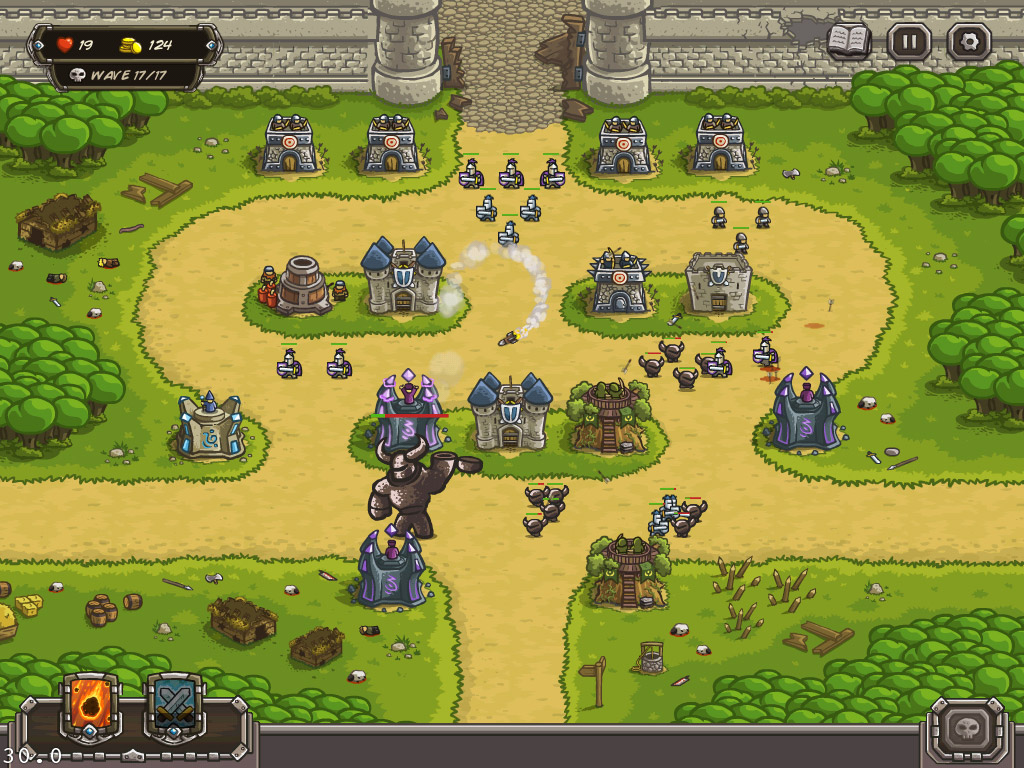
\includegraphics[width=.8\textwidth]{kingdom_rush}
  \caption{Kingdom Rush. Obtida de https://www.ironhidegames.com/Games/kingdom-rush\label{fig:kingdom-rush}}
\end{figure}

\pagebreak

%% ------------------------------------------------------------------------- %%
\section{Shooter}
\label{sec:jogo-ss}

Um \textit{shooter game} é um subgênero de jogos de ação, inspirado pelos jogos de fliperama, por exemplo o jogo  \textit{Spacewar} \citep{Spacewar}, e se estabeleceu com o jogo \textit{Space Invaders} \citep{Space_Invaders}, presente na Figura \ref{fig:space-invaders}. Ambos os jogos funcionam de maneira semelhante, onde uma onda de inimigos deve ser impedida de eliminar o jogador, este podendo se esquivar e atirar neles, sendo que os oponentes também podem dispor de tiros e movimento para causar dano.

%% https://www.gamekult.com/jeux/space-invaders-17318/test.html
\begin{figure}
  \centering
  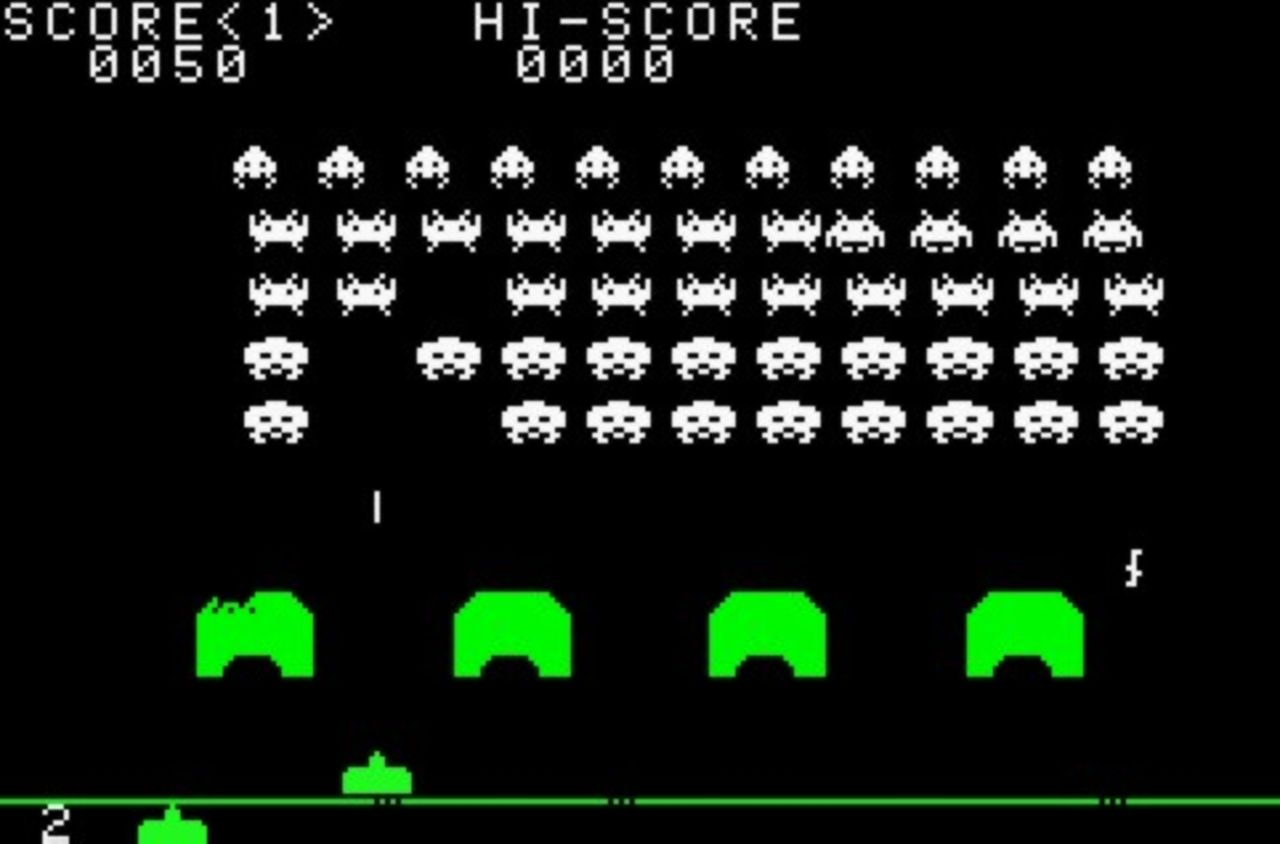
\includegraphics[width=.6\textwidth]{space_invaders}
  \caption{Space Invaders. Obtida de https://www.gamekult.com/jeux/space-invaders-17318/test.html\label{fig:space-invaders}}
\end{figure}

Dentre os elementos comuns ao gênero, existem variações sobre a capacidade do jogador e dos inimigos se moverem no espaço 2D, onde no \textit{Space Invaders} \citep{Space_Invaders}, o jogador possui somente movimento horizontal, enquanto no \textit{Asteroids} \citep{Asteroids}, presente na Figura \ref{fig:asteroids}, o usuário possui movimentação livre em toda área disponível, mas os oponentes não disparam.

%% https://openclipart.org/detail/281726/asteroids-video-games-1979
\begin{figure}
  \centering
  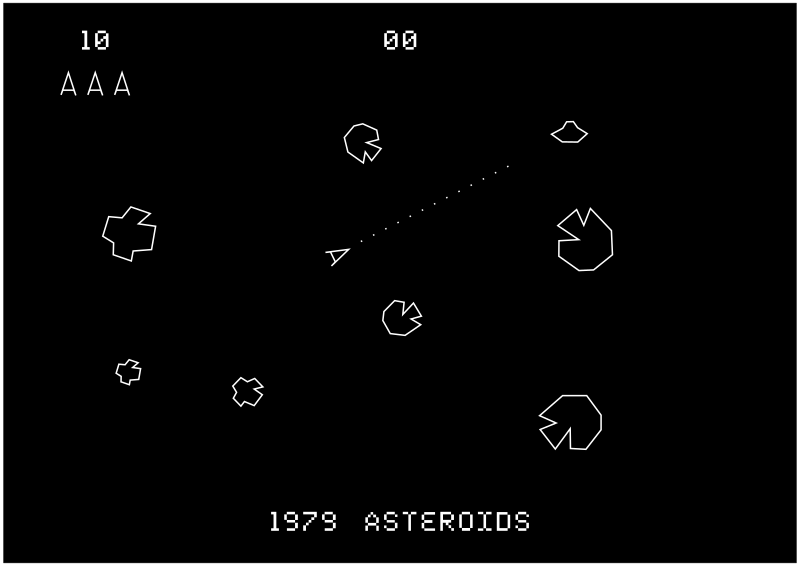
\includegraphics[width=.6\textwidth]{asteroids}
  \caption{Asteroids. Obtida de https://openclipart.org/detail/281726/asteroids-video-games-1979\label{fig:asteroids}}
\end{figure}

%% ------------------------------------------------------------------------- %%
\section{Decisões de Projeto}
\label{sec:jogos-decisoes}

Considerando que são jogos populares e com jogabilidade simples, decidiu-se desenvolver os dois estilos, considerando a simplicidade de seus objetivos em comum, centrados na sobrevivência por meio da habilidade do jogador de se proteger dos inimigos que atacam em turnos, e a possibilidade dos mesmos serem eliminados à distância.

Ao mesmo tempo, enquanto o \textit{Tower Defense} se apresenta de maneira estática - as torres não se movem, e o jogador não pode alterá-las durante a onda - o \textit{Space Shooter} permite movimentação da nave, logo a habilidade motora e reflexos de quem está jogando são fatores na sobrevivência, e seria interessante verificar como essa característica afeta a evolução do algoritmo genético.

Para desenvolver o projeto decidiu-se utilizar ferramentas \textit{Open Source} sempre que possível, a \textit{Godot Game Engine}, versão 3.3.3; a plataforma de versionamento \textit{GitHub}; a comunicação do grupo se concentrou no serviço \textit{Discord}; a monografia foi desenvolvida de maneira colaborativa na plataforma \textit{OverLeaf}; o \textit{Jupyter Notebook} foi utilizado para análise de dados; e o editor de imagens \textit{GIMP} para edição de imagens.
\par

%!TeX root=../tese.tex
%("dica" para o editor de texto: este arquivo é parte de um documento maior)
% para saber mais: https://tex.stackexchange.com/q/78101/183146



%% Nota de rodapé 1: mover para o texto e usar notas de rodapé para citar URLs dos sites de cada engine, com data do último acesso : 

% [p. 7 / § 1] frase de quatro linhas - quebrar em frases mais curtas ou, no caso, montar uma lista de itens. Juntar parágrafo com o seguinte. : X

% [p. 7 / § 2] evitar tantos termos em inglês, principalmente quando eles possuem equivalentes comuns em português:
% open source → código aberto
% license → licença
% game engine → motor de jogos (já que vocês mesmos usaram esse termo no parágrafo anterior)

% Figuras 3.1 e 3.2: citar fonte da imagem : X

% [p. 7 / § 3] escolher ou inglês ou português para se referir aos elementos da Godot e usar de forma consistente (o que ficar em parênteses deve ser só para esclarecer e não o padrão que vocês vão usar). Ajustar no resto da monografia se necessário

% [p. 7 / § 3] sugestão de citação: página de documentação da godot

% [p. 8 / § 2] “todo nó” → “todo nó de colisão/física” ; X
% [p. 8 / § 3] juntar com o parágrafo anterior: X
% [p. 8 / § 3] “programação uma reação” → “programação de uma reação”:X
% [p. 9 / § 4] “figura” -> “Figura” : X

% Figura 3.3: é de vocês? Se for, é legal explicar que ela é do jogo que vocês fizeram. Se não for, citar fonte. : X

% Figura 3.4: se for um exemplo do jogo de vocês, é legal dizer isso. Faltou um ponto final na legenda. : X

% [p. 9 / § 4] typos
% “como um objeto filhos” -> “como objetos filhos” : X

% “a fase geram”: X
% [p. 10 / § 1] juntar com parágrafo anterior : X

%% ------------------------------------------------------------------------- %%
\chapter{Plataforma de Desenvolvimento}
\label{cap:godot}

Para auxiliar na produção de jogos existem diversos motores de jogo ou \textit{Game Engines}; ferramentas que dispõem de recursos e bibliotecas para auxiliar no desenvolvimento. Essas ferramentas oferecem estruturas e métodos para simulação de interações físicas, lidar com a entrada dada pelo usuário, dentre outras funcionalidades. Assim são de grande ajuda para o desenvolvimento do jogo como um todo. A \textit{Godot Engine} é uma  \textit{game engine} de código aberto, usada no desenvolvimento de jogos 2D e 3D, disponibilizada gratuitamente sob \textit{MIT License}. Outros exemplos de \textit{engine} incluem \textit{Unity}\footnote{\url{https://unity.com/pt}}, \textit{Unreal Engine}\footnote{\url{https://www.unrealengine.com/en-US/}} e \textit{RPG Maker}\footnote{\url{https://www.rpgmakerweb.com/}}.


% https://www.unrealengine.com/en-US/
% https://unity.com/pt
% https://www.rpgmakerweb.com/

%% https://godotengine.org/themes/godotengine/assets/press/logo_large_color_light.png
\begin{figure}[htpb]
  \centering
  
\includegraphics[width=.6\textwidth]{godot_logo} 
  \caption{Godot Game Engine.\label{fig:godot-logo} \footnotemark}
\end{figure}
\footnotetext{\url{https://godotengine.org/themes/godotengine/assets/press/logo_large_color_light.png}}

Nesta plataforma, um jogo é um conjunto de cenas composto por nós agrupados em uma estrutura de árvore, estrutura de dado formada por um grafo conexo acíclico. Um nó é a unidade mais básica para construção de elementos, com diferentes propósitos e propriedades, por exemplo, sons, imagens (\textit{sprites}) e câmera. Mesmo com diferentes características e finalidades, todos os nós possuem um nome, variáveis, possibilidade de executarem código (\textit{script}) contendo métodos, herança de funcionalidades ou \textit{script} de outros nós e emissão de sinais de controle para elementos da cena.

\pagebreak

%% https://docs.godotengine.org/en/stable/getting_started/step_by_step/scenes_and_nodes.html
\begin{figure}[htpb]
  \centering
  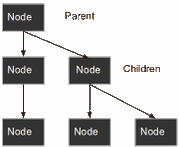
\includegraphics[width=.4\textwidth]{tree}
  \caption{Árvore no Godot.\label{fig:godot-tree} \footnotemark}
\end{figure}
\footnotetext{\url{https://docs.godotengine.org/en/stable/getting_started/step_by_step/scenes_and_nodes.html}}


%% ------------------------------------------------------------------------- %%
\section{Nós}
\label{sec:godot-nos}
 O \textit{Godot} oferece alguns nós específicos para o uso de simulações físicas, fornecendo detecção de colisões entre objetos e diferentes reações caso ocorra o contato. Existem 4 nós específicos para tal função, dependendo do comportamento desejado determinado nó pode ser mais apropriado: \textit{StaticBody2D},  \textit{RigidBody2D}, \textit{KinematicBody2D} e \textit{Area2D}.
 
Todo nó de colisão/física necessita de um filho do tipo \textit{Shape2D} para detectar colisões, pois este fornece a geometria da região que detecta as colisões. Estas podem ocorrer com outros nós ou com as fronteiras da área de jogo. O nó \textit{Area2D} detecta e emite sinais com a presença de outros nós ao seu redor permitindo a programação de uma reação, por exemplo uma esquiva ou animação.

\begin{figure}
  \centering
  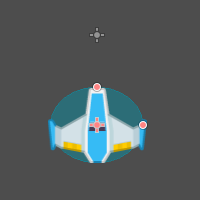
\includegraphics[width=.4\textwidth]{ss/Exemplo area e colisionShape2d.png}
  \caption{Utilizando nós CollisionShape2D e Area2D. Imagem obtida do editor de jogo.\label{fig:area-collision}}
\end{figure}

Na Figura ~\ref{fig:area-collision}, feito para o jogo \textit{Space Shooter}, temos um uso dos nós citados, onde a região em azul sobrepõe a imagem da nave. Esta é um nó do tipo \textit{CollisionShape2D} responsável por detectar colisões com com outros nós, que no jogo são os adversários. A nave por sua vez é um nó do tipo \textit{Area2D} contendo um \textit{sprite} da nave, e quando os nós colidirem, ocorre a emissão de um sinal que terá um comportamento programado, no caso a perda de "vida" do jogador. O conjunto de nós presentes formam uma cena, nesse caso o \textit{Player}.

Nós podem ser agrupados, e o grupo formado atua em conjunto no jogo, conforme a Figura \ref{fig:godot-tree}. O \textit{Tower Defense} e o \textit{SpaceShooter} se aproveitaram de tal característica para a geração dos inimigos e gerenciamento das ondas.

%% ------------------------------------------------------------------------- %%
\section{Sinais}
\label{sec:godot-sinais}

O \textit{Godot} fornece um sistema de sinais, emitidos e detectados por nós, pré-definidos pelo \textit{engine} ou customizados pelo desenvolvedor, que podem servir de gatilhos ou conexões para outras funções em outros nós dentro da hierarquia fornecida pela árvore da cena. As características dos sinais permitem sua utilização em botões na interface, ações em colisões entre nós, entre outras possibilidades.


%% ------------------------------------------------------------------------- %%
\section{Cena}
\label{sec:godot-cena}

A cena no \textit{Godot} é composta de nós organizados segundo uma hierarquia de árvore, onde um nó é a raiz, e seus filhos, que podem ser pais de outros nós, sempre controlados pelo nó raiz, conforme a Figura \ref{fig:scene-tree}, cena feita para o jogo \textit{Space Shooter}. Cenas são objetos independentes, podendo representar somente um elemento do jogo - por exemplo os inimigos, o jogador - ou partes completas dele - como um menu, uma fase.

%% https://docs.godotengine.org/en/stable/getting_started/step_by_step/scenes_and_nodes.html
\begin{figure}
  \centering
  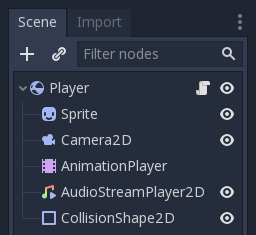
\includegraphics[width=.5\textwidth]{scene_tree_example}
  \caption{Árvore formada por nós no Godot. Em Player um ícone indica a presença de um script vinculado ao nó. Imagem obtida da documentação em \url{https://docs.godotengine.org/en/stable/getting_started/step_by_step/scenes_and_nodes.html}\label{fig:scene-tree}}
\end{figure}



%% ------------------------------------------------------------------------- %%
\section{Instanciação}
\label{sec:godot-instancia}

As cenas de um jogo podem ser inicializadas como objetos filhos de uma outra cena, formando uma instância. Este recurso é usado frequentemente nos jogos desenvolvidos, no \textit{Tower Defense} a fase gera instâncias das cenas das torres e dos inimigos, no \textit{Space Shooter} são instanciados o jogador e os asteróides. As instanciações são feitas de maneira dinâmica durante o jogo, sendo carregadas pelos \textit{scripts} e esperando o \textit{input} do jogador, para a instanciação de um novo objeto que é inserido na árvore de execução. É possível observar o uso da instanciação na Figura \ref{fig:instancia-tiro}, onde a partir do \textit{input} do jogador, projeteis são postos na cena em execução. Cada projetil é uma instanciação, ou objeto, de uma cena feita anteriormente para ser os tiros vistos no jogo.

\begin{figure}
  \centering
  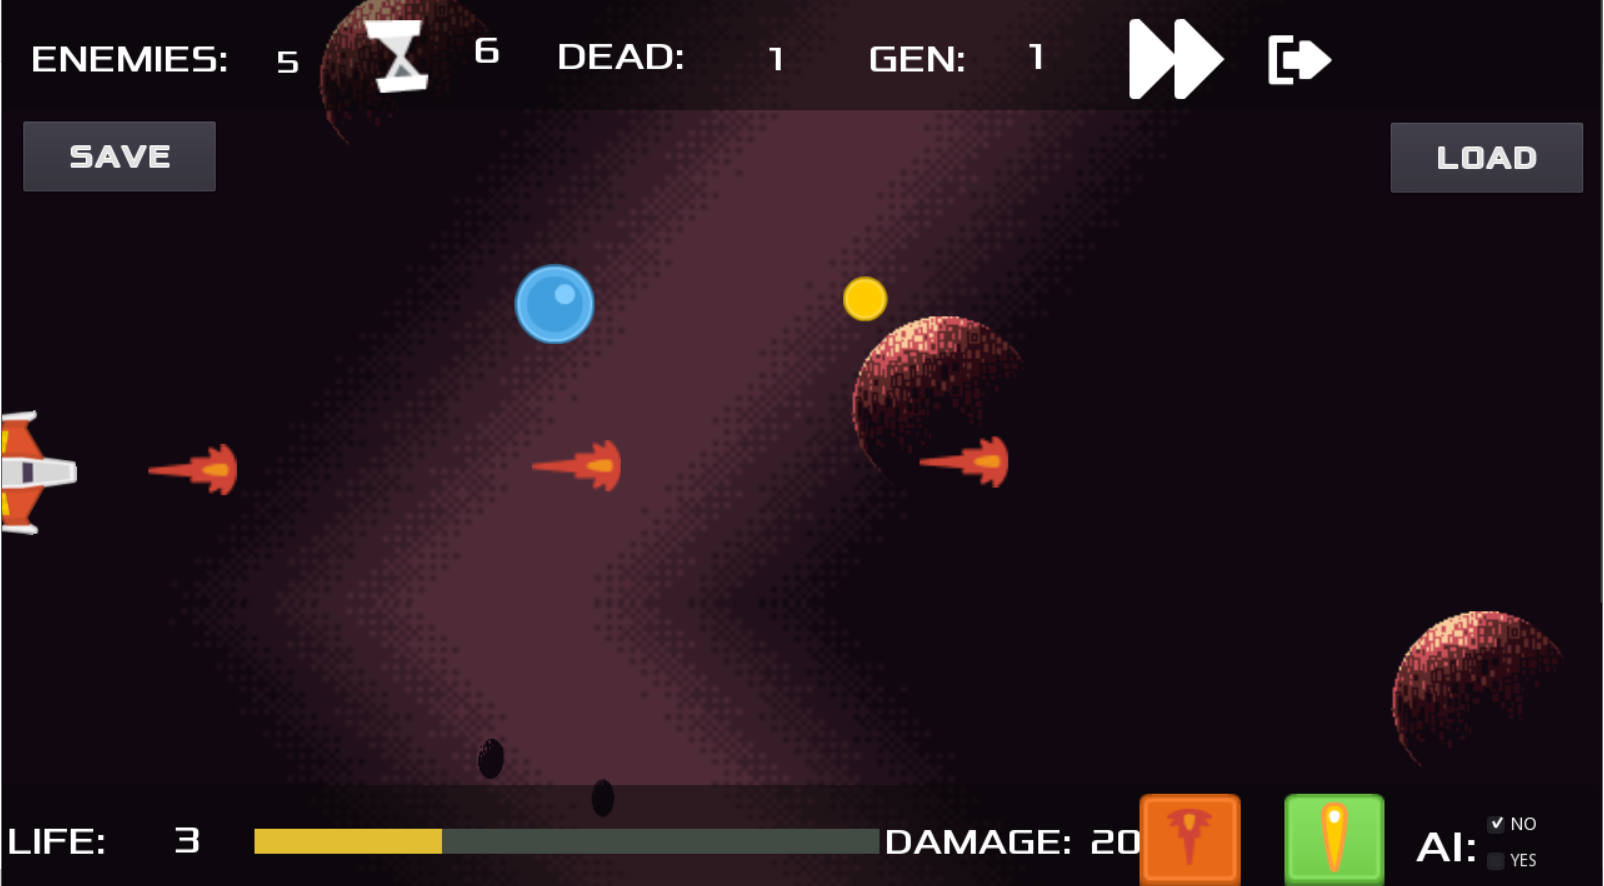
\includegraphics[width=.8\textwidth]{ss/instanciao tiros ss.png}
  \caption{Instanciação de tiros no Space Shooter. Imagem retirada do próprio jogo.\label{fig:instancia-tiro}}
\end{figure}


%% ------------------------------------------------------------------------- %%
\section{Singletons}
\label{sec:godot-singleton}

\textit{Singletons} fornecem a possibilidade de acesso global a métodos e variáveis de outras classes no \textit{Godot}. Semelhante aos sinais, os \textit{singletons} oferecem comunicação entre cenas distintas, relevantes no projeto pois permitiu a implementação do algoritmo genético, que necessita de acesso a diversas variáveis dos jogos, como os inimigos, dano causado, entre outros.

%% ------------------------------------------------------------------------- %%
\section{GDscript}
\label{sec:godot-gdscript}

% Recomendação Will: juntar paragrafos.

Os \textit{scripts} citados são escritos em \textit{GDscript}, linguagem de programação dinâmica de alto nível desenvolvida especificamente para a \textit{Godot Engine}, similar a linguagem de programação \textit{Python} e \textit{Lua}, porém com otimizações e tipos de dados específicos, altamente integrado à própria \textit{engine}\citep{godot-faq}. O editor fornecido integra diversas funcionalidades de um ambiente de desenvolvimento avançado em sua interface, como editor visual 2D e 3D, editor de texto, conexões de sinais, depurador, visualização da árvore de execução durante o desenvolvimento e em tempo real durante a execução, que facilitam o início da produção de jogos.

%% ------------------------------------------------------------------------- %%
\section{Desenvolvimento dos jogos}
\label{sec:desenvolvimento}


% Mencionar o uso de licenças abertas
Para facilitar a familiarização com o ambiente de desenvolvimento e acelerar o foco no algoritmo genético, foram utilizados diversos recursos disponíveis para a produção dos jogos. Desde repositórios de \textit{sprites} como \citet{Kenny_sprites} a tutoriais de \textit{Godot}, sendo o \textit{Space Shooter} baseado no tutorial de \citet{Godot_Linietsy}, disponível na documentação da \textit{engine}, enquanto o \textit{Tower Defense} foi baseado no tutorial disponibilizado pelo \citet{GameDevelopmentCenter21:tdtutorial}. Tanto \citet{Kenny_sprites} como \citet{Godot_Linietsy} possuem licenças que permitem o uso publico ou equivalente, além de serem gratuitas.  

\par

%!TeX root=../tese.tex
%("dica" para o editor de texto: este arquivo é parte de um documento maior)
% para saber mais: https://tex.stackexchange.com/q/78101/183146

%% ------------------------------------------------------------------------- %%

%Recomendação WILL: 
% Ao invés de mecânica colocar design : X
% TD Mencionar Tabelas : X
% TD Mencionar Figuras 4.1 , 4.2, 4.4, 4.5 : X
% SS Mencionar Tabelas : 4.3,  4.4: X
% SS Mencionar Figuras:  4.7, 4.8, 4.9, 4.10, 4.11, 4.12:X

\chapter{Design dos jogos}
\label{cap:mecanica-dos-jogos}

O desenvolvimento dos jogos foi focado em características comuns entre si, para possibilitar o uso do mesmo algoritmo genético, minimizando a necessidade de ajustes no código. A implementação inicial foi feita no \textit{Tower Defense}, e em seguida no \textit{Space Shooter}.

%% ------------------------------------------------------------------------- %%
\section{Tower Defense}
\label{sec:mj-td}

\subsection{O jogo}
\label{sub-sec:jogo-td}

O jogo \textit{Tower Defense} \footnote{Repositório contendo o jogo: { \url{https://github.com/raktanaka/tccTD} - 21/12/2021}} consiste em mapa com dois caminhos a serem percorridos por tanques inimigos e oferece ao jogador duas torres para impedir que os tanques completem seu trajeto. O início do percurso é na esquerda da tela, terminando na direita, conforme visto na Figura \ref{fig:td-inicial}.

\begin{figure}
  \centering
  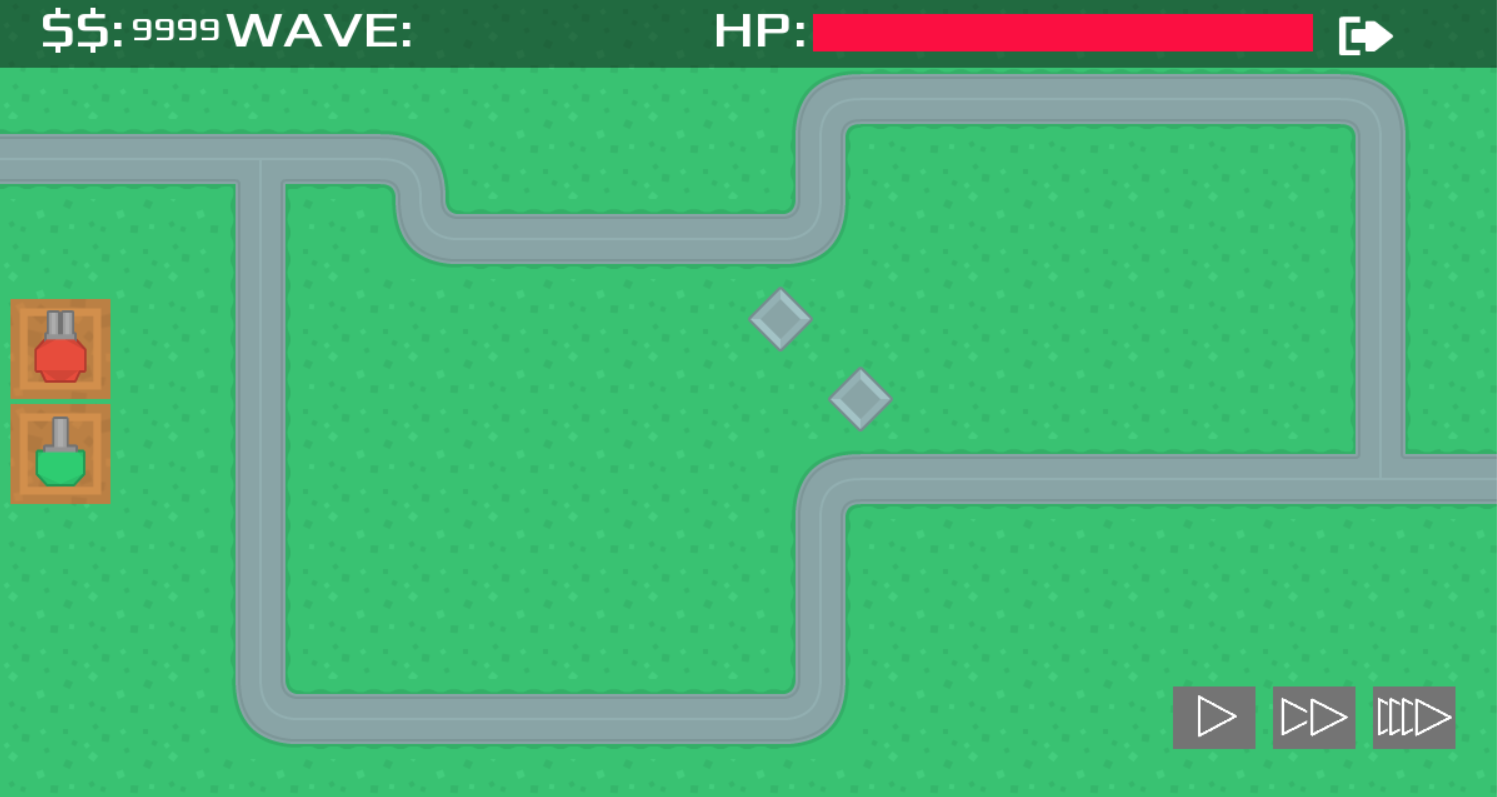
\includegraphics[width=\textwidth]{td/Mapa_inicial_tDD.png}
  \caption{Tela Inicial. Imagem retirada do próprio jogo.\label{fig:td-inicial}}
\end{figure}

Antes de apertar o botão \textit{Play}, o jogador pode colocar quantas e quaisquer torres desejar em áreas livres do mapa. Iniciando a partida, uma onda de 12 tanques começa a percorrer o caminho, inicialmente 6 para cada percurso, conforme a Figura \ref{fig:td-exemplo}. Posteriormente, o algoritmo genético gerencia a rota. Ao lado do botão \textit{Play} estão botões que aceleram a execução do jogo em duas vezes e oito vezes, para facilitar a coleta de dados para os testes.

As duas torres disponíveis oferecem diferentes áreas de alcance para detecção de tanques, apresentadas nas Figuras \ref{fig:td-range-gree} e \ref{fig:td-range-red} e quantidade de dano que podem causar, como esta descrito na Tabela \ref{tab:dados_torres}. Cada inimigo que atinge o objetivo produz dano ao jogador, que possui 100 pontos de vida, mostrado pela barra \textit{HP} na tela. A região também mostra os recursos monetários disponíveis ao jogador - que não está implementado - e a onda atual; o jogo somente termina quando acaba o \textit{HP} do jogador.

\begin{figure}
  \centering
  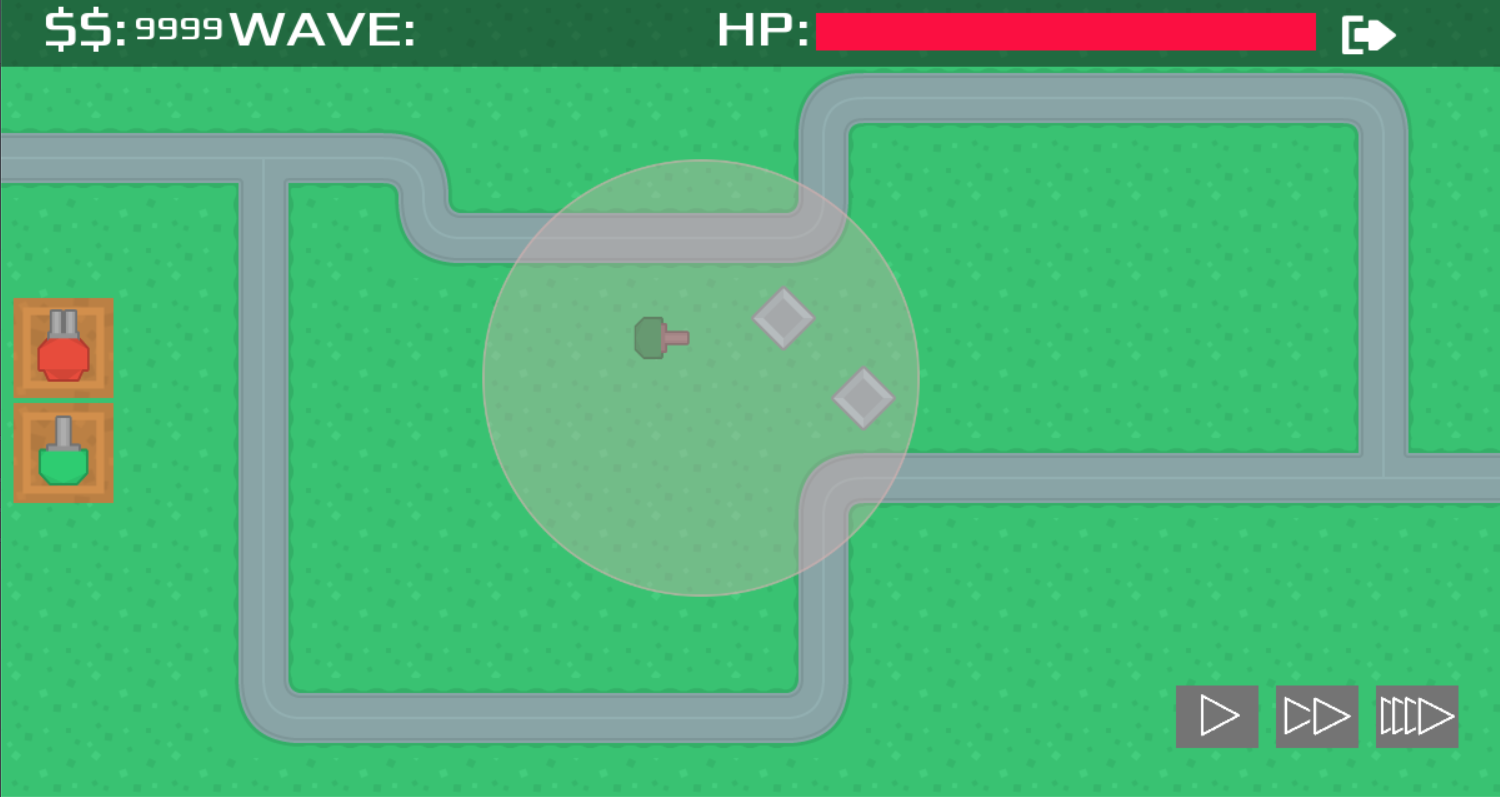
\includegraphics[width=0.8\textwidth]{td/range_green_tower.png}
  \caption{Área de detecção torre verde. Imagem retirada do próprio jogo.\label{fig:td-range-gree}}
\end{figure}

\begin{figure}
  \centering
  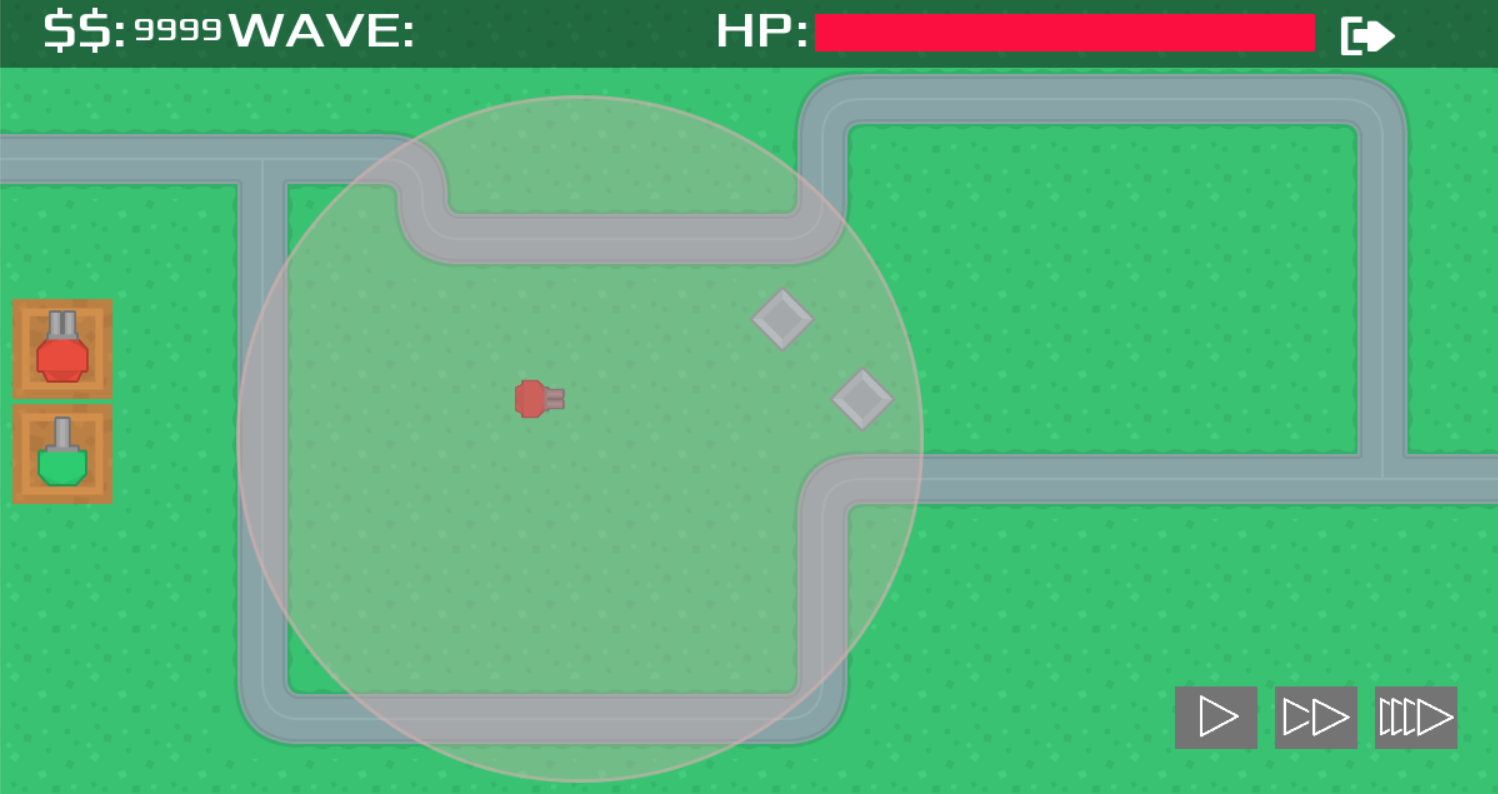
\includegraphics[width=0.8\textwidth]{td/range_red_tower.png}
  \caption{Área de detecção torre vermelha. Imagem retirada do próprio jogo.\label{fig:td-range-red}}
\end{figure}

\begin{table}[H]
\caption{Dano das torres no Tower Defense.\label{tab:dados_torres}}
\begin{tabular}{c|ccc}

               & velocidade de tiro  & dano   & alcance\\ \hline
Torre Verde    & 55                  & 25     &  350 \\
Torre Vermelha & 70                  & 15     &  550       

\end{tabular}
\end{table}


\begin{figure}
  \centering
  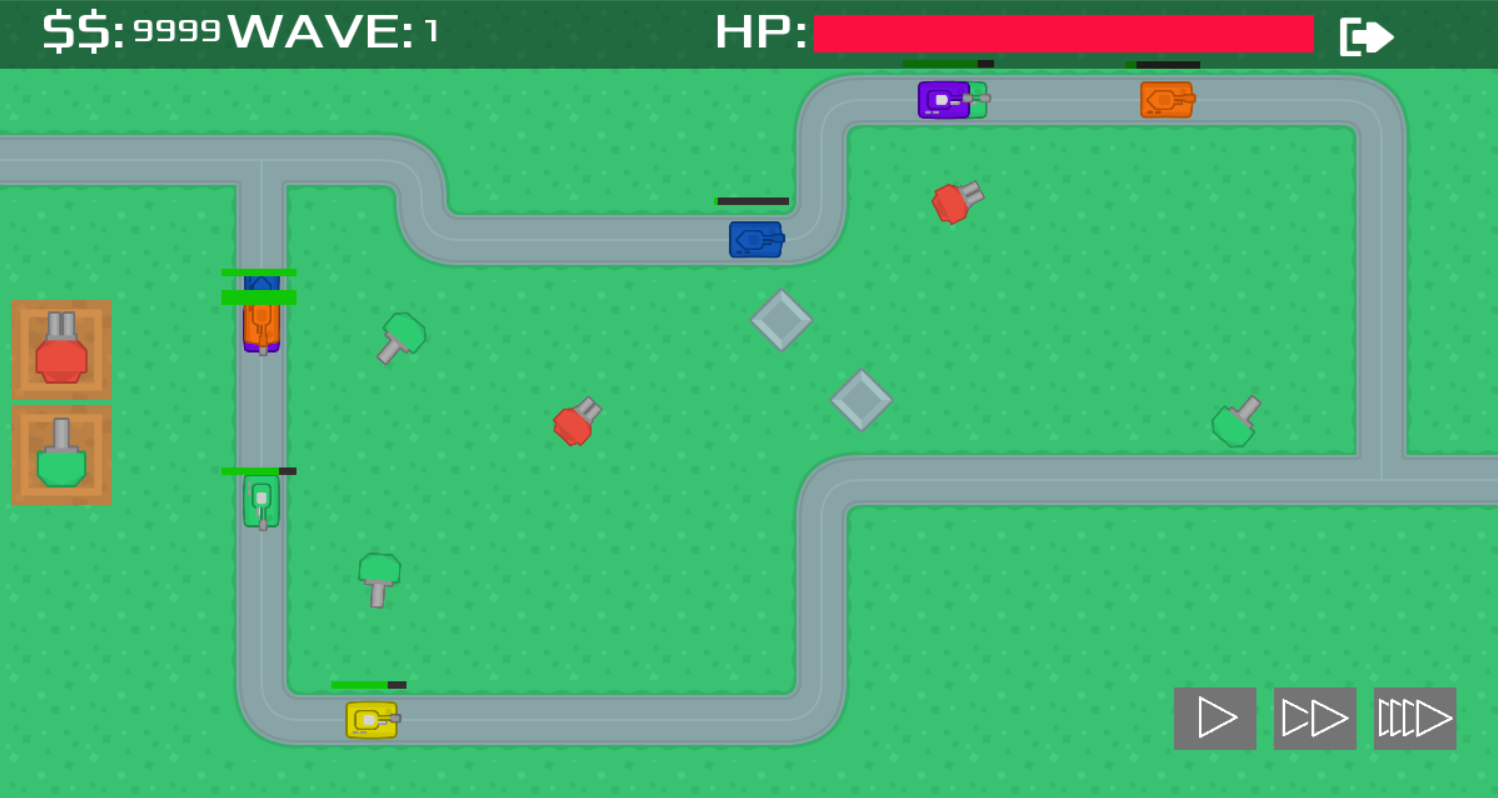
\includegraphics[width=\textwidth]{td/exemplo de execução TDD.png}
  \caption{Exemplo de uma execução do jogo. Imagem retirada do próprio jogo.\label{fig:td-exemplo}}
\end{figure}


Existem 6 tipos de tanques diferentes, descritos na Figura \ref{fig:figure-tipos-tanque}. Cada tipo de tanque possui 2 características, sendo elas velocidade e dano causado ao jogador, cujo os valores variam conforme o tipo, visto a Tabela \ref{tab:tank-dmg}. 

\begin{figure}
     \centering
     \begin{subfigure}[b]{0.2\textwidth}
         \centering
         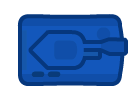
\includegraphics[width=\textwidth]{td/tank_blue.png}
         \caption{tank blue}
         \label{fig:td-tank-blue}
     \end{subfigure}
     \hfill
     \begin{subfigure}[b]{0.2\textwidth}
         \centering
         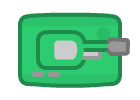
\includegraphics[width=\textwidth]{td/tank_green.png}
         \caption{tank green}
         \label{fig:td-tank-green}
     \end{subfigure}
     \hfill
     \begin{subfigure}[b]{0.2\textwidth}
         \centering
         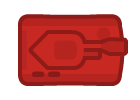
\includegraphics[width=\textwidth]{td/tank_red.png}
         \caption{tank red}
         \label{fig:td-tank-red}
     \end{subfigure}
     
     \begin{subfigure}[b]{0.2\textwidth}
         \centering
         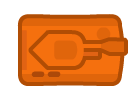
\includegraphics[width=\textwidth]{td/tank_orange.png}
         \caption{tank orange}
         \label{fig:td-tank-orange}
     \end{subfigure}
     \hfill
     \begin{subfigure}[b]{0.2\textwidth}
         \centering
         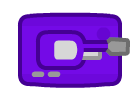
\includegraphics[width=\textwidth]{td/tank_purple.png}
         \caption{tank purple}
         \label{fig:td-tank-purple}
     \end{subfigure}
     \hfill
     \begin{subfigure}[b]{0.2\textwidth}
         \centering
         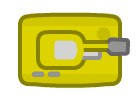
\includegraphics[width=\textwidth]{td/tank_yellow.png}
         \caption{tank yellow}
         \label{fig:td-tank-yellow}
     \end{subfigure}     
     \caption{Tipos de tanques}
     \label{fig:figure-tipos-tanque}
\end{figure}

\newpage

\begin{table}
\caption{Dano de cada tanque no Tower Defense}
\begin{tabular}{c|cc}
            & velocidade & dano   \\ \hline
tank blue   & 55    & 55         \\
tank green  & 70    & 45         \\
tank red    & 80    & 15          \\
tank orange & 120   & 5           \\
tank purple & 90    & 15          \\
tank yellow & 150   & 5           
\end{tabular}
\label{tab:tank-dmg}
\end{table}

Ficam definidas como Norte e Sul as rotas disponíveis, na Figura \ref{fig:td-rota}.

\begin{figure}
  \centering
  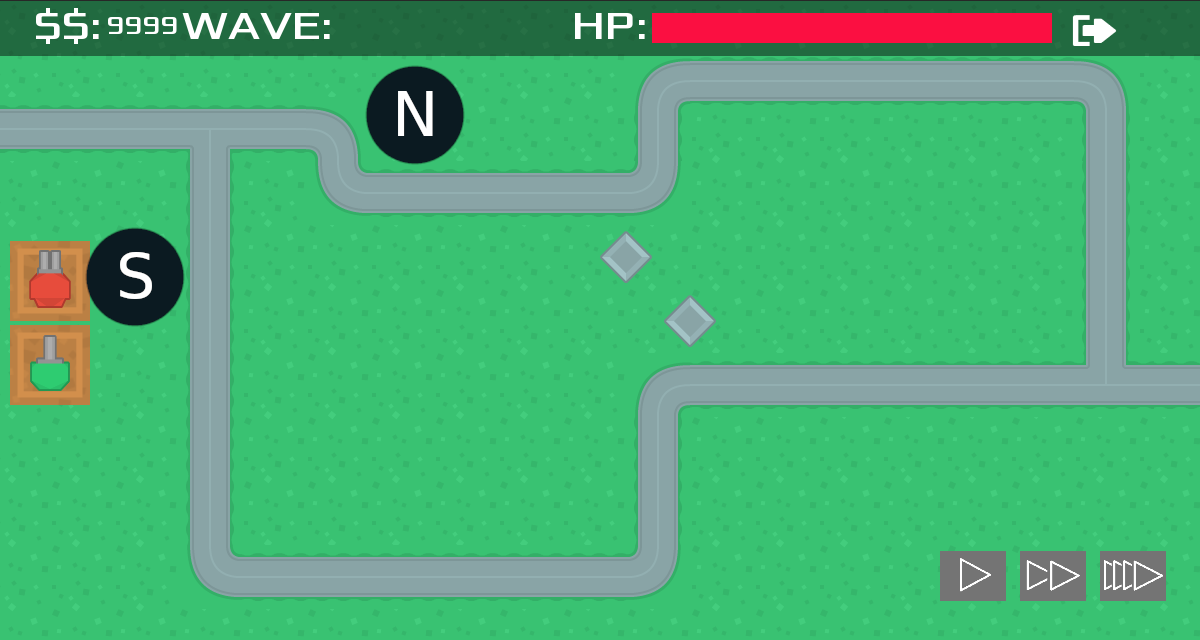
\includegraphics[width=\textwidth]{td/td_positions.png}
  \caption{Definição das rotas Norte e Sul. Imagem retirada do jogo e editada.\label{fig:td-rota}}
\end{figure}

\subsection{Mecânica de Resistência}
\label{sub-sec:mecanica-de-resistencia}

No jogo de \textit{Tower Defense} também foi adicionado um sistema de resistência nos tanques, cada Tanque possui resistência contra Torres de \textbf{mesma cor} e recebem dano reduzido pela metade dos mesmos. Segue um pseudocódigo da implementação do tanque ao receber dano de uma torre.

\begin{programruledcaption}{Sistema de Resistência TD.\label{prog:resistencia-TD}}
  \begin{lstlisting}[
    language={[brazilian]pseudocode},
    style=pseudocode,
    style=wider,
    functions={},
    specialidentifiers={},
  ]
        // x = tanque que recebe o dano
        // damage = quantidade total de dano recebido
        // color\_tower = cor da torre que disparou no tanque.
        func on_hit(x, damage, color_tower):
            // color (x) = cor do tanque \textbf{x}
            //  hp(x) = hp atual de x.
	        se color (x) = color_tower:
		        hp (x) -= damage / 2
		
        	senao:
        		hp (x) -= damage
        fim
  \end{lstlisting}
\end{programruledcaption}


\newpage
%% ------------------------------------------------------------------------- %%
\section{Space Shooter}
\label{sec:mj-ss}

O jogo \textit{Space Shooter}\footnote{Repositório contendo o jogo { \url{https://github.com/RGPRafael/godot} - 21/12/2021}} consiste em uma nave que o jogador pode mover livremente em um espaço 2D, onde este deve sobreviver a ondas de asteroides que partem de diferentes posições da tela em sua direção. O jogador além de esquivar, pode eliminar os asteroides por meio de disparos com o \textit{mouse}. 

\begin{figure}
  \centering
  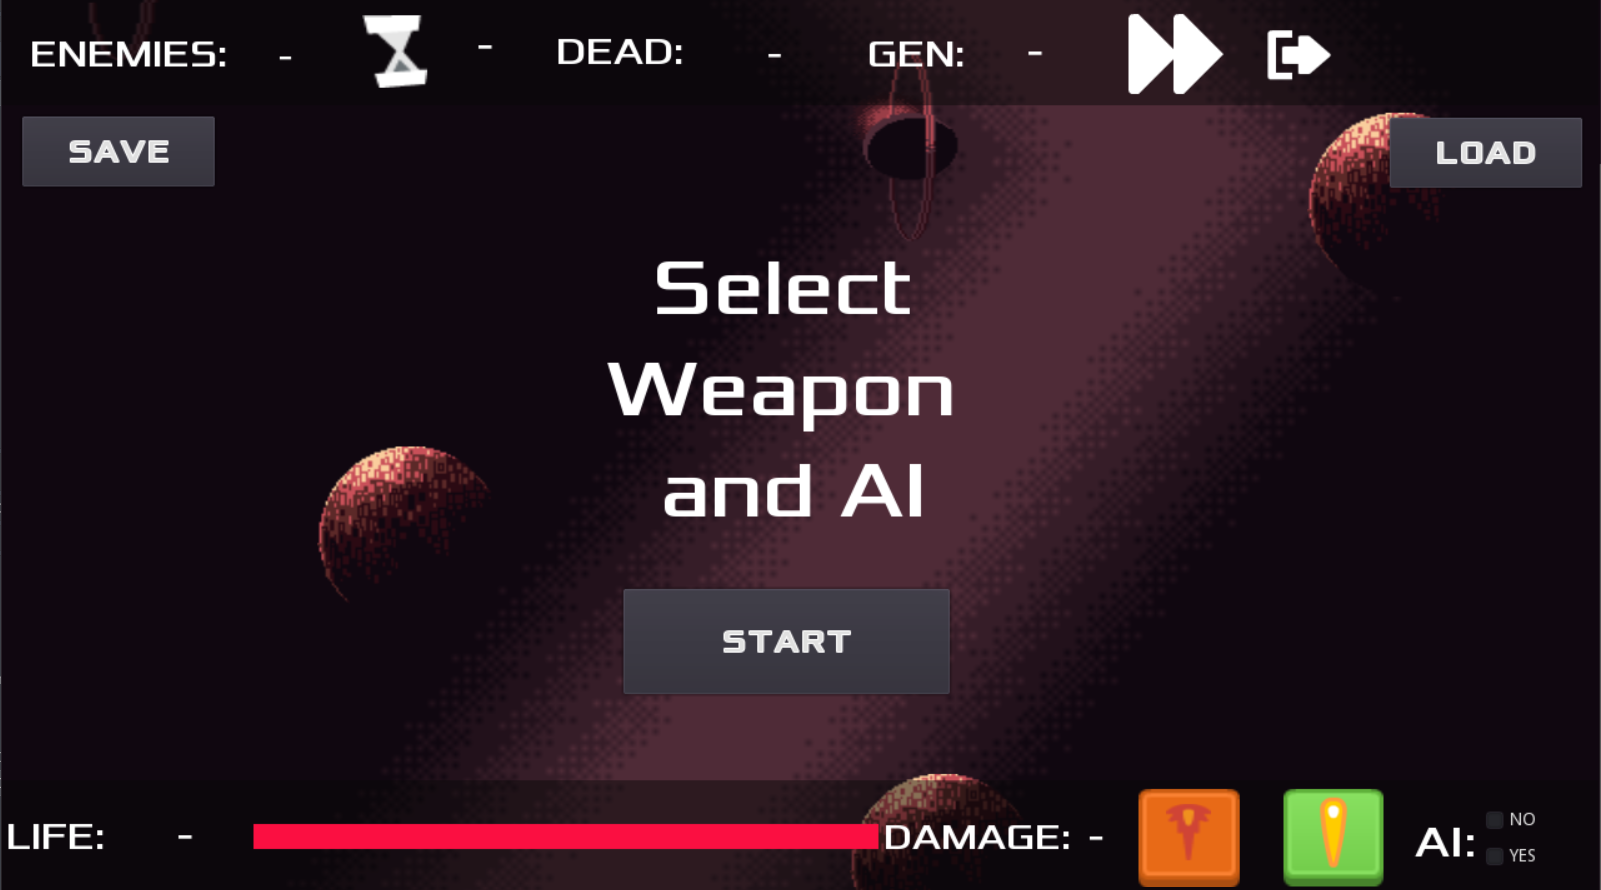
\includegraphics[width=\textwidth]{ss/Tela_inicial_space_shooter.png}
  \caption{Tela inicial. Imagem retirada do próprio jogo.\label{fig:ss-start}}
\end{figure}

Existem dois tipos de disparos que o jogador pode usar para sua defesa, cada um com características diferentes. No começo do jogo é requisitado que o jogador escolha qual tipo de disparo irá utilizar, conforme as Figuras \ref{fig:ss-start} e \ref{fig:ss-disparos}.

\begin{figure}
     \centering
     \begin{subfigure}[b]{0.15\textwidth}
         \centering
         
\includegraphics[width=\textwidth]{ss/Disparo_.png}
         \caption{Disparo}
         \label{fig:ss-disparo}
     \end{subfigure}
     \begin{subfigure}[b]{0.15\textwidth}
         \centering
         
\includegraphics[width=\textwidth]{ss/Disparo1_.png}
         \caption{Disparo1}
         \label{fig:ss-disparo1}
     \end{subfigure}
     \caption{Disparos}
     \label{fig:ss-disparos}
\end{figure}

\begin{table}
\caption{Dano dos tiros no Space Shooter}
\begin{tabular}{c|cc}
          & Velocidade de Tiro & Dano \\ \hline
Disparo   & 1200  & 15     \\
Disparo 1 & 600   & 30    
\end{tabular}
\label{tab:tiro=-ss}
\end{table}

Existem dois tipos de \textit{player} automáticos disponíveis para escolha, caso o jogador marque a opção \textit{'yes'} na barra inferior, próximo ao texto \textit{'AI'}, como pode se observar na Figura \ref{fig:ss-player-ai}. Tais \textit{players} foram desenvolvidos com o intuito de auxiliar no projeto, e na realização dos testes e coleta de dados. Uma delas faz com que a nave transite da direita para esquerda em um intervalo de cinco minutos, a outra opção faz com que a nave fique parada no meio da tela, em ambos atirando no inimigo mais próximo que detectar, de forma a destruir o asteroide que vem em sua direção ou ser atingida.  

\begin{figure}
  \centering
  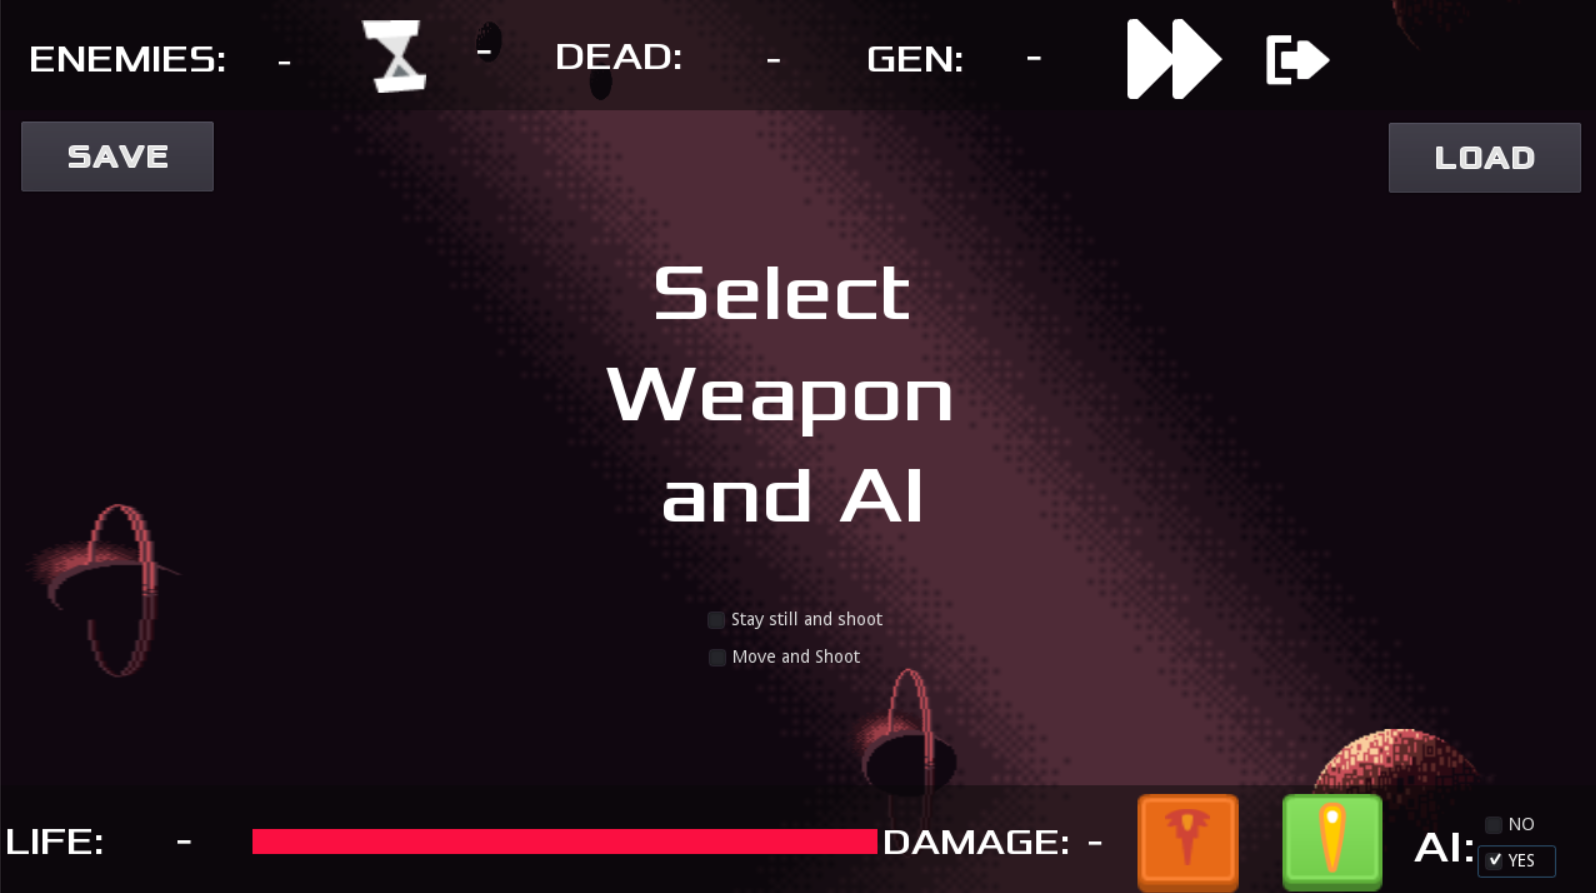
\includegraphics[width=\textwidth]{ss/Escolhendo player automatico.png}
  \caption{Opções de Player Automático. Imagem retirada do próprio jogo.\label{fig:ss-player-ai}}
\end{figure}


Existem 6 tipos de asteroides diferentes, presentes na Figura \ref{fig:ss-tipo-ast}. Cada tipo de asteroide possui 3 características, sendo elas velocidade, vida ou resistência e dano causado ao jogador, cujo os valores variam conforme o tipo, presentes na Tabela \ref{tab:ss-ast-dmg}. 

\begin{figure}
     \centering
     \begin{subfigure}[b]{0.15\textwidth}
         \centering
         
\includegraphics[width=\textwidth]{ss/inimigos.png}
         \caption{inimigos}
         \label{fig:ss-inimigos}
     \end{subfigure}
     \hfill
     \begin{subfigure}[b]{0.15\textwidth}
         \centering
         
\includegraphics[width=\textwidth]{ss/inimigo1.png}
         \caption{inimigo1}
         \label{fig:ss-inimigo1}
     \end{subfigure}
     \hfill
     \begin{subfigure}[b]{0.15\textwidth}
         \centering
         
\includegraphics[width=\textwidth]{ss/inimigo2.png}
         \caption{inimigo2}
         \label{fig:ss-inimigo2}
     \end{subfigure}

     \begin{subfigure}[b]{0.15\textwidth}
         \centering
         
\includegraphics[width=\textwidth]{ss/inimigo3.png}
         \caption{inimigo3}
         \label{fig:ss-inimigo3}
     \end{subfigure}
     \hfill
     \begin{subfigure}[b]{0.15\textwidth}
         \centering
         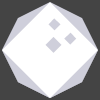
\includegraphics[width=\textwidth]{ss/inimigo4.png}
         \caption{inimigo4}
         \label{fig:ss-inimigo4}
     \end{subfigure}
     \hfill
     \begin{subfigure}[b]{0.15\textwidth}
         \centering
         
\includegraphics[width=\textwidth]{ss/inimigo5.png}
         \caption{inimigo5}
         \label{fig:figure-inimigos}
     \end{subfigure}     
     \caption{Tipos de asteroides}
     \label{fig:ss-tipo-ast}
\end{figure}

\begin{table}[H]
\caption{Velocidade, dano e vida de cada asteroide no Space Shooter}
\begin{tabular}{c|ccc}
         & Velocidade & Dano & Vida   \\ \hline
inimigos & 500        & 20     &   50     \\
inimigo1 & 350        & 45     &   30     \\
inimigo2 & 470        & 50     &   40     \\
inimigo3 & 320        & 60     &   40     \\
inimigo4 & 550        & 20     &   60     \\
inimigo5 & 700        & 10     &   120      
\end{tabular}
\label{tab:ss-ast-dmg}
\end{table}

Após feitas as escolhas sobre o tipo de disparo que será utilizado e se o jogador vai mover a nave ou não, basta apertar o botão \textit{'Start'} para inicio do jogo. O jogador assim deve sobreviver às ondas de inimigos que aparecem de diferentes posições da tela. 

Caso seja atingido, a quantidade de dano que sofreu é exibida no campo \textit{'Damage'}. Por sua vez, quantidade de inimigos que apareceram enquanto o jogo ainda se desenrola é mostrada na barra superior na extrema esquerda, assim como outras informações como numero de asteroides que foram mortos e o números de gerações que foram enfrentadas. Há um botão para acelerar a velocidade do jogo, e outro que volta ao começo do jogo, caso o jogador não queria continuar ou tenha se arrependido das configurações iniciais que fez anteriormente, um exemplo de uma rodada do jogo encontra-se na Figura \ref{fig:ss-exemplo}.

\begin{figure}
  \centering
  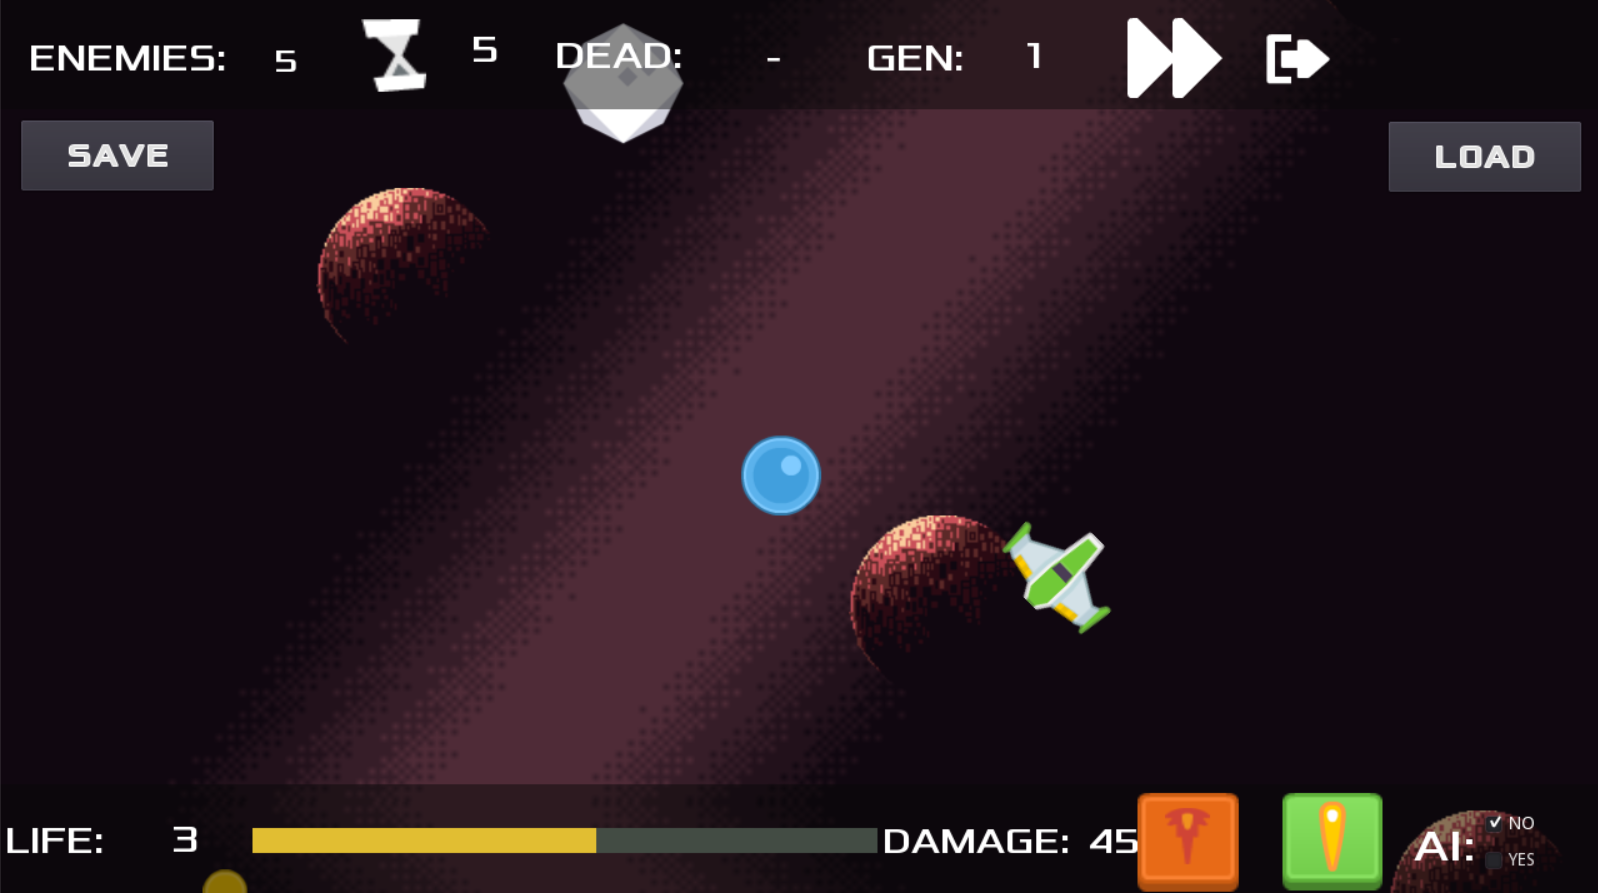
\includegraphics[width=\textwidth]{ss/Exemplo de jogo.png}
  \caption{Exemplo de uma rodada do jogo. Imagem retirada do próprio jogo.\label{fig:ss-exemplo}}
\end{figure}

O jogador começa com a sua barra de vida no valor total igual a 100. Caso chegue a zero 3 vezes o jogador morre e o jogo volta à tela inicial onde as configurações sobre a escolha de arma, por exemplo, devem ser feitas de novo. Ficam definidos os locais de \textit{spawn} de 1 até 6 na Figura \ref{fig:ss-positions}

\begin{figure}
  \centering
  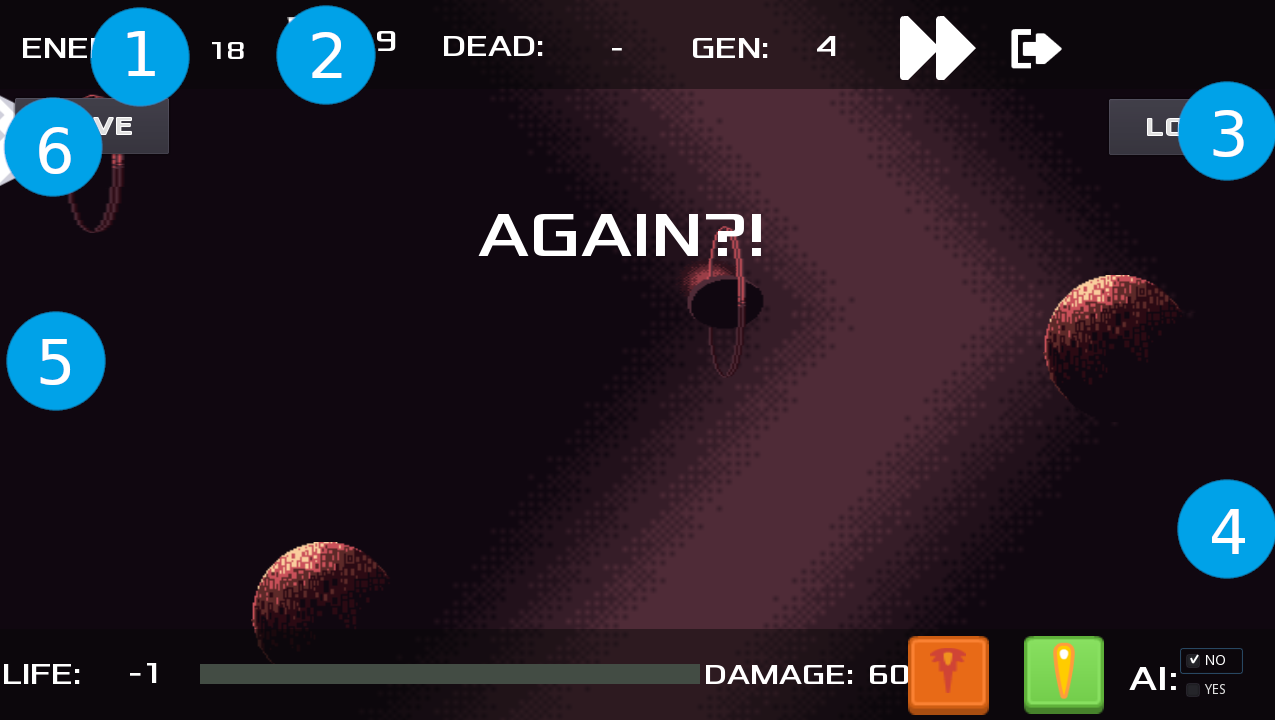
\includegraphics[width=\textwidth]{ss/ss_positions.png}
  \caption{Posições possíveis onde um asteroide pode surgir. Imagem retirada do jogo e editada.\label{fig:ss-positions}}
\end{figure}
\par

%!TeX root=../tese.tex
%("dica" para o editor de texto: este arquivo é parte de um documento maior)
% para saber mais: https://tex.stackexchange.com/q/78101/183146

%% ------------------------------------------------------------------------- %%
\chapter{Algoritmo Genético}
\label{cap:algoritmo-genetico}

Algoritmo genético é uma técnica de evolução computacional desenvolvida para o estudo de comportamento adaptativo \citep{eiben15:introga}. De maneira simplificada, o algoritmo cria um conjunto de diferentes resoluções para um dado problema e, a partir da avaliação desse conjunto, seleciona as melhores soluções.

Esse processo imita a ideia de seleção natural proposta por Darwin \citep{eiben15:introga}, onde os indivíduos de uma população disputam por recursos para sobreviverem. Aqueles que sobrevivem conseguem passar seus genes para a prole e a população seguinte será mais adaptada ao ambiente e com mais chances de reprodução, passando as características que permitiram sua sobrevivência para as gerações seguintes. Portanto, um algoritmo genético é composto das seguintes etapas: Inicialização, Avaliação, Seleção, Cruzamento \textit{(Cross over)}, Mutação e Atualização (Figura ~\ref{fig:alg-genetico} ).

%% ------------------------------------------------------------------------- %%
\section{O Algoritmo}
\label{sec:ag-algoritmo}

No projeto, cada indivíduo é um inimigo criado pelo jogo e a população se resume a uma \textit{"wave"} (onda de inimigos). Os genes representam características importantes dos inimigos, como: Tipo (TD e SS), Rota (TD), Local de \textit{Spawn} (SS), conforme esboçado por \citet{mallawaarachchi:gatutorial} e \citet{ahmed18:tutorialgapython}.

%% FALTA REFERÊNCIA DA IMAGEM
\begin{figure}
  \centering
  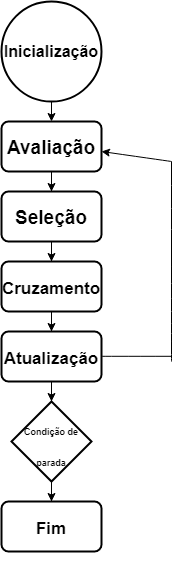
\includegraphics[width=4cm]{alg_genetico2}
  \caption{Estrutura de um algoritmo genético.\label{fig:alg-genetico}}
\end{figure}


%% ------------------------------------------------------------------------- %%
\subsection{Inicialização}
\label{sec:ag-inicializacao}

Na primeira etapa, inicialização, são codificados os genes para que sejam submetidos ao processo de avaliação. 

\pagebreak

\begin{programruledcaption}{Inicialização do \textit{Space Shooter} com tipo de inimigo e local de surgimento.\label{prog:init-ss}}
  \begin{lstlisting}[
    language={[brazilian]pseudocode},
    style=pseudocode,
    style=wider,
    functions={},
    specialidentifiers={},
  ]
var population = [['inimigos',Vector2(90,-50) ], 
                 ['inimigo1',Vector2(90,-50)], 
                 ['inimigo2',Vector2(90,-50)], 
                 ['inimigo3',Vector2(90,-50)], 
                 ['inimigo4',Vector2(90,-50) ],
                 ['inimigo5',Vector2(90,-50)]]
  \end{lstlisting}
\end{programruledcaption}

\begin{programruledcaption}{Inicialização do \textit{Tower Defense} com tipo de inimigo e rota.\label{prog:init-td}}
  \begin{lstlisting}[
    language={[brazilian]pseudocode},
    style=pseudocode,
    style=wider,
    functions={},
    specialidentifiers={},
  ]
var population = [['EnemyRed', 0], ['EnemyGreen', 0], ['EnemyBlue', 0],
                 ['EnemyYellow', 0], ['EnemyPurple', 0], ['EnemyOrange', 0],
                 ['EnemyRed', 1], ['EnemyGreen', 1], ['EnemyBlue', 1],
                 ['EnemyYellow', 1], ['EnemyPurple', 1], ['EnemyOrange', 1]]
  \end{lstlisting}
\end{programruledcaption}

No \textit{Tower Defense} o algoritmo inicia com uma população de 12 inimigos, 1 de cada tipo para cada rota; no \textit{Space Shootes} são 1 de cada tipo em cada posição de \textit{spawn}. Uma amostra que pareceu adequada para o propósito do experimento, uma vez que populações pequenas convergem mais rapidamente, economizando tempo para múltiplas execuções,e não tem indícios de serem piores do que largas populações. \citet{haupt00:mutationprob}

%% ------------------------------------------------------------------------- %%
\subsection{Avaliação}
\label{sec:ag-avaliacao}

A avaliação (ou função \textit{Fitness}) realiza uma análise que estabelece o quão bem os indivíduos da população resolvem o problema proposto. Na natureza, se trata da habilidade de um indivíduo competir contra os demais da população, no algoritmo proposto segue:

\begin{programruledcaption}{\textit{Fitness} do \textit{Tower Defense} (Avaliação, em português).\label{prog:avaliacao_TD}}
  \begin{lstlisting}[
    language={[brazilian]pseudocode},
    style=pseudocode,
    style=wider,
    functions={},
    specialidentifiers={},
  ]
        funcao fitness_TD (x) // Dá uma pontuação para indivíduo \textbf{x}
            // offset (x) = quanto do caminho foi percorrido, float de 0 a 1.
            // hp (x)     = quanto de HP sobrou do inimigo, float de 0 a 1.
	        fit := (offset (x) + hp (x)) / 2 // média aritmética dos valores de x
	        devolva fit // Um float com uma pontuação no intervalo [0,1].
        fim
  \end{lstlisting}
\end{programruledcaption}

\begin{programruledcaption}{\textit{Fitness} do \textit{Space Shooter} (Avaliação, em português).\label{prog:avaliacao_SS}}
  \begin{lstlisting}[
    language={[brazilian]pseudocode},
    style=pseudocode,
    style=wider,
    functions={},
    specialidentifiers={},
  ]
        funcao fitness_SS (x) // Dá uma pontuação para indivíduo \textbf{x}
            // reached-goal (x) = booleana se acertou o inimigo ou nao
            se reached-goal
                fit := 5
            senao
                fit := 0
            
            // hp(x) = 5 * quanto de HP sobrou do inimigo (mob), no intervalo [0,1]
	        fit := (fit + hp(x)) / 10 // média aritmética dos valores de x
	        devolva fit // Um float com uma pontuação no intervalo [0,1].
        fim
  \end{lstlisting}
\end{programruledcaption}

Deve ser ressaltado que o \textit{fitness} é uma característica inerente a cada sistema, com múltiplas possibilidades de avaliação que produzem resultados que podem ser considerados corretos, encontrando máximos locais que satisfazem os problemas propostos.

%%
%% FALTA REFERÊNCIA DA IMAGEM
%%\begin{figure}
%%  \centering
%%  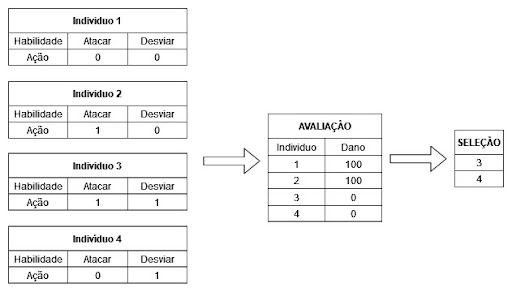
\includegraphics[width=.8\textwidth]{tabel_gen_2}
%%  \caption{Exemplo de seleção para o algoritmo genético.\label{fig:figure}}
%%\end{figure}

%% ------------------------------------------------------------------------- %%
\subsection{Seleção}
\label{sec:ag-selecao}

Na etapa de seleção, os indivíduos são selecionados para reprodução com base na sua aptidão obtida anteriormente. O algoritmo seleciona 2/3 dos indivíduos como a melhor abordagem, em ordem decrescente dos valores de \textit{fitness}, com base na natureza (2 pais geram 1 filho). Contudo, os experimentos e consulta a referências, mostraram que a escolha do tamanho da prole não é trivial. \citep{jansen05:offspring}

%% ------------------------------------------------------------------------- %%
\subsection{Cruzamento}
\label{sec:ag-cruzamento}

No cruzamento, as soluções são recombinadas gerando novos indivíduos, tomando parte dos genes do pai e da mãe (dois indivíduos distintos na população); sendo considerada metade dos genes do pai e da mãe, gerando 1/3 dos indivíduos para a próxima geração. A Figura \ref{fig:crossover} a seguir ilustra o cruzamento, onde \textit{crossover point} representa o ponto em que os genes foram divididos, com os retângulos vermelhos representando características que a IA selecionou de cada um dos pais.

\begin{figure}
  \centering
  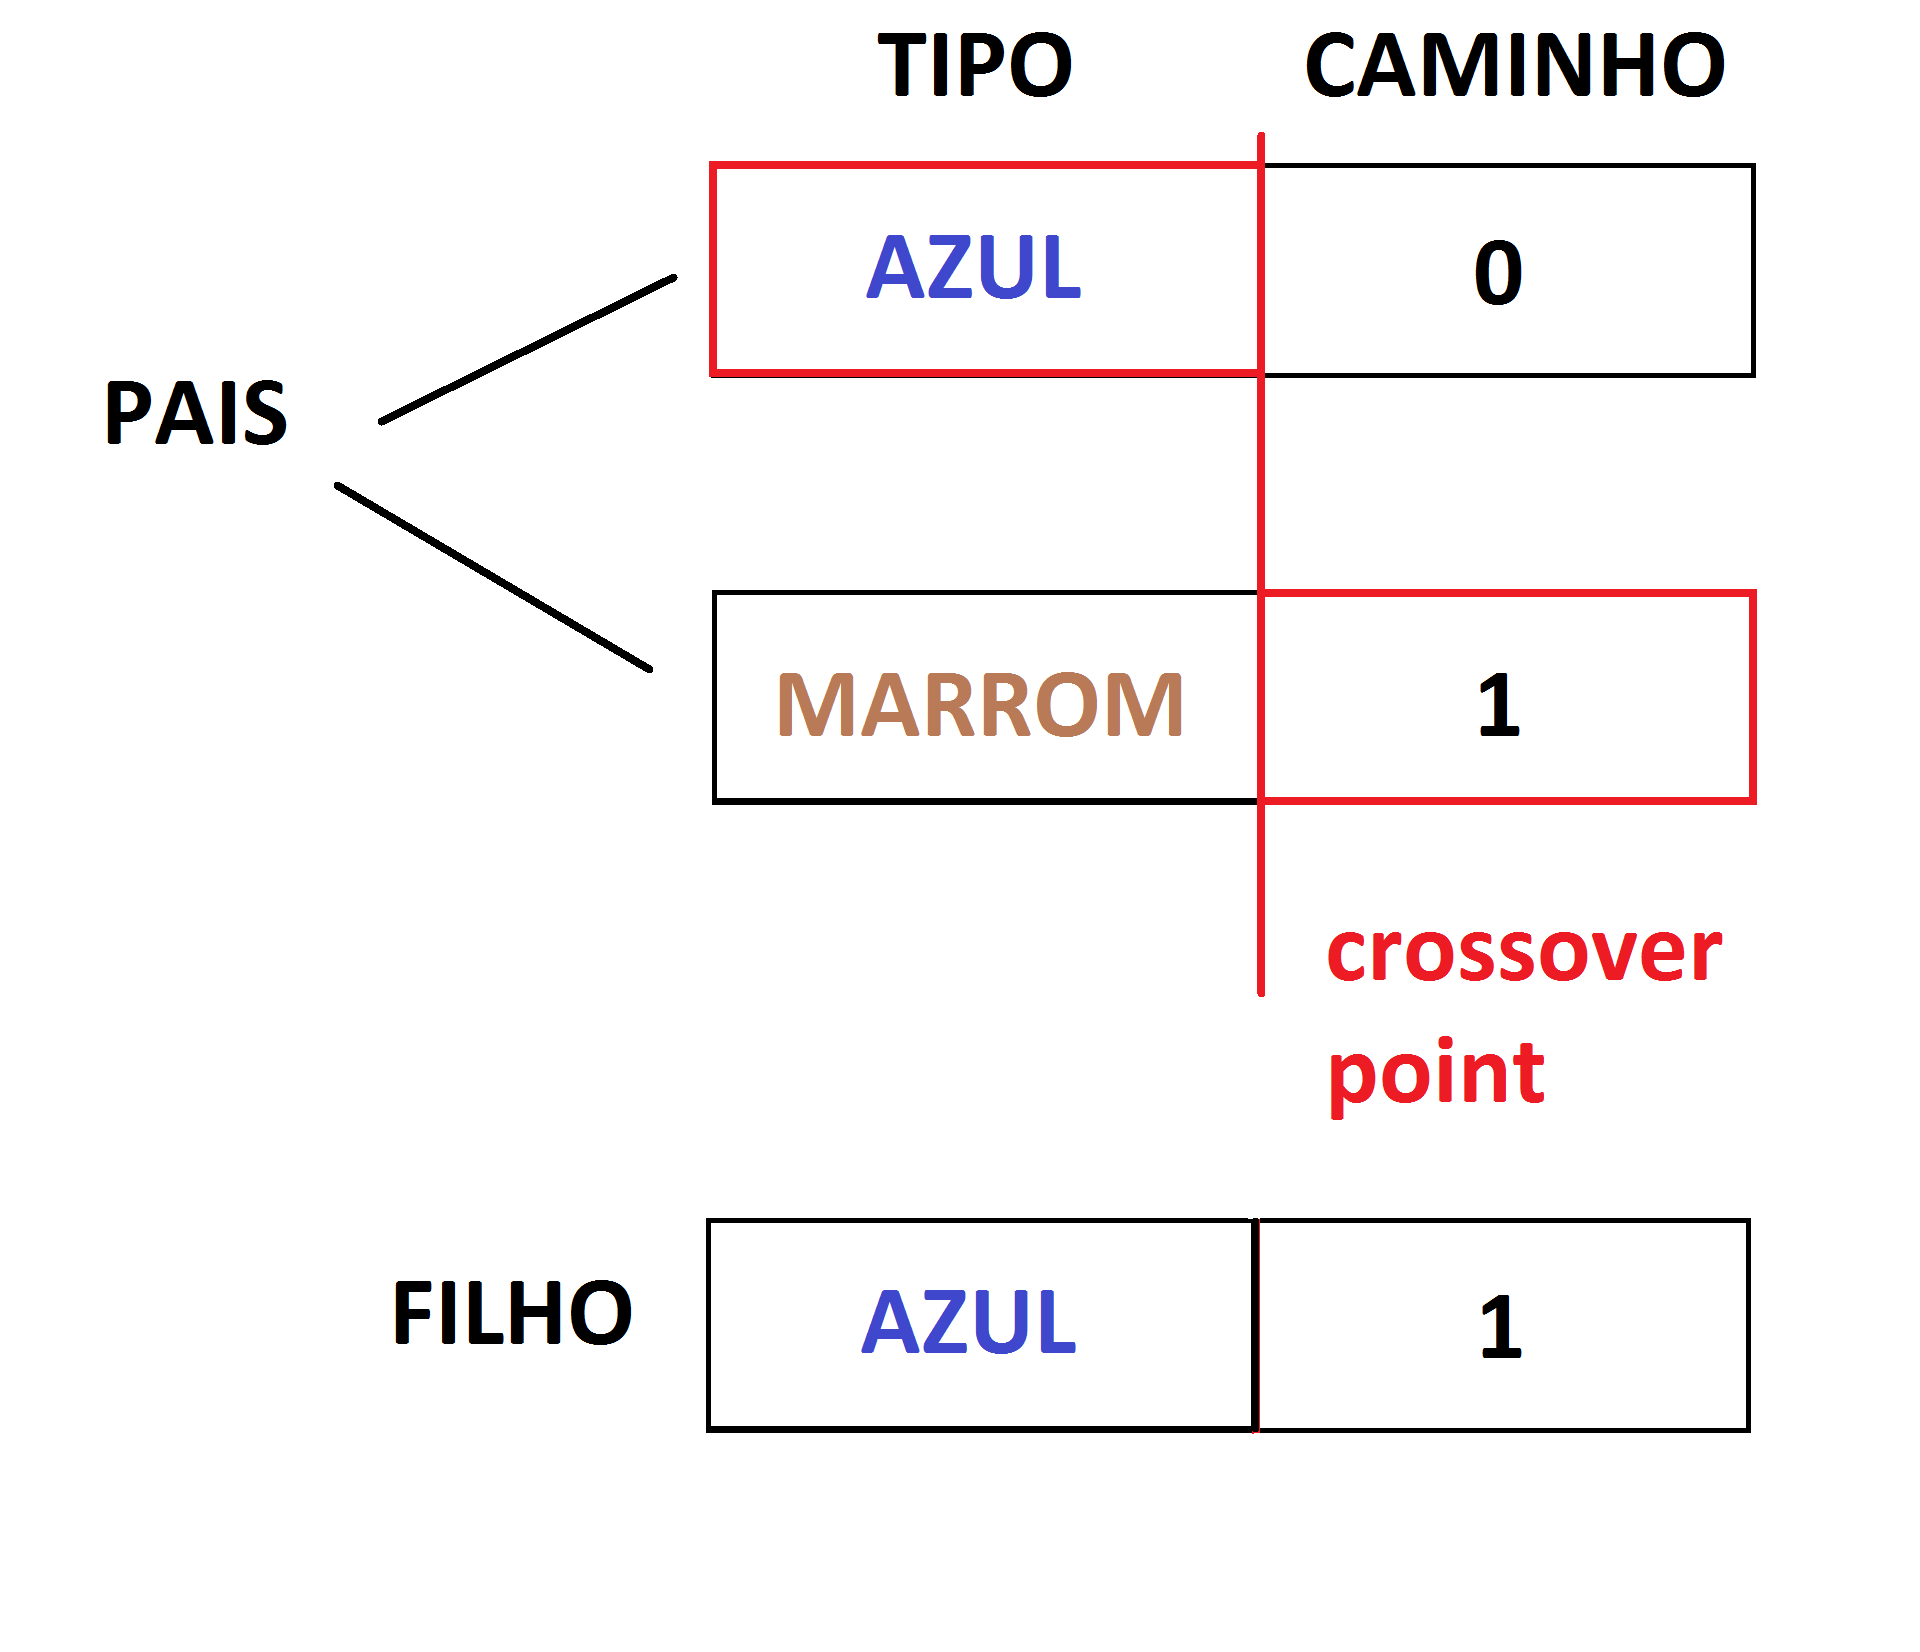
\includegraphics[width=.4\textwidth]{crossover}
  \caption{\textit{Crossover} para o caso do TD.\label{fig:crossover}}
\end{figure}

%% ------------------------------------------------------------------------- %%
\subsection{Mutação}
\label{sec:ag-mutacao}

A mutação representa a parte do algoritmo que equilibra '\textit{exploitation vs exploration}', ou seja, o quanto o algoritmo deve continuar buscando novas soluções (\textit{exploration}) ou o quanto ele deve continuar tirando vantagem da solução que já encontrou (\textit{exploitation}). No caso do algoritmo genético implementado, a mutação pode ocorrer em um único gene de um ou mais indivíduos da população, adicionando variabilidade ao resultado final. \citep{eiben98:exploitvsexplore}. 

No caso do trabalho, como os testes tinham rigor mais determinístico (pela implementação), era esperado que a população final convergisse para algum resultado. Portanto, a taxa de mutação escolhida foi de $\frac{1}{\text{nº de individuos na pop}} = \frac{1}{12} ou \frac{1}{6}$. Uma taxa que pareceu adequada conforme o artigo de \citet{haupt00:mutationprob}.

\pagebreak

%% ------------------------------------------------------------------------- %%
\subsection{Atualização}
\label{sec:ag-atualizacao}

Os indivíduos resultantes serão adicionados na população na etapa de atualização  e, caso seja necessário, o processo descrito acontece novamente.

\begin{programruledcaption}{Resumo do código. \label{prog:resumo_AG}}
  \begin{lstlisting}[
    language={[brazilian]pseudocode},
    style=pseudocode,
    style=wider,
    functions={},
    specialidentifiers={},
  ]
    funcao start_experiment (pop) // Cria uma nova população baseada na população atual
        // Quantidade de pais para reprodução
        num_parents_mating := population.size() * 2 / 3
	
	    // Função de Avaliação dos pais mais aptos da população
	    fitness := cal_pop_fitness(population_res)
	
	    // Função de Seleção dos melhores candidatos para a reprodução
	    parents := select_mating_pool(population, fitness, num_parents_mating)
	
	    // offspring\_size [0] = quantidade de filhotes
	    // offspring\_size [1] = quantidade de genes
	    // length(pop) = quantidade de individuos em pop
	    // genes(pop) = quantidade de genes de qualquer individuo de pop
	    offspring_size := [length(pop) - parents.size(), genes(pop)]
	    
	    // Função de Cruzamento dos pais para gerar os filhos.
	    offspring_crossover := crossover (parents, offspring_size)

	    // Função de Mutação dos filhos
	    offspring_mutation := mutation (offspring_crossover)
	    
	    // Adiciona os pais que sobreviveram de volta no vetor população
	    para i = 0 até tamanho (parents):
		    new_population.append (parents[i])
		fim
		    
		// Adiciona a nova prole para a população
	    para i = 0 até tamanho (offspring_mutation):
		    new_population.append (offspring_mutation[i])
		fim

	    devolva new_population
    fim
  \end{lstlisting}
\end{programruledcaption}
\par

%!TeX root=../tese.tex
%("dica" para o editor de texto: este arquivo é parte de um documento maior)
% para saber mais: https://tex.stackexchange.com/q/78101/183146

%% ------------------------------------------------------------------------- %%


% Recomendação Will: mudar nome do cap para método de avaliação do algoritmo ou similar: X

% ao invés de usar delineamento usar design ou desenho: X

% colocar uma tabela ou imagem ilustrando o uso do quadrado latino no nosso trabalho: 

% colocar nota de rodapé em desenvolvimento primeiro paragrafo referente a ultimo acesso e URL site:X

% WILL : "Qual a diferença de atributos entre os diferentes tanques e torres mesmo? Acho que vocês mencionam antes no texto mas é bom repetir, mover para aqui, ou pelo menos referenciar a seção onde foi dito": X

% Mencionar figuras no texto: X

% Mencionar Tabelas no texto: X

% deixar mais claro que soluções ingenuas servem para ser comparadas com algoritmo genético.: X

% Figuras sempre com letra maiúscula quando for mencionar no texto:X



\chapter{Método de Avaliação do algoritmo}
\label{cap:testes}

Com o algoritmo funcional, foi necessário buscar maneiras de avaliar seu desempenho para garantir sua eficiência \textit{versus} inimigos gerados aleatoriamente. Foram consideradas as possibilidades de distribuir os jogos e coletar \textit{feedback} de outros jogadores, mas considerando possíveis avaliações subjetivas para os jogos relativamente simples e limitações de tempo decidiu-se por utilizar métodos automatizados para coleta de resultados de dano em sequências de ondas.

%% ------------------------------------------------------------------------- %%
\section{Metodologia}
\label{sec:t-metodologia}

Segundo o Teorema Central do Limite, são necessárias, no mínimo, 30 amostras para que a média das mesmas tenha uma distribuição aproximadamente normal \citep{Magalhaes_estatistica}. Portanto, foram planejados experimentos nos jogos para geração de 30 amostras de dados em cada modo de jogo, para produção de gráficos com o comportamento das ondas, e desenho em quadrado latino.

%% ------------------------------------------------------------------------- %%
\subsection{Quadrado Latino}
\label{sec:t-quad-latino}

A coleta e disposição dos dados teve como objetivo a montagem de um quadrado latino.
Um quadrado latino de v linhas por v colunas é um arranjo de v letras latinas na forma de uma tabela, de maneira que cada letra ocorra apenas uma vez em cada linha, e uma vez em uma coluna, \citep{Design_exp_latin_sq}. Por exemplo, a tabela 3 x 3 é um quadrado latino:

\begin{table}
\caption{Exemplo de quadrado latino}
\begin{tabular}{ccc}
    A       & B    & C     \\ 
    B       & C    & A     \\
    C       & A    & B      \\
\end{tabular}
\end{table}

O desenho em quadrado latino é usado em experimentos onde os objetos de estudo estão submetidos a uma series de tratamentos, onde o tempo decorrido terá influência significativa nas respostas \citep{Design_exp_latin_sq}. A escolha do desenho em quadrado latino também é apropriada dado que os ambientes em que os testes foram feitos não são exatamente iguais, e por existirem dois fatores que podem influenciar nas respostas\citep{campbell:quadradolatino} - a inteligência artifical e o jogador que está sendo simulado.


%% ------------------------------------------------------------------------- %%
\section{Experimentos com o Algoritmo}
\label{sec:t-testes-algoritmo}

Durante o decorrer dos experimentos, notou-se incoerências nos testes realizados pelos códigos produzidos. Em especial, na função \textit{fitness} e na taxa de mutação.

\subsection{Fitness}

A função de avaliação (\textit{fitness}) é passada pelo usuário do código e, portanto, tiveram que ser criadas. No próximo capítulo \ref{sec:a-fitness}, será explicado mais detalhadamente sobre os resultados produzidos com diferentes funções de avaliação (\textit{fitness}) e as tentativas de alcançar outros resultados com base nelas.

\subsection{Taxa de mutação}

A taxa de mutação também pode ser definida pelo  usuário. Em particular, para testes pequenos como os feitos neste trabalho, é recomendado um valor entre $5\%$ até $20\%$. \citep{haupt00:mutationprob}.

Uma diferente abordagem ainda nesse tópico, é a utilização de taxas de mutação que decrescem conforme o tempo. Possui seus benefícios em testes de natureza mais determinística, já que espera-se que o algoritmo chegue em um ponto de convergência nas populações finais. Este método proporciona maior \textit{exploration} nas gerações iniciais, uma vez que está buscando o melhor resultado sem se prender em pontos de máximo local e maior \textit{exploitation} nas gerações finais, pois estará explorando o melhor resultado que obteve até o momento. \citep{eiben98:exploitvsexplore}

%% ------------------------------------------------------------------------- %%
\section{Desenvolvimento}
\label{sec:t-desenvolvimento}

Para fazer a coleta dos dados de maneira mais eficiente, os jogos foram adaptados para armazenarem os resultados das ondas. Foram desenvolvidas cenas no \textit{Godot} (menus e fases de teste), como pode se ver nas Figuras \ref{fig:tela-de-teste-tower defense} e \ref{fig:tela-de-teste-space-shooter}, que executam os testes de maneira determinística e consistente, sem aceitar \textit{input} do jogador. O botão \textit{Test Mode} acessa a interface de testes, enquanto o botão \textit{Play Defaut mode} utiliza o modo de jogo padrão. Todos os resultados são gravados em arquivos ".txt" com nome e formatação pré-definidos para facilitar a análise exploratória dos dados em \textit{Jupyter Notebook} \footnote{ \url{https://github.com/raktanaka/tcc-results} - 21/12/2021}.

\pagebreak

\begin{figure}
  \centering
  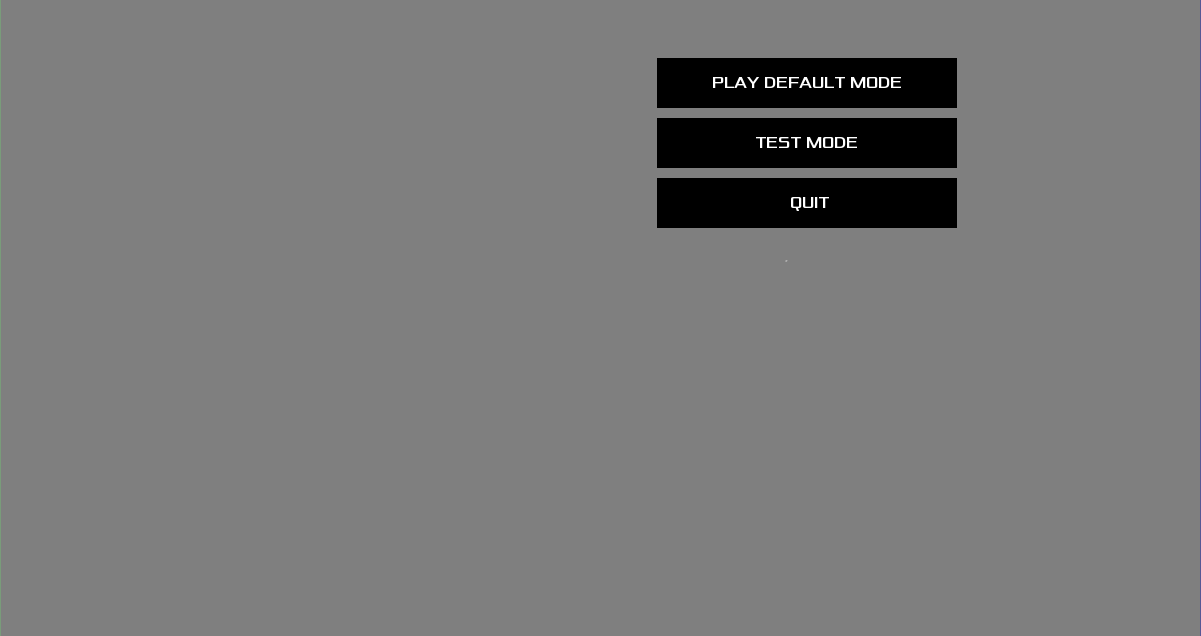
\includegraphics[width=.8\textwidth]{td/Tela_Teste_TDD.png}
  \caption{Tela de Teste Tower defense. Imagem retirada do próprio jogo.\label{fig:tela-de-teste-tower defense}}
\end{figure}

\begin{figure}
  \centering
  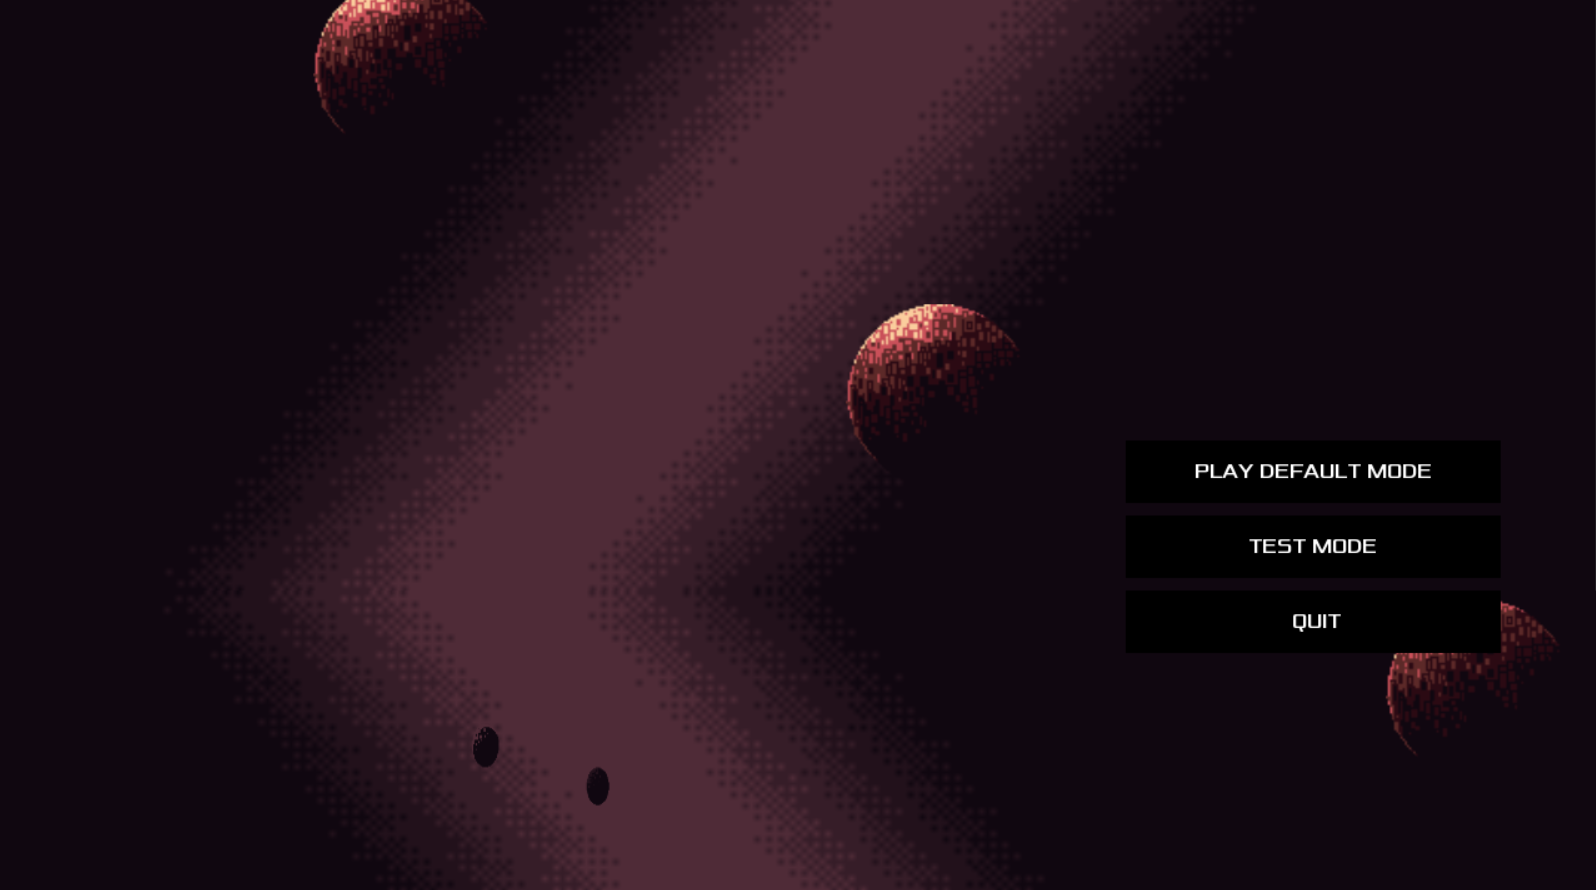
\includegraphics[width=.8\textwidth]{ss/Menu_SS.png}
  \caption{Tela de Teste Space Shooter. Imagem retirada do próprio jogo.\label{fig:tela-de-teste-space-shooter}}
\end{figure}


O menu \textit{Test Mode} permite escolher as configurações necessárias para a execução de um teste, com condições específicas e pré-definidas para obtenção de dados sobre as ondas geradas e o dano total produzido, o menu \textit{Test Mode} de cada jogo encontram-se nas Figuras \ref{fig:td-testes} e  \ref{fig:ss-testes}.

O algoritmo genético foi testado (opção \textit{AI} no menu), em conjunto com opções ingênuas nos dois jogos, posto que foram implementadas para ser comparadas com as ondas geradas pelo algoritmo desenvolvido, em vista de observar se seu desempenho. Assim há opções, apresentadas nas Figuras \ref{fig:td-testes} e \ref{fig:ss-testes} onde as ondas podem ser geradas:
\begin{itemize}
  \item Aleatoriamente - \textit{RANDOM}
  \item Um de cada oponente - \textit{ONE EACH}
  \item Modos "repetição", onde todo inimigo é do mesmo tipo
\end{itemize}

\begin{figure}
  \centering
  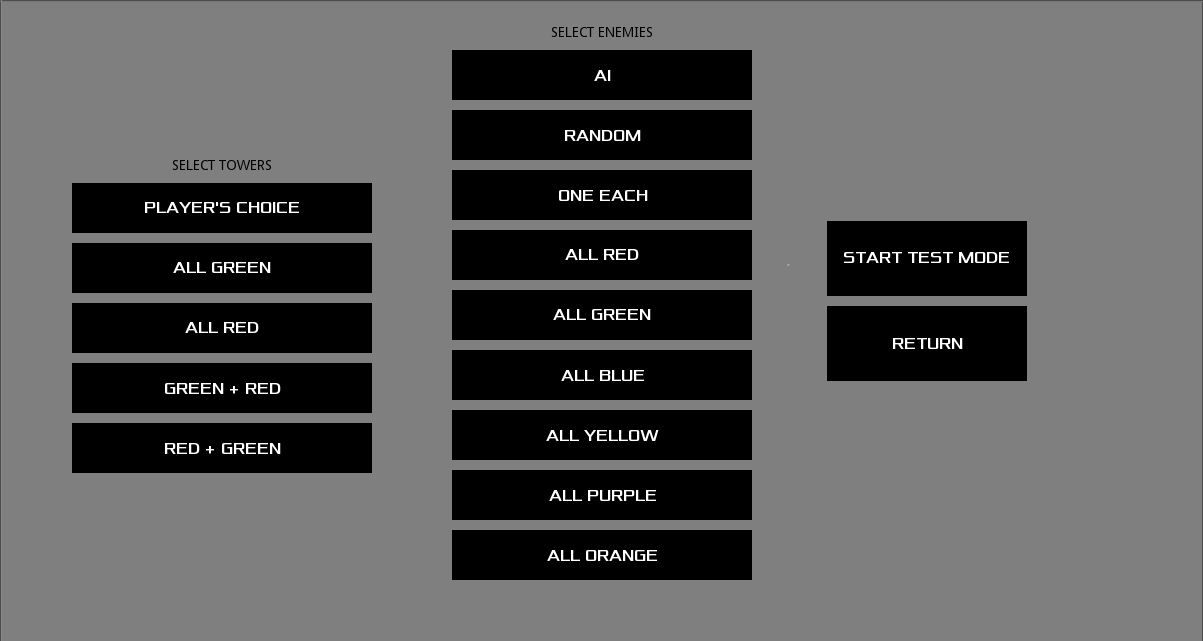
\includegraphics[width=.8\textwidth]{figuras/td/Menu_Escolhas_TESTE_TDD.PNG}
  \caption{Menu de testes Tower Defense. Imagem retirada do próprio jogo.\label{fig:td-testes}}
\end{figure}


\begin{figure}
  \centering
  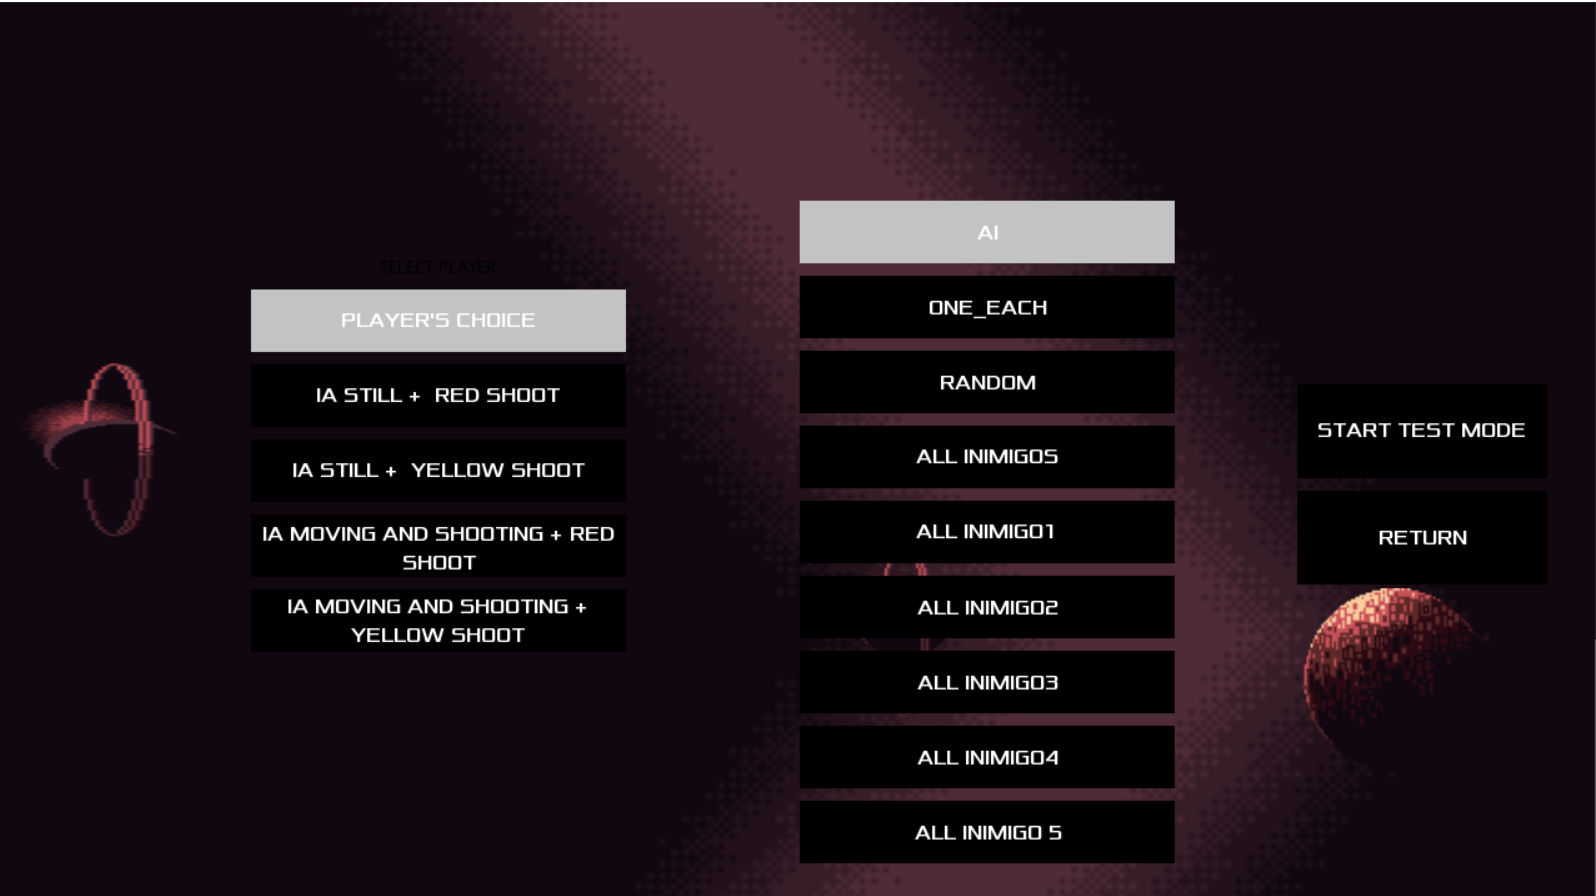
\includegraphics[width=.9\textwidth]{ss/Tela de testes_SS.png}
  \caption{Menu de Testes Space Shooter. Imagem retirada do próprio jogo.\label{fig:ss-testes}}
\end{figure}

\pagebreak

%% ------------------------------------------------------------------------- %%
\subsection{Tower Defense}
\label{sec:mt-td}

No \textit{Tower Defense}, as ondas repetidas enviam 6 inimigos iguais para cada rota norte e sul, um exemplo de uma onda repetida encontra-se na Figura \ref{fig:td-testes-orange} seguindo as rotas que foram já definidas conforme a Figura \ref{fig:td-rota}. Cada onda repetida envia o mesmo tipo de tanque, cujos atributos estam disponíveis na Tabela \ref{tab:tank-dmg2}. O modo \textit{One Each} utiliza os 6 tipos em cada rota; e o \textit{Random} aleatoriza completamente a escolha de tipo e rota, utilizando \textit{RandomNumberGenerator} disponibilizada pela \textit{Godot Engine}. Os modos \textit{Random} e \textit{One Each} podem ser vistos nas Figuras \ref{fig:tdd-testes} e \ref{fig:td-testes-one-each}. 


\begin{figure}
  \centering
  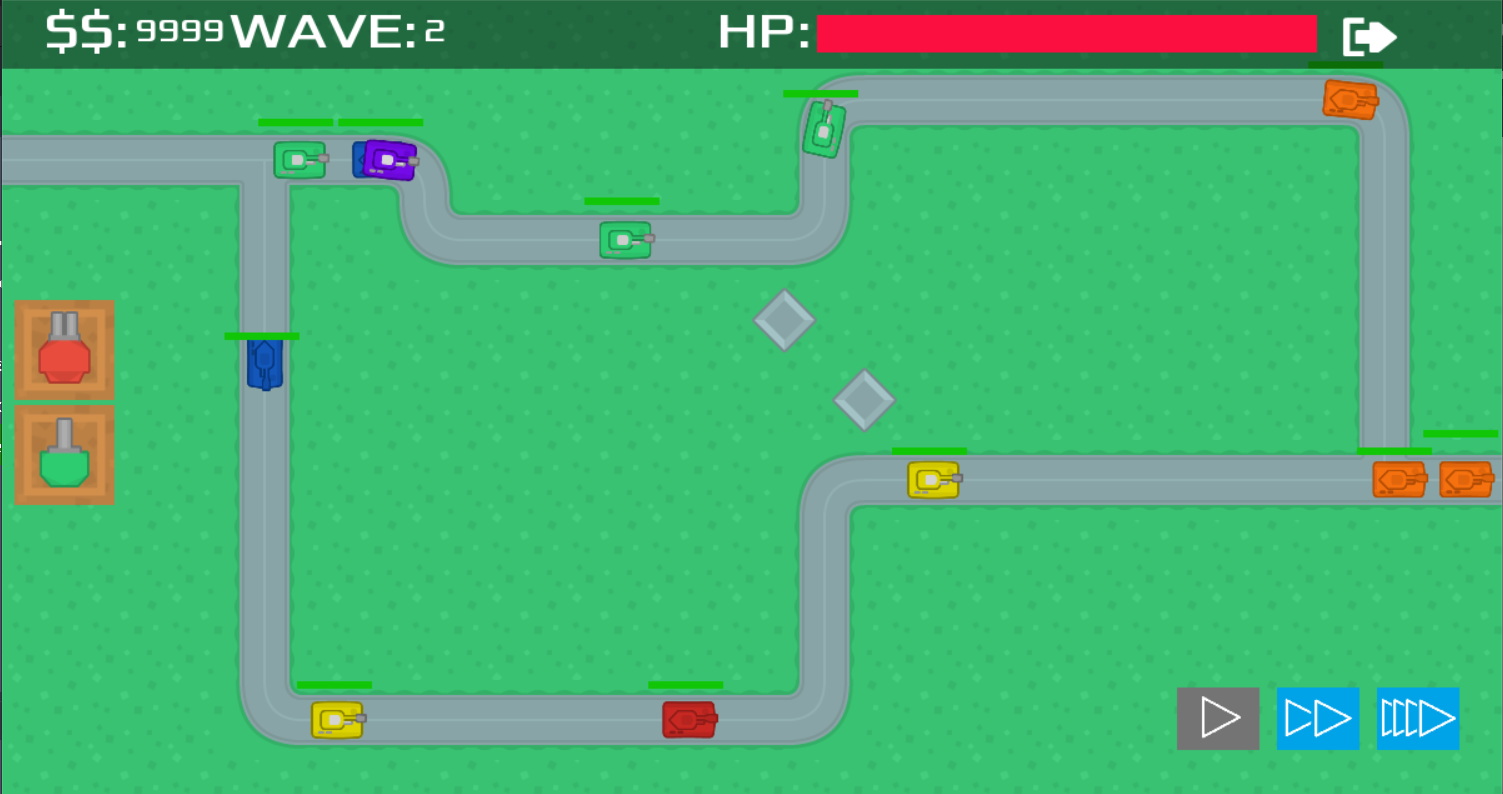
\includegraphics[width=.9\textwidth]{td/Random Mode_TDD Teste.PNG}
  \caption{Escolha Random em tower defense. Imagem retirada do próprio jogo.\label{fig:tdd-testes}}
\end{figure}


\begin{figure}
  \centering
  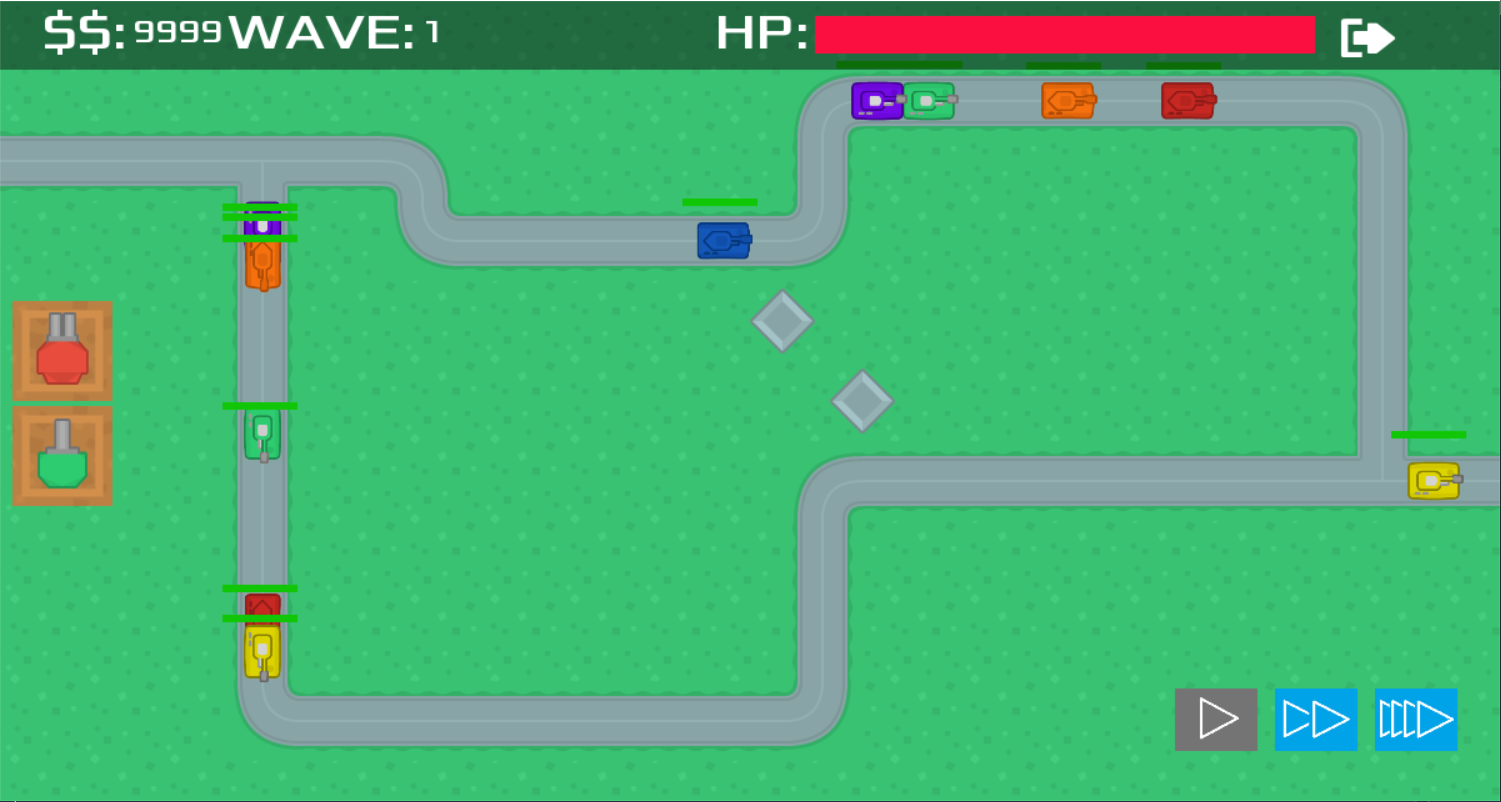
\includegraphics[width=.9\textwidth]{td/Exempleo TDD One EACH.PNG}
  \caption{Escolha One Each no Tower Defense. Imagem retirada do próprio jogo.\label{fig:td-testes-one-each}}
\end{figure}


\begin{figure}
  \centering
  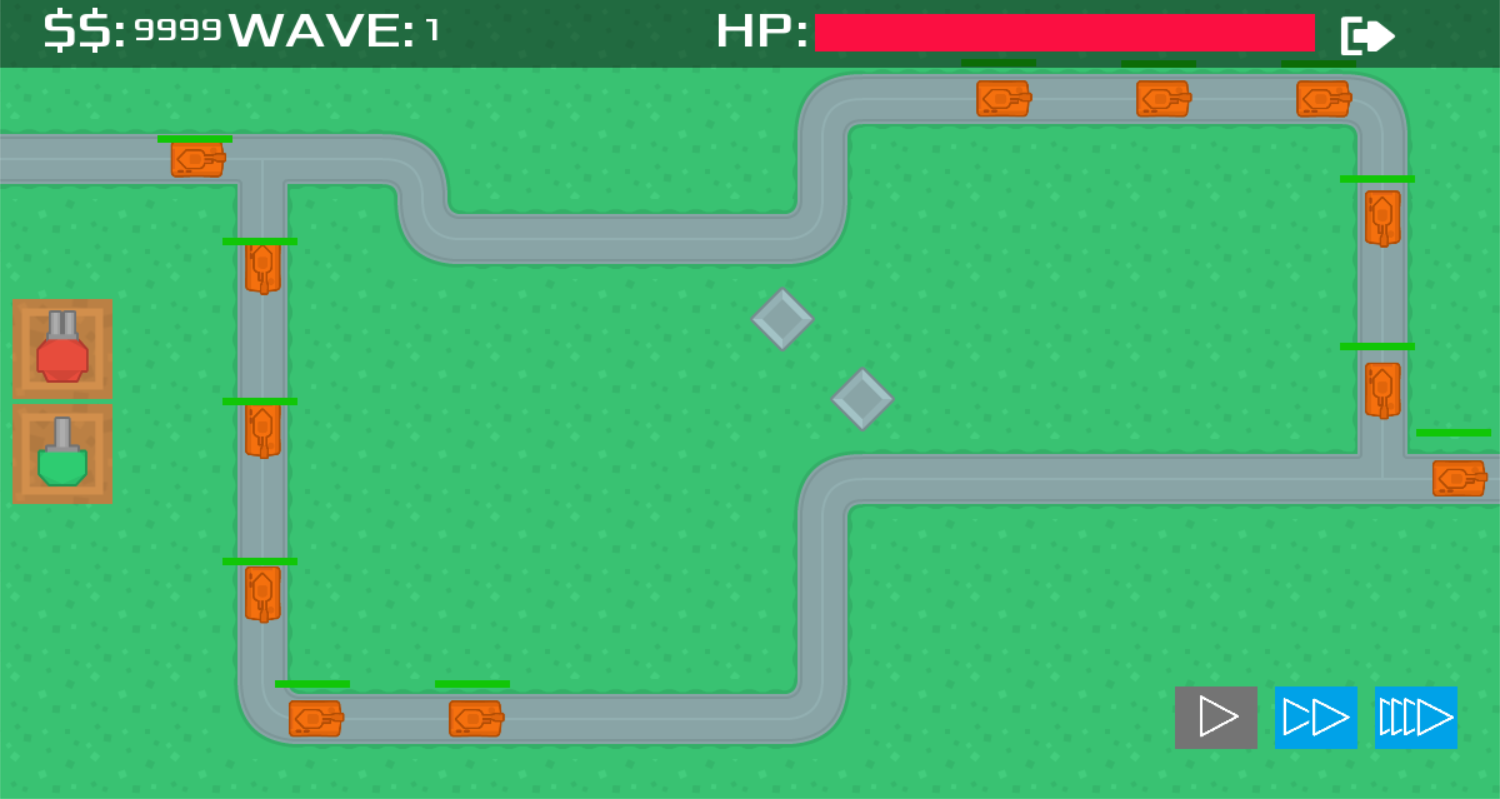
\includegraphics[width=.9\textwidth]{td/Tdd_All_orange.PNG}
  \caption{Opção All Orange. Imagem retirada do próprio jogo.\label{fig:td-testes-orange}}
\end{figure}

\pagebreak

Para uniformizar o comportamento do jogador, as torres foram configuradas para melhor controle dos testes, posicionadas duas por rota, onde o alcance das mesmas fica restrito a somente seu caminho, de maneira a alcançar um balanço entre eliminação e sobrevivência de alguns oponentes, visto as torres terem diferentes valores atribuídos com relação a dano e alcance, presentes na Tabela \ref{tab:dados_torres2}. Assim são geradas 4 configurações de teste, demonstradas nas Figuras \ref{fig:td-teste-all-green}, \ref{fig:tdd-teste-all-red}, \ref{fig:tdd-teste-greenred}, \ref{fig:td-teste-red-green}.

\begin{table}
\caption{Dano das torres no Tower Defense.\label{tab:dados_torres2}}
\begin{tabular}{c|ccc}

             & velocidade de tiro  & dano & alcance\\ \hline
Torre Verde   & 55     & 25     &  350 \\
Torre Vermelha     & 70     & 15     &  550       

\end{tabular}
\end{table}


\begin{table}
\caption{Dano de cada tanque no Tower Defense}
\begin{tabular}{c|cc}
            & velocidade & dano   \\ \hline
tank blue   & 55    & 55         \\
tank green  & 70    & 45         \\
tank red    & 80    & 15          \\
tank orange & 120   & 5           \\
tank purple & 90    & 15          \\
tank yellow & 150   & 5           
\end{tabular}
\label{tab:tank-dmg2}
\end{table}

\pagebreak

\begin{figure}
  \centering
  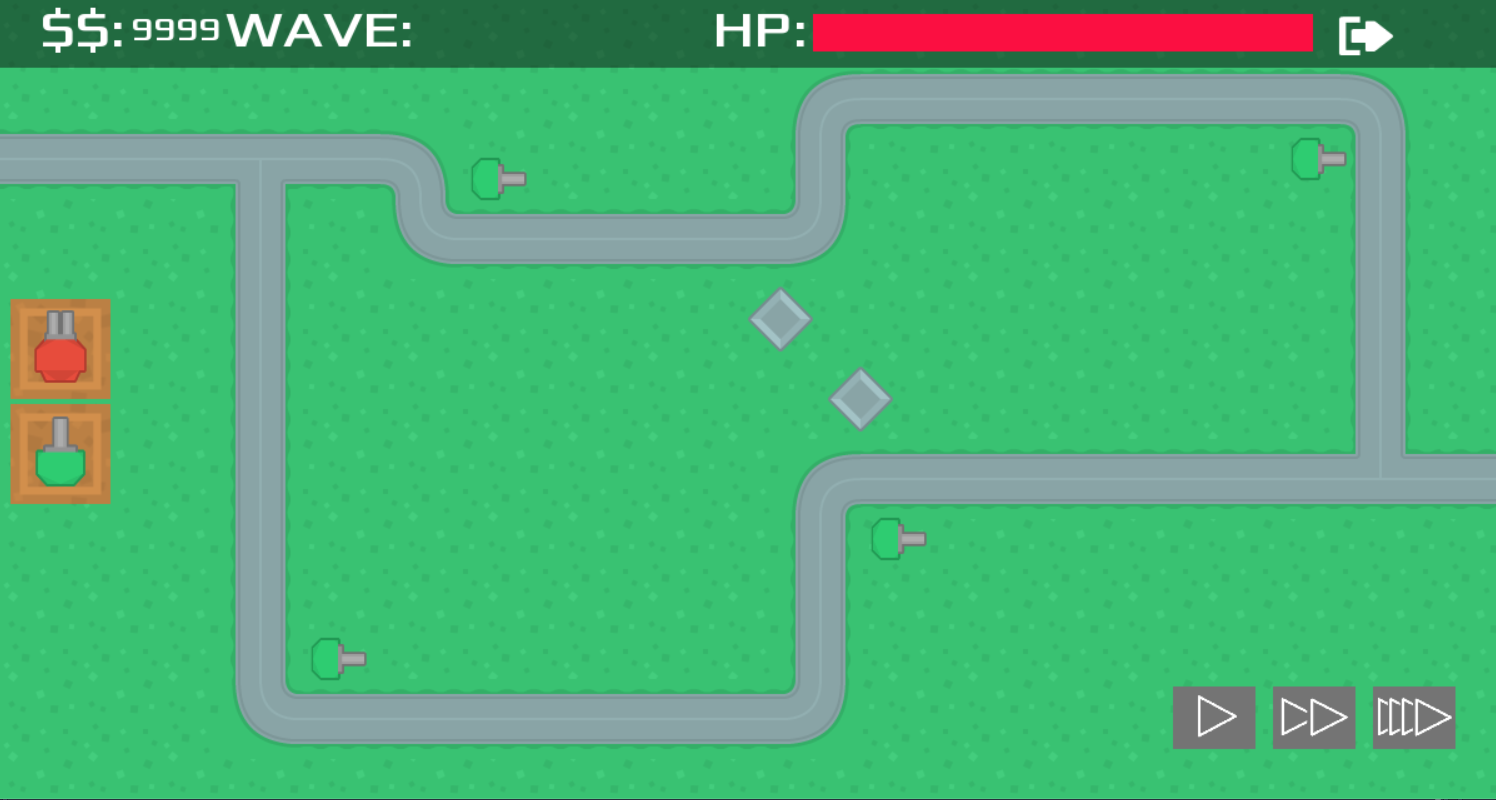
\includegraphics[width=.9\textwidth]{td/Tdd_all_green_teste.png}
  \caption{Teste de torres verdes\label{fig:td-teste-all-green}}
\end{figure}

\begin{figure}
  \centering
  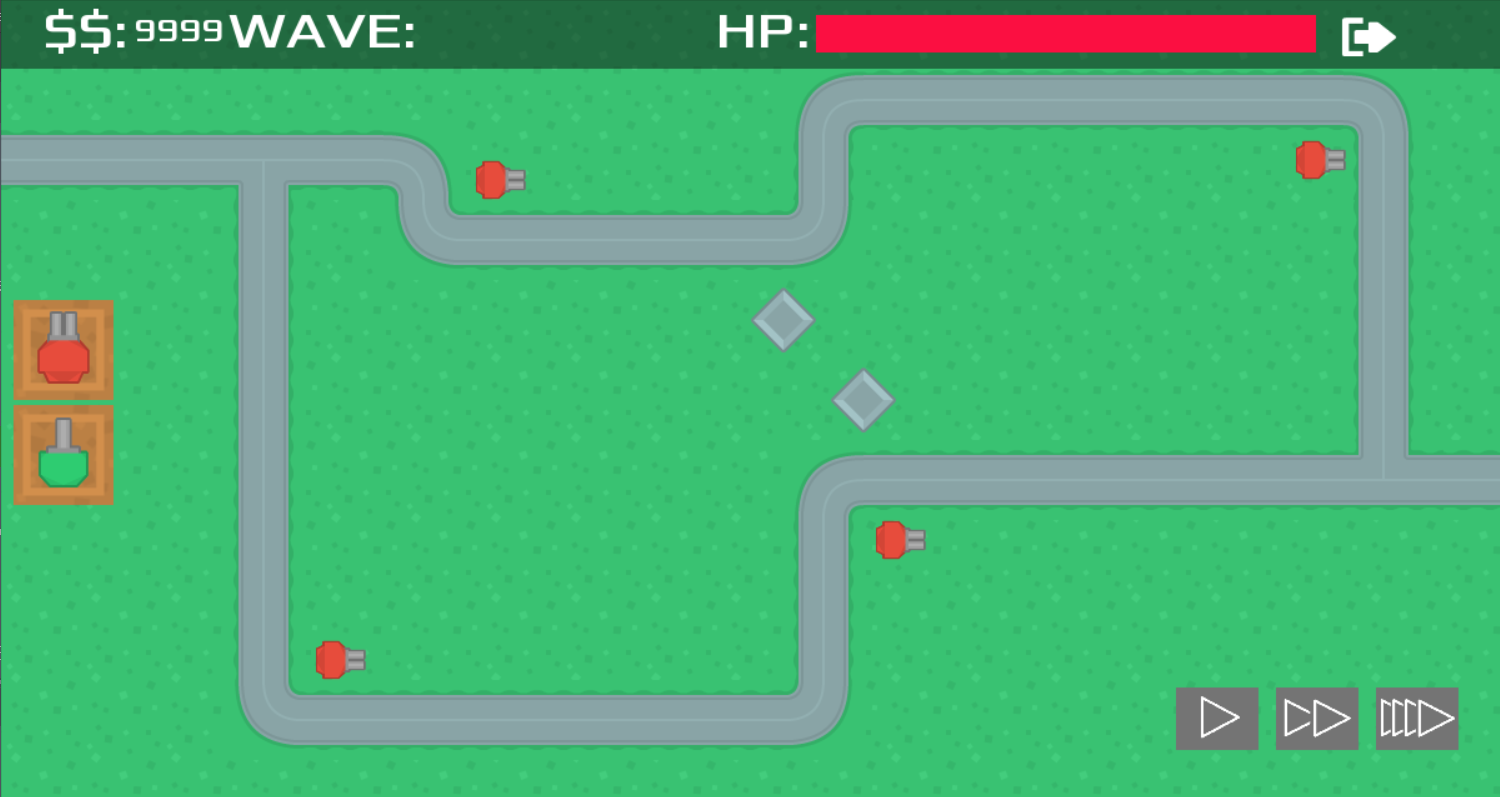
\includegraphics[width=.9\textwidth]{td/ALL RED TDD.png}
  \caption{Teste de torres vermelhas\label{fig:tdd-teste-all-red}}
\end{figure}

\begin{figure}
  \centering
  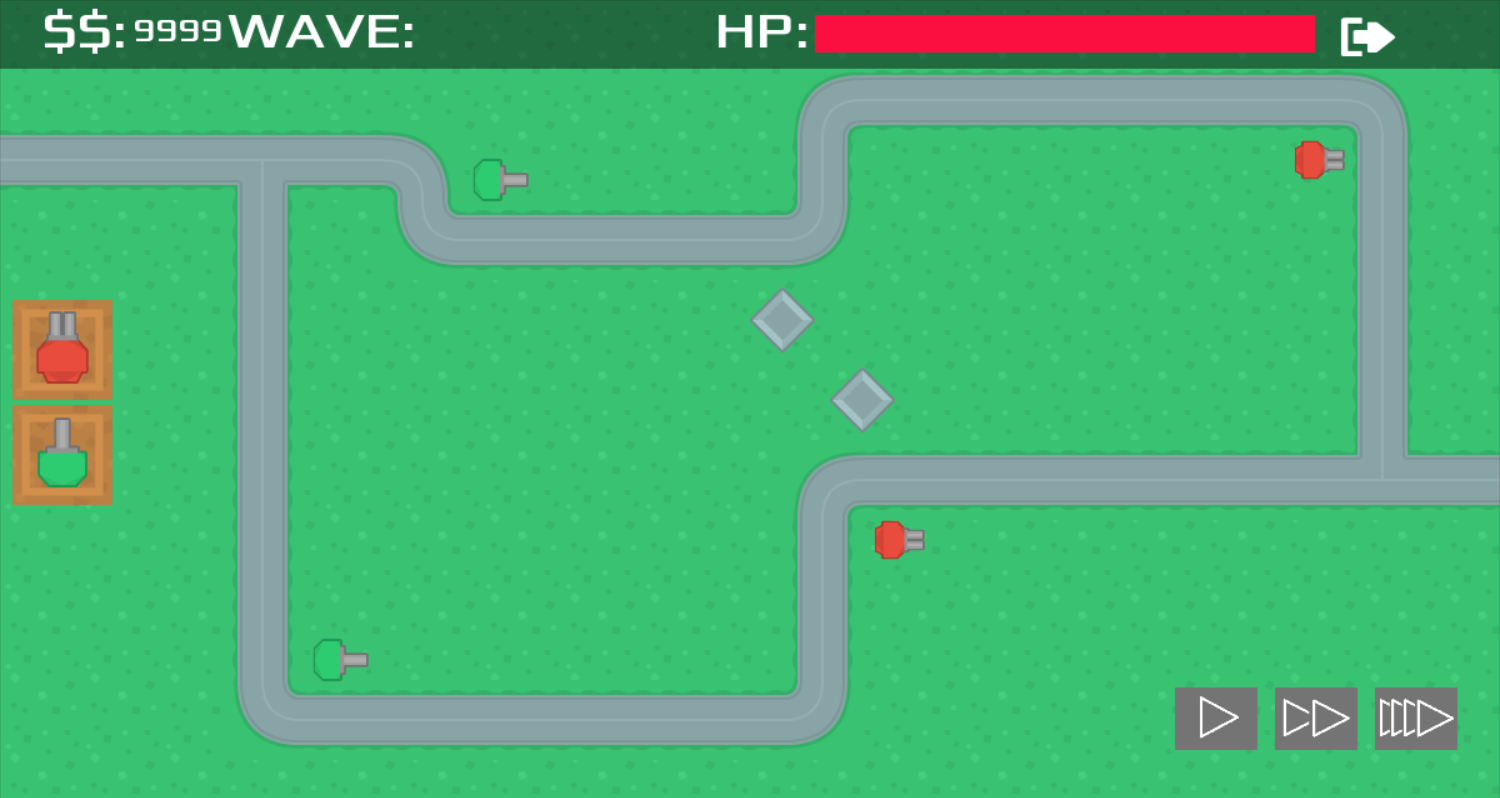
\includegraphics[width=.9\textwidth]{td/Green_Red_TDD.png}
  \caption{Teste de torres verdes com vermelhas\label{fig:tdd-teste-greenred}}
\end{figure}

\begin{figure}
  \centering
  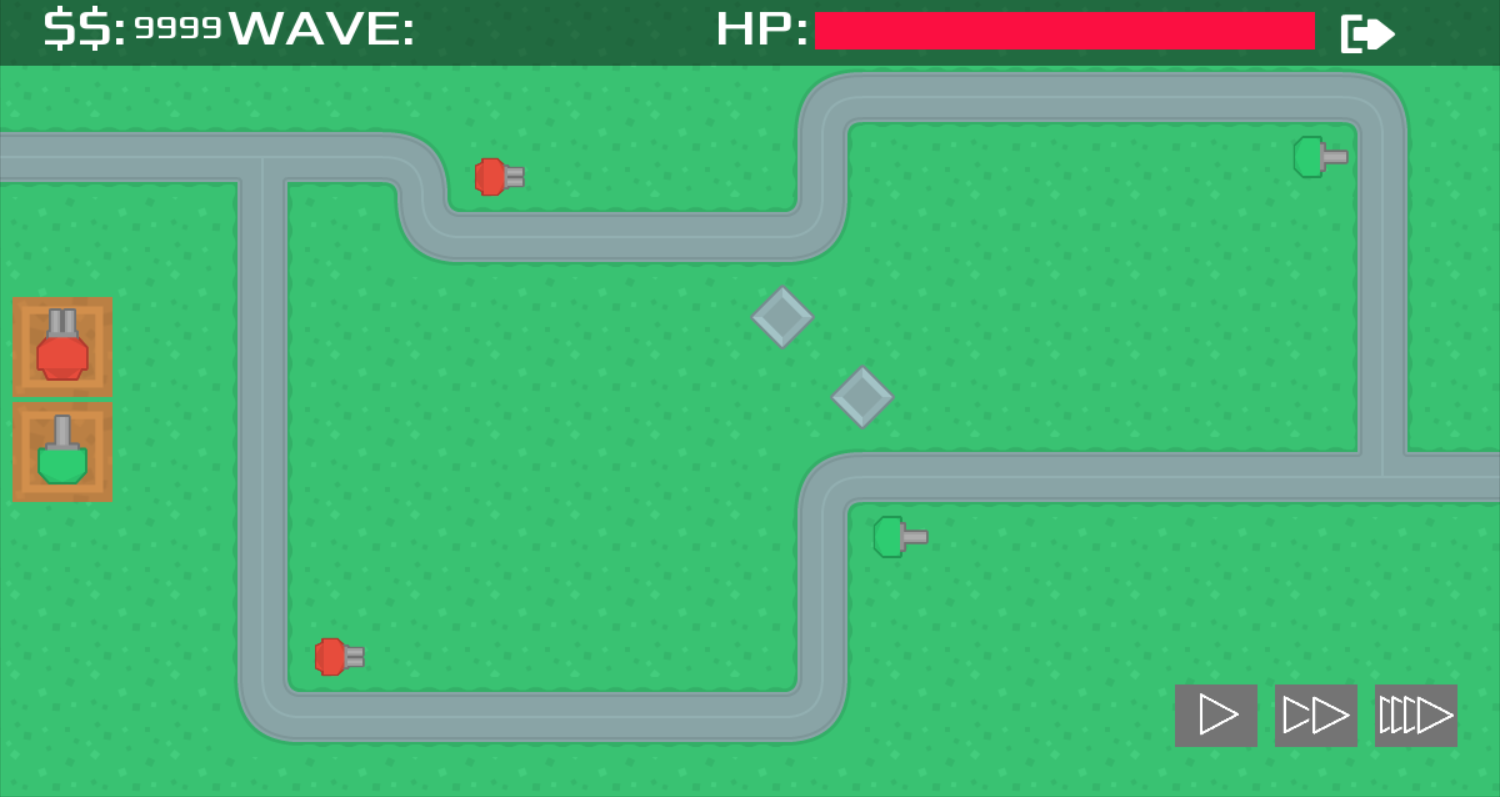
\includegraphics[width=.9\textwidth]{td/RED_GREEN TDD.png}
  \caption{Teste de torres vermelhas com verdes\label{fig:td-teste-red-green}}
\end{figure}

\newpage
%% ------------------------------------------------------------------------- %%
\subsection{Space Shooter}
\label{sec:mt-ss}

O \textit{Space Shooter} foi configurado de maneira próxima do \textit{Tower Defense}, mas foi preservada a capacidade dos asteroides aparecerem em locais aleatórios entre os 6 possíveis do jogo, exceto quando a IA está gerando os inimigos, onde o algoritmo busca o melhor \textit{spawn}. As naves foram alteradas para efetivamente jogarem a partida; com um nó \textit{Area2D} ao seu redor para detecção e ataque contra o primeiro inimigo que colidir contra o nó, conforme a Figura \ref{fig:ss-area}; e com a implementação de uma opção de movimentação, visto a Figura \ref{fig:ss-move}, permitindo testes com uma nave estática no centro da tela, e com movimentação lateral, de lado a lado, pausando nas extremidades.

\begin{figure}
  \centering
  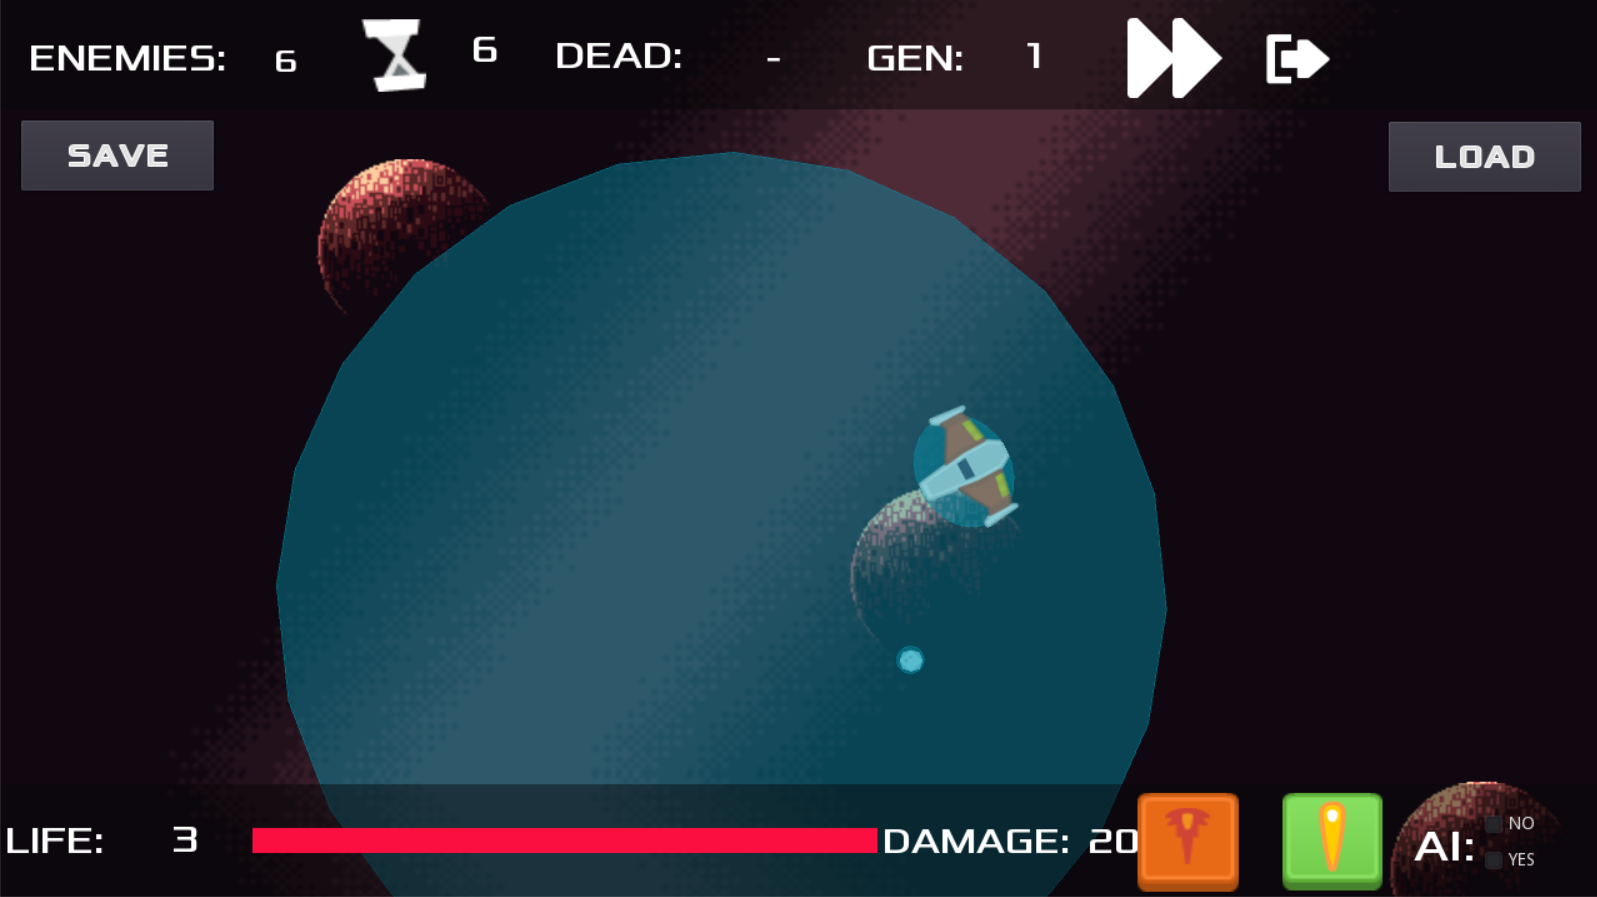
\includegraphics[width=.9\textwidth]{ss/Area de deteccao_Player_IA_jogo_exemplo.png}
  \caption{Área de detecção da nave em um modo de teste. Imagem retirada do próprio jogo.\label{fig:ss-area}}
\end{figure}

\begin{figure}
  \centering
  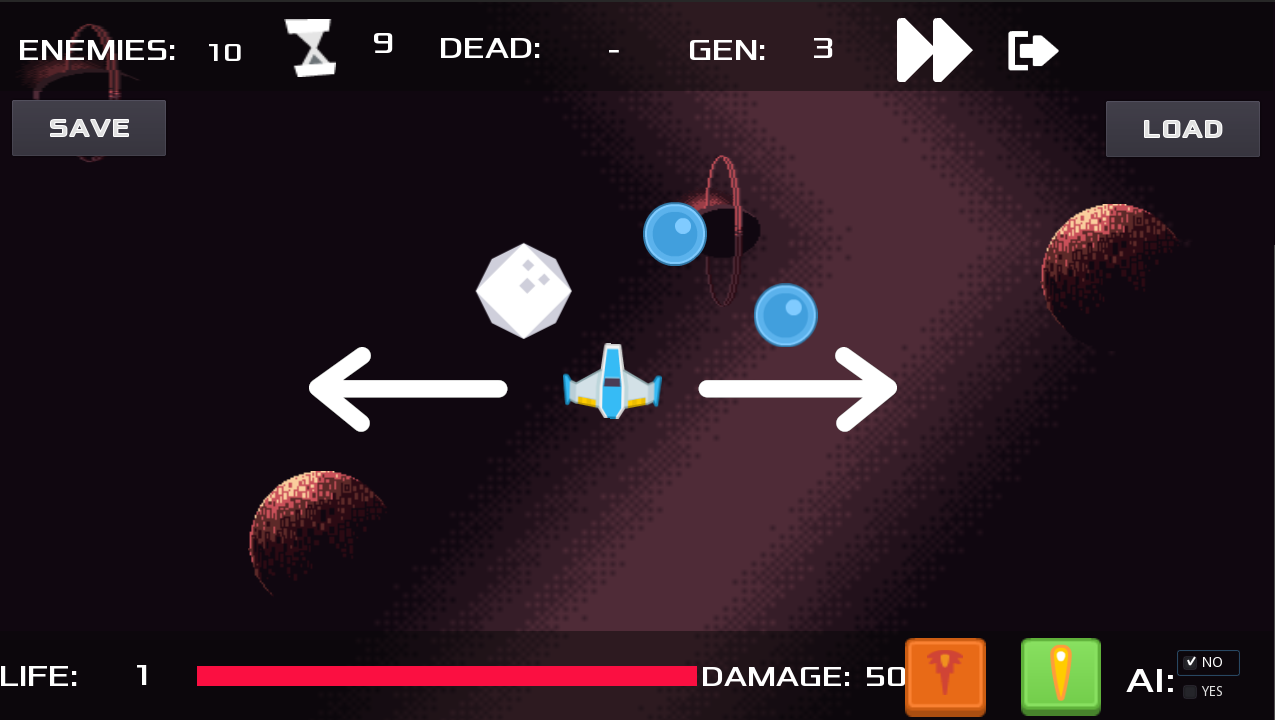
\includegraphics[width=.9\textwidth]{ss/ss_move.png}
  \caption{Movimentação da nave em um modo de teste. Imagem retirada do jogo e editada.\label{fig:ss-move}}
\end{figure}

\pagebreak

As opções dos inimigos são semelhantes ao \textit{Tower Defense}, com ondas sempre com os mesmos inimigos, ou um de cada, ou escolhendo aleatoriamente através do \textit{RandomNumberGenerator} da \textit{engine}. Reiterando que nestes casos o \textit{spawn} dos asteroides ocorre em qualquer um dos 6 locais disponíveis na Figura \ref{fig:ss-positions} escolhidos de maneira aleatória pelo jogo.
\par

%!TeX root=../tese.tex
%("dica" para o editor de texto: este arquivo é parte de um documento maior)
% para saber mais: https://tex.stackexchange.com/q/78101/183146

%% ------------------------------------------------------------------------- %%
\chapter{Apresentação dos Resultados}
\label{cap:apresentacao}

Para determinar a efetividade do algoritmo genético, foram utilizados métodos estatísticos para comparar o desempenho do mesmo contra outros mecanismos de geração de oponentes. Para aproveitar melhor as características determinísticas do jogo \textit{Tower Defense}, os experimentos se concentraram no mesmo, pois a natureza mais aleatória do \textit{Space Shooter} produziu resultados mais difíceis de analisar e, infelizmente, não havia mais tempo disponível para ajustar os cenários e função \textit{fitness} ou taxa de mutação até encontrar resultados mais conclusivos.

%% ------------------------------------------------------------------------- %%
\section{Organização dos dados}
\label{sec:a-organizacao}

A análise dos dados partiu das estatísticas descritivas de cada onda para todos os experimentos executados, conforme ilustrado pela Tabela \ref{tab:colunas}; isto é, foram obtidos 30 amostras de dano para cada i-ésima onda.

\begin{table}
\caption{Forma de coleta dos dados de cada onda.}
\begin{tabular}{l|l|l|l|l|l|l}
\cline{2-6}
               & onda 1 & onda 2 & ... & onda n - 1 & onda n \\ \cline{2-6}
experimento 1  &        &        &     &            &         \\
experimento 2  &  dano  &  dano  &     &  dano      &  dano   \\
...            &  da    &  da    & ... &  da        &  da     \\
experimento 29 &  onda  &  onda  &     &  onda      &  onda   \\
experimento 30 &        &        &     &            &         \\ \cline{2-6}
\end{tabular}
\label{tab:colunas}
\end{table}

%% ------------------------------------------------------------------------- %%
\section{Dados das Ondas}
\label{sec:a-ondas}

As seções seguintes irão dispor os dados considerados relevantes para análise de desempenho do algoritmo, obtidos através da análise exploratória de dados pelos \textit{Jupyter Notebook}\footnote{Repositório disponível em \url{https://github.com/raktanaka/tcc-results} - 24/12/2021} desenvolvidos. Dados de ondas sempre com o mesmo tipo de inimigos - chamadas de ondas repetidas - podem mostrar uma possível solução maximal ou próxima dela, para a qual o algoritmo poderia convergir. Já os dados de ondas com inimigos escolhidos ao acaso - chamadas de ondas aleatórias - indicam um possível valor de dano mínimo, que seria atingido com um método que também não precisa de conhecimento das mecânicas de jogo e de informações sobre os inimigos disponibilizadas.

Para visualização do funcionamento dos algoritmos, foram geradas imagens com as modas\footnote{Valores mais frequentes em um conjunto de dados} das ondas geradas a partir dos arquivos de texto com os dados. Um \textit{notebook} faz os cálculo necessários e utiliza a biblioteca \textit{Matplotlib} para produzir a imagem com os \textit{sprites} e caminho ou localização do inimigo. As figuras fornecem os inimigos mais comuns em cada onda, mostrando para qual solução o algoritmo tende a convergir. Estas estão disponíveis nos apêndices \ref{sec:apend-moda-td-v1}, \ref{sec:apend-moda-td-v2}, \ref{sec:apend-moda-td-v3}, \ref{sec:apend-moda-ss-v1}, \ref{sec:apend-moda-ss-v3}.

%% ------------------------------------------------------------------------- %%
\subsection{Tower Defense - Ondas Repetidas}
\label{sec:uni-td}

Seguem os dados obtidos nos experimentos feito no jogo, para facilidade de leitura, uma cópia da tabela \ref{tab:tank-dmg} da seção \ref{sec:mj-td} está abaixo.

\begin{table}
\caption{Dano de cada tanque no Tower Defense}
\begin{tabular}{c|cc}
            & velocidade & dano   \\ \hline
tank blue   & 55    & 55         \\
tank green  & 70    & 45         \\
tank red    & 80    & 15          \\
tank orange & 120   & 5           \\
tank purple & 90    & 15          \\
tank yellow & 150   & 5           
\end{tabular}
\label{tab:tank-dmg3}
\end{table}

Através da Tabela \ref{tab:tank-dmg3} é possível calcular o dano máximo possível como produto dos 12 inimigos que podem ser gerados por \textit{wave} e do maior dano disponível:
\[12 * 55 = 660\]
Numa onda composta inteiramente por tanques verdes (\textit{EnemyGreen}), sem nenhuma eliminação. As Tabelas \ref{tab:green}, \ref{tab:red}, \ref{tab:greenred} e \ref{tab:redgreen} a seguir mostram os dados de dano médio para cada onda e cada tipo de inimigo, obtidos através das simulações do jogo.

\begin{table}
\caption{Desempenho das \textbf{ondas repetidas} contra Torres \textbf{exclusivamente Verdes}}
\begin{tabular}{l|l|ll}
Torres & Inimigos & Dano Médio & Desvio Padrão \\ \hline
Verdes & EnemyGreen    & 450.00     & 0.0           \\
Verdes & OneEach       & 122.35     & 4.52          \\
Verdes & EnemyPurple   & 90.06      & 0.91          \\
Verdes & EnemyRed      & 89.90      & 1.22          \\
Verdes & EnemyBlue     & 60.68      & 16.77         \\
Verdes & EnemyYellow   & 40.07      & 0.57          \\
Verdes & EnemyOrange   & 39.93      & 0.57         
\end{tabular}
\label{tab:green}
\end{table}

Conforme os dados gerados para torres exclusivamente verdes, nota-se que tanques verdes possuem maior facilidade em causar dano ao jogador, uma vez que possuem a mecânica de \textbf{Resistência} contra torres da mesma cor que eles. Portanto, no algoritmo genético, espera-se que esses sejam os indivíduos mais numerosos da população final.

\begin{table}
\caption{Desempenho das \textbf{ondas repetidas} contra Torres \textbf{exclusivamente Vermelhas}}
\begin{tabular}{l|l|ll}
Torres    & Inimigos & Dano Médio & Desvio Padrão \\ \hline
Vermelhas & EnemyGreen    & 360.00     & 0.0           \\
Vermelhas & EnemyBlue     & 355.85     & 28.58         \\
Vermelhas & EnemyRed      & 180.00     & 0.0           \\
Vermelhas & OneEach       & 167.82     & 2.48          \\
Vermelhas & EnemyPurple   & 127.60     & 8.54          \\
Vermelhas & EnemyYellow   & 50.58      & 1.61          \\
Vermelhas & EnemyOrange   & 50.00      & 0.0          
\end{tabular}
\label{tab:red}
\end{table}

Os dados gerados para torres exclusivamente vermelhas apresenta que, em média,  tanques Verdes e Azuis são os melhores causadores de dano por onda, mesmo com a resistência dos tanques vermelhos sobre as torres vermelhas. Essa disparidade ocorre pela quantidade de dano que os tanques causam ao chegar no inimigo, conforme Tabela \ref{tab:tank-dmg3}, o tanque vermelho causa 15 de dano, ou seja, os 12 ($\frac{180}{15}$) tanques sobrevivem ao final de todas as ondas. Contudo, os inimigos verdes e azuis causam mais dano, mesmo que cheguem menos tanques ao final do trajeto, 8 ($\frac{360}{45}$) para tanques verdes e entre 6-7 ($\frac{355}{55}$) nos azuis. 

\begin{table}
\caption{Desempenho das \textbf{ondas repetidas} contra \textbf{1 Torre Verde e 1 Vermelha} (Nessa ordem)}
\begin{tabular}{l|l|ll}
Torres           & Inimigos & Dano Médio & Desvio Padrão \\ \hline
Verde + Vermelha & EnemyGreen    & 420.20     & 13.91         \\
Verde + Vermelha & EnemyBlue     & 220.18     & 3.18          \\
Verde + Vermelha & EnemyRed      & 148.50     & 4.50          \\
Verde + Vermelha & OneEach       & 148.45     & 4.57          \\
Verde + Vermelha & EnemyPurple   & 120.00     & 0.0           \\
Verde + Vermelha & EnemyYellow   & 50.00      & 0.0           \\
Verde + Vermelha & EnemyOrange   & 44.50      & 1.50          
\end{tabular}
\label{tab:greenred}
\end{table}

\pagebreak

Conforme as informações da Tabela \ref{tab:greenred}, percebe-se que o inimigo Verde tem o melhor desempenho de dano por onda repetida, mesmo que sobrevivam menos indivíduos ao final em comparação ao inimigo Vermelho, uma vez que o dano de Verde é 3 vezes maior. Chegam ao final, aproximadamente 9 ($\frac{420}{45}$) Verdes e 10 Vermelhos ($\frac{148.5}{15}$). 

\begin{table}[H]
\caption{Desempenho das \textbf{ondas repetidas} contra \textbf{1 Torre Vermelha e 1 Verde}(Nessa ordem)}
\begin{tabular}{l|l|ll}
Torres            & Inimigos & Dano Médio & Desvio Padrão \\ \hline
Vermelha + Verde  & EnemyGreen      & 449.85     & 2.60          \\
Vermelha + Verde  & EnemyBlue       & 329.82     & 3.18          \\
Vermelha + Verde  & EnemyRed        & 149.90     & 1.73          \\
Vermelha + Verde  & OneEach         & 135.05     & 0.87          \\
Vermelha + Verde  & EnemyPurple     & 120.00     & 0.0           \\
Vermelha + Verde  & EnemyYellow     & 50.00      & 0.0           \\
Vermelha + Verde  & EnemyOrange     & 49.45      & 1.57          
\end{tabular}
\label{tab:redgreen}
\end{table}

Para a Tabela \ref{tab:redgreen}, nota-se um aumento de desempenho significativo do inimigo Azul e Verde, onde sobrevive um tanque a mais verde e quase 2 azuis em relação ao anterior. Contudo, mantém-se a dominância do dano médio por onda do inimigo Verde. Os desvios padrões baixos - o mais alto apresentado nas Torres Verdes contra \textit{EnemyBlue} é de aproximadamente 25\% do dano total, mas é uma exceção considerando todos os resultados - mostram a consistência do jogo.

Conforme os dados gerados, o inimigo Verde indica ter o melhor desempenho de dano nas ondas repetidas, contudo, mais para frente desse capítulo, será mostrado que eles não serão os mais selecionados, por conta da função \textit{fitness} escolhida, que prioriza sobrevivência ao invés de dano por \textit{wave}.

%% ------------------------------------------------------------------------- %%
\subsection{Tower Defense - Ondas Aleatórias}
\label{sec:rd-td}

Foram calculadas as médias de dano causadas por cada onda aleatória de distribuição uniforme (Tabela \ref{tab:td-rd-avg}) e o máximo de dano causado em qualquer onda (Tabela \ref{tab:td-rd-max}), considerando todos os experimentos. A Figura \ref{fig:td-rd-max} ilustra a onda que causou o maior dano.

\begin{table}
\begin{tabular}{l|ll}
Torres            & Dano Médio & Desvio Padrão \\ \hline
Verdes            & 81.42      & 55.00         \\
Vermelhas         & 125.35     & 56.98         \\
Verde + Vermelha  & 100.37     & 54.16         \\
Vermelha + Verde  & 102.37     & 56.62          
\end{tabular}
\caption{Média e Desvio Padrão do dano em ondas aleatórias no Tower Defense.}
\label{tab:td-rd-avg}
\end{table}

\pagebreak

\begin{table}
\centering
\begin{tabular}{p{1.7cm}|l|p{1.0cm}}
Torres                   & Onda                                                                                                                         & Dano \newline Total \\ \hline
Verdes                   & \begin{tabular}{@{}c@{}} {[}EnemyGreen, 1{]}; {[}EnemyGreen, 1{]}; {[}EnemyGreen, 0{]}; {[}EnemyRed, 1{]};     \\
                                                    {[}EnemyPurple, 0{]}; {[}EnemyGreen, 0{]}; {[}EnemyRed, 1{]}; {[}EnemyGreen, 0{]};    \\
                                                    {[}EnemyOrange, 0{]}; {[}EnemyGreen, 0{]}; {[}EnemyGreen, 0{]}; {[}EnemyRed, 0{]}     \end{tabular} & 290        \\ \hline
Vermelhas                & \begin{tabular}{@{}c@{}} {[}EnemyBlue, 0{]}; {[}EnemyRed, 0{]}; {[}EnemyBlue, 0{]}; {[}EnemyGreen, 0{]};       \\
                                                    {[}EnemyGreen, 1{]}; {[}EnemyRed, 1{]}; {[}EnemyBlue, 0{]}; {[}EnemyOrange, 1{]};     \\
                                                    {[}EnemyBlue, 0{]}; {[}EnemyYellow, 0{]}; {[}EnemyOrange, 0{]}; {[}EnemyYellow, 1{]}  \end{tabular} & 355        \\ \hline
Verde + \newline Vermelha & \begin{tabular}{@{}c@{}} {[}EnemyPurple, 0{]}; {[}EnemyBlue, 0{]}; {[}EnemyBlue, 0{]}; {[}EnemyBlue, 1{]};    \\
                                                     {[}EnemyRed, 0{]}; {[}EnemyGreen, 1{]}; {[}EnemyYellow, 0{]}; {[}EnemyRed, 1{]};     \\
                                                     {[}EnemyGreen, 1{]}; {[}EnemyGreen, 0{]}; {[}EnemyGreen, 0{]}; {[}EnemyYellow, 1{]}  \end{tabular} & 330        \\ \hline
Vermelha \newline + Verde & \begin{tabular}{@{}c@{}} {[}EnemyYellow, 0{]}; {[}EnemyBlue, 0{]}; {[}EnemyRed, 1{]}; {[}EnemyGreen, 0{]};    \\
                                                     {[}EnemyGreen, 1{]}; {[}EnemyRed, 1{]}; {[}EnemyGreen, 0{]}; {[}EnemyYellow, 0{]};   \\
                                                     {[}EnemyRed, 1{]}; {[}EnemyGreen, 0{]}; {[}EnemyGreen, 0{]}; {[}EnemyPurple, 1{]}    \end{tabular} & 315       
\end{tabular}
\caption{Ondas aleatórias com maior dano no Tower Defense.}
\label{tab:td-rd-max}
\end{table}

\begin{figure}
  \centering
  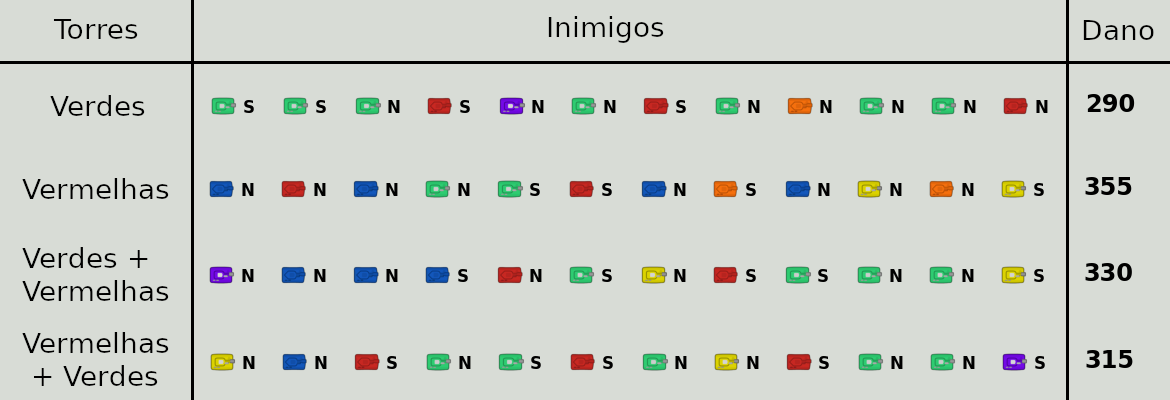
\includegraphics[width=1.0\textwidth]{td/tab-rd-max.png}
  \caption{Visualização das ondas aleatórias com maior dano no Tower Defense.}
  \label{fig:td-rd-max}
\end{figure}

%% ------------------------------------------------------------------------- %%
\subsection{Space Shooter - Ondas Repetidas}
\label{sec:uni-ss}


Foram executados experimentos análogos ao \textit{Tower Defense} no \textit{Space Shooter}, segue uma cópia da tabela \ref{tab:ss-ast-dmg} da seção \ref{sec:mj-ss} para facilitar leitura.

\begin{table}[H]
\caption{Velocidade, dano e vida de cada asteroide no Space Shooter}
\begin{tabular}{c|ccc}
         & Velocidade & Dano & Vida   \\ \hline
inimigos & 500        & 20     &   50     \\
inimigo1 & 350        & 45     &   30     \\
inimigo2 & 470        & 50     &   40     \\
inimigo3 & 320        & 60     &   40     \\
inimigo4 & 550        & 20     &   60     \\
inimigo5 & 700        & 10     &   120      
\end{tabular}
\label{tab:ss-ast-dmg-copia}
\end{table}

\pagebreak

Através da Tabela \ref{tab:ss-ast-dmg-copia}, é possível calcular o dano máximo possível como a onda de seis inimigos com o maior dano disponível:
\[6 * 60 = 360\]
Numa onda composta inteiramente pelo \textit{inimigo3}, sem nenhuma eliminação. As tabelas \ref{tab:ss-yellow-still}, \ref{tab:ss-yellow-move}, \ref{tab:ss-red-still} e \ref{tab:ss-red-move} a seguir mostram os dados de dano médio para cada onda e cada tipo de inimigo.

\begin{table}
\centering
\caption{\textbf{Ondas repetidas} contra IA de \textbf{Disparo Amarelo} e \textbf{Parado}} .
\begin{tabular}{l|l|ll}
Nave                     & Inimigo  & Dano Médio & Desvio Padrão \\ \hline
Disparo Amarelo - Parada & Inimigo3 & 314.93     & 42.46         \\
Disparo Amarelo - Parada & Inimigo2 & 299.78     & 3.33          \\
Disparo Amarelo - Parada & Inimigo1 & 181.50     & 41.67         \\
Disparo Amarelo - Parada & Inimigo4 & 120.00     & 0.0           \\
Disparo Amarelo - Parada & Inimigos & 120.00     & 0.0           \\
Disparo Amarelo - Parada & OneEach  & 82.75      & 27.47         \\
Disparo Amarelo - Parada & Inimigo5 & 60.00      & 0.0          
\end{tabular}
\label{tab:ss-yellow-still}
\end{table}

Na tabela, nota-se que os valores piores classificados são as ondas em que todos os asteroides chegaram no Jogador, mas possuem danos muito baixos ($\frac{\text{dano médio}}{\text{dano individual do asteróide}}$), enquanto os que possuem danos melhores perderam algum indivíduo da população no caminho, pois possuem valores menores que os danos totais possíveis (dano * 6, onde 6 é quantidade de inimigos) e seu desvio padrão é alto.

\begin{table}
\centering
\caption{\textbf{Ondas repetidas} contra IA de \textbf{Disparo Amarelo} e \textbf{Movendo}}.
\begin{tabular}{l|l|ll}
Nave                      & Inimigo  & Dano Médio & Desvio Padrão \\ \hline
Disparo Amarelo - Movendo & Inimigo3 & 213.20     & 52.43         \\
Disparo Amarelo - Movendo & Inimigo2 & 184.61     & 41.98         \\
Disparo Amarelo - Movendo & Inimigo1 & 130.10     & 48.15         \\
Disparo Amarelo - Movendo & OneEach  & 100.85     & 43.75         \\
Disparo Amarelo - Movendo & Inimigo4 & 80.69      & 15.70         \\
Disparo Amarelo - Movendo & Inimigos & 67.69      & 15.46         \\
Disparo Amarelo - Movendo & Inimigo5 & 39.23      & 7.71         
\end{tabular}
\label{tab:ss-yellow-move}
\end{table}

Para esses dados, nota-se que, com a Nave se movendo, a chance dos inimigos acertarem o Jogador decai bastante em todos os casos, contudo, os tipos de inimigos mais promissores ainda se mantém como Inimigo3, Inimigo2 e Inimigo1.

\pagebreak

\begin{table}
\centering
\begin{tabular}{l|l|ll}
Nave                      & Inimigo  & Dano Médio & Desvio Padrão \\ \hline
Disparo Vermelho - Parada & Inimigo3 & 241.60     & 56.01         \\
Disparo Vermelho - Parada & Inimigo2 & 240.94     & 56.09         \\
Disparo Vermelho - Parada & OneEach  & 125.99     & 38.03         \\
Disparo Vermelho - Parada & Inimigo4 & 106.00     & 21.81         \\
Disparo Vermelho - Parada & Inimigos & 102.44     & 20.04         \\
Disparo Vermelho - Parada & Inimigo5 & 62.57      & 17.74         \\
Disparo Vermelho - Parada & Inimigo1 & 27.60      & 29.54        
\end{tabular}
\caption{\textbf{Ondas repetidas} contra IA de \textbf{Disparo Vermelho} e \textbf{Parado} \label{tab:ss-red-still}}.
\end{table}

Para esses dados, percebe-se que o Disparo Vermelho tem uma vantagem muito maior contra \textbf{Inimigo1}, um dos candidatos para o indivíduo mais apto da população nos testes para o Disparo Amarelo, principalmente por matá-lo em um único disparo.

\begin{table}
\centering
\caption{\textbf{Ondas repetidas} contra IA de \textbf{Disparo Vermelho} e \textbf{Movendo}}.
\begin{tabular}{l|l|ll}
Nave                       & Inimigo  & Dano Médio & Desvio Padrão \\ \hline
Disparo Vermelho - Movendo & Inimigo3 & 169.87     & 63.54         \\
Disparo Vermelho - Movendo & Inimigo2 & 169.67     & 49.77         \\
Disparo Vermelho - Movendo & OneEach  & 96.99      & 39.72         \\
Disparo Vermelho - Movendo & Inimigo4 & 76.29      & 18.05         \\
Disparo Vermelho - Movendo & Inimigos & 65.89      & 18.23         \\
Disparo Vermelho - Movendo & Inimigo5 & 39.26      & 7.40          \\
Disparo Vermelho - Movendo & Inimigo1 & 24.60      & 28.60        
\end{tabular}
\label{tab:ss-red-move}
\end{table}

Novamente, a classificação dos indivíduos que parecem mais aptos não muda muito, somente decai o Dano Médio por onda já que a Nave agora está se \textbf{movendo}, dificultando que os asteroides a acertem.

Essas tabelas das ondas repetidas são importantes pois ajudam a inferir sobre os resultados que levaram aos indivíduos na população final após a execução do algoritmo genético. Também mostram, através dos desvios padrões altos - diversos testes mostram valores que chegam a ser maiores que o dano médio - bastante acima dos obtidos no \textit{Tower Defense} que a variabilidade de cada onda é alta, e irá interferir nos resultados.

%% ------------------------------------------------------------------------- %%
\subsection{Space Shooter - Ondas Aleatórias}
\label{sec:rd-ss}

Foram calculadas as médias de dano causado por cada onda aleatória (Tabela \ref{tab:ss-rd-avg}) e o máximo de dano causado em qualquer onda (Tabela \ref{tab:ss-rd-max}), considerando todos os experimentos. A Figura \ref{fig:ss-rd-max} ilustra a onda que causou o maior dano, um resultado importante para embasar que o Algoritmo Genético possui um desempenho melhor do que Ondas de Distribuição Uniforme Aleatórias.

\begin{table}
\begin{tabular}{l|ll}
Nave                        & Dano Médio & Desvio Padrão \\ \hline
Disparo Amarelo - Parada    & 181.26     & 46.18         \\
Disparo Amarelo - Movendo   & 124.95     & 47.32         \\
Disparo Vermelho - Parada   & 123.66     & 50.84         \\
Disparo Vermelho - Movendo  & 91.77      & 46.11          
\end{tabular}
\caption{Média e Desvio Padrão do dano em \textit{ondas aleatórias} no Space Shooter.}
\label{tab:ss-rd-avg}
\end{table}



\begin{table}
\centering
\begin{tabular}{p{1.9cm}|l|p{1.0cm}}
Nave                       & Onda                                                                                              & Dano Total \\ \hline
Disparo Amarelo - Parada   & \begin{tabular}{@{}c@{}} {[}inimigo1, (-100, 300){]}; {[}inimigo3, (-100, 100){]};  \\
                                                      {[}inimigo1, (-100, 300){]}; {[}inimigo1, (-100, 300){]};  \\
                                                      {[}inimigos, (90, -50){]}; {[}inimigo3, (-100, 100){]}     \end{tabular} & 275        \\ \hline
Disparo Amarelo - Movendo  & \begin{tabular}{@{}c@{}} {[}inimigo3, (-100, 100){]}; {[}inimigo1, (-100, 300){]};  \\
                                                      {[}inimigo3, (-100, 100){]}; {[}inimigo1, (-100, 300){]};  \\
                                                      {[}inimigo1, (-100, 300){]}; {[}inimigo3, (-100, 100){]}   \end{tabular} & 315        \\ \hline
Disparo Vermelho - Parada  & \begin{tabular}{@{}c@{}} {[}inimigo3, (-100, 100){]}; {[}inimigo3, (-100, 100){]};  \\
                                                      {[}inimigo5, (1350, 500){]}; {[}inimigo4, (200, -50){]};   \\
                                                      {[}inimigo3, (-100, 100){]}; {[}inimigo2, (1350, 100){]}   \end{tabular} & 260        \\ \hline
Disparo Vermelho - Movendo & \begin{tabular}{@{}c@{}} {[}inimigo3, (90, -50){]}; {[}inimigo1, (90, -50){]};      \\
                                                      {[}inimigo3, (90, -50){]}; {[}inimigo1, (90, -50){]};      \\
                                                      {[}inimigo5, (90, -50){]}; {[}inimigo1, (90, -50){]}       \end{tabular} & 350       
\end{tabular}
\caption{\textbf{Ondas aleatórias} com maior dano no Space Shooter.
\label{tab:ss-rd-max}}
\end{table}

\begin{figure}
  \centering
  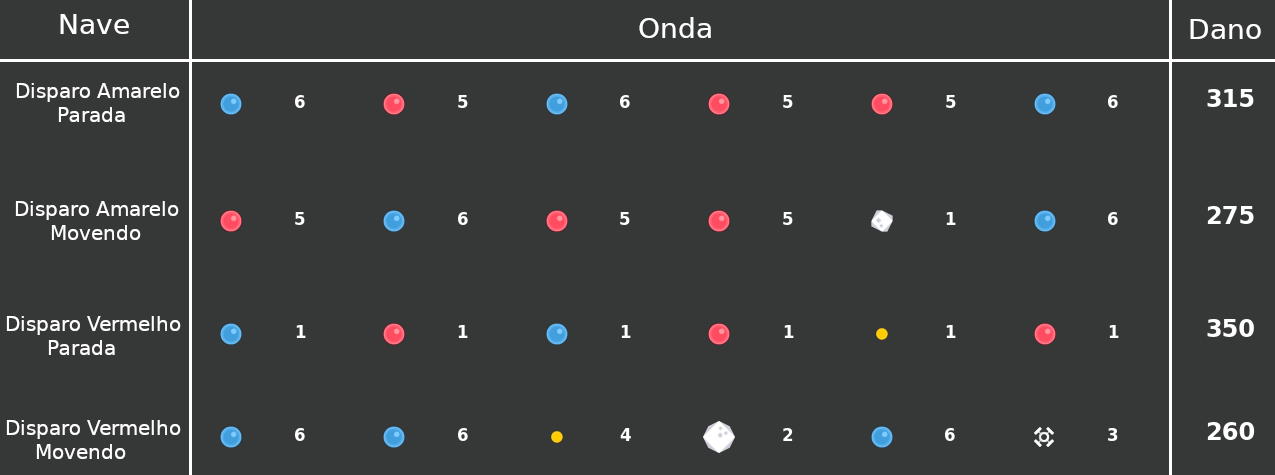
\includegraphics[width=1.0\textwidth]{ss/tab-ss-max.png}
  \caption{Visualização das ondas aleatórias com maior dano no Space Shooter.\label{fig:ss-rd-max}}
\end{figure}

\pagebreak

%% ------------------------------------------------------------------------- %%
\section{Fitness dos Jogos}
\label{sec:a-fitness}

\subsection{Fitness e Mutação}
\label{sec:a-fitness-mutacao-usados}

Foram testados três modelos de \textit{fitness} no algoritmo genético para o jogo \textit{Tower Defense}, buscando obter melhores resultados na geração de ondas; enquanto o jogo \textit{Space Shooter} foi testado somente com a primeira e a terceira versão. Foi adotada uma nomenclatura de versões para simplificar as referências no texto:

\begin{table}
\centering
\begin{tabular}{l|l|l}
                            & \textit{Fitness} (v1) & \textit{Fitness} (v2)  \\ \hline
Taxa de mutação (v1)             & TD e SS          & -                      \\
Taxa de mutação (v2)             &      -           & TD                     \\
Taxa de mutação (v3)             &      SS          & TD          

\end{tabular}
\caption{Relação dos fitness e taxa de mutação usados no TD e SS.}
\label{tab:fit-names}
\end{table}

%% ------------------------------------------------------------------------- %%
\subsection{Tower Defense - Fitness e Mutação}
\label{sec:td-fit}

O primeiro teste realizado utilizou uma função \textit{fitness} que considera se o alvo chegou ao final do trajeto e o quanto do trajeto foi percorrido, indivíduos que completaram o percurso serão muito mais recompensados e aqueles que morreram muito longe do alvo tendem a ser eliminados da população. A taxa de mutação decai conforme o tempo, começando em \textit {mutation\_prob} = 1.0 (100\%) e decrementando até 0. A taxa de mutação volta para 100\% a cada repetição do experimento (30 ondas). 

\begin{programruledcaption}{\textit{Fitness} do primeiro teste do \textit{TD} (v1).\label{prog:avaliacao_TD1}}
  \begin{lstlisting}[
    language={[brazilian]pseudocode},
    style=pseudocode,
    style=wider,
    functions={},
    specialidentifiers={},
  ]
        funcao fitness_v1 (x) // Dá uma pontuação para indivíduo \textbf{x}
            // reached\_goal(x) = booleana se chegou ou não ao final do trajeto
            se reached_goal(x)
                fit := 1
            senao
                fit := 0
            
            // offset(x) = quanto do percurso foi completado.
	        fit := (fit + offset(x)) / 2 // média aritmética dos valores de x
	        devolva fit // Um float com uma pontuação no intervalo [0,1].
        fim
  \end{lstlisting}
\end{programruledcaption}

\begin{programruledcaption}{Taxa de mutação do \textit{TD} para o primeiro teste (v1).\label{prog:mutacao_TD1}}
  \begin{lstlisting}[
    language={[brazilian]pseudocode},
    style=pseudocode,
    style=wider,
    functions={},
    specialidentifiers={},
  ]
        funcao mutation_v1 () 
            se mutation_prob >= 0
		        mutation_prob -= 0.05
		    ...
		    // continuação do processo de mutação.
        fim
  \end{lstlisting}
\end{programruledcaption}

Para o segundo teste, a função \textit{fitness} considera a quantidade do trajeto que foi percorrido (\textit{float} de 0 a 1) e a quantidade de vida ao final do trajeto (\textit{float} de 0 a 1), ou seja, inimigos que completarem o percurso serão mais recompensados conforme a quantidade de vida que chegaram ao final do trajeto. Note que indivíduos que morreram no caminho não serão bem recompensados com essa função. Por um erro, a taxa de mutação ficou em 1 a partir da segunda wave, contudo, alguns resultados interessantes foram obtidos também.

\begin{programruledcaption}{\textit{Fitness} do \textit{TD} (v2) (Avaliação, em português).\label{prog:avaliacao_TD2}}
  \begin{lstlisting}[
    language={[brazilian]pseudocode},
    style=pseudocode,
    style=wider,
    functions={},
    specialidentifiers={},
  ]
        funcao fitness_TD_v2 (x) // Dá uma pontuação para indivíduo \textbf{x}
            // offset(x) = quanto do trajeto foi percorrido, float de 0 a 1.
            // hp (x) = quanto de HP sobrou do inimigo, float de 0 a 1.
	        fit := (offset(x) + hp(x)) / 2 // média aritmética dos valores de x
	        devolva fit // Pontuação no intervalo [0,1].
        fim
  \end{lstlisting}
\end{programruledcaption}


\begin{programruledcaption}{Taxa de mutação do \textit{TD} para cada bateria de testes (2º par dos gráficos).\label{prog:mutacao_TD2}}
  \begin{lstlisting}[
    language={[brazilian]pseudocode},
    style=pseudocode,
    style=wider,
    functions={},
    specialidentifiers={},
  ]
        funcao mutation_v2 () 
            se geração = 1
		        mutation_prob := 1 / 12
		        
		    senão
		        mutation_prob := 1.0
		    ...
		    // continuação do processo de mutação.
        fim
  \end{lstlisting}
\end{programruledcaption}

Para o terceiro teste, a função \textit{fitness} considera a quantidade do trajeto que foi percorrido (float de 0 a 1) e a quantidade de vida ao final do trajeto (float de 0 a 1), idêntico ao anterior. Contudo, a taxa de mutação permanece em um valor fixo equivalente a $\frac{1}{12}$, conforme embasamento no estudo de \citet{haupt00:mutationprob}.

\begin{programruledcaption}{\textit{Fitness} do \textit{TD} (v3) (Avaliação, em português).\label{prog:avaliacao_TD3}}
  \begin{lstlisting}[
    language={[brazilian]pseudocode},
    style=pseudocode,
    style=wider,
    functions={},
    specialidentifiers={},
  ]
        funcao fitness_TD_v3 (x) // Dá uma pontuação para indivíduo \textbf{x}
            // offset (x) = quanto do trajeto foi percorrido, float de 0 a 1.
            // hp (x) = quanto de HP sobrou do inimigo, float de 0 a 1.
	        fit := ( offset (x) + hp (x)) / 2 // média aritmética dos valores de x
	        devolva fit // Pontuação no intervalo [0,1].
        fim
  \end{lstlisting}
\end{programruledcaption}

\begin{programruledcaption}{Taxa de mutação  v3 do \textit{TD} para cada bateria de testes (3º par dos gráficos).\label{prog:mutacao_TD3}}
  \begin{lstlisting}[
    language={[brazilian]pseudocode},
    style=pseudocode,
    style=wider,
    functions={},
    specialidentifiers={},
  ]
        funcao mutation_v3 () 
            mutation_prob := 1 / 12
		    ...
		    // continuação do processo de mutação.
        fim
  \end{lstlisting}
\end{programruledcaption}

%% ------------------------------------------------------------------------- %%
\subsection{Space Shooter - Fitness e Mutação}
\label{sec:ss-fit}

Conforme a Tabela \ref{tab:fit-names}, temos uma única função \textit{fitness} e as mesmas taxas de mutação 1 e 2 apresentadas na subseção anterior.

\begin{programruledcaption}{\textit{Fitness} de todos os testes do \textit{SS} (v1).\label{prog:avaliacao_SS1}}
  \begin{lstlisting}[
    language={[brazilian]pseudocode},
    style=pseudocode,
    style=wider,
    functions={},
    specialidentifiers={},
  ]
        funcao fitness_v1 (x) // Dá uma pontuação para indivíduo \textbf{x}
            // reached\_goal(x) = booleana se acertou o inimigo
            se reached_goal(x)
                fit := 5
            senao
                fit := 0
            
            // hp (x) = 5 * quanto de HP restou ao final da rodada.
	        fit := (fit + hp (x)) / 10 // média aritmética dos valores de x
	        devolva fit // Um float com uma pontuação no intervalo [0,1].
        fim
  \end{lstlisting}
\end{programruledcaption}%CONSERTADO, EU ACHO


%% ------------------------------------------------------------------------- %%
\section{Avaliação dos Testes de Versões de Algoritmo Genético}
\label{sec:fit-res}

 Para a avaliação dos algoritmos genéticos testados, foram gerados gráficos com a média de dano de cada i-ésimas ondas (de 1 até 30) e uma linha contínua com a regressão polinomial de grau 5 (\ref{prog:polyfit}), para os 30 experimentos em cada versão testada.
 
 Analisando os gráficos obteve-se a onda em que ocorreu a convergência do algoritmo, isto é, o ponto a partir do qual o dano causado pela onda ficou estável e aproximadamente linear.\footnote{Através de análise visual das linha de regressão polinomial, procurou-se o primeiro ponto de mínimo ou máximo - dependendo do comportamento crescente ou decrescente do algoritmo - a partir do qual a curva se mantinha razoavelmente estável. Testes que apresentaram resultados constantemente crescentes, decrescentes ou oscilantes foram considerados instáveis, onde o algoritmo nunca convergiu}

\begin{programruledcaption}{Trecho do código para cálculo da regressão polinomial.\label{prog:polyfit}}
  \begin{lstlisting}[
    language={Python},
  ]
    from numpy.polynomial import Polynomial
    
    fit = Polynomial.fit(df_1['wave number'], df_1['average damage'], deg=5)
  \end{lstlisting}
\end{programruledcaption}

A partir dos mesmos dados sem qualquer processamento - isto é, informações de 300 ondas com 6 ou 12 inimigos e o dano causado - foram gerados gráficos de \textit{boxplot}\footnote{Representação gráfica de localidade, viés e dispersão através dos quartis} padrão, com a média representada por quadrados vermelhos. Nestes é possível verificar a dispersão dos danos gerados pelo algoritmo, afim de verificar se o mesmo tende a chegar no mesmo resultado com consistência (indicados no gráfico por "caixas" mais compactas pois mais resultados de ondas se concentrariam de maneira próxima), ou se produz muitos resultados discrepantes, seja com dano muito alto ou muito baixo (graficamente seriam "caixas" longas, ou \textit{outliers}), e onde estão a a maior parte das soluções encontradas (onde a mediana divide os 30 experimentos pela metade e indica onde estão os resultados de dano mais frequente, enquanto a média pode ser influenciada por \textit{outliers}).

%% ------------------------------------------------------------------------- %%
\subsection{Tower Defense - Resultados}
\label{sec:td-fit-res}

Os gráficos seguintes (\ref{fig:fit-td-verde}, \ref{fig:fit-td-verm}, \ref{fig:fit-td-verd-verm} e \ref{fig:fit-td-verm-verd}) apresentam os resultados dos quatro casos de teste no jogo \textit{Tower Defense}, para as três opções citadas em \ref{sec:a-fitness-mutacao-usados}.

\begin{figure}[H]
  \centering
  \includegraphics[width=1.1\textwidth]{td/Torres Verdes Fitness.png}
  \caption{Gráfico com as médias de dano para cada onda no teste com as Torres Verdes para as versões v1, v2 e v3.}
  \label{fig:fit-td-verde}
\end{figure}

\begin{figure}[H]
  \centering
  \includegraphics[width=1.1\textwidth]{td/Torres Vermelhas Fitness.png}
  \caption{Gráfico com as médias de dano para cada onda no teste com as Torres Vermelhas para as versões v1, v2 e v3.}
  \label{fig:fit-td-verm}
\end{figure}

\begin{figure}[H]
  \centering
  \includegraphics[width=1.1\textwidth]{td/Torres Verdes e Vermelhas Fitness.png}
  \caption{Gráfico com as médias de dano para cada onda no teste com as Torres Verdes + Vermelhas para as versões v1, v2 e v3.}
  \label{fig:fit-td-verd-verm}
\end{figure}

\begin{figure}[H]
  \centering
  \includegraphics[width=1.1\textwidth]{td/Torres Vermelhas e Verdes Fitness.png}
  \caption{Gráfico com as médias de dano para cada onda no teste com as Torres Vermelhas + Verdes para as versões v1, v2 e v3.}
  \label{fig:fit-td-verm-verd}
\end{figure}

As Figuras \ref{fig:td-box-green}, \ref{fig:td-box-red}, \ref{td-box-gr} e \ref{td-box-rg} a seguir mostram o comportamento, em cada teste, do dano total de cada i-ésima onda, cada uma sendo representada num \textit{boxplot}.

\vfill
\pagebreak

\begin{figure}[H]
  \centering
  \includegraphics[width=1.1\textwidth]{figuras/td/boxplot Torres Verdes.png}
  \caption{Boxplot do dano das 30 ondas nos 30 experimentos, para as versões v1, v2 e v3.}
  \label{fig:td-box-green}
\end{figure}

\begin{figure}[H]
  \centering
  \includegraphics[width=1.1\textwidth]{figuras/td/boxplot Torres Vermelhas.png}
  \caption{Boxplot do dano das 30 ondas nos 30 experimentos, para as versões v1, v2 e v3.}
  \label{fig:td-box-red}
\end{figure}

\begin{figure}[H]
  \centering
  \includegraphics[width=1.1\textwidth]{figuras/td/boxplot Torres Verde + Vermelha.png}
  \caption{Boxplot do dano das 30 ondas nos 30 experimentos, para as versões v1, v2 e v3.}
  \label{td-box-gr}
\end{figure}

\begin{figure}[H]
  \centering
  \includegraphics[width=1.1\textwidth]{figuras/td/boxplot Torres Vermelha + Verde.png}
  \caption{Boxplot do dano das 30 ondas nos 30 experimentos, para as versões v1, v2 e v3.}
  \label{td-box-rg}
\end{figure}

A Tabela \ref{tab:td-conver} mostra a onda aproximada onde o algoritmo parece ter convergido, e o dano médio após a estabilidade:

\begin{table}
\centering
\begin{tabular}{l|ll|ll|ll}
\multirow{2}{*}{Torres}                                     & \multicolumn{2}{l|}{v1} & \multicolumn{2}{l|}{v2} & \multicolumn{2}{l}{v3} \\
                                                            & Convergiu  & Dano Médio & Convergiu  & Dano Médio & Convergiu & Dano Médio \\ \hline
Verdes                                                      & 8          & 307.04     & 12         & 478.61     & 8         & 482.57     \\ \cline{1-7}
Vermelha                                                    & 15         & 157.78     & Não        & -          & 12        & 167.44     \\ \cline{1-7}
\begin{tabular}[c]{@{}l@{}}Verde +\\ Vermelha\end{tabular}  & 18         & 463.26     & Não        & -          & 11        & 288.18     \\ \cline{1-7}
\begin{tabular}[c]{@{}l@{}}Vermelha\\  + Verde\end{tabular} & 21         & 459.30     & Não        & -          & 12        & 399.16    
\end{tabular}
\caption{Tabela mostrando a onda onde ocorreu a convergência e o dano médio a partir desse ponto até o final.}
\label{tab:td-conver}
\end{table}

%% ------------------------------------------------------------------------- %%
\subsection{Tower Defense - Comparação}
\label{sec:td-fit-comp}

No \textit{Tower Defense} todas as versões do Algoritmos Genéticos se mostraram adequadas, superando a média da geração aleatória, entretanto no teste com Torres Vermelhas nenhuma superou o maior dano obtido em uma onda do teste \textit{Random}. Contra Torres Verdes existe uma solução ótima óbvia, tanques Verdes (\textit{EnemyGreen}), onde o inimigo com maior resistência (e portanto vida) é o mesmo com o maior dano, e as três versões testadas parecem chegar nesse resultado. 

Individualmente, as seguintes características foram apresentadas:

v1:
\begin{itemize}
  \item Convergência em todos os testes;
  \item Contra Torres Verdes apresenta a maior dispersão comparado com v2 e v3, mas o maior dano médio. Único caso onde a média e mediana ficaram próximas;
  \item Menor dispersão nos outros testes, após convergência;
  \item Exceto contra Torres Verdes, mostra dispersão inicial alta, quando converge concentra o dano no último quartil (Q4) e em \textit{outliers} próximos dos menores valores possíveis nas ondas repetidas, fornecidos na Tabela \ref{sec:uni-td}, mas com mediana acima da média;
  \item Não converge para um estado maximal contra Torres Vermelhas, mas consegue superar o maior dano aleatório (pois o melhor estado maximal detectado pela função \textit{fitness} é priorizar sobrevivência dos tanques ao invés do dano causado no Jogador);
  \item Maior dano, dentre as versões, contra Torres heterogêneas (Verde e Vermelha, Vermelha e Verde);
\end{itemize}

\pagebreak

v2:
\begin{itemize}
  \item Somente converge contra Torres Verdes - onde apresenta o segundo melhor resultado - concentrando resultados na mediana e em \textit{outliers} ligeiramente abaixo;
  \item Nos outros casos estabiliza de maneira oscilante, sem melhorar significativamente em relação a onda inicial, com poucos  \textit{outliers} mas muita dispersão (devido à taxa de mutação ser 100\% após a primeira onda);
  \item Consistente, com médias e medianas próximas.
\end{itemize}

v3:
\begin{itemize}
  \item Convergência em todos os testes, e mais rápida do que v1;
  \item Melhor resultado médio contra Torres Verdes - acima do maior dano aleatório - com dados concentrados no segundo e terceiro quartil, mediana acima da média e alguns \textit{outliers} ligeiramente abaixo;
  \item No teste contra Torres Vermelhas apresenta concentração de resultados entre a mediana no último quartil (Q4) e \textit{outliers} próximos das médias das piores ondas aleatórias;
  \item Apresenta a maior dispersão das versões do algoritmo contra Torres Verde + Vermelha, os quartis se estendendo desde o melhor resultado do v1 até os piores apresentados pelas ondas repetidas (Tabela \ref{sec:uni-td});
  \item Contra Torres Vermelha + Verde também supera o maior dano aleatório, com resultados concentrados entre a medianas no último quartil (Q4) e média, que foi afetada por \textit{outliers}.
\end{itemize}

Os resultados indicam que a versão v1 é bastante consistente, com baixa dispersão em 3 testes, mas corre risco de convergir em resultados longe do ótimo, possivelmente por progressivamente reduzir os genes aos piores candidatos e estabilizar no menos pior (taxa de mutação zera após a 20ª onda).

A última versão testada (v3) mostrou comportamento semelhante ao v1 mas com danos menores, exceto contra Torres Verdes. No restante não foi capaz de eliminar casos extremos onde estabilizou próximo do pior caso, apesar da pequena melhoria contra Torres Verde + Vermelha, provavelmente por reduzir os candidatos aptos por más escolhas, semelhante a v1.

\vfill
\pagebreak

%% ------------------------------------------------------------------------- %%
\subsection{Space Shooter - Resultados}
\label{sec:ss-fit-res}

Os gráficos seguintes (\ref{fig:fit-ss-ys}, \ref{fig:fit-ss-ym}, \ref{fig:fit-ss-rs} e \ref{fig:fit-ss-rm}) apresentam os resultados dos quatro casos de teste no jogo \textit{Space Shooter}, para as três opções citadas em \ref{sec:a-fitness-mutacao-usados}.

\begin{figure}[H]
  \centering
  \includegraphics[width=1.1\textwidth]{ss/Nave Parada com Disparo Amarelo Fitness.png}
  \caption{Gráfico com as médias de dano para cada onda no teste com a Nave Parada, Disparo Amarelo para as versões v1 e v3.}
  \label{fig:fit-ss-ys}
\end{figure}

\begin{figure}[H]
  \centering
  \includegraphics[width=1.1\textwidth]{ss/Nave Movendo com Disparo Amarelo Fitness.png}
  \caption{Gráfico com as médias de dano para cada onda no teste com a Nave Movendo, Disparo Amarelo para as versões v1 e v3.}
  \label{fig:fit-ss-ym}
\end{figure}

\begin{figure}[H]
  \centering
  \includegraphics[width=1.1\textwidth]{ss/Nave Parada Disparo Vermelho Fitness.png}
  \caption{Gráfico com as médias de dano para cada onda no teste com a Nave Parada, Disparo Vermelho para as versões v1 e v3.}
  \label{fig:fit-ss-rs}
\end{figure}

\begin{figure}[H]
  \centering
  \includegraphics[width=1.1\textwidth]{ss/Nave Movendo Disparo Vermelho Fitness.png}
  \caption{Gráfico com as médias de dano para cada onda no teste com a Nave Movendo, Disparo Vermelho para as versões v1 e v3.}
  \label{fig:fit-ss-rm}
\end{figure}




Semelhante a Seção \ref{sec:td-fit-res}, as Figuras \ref{fig:ss-box-green}, \ref{fig:ss-box-red}, \ref{ss-box-gr} e \ref{ss-box-rg} a seguir mostram o comportamento, em cada teste, do dano total de cada i-ésima onda, cada uma sendo representada num \textit{boxplot}.

\begin{figure}
  \centering
  \includegraphics[width=1.1\textwidth]{figuras/ss/boxplot Nave Parada com Disparo Amarelo.png}
  \caption{Boxplot do dano das 30 ondas nos 30 experimentos, para as versões v1 e v3.}
  \label{fig:ss-box-green}
\end{figure}

\begin{figure}
  \centering
  \includegraphics[width=1.1\textwidth]{figuras/ss/boxplot Nave Movendo com Disparo Amarelo.png}
  \caption{Boxplot do dano das 30 ondas nos 30 experimentos, para as versões v1 e v3.}
  \label{fig:ss-box-red}
\end{figure}

\begin{figure}
  \centering
  \includegraphics[width=1.1\textwidth]{figuras/ss/boxplot Nave Parada com Disparo Vermelho.png}
  \caption{Boxplot do dano das 30 ondas nos 30 experimentos, para as versões v1 e v3.}
  \label{ss-box-gr}
\end{figure}

\begin{figure}
  \centering
  \includegraphics[width=1.1\textwidth]{figuras/ss/boxplot Nave Movendo com Disparo Vermelho.png}
  \caption{Boxplot do dano das 30 ondas nos 30 experimentos, para as versões v1 e v3.}
  \label{ss-box-rg}
\end{figure}

A Tabela \ref{tab:ss-conv} mostra a onda aproximada onde o algoritmo parece ter convergido, e o dano médio após a estabilidade:

\begin{table}
\centering
\begin{tabular}{l|ll|ll}
\multirow{2}{*}{Nave}                                              & \multicolumn{2}{l|}{v1} & \multicolumn{2}{l}{v3} \\
                                                                   & Convergiu  & Dano Médio & Convergiu & Dano Médio \\ \hline
\begin{tabular}[c]{@{}l@{}}Disparo Amarelo\\ Parada\end{tabular}   & 18         & 163.54     & 13        & 147.66     \\
\begin{tabular}[c]{@{}l@{}}Disparo Amarelo\\ Movendo\end{tabular}  & Não        & -          & Não       & -          \\
\begin{tabular}[c]{@{}l@{}}Disparo Vermelho\\ Parada\end{tabular}  & Não        & -          & Não       & -          \\
\begin{tabular}[c]{@{}l@{}}Disparo Vermelho\\ Movendo\end{tabular} & Não        & -          & Não       & -         
\end{tabular}
\caption{Tabela mostrando a onda onde ocorreu a convergência e o dano médio a partir desse ponto até o final.}
\label{tab:ss-conv}
\end{table}


%% ------------------------------------------------------------------------- %%
\subsection{Space Shooter - Comparação}
\label{sec:ss-fit-comp}

No \textit{Space Shooter} nenhuma versão do algoritmo genético se mostrou adequada pois as ondas convergiram em um ponto não maximal de dano causado, e, em somente um caso, conseguiram dano maior do que na geração aleatória, nunca atingindo o dano máximo de uma dessas ondas. Individualmente, as seguintes características foram apresentadas:

v1
\begin{itemize}
  \item Consegue obter o mesmo dano da onda aleatória em dois testes - Nave Parada com Disparo Amarelo e com Disparo Vermelho;
  \item Com Disparo Amarelo apresenta alta dispersão e poucos \textit{outliers}, com média acima da mediana;
  \item Em particular, com a Nave Parada o algoritmo converge a um resultado não maximal, mas consegue gerar ondas de dano total próximo do máximo teórico (360) \ref{sec:uni-ss} (possivelmente, por priorizar os inimigos que sobrevivem mais ao invés de os que causam mais dano, uma vez que a função \textit{fitness} não prioriza o dano que cada tipo de inimigo causa);
  \item Em geral estabiliza de maneira oscilante, com ondas melhores e piores de maneira sequencial, e médias acima da mediana;
  \item Estabiliza com oscilação e taxa de dano decrescente no teste contra a Nave Parada e Disparo Vermelho, no entanto com diversas ondas que foram totalmente eliminadas, e algumas com dano próximo do máximo (um caso interessante, pois existem alguns tipos de inimigos que sobrevivem melhor em conjunto com outros tipos, mas morrem quando sozinhos e que se reproduz na natureza também, como a co-extinção);
\end{itemize}

\pagebreak

v3
\begin{itemize}
  \item No geral apresenta dispersão menos uniforme do que v1, com maior presença de \textit{outliers};
  \item Com disparo amarelo mantém média bastante acima da mediana, mas não chega a produzir ondas próximas ao máximo como v1, apesar de reduzir ocorrências de inimigos fracos;
  \item Converge no teste com Nave Parada e Disparo Amarelo;
  \item Apresenta o único dano acima da onda aleatória entre todos os testes contra a Nave Parada e Disparo Vermelho, onde possui pouca variação até a onda 10, quando começam \textit{outliers}, e a partir da 20 aumenta drasticamente a dispersão;
  \item Estabiliza de maneira oscilante, com taxa decrescente de dano nos testes com Nave Parada e Disparo Amarelo e Nave Movendo com Disparo Vermelho;
  \item Praticamente empata com o gerador aleatório no teste com a Nave Movendo e Disparo Vermelho, mas de maneira oscilante e viés decrescente, apresentando \textit{outliers} próximos do dano máximo possível.
\end{itemize}

Ambos os \textit{fitness} apresentam comportamento semelhante, onde as ondas iniciais melhoram os resultados coletivos - o dano total - mas progressivamente perdem eficiência, possivelmente devido a tentativa do algoritmo buscar os resultados melhores individuais mas sem a capacidade de detectar que a ordem de aparecimento potencializa o dano, pois a nave só pode atirar no asteroide que apareceu primeiro em seu raio de visão. Logo, é possível que um inimigo lento seguido de outros velozes maximizem o dano de uma rodada, ao "distrair" o jogador, mas que numa avaliação individual essa sequência de inimigos perca para outra onde um inimigo mais forte atingiu o jogador.

O Disparo Vermelho, que possui maior potência, pode ter produzido resultados fracos pois ondas que são totalmente eliminadas não oferecem oportunidade a detecção de candidatos para novas gerações, deixando o algoritmo sem opções de escolha.






\par

%% ------------------------------------------------------------------------- %%
\chapter{Considerações Finais}
\label{cap:consideracoes}

%% ------------------------------------------------------------------------- %%
\section{Análise dos Testes}
\label{sec:analise-testes}

Considerando os danos máximos teóricos e os danos médios dos casos repetidos, apresentados nas seções \ref{sec:uni-td} e \ref{sec:uni-ss}; os danos das ondas aleatórias mostrados em \ref{sec:rd-td} e \ref{sec:rd-ss}; e os testes do algoritmo genético em \ref{sec:td-fit-res} e \ref{sec:ss-fit-res}, utilizando os dados após a convergência dos algoritmos, obtemos as tabelas \ref{tab:td-allres-1} e \ref{tab:td-allres-2}, \ref{tab:ss-allres-1} e \ref{tab:ss-allres-2}:

\pagebreak

\begin{table}[H]
\centering
\begin{tabular}{l|l}
Torres Verdes                & Torres Vermelhas                    \\ \hline
Máximo Calculado = 540.00    & Máximo Calculado = 540.00           \\
\textbf{Fitness v3 = 482.57} & Repetido EnemyGreen = 360.00        \\
\textbf{Fitness v2 = 478.61} & Repetido EnemyBlue = 355.85         \\
Repetido EnemyGreen = 450.00 & Repetido EnemyRed = 180.00          \\
\textbf{Fitness v1 = 307.04} & Repetido OneEach = 167.82           \\
Repetido OneEach = 122.35    & \textbf{Fitness v3 = 167.44}        \\
Repetido EnemyPurple = 90.06 & \textbf{Fitness v1 = 157.78}        \\
Repetido EnemyRed = 89.90    & Repetido EnemyPurple = 127.60       \\
\textbf{Aleatória = 81.42}   & \textbf{Aleatória = 125.35}         \\
Repetido EnemyBlue = 60.68   & Repetido EnemyYellow = 50.58        \\
Repetido EnemyYellow = 40.07 & Repetido EnemyOrange = 50.00        \\
Repetido EnemyOrange = 39.93 & \textbf{Fitness v2 = Não Convergiu}
\end{tabular}
\caption{Dados agregados das médias de todos os testes, ordenado do maior para o menor no Tower Defense}
\label{tab:td-allres-1}
\end{table}

\begin{table}[H]
\centering
\begin{tabular}{l|l}
\begin{tabular}[c]{@{}l@{}}Torres Verde\\  + Vermelha\end{tabular} & \begin{tabular}[c]{@{}l@{}}Torres Vermelha\\   + Verde\end{tabular} \\ \hline
Máximo Calculado = 540.00                                          & Máximo Calculado = 540.00                                           \\
\textbf{Fitness v1 = 463.26}                                       & \textbf{Fitness v1 = 459.30}                                        \\
\textbf{Repetido EnemyGreen = 420.20}                              & Repetido EnemyGreen = 449.85                                        \\
\textbf{Fitness v3 = 288.18}                                       & \textbf{Fitness v3 = 399.16}                                        \\
\textbf{Repetido EnemyBlue = 220.18}                               & Repetido EnemyBlue = 329.82                                         \\
Repetido EnemyRed = 148.50                                         & \textbf{Repetido EnemyRed = 149.90}                                 \\
Repetido OneEach = 148.45                                          & \textbf{Repetido OneEach = 135.05}                                  \\
Repetido EnemyPurple = 120.00                                      & Repetido EnemyPurple = 120.00                                       \\
\textbf{Aleatória = 100.37}                                        & \textbf{Aleatória = 102.37}                                         \\
Repetido EnemyYellow = 50.00                                       & Repetido EnemyYellow = 50.00                                        \\
Repetido EnemyOrange = 44.50                                       & Repetido EnemyOrange = 49.45                                        \\
\textbf{Fitness v2 = Não Convergiu}                                & \textbf{Fitness v2 = Não Convergiu}                                
\end{tabular}
\caption{Dados agregados das médias de todos os testes, ordenado do maior para o menor no Tower Defense}
\label{tab:td-allres-2}
\end{table}

Em apenas 3 casos no jogo \textit{Tower Defense} o algoritmo genético foi capaz de atingir o maior dano, excluindo o dano teórico que só acontece quando o jogador não participa da partida - não faz nenhum tipo de \textit{input} exceto iniciar o jogo. Nos testes com as torres heterogêneas (Verde + Vermelha e Vermelha + Verde) o algoritmo genético com a versão v1 ultrapassou o dano de casos repetidos e para o caso com Torres Verdes a versão v3 consegue causar dano máximo. O projeto não teve como objetivo criar um oponente imbatível, para isso seria mais simples analisar como o jogador dispôs elementos de jogo e a partir disso desenvolver métodos pré-definidos de contra-ataque; ou até mesmo sempre utilizar ondas repetidas que maximizassem o dano, mas tais estratégias poderiam tornar o jogo frustrante ou repetitivo. Fazer com que a composição das ondas de inimigos de adéquem às condições de jogo é mais interessante, e o fato das ondas produzidas sempre superarem as ondas aleatórias neste caso mostram que uma potencial solução está sendo encontrada.

\begin{table}[H]
\centering
\begin{tabular}{l|l}
\begin{tabular}[c]{@{}l@{}}Nave Parada\\ Disparo Amarelo\end{tabular} & \begin{tabular}[c]{@{}l@{}}Nave Movendo\\ Disparo Amarelo\end{tabular} \\ \hline
Máximo Calculado = 360.00                                             & Máximo Calculado = 360.00                                              \\
Inimigo3 = 314.93                                                     & Inimigo3 = 213.20                                                      \\
Inimigo2 = 299.78                                                     & Inimigo2 = 184.61                                                      \\
OneEach = 82.75                                                       & Inimigo1 = 130.10                                                      \\
Inimigo1 = 181.50                                                     & \textbf{Aleatório = 124.95}                                            \\
\textbf{Aleatório = 181.26}                                           & OneEach = 100.85                                                       \\
\textbf{Fitness v1 = 163.54}                                          & Inimigo4 = 80.69                                                       \\
\textbf{Fitness v2 = 147.66}                                          & Inimigos = 67.79                                                       \\
Inimigo4 = 120.00                                                     & Inimigo5 = 39.23                                                       \\
Inimigos = 120.00                                                     & \textbf{Fitness v1 = Não convergiu}                                    \\
Inimigo5 = 60.00                                                      & \textbf{Fitness v2 = Não convergiu}                                   
\end{tabular}
\caption{Dados agregados das médias de todos os testes, ordenado do maior para o menor no Space Shooter}
\label{tab:ss-allres-1}
\end{table}

\begin{table}[H]
\centering
\begin{tabular}{l|l}
\begin{tabular}[c]{@{}l@{}}Nave Parada\\ Disparo Vermelho\end{tabular} & \begin{tabular}[c]{@{}l@{}}Nave Movendo\\ Disparo Vermelho\end{tabular} \\ \hline
Máximo Calculado = 360.00                                              & Máximo Calculado = 360.00                                               \\
\textbf{Inimigo3 = 241.60}                                             & Inimigo3 = 169.87                                                       \\
\textbf{Inimigo2 = 240.94}                                             & Inimigo2 = 169.67                                                       \\
OneEach = 125.99                                                       & OneEach = 96.99                                                         \\
\textbf{Aleatório = 123.66}                                            & \textbf{Aleatório = 91.77}                                              \\
Inimigo4 = 106.00                                                      & \textbf{Inimigo4 = 76.29}                                               \\
Inimigos = 102.44                                                      & \textbf{Inimigos = 65.89}                                               \\
Inimigo5 = 62.57                                                       & Inimigo5 = 39.26                                                        \\
\textbf{Inimigo1 = 27.60}                                              & \textbf{Inimigo1 = 24.60}                                               \\
\textbf{Fitness v1 = Não convergiu}                                    & \textbf{Fitness v1 = Não convergiu}                                     \\
\textbf{Fitness v2 = Não convergiu}                                    & \textbf{Fitness v2 = Não convergiu}                                     \\
Repetido EnemyOrange = 39.93                                           & \textbf{Fitness v2 = Não Convergiu}                                    
\end{tabular}
\caption{Dados agregados das médias de todos os testes, ordenado do maior para o menor no Space Shooter}
\label{tab:ss-allres-2}
\end{table}

Em contraponto, no jogo \textit{Space Shooter}, nenhuma versão consegue convergir em danos acima das ondas aleatórias, apesar de demonstrar potencial para isso contra a Nave Parada com Disparo Vermelho, mostrada no Gráfico \ref{fig:fit-ss-rs} - a taxa de dano é decrescente neste caso, então é possível que com mais ondas o algoritmo piore em relação ao aleatório. Em particular, nos testes com a Nave Parada e Disparo Amarelo (Gráfico \ref{fig:fit-ss-ys}) e Nave Parada com Disparo Vermelho (Gráfico \ref{fig:fit-ss-rs}) a versão v3 conseguiu aumentar o dano nas primeiras ondas, o que pode indicar compatibilidade em partidas curtas ou com redução mais agressiva na possibilidade de mutação, mas seriam necessários testes para confirmar tal possibilidade. No geral, é possível que a natureza menos determinística do estilo de jogo - onde é possível se movimentar para evadir inimigos, deixar de atacar algum oponente pra focar em outro, faça com que o algoritmo genético não seja tão eficiente quanto no \textit{Tower Defense}, que é um jogo mais estático e de comportamento bem definido - as torres não podem ser alteradas durante a onda, e todos os inimigos devem ser atacados para uma defesa efetiva. Seria possível alterar propriedades do \textit{Space Shooter} para diminuir a aleatoriedade da partido - por exemplo, pré-definir pontos de \textit{spawn} dos inimigos - mas acreditou-se que tais mudanças alterariam a natureza do jogo para forçar este se adequar ao projeto. Outro ponto levantado foi em relação à adequação da função \textit{fitness} que poderia levar em conta o dano causado pelos inimigos, já que a função prioriza muito a sobrevivência ao invés desse fator importante de métrica e os inimigos que mais sobrevivem eram justamente os que causavam menos dano.

%% ------------------------------------------------------------------------- %%
\section{Trabalhos Futuros}
\label{sec:futuro}

Considerando a efetividade do algoritmo genético no \textit{Tower Defense}, seria interessante estender os testes para geração de ondas com mudanças entre elas, pois num jogo normal o jogador iria adicionar ou aprimorar torres; o que implica que o algoritmo genético teria que potencialmente reiniciar o processo de convergência para uma geração ótima diferente do anterior. Também pode ser relevante considerar o dano coletivo ao invés de somente o individual dos inimigos, dando possibilidade do algoritmo detectar que está desviando de um estado maximal. Outro ponto que foi excluído por questões de tempo foram testes reais, com jogadores humanos, para obter \textit{feedback} sobre pontos como duração de jogo e escala de dificuldade - informações como essas permitiriam ajustes e testes posteriores em áreas como mutação e outros modelos de \textit{fitness} que seriam mais apropriados caso fossem necessários diferentes velocidade de convergência e escalada de dificuldade.

%% ------------------------------------------------------------------------- %%
\section{Conclusão}
\label{sec:conclusao}

Com os resultados obtidos, fica aparente que o algoritmo evolutivo implementado se mostrou mais adequado ao ambiente determinístico do jogo \textit{Tower Defense}, ao invés da aleatoriedade do \textit{Space Shooter}, causados pelas diferentes possibilidades de tiro (depende da primeira detecção do inimigo) e em dois testes da movimentação da nave. Seria possível tornar o \textit{Space Shooter} mais estático, com locais de \textit{spawn} mais distribuídos e pré-definidos, mas ao mesmo tempo o \textit{Tower Defense} deveria se tornar mais dinâmico, com as torres sendo atualizadas e adicionadas, alterando o ambiente onde o algoritmo genético está buscando evoluir. Dentro destes cenários, o projeto termina sem que seja possível verificar quais alterações seriam mais relevantes, tampouco as diversas adaptações que poderiam ser feita no código, buscando aceleração da convergência e evitando fuga de danos maximais. Ficou claro a infinidade de possibilidades a serem exploradas em um projeto com este tema.

De maneira mais pessoal, a primeira dificuldade da realização do trabalho foi a definição da proposta, posto que como grupo, cada um tinha diferentes ideias, porém eram vagas e carecendo de rigor e objetivo necessário. Para buscar desenvolver novas habilidades, além de exercer outras obtidas durante a graduação, o desenvolvimento de uma inteligência artificial para jogos, assim como o desenvolvimento dos jogos em si, pareceu ser uma proposta interessante. Inicialmente o projeto pareceu simples, mas com o decorrer do tempo o entendimento do problema não se mostrou trivial, e foi necessário algum tempo para compreensão da profundidade da proposta. Tempo excessivo foi gasto na obtenção de fontes e literatura sobre o tema, mas talvez parte dele pudesse ter sido melhor aproveitado na implementação, que se alongou para familiarização de todos os membros com o \textit{Godot} e depois para o desenvolvimento dos jogos. Com os jogos prontos e o algoritmo prototipado, a definição dos testes e coleta de dados se mostrou relativamente demorada, mas foram um dos estágios mais interessantes do trabalho, pois a existência de métricas para qualificar o algoritmo se mostrou muito útil e interessante. Apesar do desejo de aprimorar mais o algoritmo e os jogos, não há tempo hábil para o mesmo, mas a experiência se mostrou edificante e enriquecedora, e demonstrou bem como desenvolver um experimento com algum rigor científico.

\par


\par


%%%%%%%%%%%%%%%%%%%%%%%%%%%% APÊNDICES E ANEXOS %%%%%%%%%%%%%%%%%%%%%%%%%%%%%%%%

% Um apêndice é algum conteúdo adicional de sua autoria que faz parte e
% colabora com a ideia geral do texto mas que, por alguma razão, não precisa
% fazer parte da sequência do discurso; por exemplo, a demonstração de um
% teorema intermediário, as perguntas usadas em uma pesquisa qualitativa etc.
%
% Um anexo é um documento que não faz parte da tese (em geral, nem é de sua
% autoria) mas é relevante para o conteúdo; por exemplo, a especificação do
% padrão técnico ou a legislação que o trabalho discute, um artigo de jornal
% apresentando a percepção do público sobre o tema da tese etc.
%
% Os comandos appendix e annex reiniciam a numeração de capítulos e passam
% a numerá-los com letras. "annex" não faz parte de nenhuma classe padrão,
% ele foi criado para este modelo (em annex.sty e utils.tex). Se o
% trabalho não tiver apêndices ou anexos, remova estas linhas.
%
% Diferentemente de \mainmatter, \backmatter etc., \appendix e \annex não
% forçam o início de uma nova página. Em geral isso não é importante, pois
% o comando seguinte costuma ser "\chapter", mas pode causar problemas com
% a formatação dos cabeçalhos. Assim, vamos forçar uma nova página antes
% de cada um deles.

%%%% Apêndices %%%%

\makeatletter
\if@openright\cleardoublepage\else\clearpage\fi
\makeatother

\pagestyle{appendix}

\appendix

%!TeX root=../tese.tex
%("dica" para o editor de texto: este arquivo é parte de um documento maior)
% para saber mais: https://tex.stackexchange.com/q/78101/183146

% Apague as duas linhas abaixo (elas servem apenas para gerar um
% aviso no arquivo PDF quando não há nenhum dado a imprimir) e
% insira aqui o conteúdo dos apêndices do seu trabalho (ou deixe
% este arquivo vazio)

% Os apêndices podem ser inseridos diretamente aqui ou "puxados" de outros
% arquivos.
% Em alguns (raros) casos, pode ser interessante usar \include ao
% invés de \input: https://tex.stackexchange.com/a/32058/183146

%\input{conteudo/...}
%\par

%\providecommand\aviso[1]{
  \clearpage
  \null
  \vfill
  \begin{hyphenrules}{nohyphenation}
    \centering\bfseries\Large
    #1\par
  \end{hyphenrules}
  \vfill
  \clearpage
}

\providecommand\avisoFolhasDeRosto{
  \aviso{
    {\huge Você precisa editar os arquivos no diretório ``\texttt{conteudo}''!}
    \par\bigskip\bigskip\bigskip\bigskip
    Para gerar a capa e demais páginas preliminares no formato correto,
    modifique os arquivos ``\texttt{conteudo/paginas-preliminares.tex}'' e
    ``\texttt{conteudo/metadados.tex}'', usando como base os arquivos
    correspondentes no diretório ``\texttt{conteudo-exemplo}''.
  }
}

\providecommand\avisoCapitulos{
  \aviso{
    Insira o conteúdo dos capítulos do seu trabalho no arquivo
    ``\texttt{capitulos.tex}'' do diretório ``\texttt{conteudo}''.
  }
}

\providecommand\avisoApendices{
  \aviso{
    Insira o conteúdo dos apêndices do seu trabalho no arquivo
    ``\texttt{apendices.tex}'' do diretório ``\texttt{conteudo}''
    (ou comente a linha correspondente em \texttt{tese.tex}).
  }
}

\providecommand\avisoAnexos{
  \aviso{
    Insira o conteúdo dos anexos do seu trabalho no arquivo
    ``\texttt{anexos.tex}'' do diretório ``\texttt{conteudo}''
    (ou comente a linha correspondente em \texttt{tese.tex}).
  }
}

\providecommand\avisoArtigo{
  \aviso{
    Insira o conteúdo do artigo no arquivo ``\texttt{corpo-artigo.tex}''
    do diretório ``\texttt{conteudo}''. Não se esqueça de consultar
    o exemplo no diretório ``\texttt{conteudo-exemplo}'' para a
    definição do título, autoria etc.
  }
}

\providecommand\avisoApresentacao{
  \begin{frame}{Insira o conteúdo!}
  \aviso{
    Insira o conteúdo da apresentação no arquivo ``\texttt{corpo-apresentacao.tex}''
    do diretório ``\texttt{conteudo}''. Não se esqueça de consultar
    o exemplo no diretório ``\texttt{conteudo-exemplo}'' para a
    definição do título, autoria, estrutura etc.
  }
  \end{frame}
}

\providecommand\avisoPoster{
  \aviso{
    Insira o conteúdo do poster no arquivo ``\texttt{corpo-poster.tex}''
    do diretório ``\texttt{conteudo}''. Não se esqueça de consultar
    o exemplo no diretório ``\texttt{conteudo-exemplo}'' para a
    definição do título, autoria, estrutura etc.
  }
}

%\avisoApendices



%% ------------------------------------------------------------------------- %%
\chapter{Moda das Ondas no Tower Defense para versão v1}
\label{sec:apend-moda-td-v1}

Foram calculadas as modas das ondas do \textit{fitness} desenvolvido, para permitir a visualização dos inimigos mais comuns que o algoritmo convergiu.

%% ------------------------------------------------------------------------- %%
\section{Torres Verdes}
\label{sec:apend-moda-td-g-v1}

\begin{figure}[H]
  \centering
  \includegraphics[width=0.9\textwidth]{figuras/td/td_allgreen_ai_mode_1_1.png}
  \caption{Visualização da moda de cada onda com a versão v1 contra Torres Verdes.}
  \label{fig:td-moda-green-1-1}
\end{figure}

\begin{figure}[H]
  \centering
  \includegraphics[width=0.9\textwidth]{figuras/td/td_allgreen_ai_mode_1_2.png}
  \caption{Visualização da moda de cada onda com a versão v1 contra Torres Verdes.}
  \label{fig:td-moda-green-1-2}
\end{figure}

\begin{figure}[H]
  \centering
  \includegraphics[width=0.9\textwidth]{figuras/td/td_allgreen_ai_mode_1_3.png}
  \caption{Visualização da moda de cada onda com a versão v1 contra Torres Verdes.}
  \label{fig:td-moda-green-1-3}
\end{figure}

%% ------------------------------------------------------------------------- %%
\section{Torres Vermelhas}
\label{sec:apend-moda-td-r-v1}

\begin{figure}[H]
  \centering
  \includegraphics[width=0.9\textwidth]{figuras/td/td_allred_ai_mode_1_1.png}
  \caption{Visualização da moda de cada onda com a versão v1 contra Torres Vermelhas.}
  \label{fig:td-moda-red-1-1}
\end{figure}

\begin{figure}[H]
  \centering
  \includegraphics[width=0.9\textwidth]{figuras/td/td_allred_ai_mode_1_2.png}
  \caption{Visualização da moda de cada onda com a versão v1 contra Torres Vermelhas.}
  \label{fig:td-moda-red-1-2}
\end{figure}

\begin{figure}[H]
  \centering
  \includegraphics[width=0.9\textwidth]{figuras/td/td_allred_ai_mode_1_3.png}
  \caption{Visualização da moda de cada onda com a versão v1 contra Torres Vermelhas.}
  \label{fig:td-moda-red-1-3}
\end{figure}

%% ------------------------------------------------------------------------- %%
\section{Torres Verde + Vermelha}
\label{sec:apend-moda-td-gr-v1}

\begin{figure}[H]
  \centering
  \includegraphics[width=0.9\textwidth]{figuras/td/td_greenred_ai_mode_1_1.png}
  \caption{Visualização da moda de cada onda com a versão v1 contra Torres Verdes + Vermelhas.}
  \label{fig:td-moda-greenred-1-1}
\end{figure}

\begin{figure}[H]
  \centering
  \includegraphics[width=0.9\textwidth]{figuras/td/td_greenred_ai_mode_1_2.png}
  \caption{Visualização da moda de cada onda com a versão v1 contra Torres Verdes + Vermelhas.}
  \label{fig:td-moda-greenred-1-2}
\end{figure}

\begin{figure}[H]
  \centering
  \includegraphics[width=0.9\textwidth]{figuras/td/td_greenred_ai_mode_1_3.png}
  \caption{Visualização da moda de cada onda com a versão v1 contra Torres Verdes + Vermelhas.}
  \label{fig:td-moda-greenred-1-3}
\end{figure}

%% ------------------------------------------------------------------------- %%
\section{Torres Vermelha + Verde}
\label{sec:apend-moda-td-rg-v1}

\begin{figure}[H]
  \centering
  \includegraphics[width=0.9\textwidth]{figuras/td/td_redgreen_ai_mode_1_1.png}
  \caption{Visualização da moda de cada onda com a versão v1 contra Torres Vermelhas + Verdes.}
  \label{fig:td-moda-redgreen-1-1}
\end{figure}

\begin{figure}[H]
  \centering
  \includegraphics[width=0.9\textwidth]{figuras/td/td_redgreen_ai_mode_1_2.png}
  \caption{Visualização da moda de cada onda com a versão v1 contra Torres Vermelhas + Verdes.}
  \label{fig:td-moda-redgreen-1-2}
\end{figure}

\begin{figure}[H]
  \centering
  \includegraphics[width=0.9\textwidth]{figuras/td/td_redgreen_ai_mode_1_3.png}
  \caption{Visualização da moda de cada onda com a versão v1 contra Torres Vermelhas + Verdes.}
  \label{fig:td-moda-redgreen-1-3}
\end{figure}
\par

%% ------------------------------------------------------------------------- %%
\chapter{Moda das Ondas no Tower Defense para o v2}
\label{sec:apend-moda-td-v2}

Foram calculadas as modas das ondas do \textit{fitness} desenvolvido, para permitir a visualização dos inimigos mais comuns que o algoritmo convergiu.

%% ------------------------------------------------------------------------- %%
\section{Torres Verdes}
\label{sec:apend-moda-td-g-v2}

\begin{figure}[H]
  \centering
  \includegraphics[width=0.9\textwidth]{figuras/td/td_allgreen_ai_mode_2_1.png}
  \caption{Visualização da moda de cada onda com a versão v2 contra Torres Verdes.}
  \label{fig:td-moda-green-2-1}
\end{figure}

\begin{figure}[H]
  \centering
  \includegraphics[width=0.9\textwidth]{figuras/td/td_allgreen_ai_mode_2_2.png}
  \caption{Visualização da moda de cada onda com a versão v2 contra Torres Verdes.}
  \label{fig:td-moda-green-2-2}
\end{figure}

\begin{figure}[H]
  \centering
  \includegraphics[width=0.9\textwidth]{figuras/td/td_allgreen_ai_mode_2_3.png}
  \caption{Visualização da moda de cada onda com a versão v2 contra Torres Verdes.}
  \label{fig:td-moda-green-2-3}
\end{figure}

%% ------------------------------------------------------------------------- %%
\section{Torres Vermelhas}
\label{sec:apend-moda-td-r-v2}

\begin{figure}[H]
  \centering
  \includegraphics[width=0.9\textwidth]{figuras/td/td_allred_ai_mode_2_1.png}
  \caption{Visualização da moda de cada onda com a versão v2 contra Torres Vermelhas.}
  \label{fig:td-moda-red-2-1}
\end{figure}

\begin{figure}[H]
  \centering
  \includegraphics[width=0.9\textwidth]{figuras/td/td_allred_ai_mode_2_2.png}
  \caption{Visualização da moda de cada onda com a versão v2 contra Torres Vermelhas.}
  \label{fig:td-moda-red-2-2}
\end{figure}

\begin{figure}[H]
  \centering
  \includegraphics[width=0.9\textwidth]{figuras/td/td_allred_ai_mode_2_3.png}
  \caption{Visualização da moda de cada onda com a versão v2 contra Torres Vermelhas.}
  \label{fig:td-moda-red-2-3}
\end{figure}

%% ------------------------------------------------------------------------- %%
\section{Torres Verde + Vermelha}
\label{sec:apend-moda-td-gr-v2}

\begin{figure}[H]
  \centering
  \includegraphics[width=0.9\textwidth]{figuras/td/td_greenred_ai_mode_2_1.png}
  \caption{Visualização da moda de cada onda com a versão v2 contra Torres Verdes + Vermelhas.}
  \label{fig:td-moda-greenred-2-1}
\end{figure}

\begin{figure}[H]
  \centering
  \includegraphics[width=0.9\textwidth]{figuras/td/td_greenred_ai_mode_2_2.png}
  \caption{Visualização da moda de cada onda com a versão v2 contra Torres Verdes + Vermelhas.}
  \label{fig:td-moda-greenred-2-2}
\end{figure}

\begin{figure}[H]
  \centering
  \includegraphics[width=0.9\textwidth]{figuras/td/td_greenred_ai_mode_2_3.png}
  \caption{Visualização da moda de cada onda com a versão v2 contra Torres Verdes + Vermelhas.}
  \label{fig:td-moda-greenred-2-3}
\end{figure}

%% ------------------------------------------------------------------------- %%
\section{Torres Vermelha + Verde}
\label{sec:apend-moda-td-rg-v2}

\begin{figure}[H]
  \centering
  \includegraphics[width=0.9\textwidth]{figuras/td/td_redgreen_ai_mode_2_1.png}
  \caption{Visualização da moda de cada onda com a versão v2 contra Torres Vermelhas + Verdes.}
  \label{fig:td-moda-redgreen-2-1}
\end{figure}

\begin{figure}[H]
  \centering
  \includegraphics[width=0.9\textwidth]{figuras/td/td_redgreen_ai_mode_2_2.png}
  \caption{Visualização da moda de cada onda com a versão v2 contra Torres Vermelhas + Verdes.}
  \label{fig:td-moda-redgreen-2-2}
\end{figure}

\begin{figure}[H]
  \centering
  \includegraphics[width=0.9\textwidth]{figuras/td/td_redgreen_ai_mode_2_3.png}
  \caption{Visualização da moda de cada onda com a versão v2 contra Torres Vermelhas + Verdes.}
  \label{fig:td-moda-redgreen-2-3}
\end{figure}
\par

%% ------------------------------------------------------------------------- %%
\chapter{Moda das Ondas no Tower Defense para a versão v3}
\label{sec:apend-moda-td-v3}

Foram calculadas as modas das ondas do \textit{fitness} desenvolvido, para permitir a visualização dos inimigos mais comuns que o algoritmo convergiu.

%% ------------------------------------------------------------------------- %%
\section{Torres Verdes}
\label{sec:apend-moda-td-g-v3}

\begin{figure}[H]
  \centering
  \includegraphics[width=0.9\textwidth]{figuras/td/td_allgreen_ai_mode_3_1.png}
  \caption{Visualização da moda de cada onda com a versão v3 contra Torres Verdes.}
  \label{fig:td-moda-green-3-1}
\end{figure}

\begin{figure}[H]
  \centering
  \includegraphics[width=0.9\textwidth]{figuras/td/td_allgreen_ai_mode_3_2.png}
  \caption{Visualização da moda de cada onda com a versão v3 contra Torres Verdes.}
  \label{fig:td-moda-green-3-2}
\end{figure}

\begin{figure}[H]
  \centering
  \includegraphics[width=0.9\textwidth]{figuras/td/td_allgreen_ai_mode_3_3.png}
  \caption{Visualização da moda de cada onda com a versão v3 contra Torres Verdes.}
  \label{fig:td-moda-green-3-3}
\end{figure}

%% ------------------------------------------------------------------------- %%
\section{Torres Vermelhas}
\label{sec:apend-moda-td-r-v3}

\begin{figure}[H]
  \centering
  \includegraphics[width=0.9\textwidth]{figuras/td/td_allred_ai_mode_3_1.png}
  \caption{Visualização da moda de cada onda com a versão v3 contra Torres Vermelhas.}
  \label{fig:td-moda-red-3-1}
\end{figure}

\begin{figure}[H]
  \centering
  \includegraphics[width=0.9\textwidth]{figuras/td/td_allred_ai_mode_3_2.png}
  \caption{Visualização da moda de cada onda com a versão v3 contra Torres Vermelhas.}
  \label{fig:td-moda-red-3-2}
\end{figure}

\begin{figure}[H]
  \centering
  \includegraphics[width=0.9\textwidth]{figuras/td/td_allred_ai_mode_3_3.png}
  \caption{Visualização da moda de cada onda com a versão v3 contra Torres Vermelhas.}
  \label{fig:td-moda-red-3-3}
\end{figure}

%% ------------------------------------------------------------------------- %%
\section{Torres Verde + Vermelha}
\label{sec:apend-moda-td-gr-v3}

\begin{figure}[H]
  \centering
  \includegraphics[width=0.9\textwidth]{figuras/td/td_greenred_ai_mode_3_1.png}
  \caption{Visualização da moda de cada onda com a versão v3 contra Torres Verdes + Vermelhas.}
  \label{fig:td-moda-greenred-3-1}
\end{figure}

\begin{figure}[H]
  \centering
  \includegraphics[width=0.9\textwidth]{figuras/td/td_greenred_ai_mode_3_2.png}
  \caption{Visualização da moda de cada onda com a versão v3 contra Torres Verdes + Vermelhas.}
  \label{fig:td-moda-greenred-3-2}
\end{figure}

\begin{figure}[H]
  \centering
  \includegraphics[width=0.9\textwidth]{figuras/td/td_greenred_ai_mode_3_3.png}
  \caption{Visualização da moda de cada onda com a versão v3 contra Torres Verdes + Vermelhas.}
  \label{fig:td-moda-greenred-3-3}
\end{figure}

%% ------------------------------------------------------------------------- %%
\section{Torres Vermelha + Verde}
\label{sec:apend-moda-td-rg-v3}

\begin{figure}[H]
  \centering
  \includegraphics[width=0.9\textwidth]{figuras/td/td_redgreen_ai_mode_3_1.png}
  \caption{Visualização da moda de cada onda com a versão v3 contra Torres Vermelhas + Verdes.}
  \label{fig:td-moda-redgreen-3-1}
\end{figure}

\begin{figure}[H]
  \centering
  \includegraphics[width=0.9\textwidth]{figuras/td/td_redgreen_ai_mode_3_2.png}
  \caption{Visualização da moda de cada onda com a versão v3 contra Torres Vermelhas + Verdes.}
  \label{fig:td-moda-redgreen-3-2}
\end{figure}

\begin{figure}[H]
  \centering
  \includegraphics[width=0.9\textwidth]{figuras/td/td_redgreen_ai_mode_3_3.png}
  \caption{Visualização da moda de cada onda com a versão v3 contra Torres Vermelhas + Verdes.}
  \label{fig:td-moda-redgreen-3-3}
\end{figure}
\par

%% ------------------------------------------------------------------------- %%
\chapter{Moda das Ondas no Space Shooter para versão v1}
\label{sec:apend-moda-ss-v1}

Foram calculadas as modas das ondas do \textit{fitness} desenvolvido, para permitir a visualização dos inimigos mais comuns que o algoritmo convergiu.

%% ------------------------------------------------------------------------- %%
\section{Nave Parada com Disparo Amarelo}
\label{sec:apend-moda-ss-ys-v1}

\begin{figure}[H]
  \centering
  \includegraphics[width=0.7\textwidth]{figuras/ss/ss_yellowstill_ai_mode_1_1.png}
  \caption{Visualização da moda de cada onda com a versão v1 contra Nave Parada, Disparo Amarelo.}
  \label{fig:ss-moda-ys-1-1}
\end{figure}

\begin{figure}[H]
  \centering
  \includegraphics[width=0.7\textwidth]{figuras/ss/ss_yellowstill_ai_mode_1_2.png}
  \caption{Visualização da moda de cada onda com a versão v1 contra Nave Parada, Disparo Amarelo.}
  \label{fig:ss-moda-ys-1-2}
\end{figure}

\begin{figure}[H]
  \centering
  \includegraphics[width=0.7\textwidth]{figuras/ss/ss_yellowstill_ai_mode_1_3.png}
  \caption{Visualização da moda de cada onda com a versão v1 contra Nave Parada, Disparo Amarelo.}
  \label{fig:ss-moda-ys-1-3}
\end{figure}

%% ------------------------------------------------------------------------- %%
\section{Nave Movendo com Disparo Amarelo}
\label{sec:apend-moda-ss-ym-v1}

\begin{figure}[H]
  \centering
  \includegraphics[width=0.7\textwidth]{figuras/ss/ss_yellowmove_ai_mode_1_1.png}
  \caption{Visualização da moda de cada onda com a versão v1 contra Nave Movendo, Disparo Amarelo.}
  \label{fig:ss-moda-ym-1-1}
\end{figure}

\begin{figure}[H]
  \centering
  \includegraphics[width=0.7\textwidth]{figuras/ss/ss_yellowstill_ai_mode_1_2.png}
  \caption{Visualização da moda de cada onda com a versão v1 contra Nave Movendo, Disparo Amarelo.}
  \label{fig:ss-moda-ym-1-2}
\end{figure}

\begin{figure}[H]
  \centering
  \includegraphics[width=0.7\textwidth]{figuras/ss/ss_yellowstill_ai_mode_1_3.png}
  \caption{Visualização da moda de cada onda com a versão v1 contra Nave Movendo, Disparo Amarelo.}
  \label{fig:ss-moda-ym-1-3}
\end{figure}

%% ------------------------------------------------------------------------- %%
\section{Nave Parada com Disparo Vermelho}
\label{sec:apend-moda-ss-rs-v1}

\begin{figure}[H]
  \centering
  \includegraphics[width=0.7\textwidth]{figuras/ss/ss_redstill_ai_mode_1_1.png}
  \caption{Visualização da moda de cada onda com a versão v1 contra Nave Parada, Disparo Vermelho.}
  \label{fig:ss-moda-rs-1-1}
\end{figure}

\begin{figure}[H]
  \centering
  \includegraphics[width=0.7\textwidth]{figuras/ss/ss_redstill_ai_mode_1_2.png}
  \caption{Visualização da moda de cada onda com a versão v1 contra Nave Parada, Disparo Vermelho.}
  \label{fig:ss-moda-rs-1-2}
\end{figure}

\begin{figure}[H]
  \centering
  \includegraphics[width=0.7\textwidth]{figuras/ss/ss_redstill_ai_mode_1_3.png}
  \caption{Visualização da moda de cada onda com a versão v1 contra Nave Parada, Disparo Vermelho.}
  \label{fig:ss-moda-rs-1-3}
\end{figure}

%% ------------------------------------------------------------------------- %%
\section{Nave Movendo com Disparo Vermelho}
\label{sec:apend-moda-ss-rm-v1}

\begin{figure}[H]
  \centering
  \includegraphics[width=0.7\textwidth]{figuras/ss/ss_redmove_ai_mode_1_1.png}
  \caption{Visualização da moda de cada onda com a versão v1 contra Nave Movendo, Disparo Vermelho.}
  \label{fig:ss-moda-rm-1-1}
\end{figure}

\begin{figure}[H]
  \centering
  \includegraphics[width=0.7\textwidth]{figuras/ss/ss_redmove_ai_mode_1_2.png}
  \caption{Visualização da moda de cada onda com a versão v1 contra Nave Movendo, Disparo Vermelho.}
  \label{fig:ss-moda-rm-1-2}
\end{figure}

\begin{figure}[H]
  \centering
  \includegraphics[width=0.7\textwidth]{figuras/ss/ss_redmove_ai_mode_1_3.png}
  \caption{Visualização da moda de cada onda com a versão v1 contra Nave Movendo, Disparo Vermelho.}
  \label{fig:ss-moda-rm-1-3}
\end{figure}
\par

%% ------------------------------------------------------------------------- %%
\chapter{Moda das Ondas no Space Shooter para versão v3}
\label{sec:apend-moda-ss-v3}

Foram calculadas as modas das ondas do \textit{fitness} desenvolvido, para permitir a visualização dos inimigos mais comuns que o algoritmo convergiu.

%% ------------------------------------------------------------------------- %%
\section{Nave Parada com Disparo Amarelo}
\label{sec:apend-moda-ss-ys-v3}

\begin{figure}[H]
  \centering
  \includegraphics[width=0.7\textwidth]{figuras/ss/ss_yellowstill_ai_mode_2_1.png}
  \caption{Visualização da moda de cada onda com o fitness v3 contra Nave Parada, Disparo Amarelo.}
  \label{fig:ss-moda-ys-2-1}
\end{figure}

\begin{figure}[H]
  \centering
  \includegraphics[width=0.7\textwidth]{figuras/ss/ss_yellowstill_ai_mode_2_2.png}
  \caption{Visualização da moda de cada onda com o fitness v3 contra Nave Parada, Disparo Amarelo.}
  \label{fig:ss-moda-ys-2-2}
\end{figure}

\begin{figure}[H]
  \centering
  \includegraphics[width=0.7\textwidth]{figuras/ss/ss_yellowstill_ai_mode_2_3.png}
  \caption{Visualização da moda de cada onda com o fitness v3 contra Nave Parada, Disparo Amarelo.}
  \label{fig:ss-moda-ys-2-3}
\end{figure}

%% ------------------------------------------------------------------------- %%
\section{Nave Movendo com Disparo Amarelo}
\label{sec:apend-moda-ss-ym-v3}

\begin{figure}[H]
  \centering
  \includegraphics[width=0.7\textwidth]{figuras/ss/ss_yellowmove_ai_mode_2_1.png}
  \caption{Visualização da moda de cada onda com o fitness v3 contra Nave Movendo, Disparo Amarelo.}
  \label{fig:ss-moda-ym-2-1}
\end{figure}

\begin{figure}[H]
  \centering
  \includegraphics[width=0.7\textwidth]{figuras/ss/ss_yellowstill_ai_mode_2_2.png}
  \caption{Visualização da moda de cada onda com o fitness v3 contra Nave Movendo, Disparo Amarelo.}
  \label{fig:ss-moda-ym-2-2}
\end{figure}

\begin{figure}[H]
  \centering
  \includegraphics[width=0.7\textwidth]{figuras/ss/ss_yellowstill_ai_mode_2_3.png}
  \caption{Visualização da moda de cada onda com o fitness v3 contra Nave Movendo, Disparo Amarelo.}
  \label{fig:ss-moda-ym-2-3}
\end{figure}

%% ------------------------------------------------------------------------- %%
\section{Nave Parada com Disparo Vermelho}
\label{sec:apend-moda-ss-rs-v3}

\begin{figure}[H]
  \centering
  \includegraphics[width=0.7\textwidth]{figuras/ss/ss_redstill_ai_mode_2_1.png}
  \caption{Visualização da moda de cada onda com o fitness v3 contra Nave Parada, Disparo Vermelho.}
  \label{fig:ss-moda-rs-2-1}
\end{figure}

\begin{figure}[H]
  \centering
  \includegraphics[width=0.7\textwidth]{figuras/ss/ss_redstill_ai_mode_2_2.png}
  \caption{Visualização da moda de cada onda com o fitness v3 contra Nave Parada, Disparo Vermelho.}
  \label{fig:ss-moda-rs-2-2}
\end{figure}

\begin{figure}[H]
  \centering
  \includegraphics[width=0.7\textwidth]{figuras/ss/ss_redstill_ai_mode_2_3.png}
  \caption{Visualização da moda de cada onda com o fitness v3 contra Nave Parada, Disparo Vermelho.}
  \label{fig:ss-moda-rs-2-3}
\end{figure}

%% ------------------------------------------------------------------------- %%
\section{Nave Movendo com Disparo Vermelho}
\label{sec:apend-moda-ss-rm-v3}

\begin{figure}[H]
  \centering
  \includegraphics[width=0.7\textwidth]{figuras/ss/ss_redmove_ai_mode_2_1.png}
  \caption{Visualização da moda de cada onda com o fitness v3 contra Nave Movendo, Disparo Vermelho.}
  \label{fig:ss-moda-rm-2-1}
\end{figure}

\begin{figure}[H]
  \centering
  \includegraphics[width=0.7\textwidth]{figuras/ss/ss_redmove_ai_mode_2_2.png}
  \caption{Visualização da moda de cada onda com o fitness v3 contra Nave Movendo, Disparo Vermelho.}
  \label{fig:ss-moda-rm-2-2}
\end{figure}

\begin{figure}[H]
  \centering
  \includegraphics[width=0.7\textwidth]{figuras/ss/ss_redmove_ai_mode_2_3.png}
  \caption{Visualização da moda de cada onda com o fitness v3 contra Nave Movendo, Disparo Vermelho.}
  \label{fig:ss-moda-rm-2-3}
\end{figure}
\par
\par

%%%% Anexos %%%%

%\makeatletter
%\if@openright\cleardoublepage\else\clearpage\fi
%\makeatother

%\pagestyle{appendix} % repete o anterior, caso você não use apêndices

%\annex

%%!TeX root=../tese.tex
%("dica" para o editor de texto: este arquivo é parte de um documento maior)
% para saber mais: https://tex.stackexchange.com/q/78101/183146

% Apague as duas linhas abaixo (elas servem apenas para gerar um
% aviso no arquivo PDF quando não há nenhum dado a imprimir) e
% insira aqui o conteúdo dos anexos do seu trabalho (ou deixe este
% arquivo vazio)

% Os anexos podem ser inseridos diretamente aqui ou "puxados" de outros
% arquivos.
% Em alguns (raros) casos, pode ser interessante usar \include ao
% invés de \input: https://tex.stackexchange.com/a/32058/183146

%\input{conteudo/...}
%\par

%\providecommand\aviso[1]{
  \clearpage
  \null
  \vfill
  \begin{hyphenrules}{nohyphenation}
    \centering\bfseries\Large
    #1\par
  \end{hyphenrules}
  \vfill
  \clearpage
}

\providecommand\avisoFolhasDeRosto{
  \aviso{
    {\huge Você precisa editar os arquivos no diretório ``\texttt{conteudo}''!}
    \par\bigskip\bigskip\bigskip\bigskip
    Para gerar a capa e demais páginas preliminares no formato correto,
    modifique os arquivos ``\texttt{conteudo/paginas-preliminares.tex}'' e
    ``\texttt{conteudo/metadados.tex}'', usando como base os arquivos
    correspondentes no diretório ``\texttt{conteudo-exemplo}''.
  }
}

\providecommand\avisoCapitulos{
  \aviso{
    Insira o conteúdo dos capítulos do seu trabalho no arquivo
    ``\texttt{capitulos.tex}'' do diretório ``\texttt{conteudo}''.
  }
}

\providecommand\avisoApendices{
  \aviso{
    Insira o conteúdo dos apêndices do seu trabalho no arquivo
    ``\texttt{apendices.tex}'' do diretório ``\texttt{conteudo}''
    (ou comente a linha correspondente em \texttt{tese.tex}).
  }
}

\providecommand\avisoAnexos{
  \aviso{
    Insira o conteúdo dos anexos do seu trabalho no arquivo
    ``\texttt{anexos.tex}'' do diretório ``\texttt{conteudo}''
    (ou comente a linha correspondente em \texttt{tese.tex}).
  }
}

\providecommand\avisoArtigo{
  \aviso{
    Insira o conteúdo do artigo no arquivo ``\texttt{corpo-artigo.tex}''
    do diretório ``\texttt{conteudo}''. Não se esqueça de consultar
    o exemplo no diretório ``\texttt{conteudo-exemplo}'' para a
    definição do título, autoria etc.
  }
}

\providecommand\avisoApresentacao{
  \begin{frame}{Insira o conteúdo!}
  \aviso{
    Insira o conteúdo da apresentação no arquivo ``\texttt{corpo-apresentacao.tex}''
    do diretório ``\texttt{conteudo}''. Não se esqueça de consultar
    o exemplo no diretório ``\texttt{conteudo-exemplo}'' para a
    definição do título, autoria, estrutura etc.
  }
  \end{frame}
}

\providecommand\avisoPoster{
  \aviso{
    Insira o conteúdo do poster no arquivo ``\texttt{corpo-poster.tex}''
    do diretório ``\texttt{conteudo}''. Não se esqueça de consultar
    o exemplo no diretório ``\texttt{conteudo-exemplo}'' para a
    definição do título, autoria, estrutura etc.
  }
}

%\avisoAnexos

%%!TeX root=../tese.tex
%("dica" para o editor de texto: este arquivo é parte de um documento maior)
% para saber mais: https://tex.stackexchange.com/q/78101/183146

\chapter[Perguntas Frequentes sobre o Modelo]{Perguntas Frequentes sobre o Modelo\footnote{Esta
seção não é de fato um anexo, mas sim um apêndice; ela foi definida desta
forma apenas para servir como exemplo de anexo.}}

\begin{itemize}

\item \textbf{Não consigo decorar tantos comandos!}\\
Use a colinha que é distribuída juntamente com este modelo (\url{gitlab.com/ccsl-usp/modelo-latex/raw/master/pre-compilados/colinha.pdf?inline=false}).

\item \textbf{Por que tantos arquivos?}\\
O preâmbulo \LaTeX{} deste modelo é muito longo; as partes que normalmente não precisam ser modificadas foram colocadas no diretório \texttt{extras}, juntamente com alguns arquivos acessórios. Já os arquivos de conteúdo (capítulos, anexos etc.) foram divididos de maneira que seja fácil para você atualizar o modelo (copiando os novos arquivos ou com um sistema de controle de versões) sem que alterações no conteúdo de exemplo (este texto que você está lendo) causem conflitos com o seu próprio texto.\looseness=-1

\item \textbf{As figuras e tabelas são colocadas em lugares ruins.}\\
Veja a discussão a respeito na Seção~\ref{sec:limitations}.

\item \textbf{Estou tendo problemas com caracteres acentuados.}\\
Versões modernas de \LaTeX{} usam UTF-8, mas arquivos antigos podem usar outras codificações (como ISO-8859-1, também conhecido como latin1 ou Windows-1252). Nesses casos, use \textsf{\textbackslash{}usepackage[latin1]\{inputenc\}} no preâmbulo do documento. Você também pode representar os caracteres acentuados usando comandos \LaTeX{}: \textsf{\textbackslash\textquotesingle{}a} para á, \textsf{\textbackslash{}c\{c\}} para cedilha etc., independentemente da codificação usada no texto\footnote{Você pode consultar os comandos desse tipo mais comuns em \url{en.wikibooks.org/wiki/LaTeX/Special_Characters}. Observe que a dica sobre o pingo do i \emph{não} é mais válida atualmente; basta usar \textsf{\textbackslash\textquotesingle{}i}.}.

\item \textbf{Existe algo específico para citações de páginas web?}\\
Biblatex define o tipo ``online'', que deve ser usado para materiais com título, autor etc., como uma postagem ou comentário em um blog, um gráfico ou mesmo uma mensagem de email para uma lista de discussão. Bibtex\index{bibtex}, por padrão, não tem um tipo específico para isso; com ele, normalmente usa-se o campo ``howpublished'' para especificar que se trata de um recurso \textit{online}. Se o que você está citando não é algo determinado com título, autor etc. mas sim um sítio (como uma empresa ou um produto), pode ser mais adequado colocar a referência apenas como nota de rodapé e não na lista de referências; nesses casos, algumas pessoas acrescentam uma segunda lista de referências especificamente para recursos \textit{online} (biblatex\index{biblatex} permite criar múltiplas bibliografias). Já artigos disponíveis \textit{online} mas que fazem parte de uma publicação de formato tradicional (mesmo que apenas \textit{online}), como os anais de um congresso, devem ser citados por seu tipo verdadeiro e apenas incluir o campo ``url'' (não é nem necessário usar o comando \textsf{\textbackslash{}url\{\}}), aceito por todos os tipos de documento do bibtex/biblatex.

\item \textbf{Aparece uma folha em branco entre os capítulos.}\\
Essa característica foi colocada propositalmente, dado que todo capítulo deve (ou deveria) começar em uma página de numeração ímpar (lado direito do documento). Se quiser mudar esse comportamento, acrescente ``openany'' como opção da classe, i.e., \textsf{\textbackslash{}documentclass[openany,\dots]\{book\}}.

\item \textbf{É possível resumir o nome das seções/capítulos que aparece no topo das páginas e no sumário?}\\
Sim, usando a sintaxe \textsf{\textbackslash{}section[mini-titulo]\{titulo enorme\}}. Isso é especialmente útil nas legendas (\textit{captions}\index{Legendas}) das figuras e tabelas, que muitas vezes são demasiadamente longas para a lista de figuras/tabelas.

\item \textbf{Existe algum programa para gerenciar referências em formato bibtex?}\\
Sim, há vários. Uma opção bem comum é o JabRef; outra é usar Zotero\index{Zotero} ou Mendeley\index{Mendeley} e exportar os dados deles no formato .bib.

\item \textbf{Posso usar pacotes \LaTeX{} adicionais aos sugeridos?}\\
Com certeza! Você pode modificar os arquivos o quanto desejar, o modelo serve só como uma ajuda inicial para o seu trabalho.

\item \textbf{Como faço para usar o Makefile (comando make) no Windows?}\\
Lembre-se que a ferramenta recomendada para compilação do documento é o \textsf{latexmk}, então você não precisa do \textsf{make}. Mas, se quiser usá-lo, você pode instalar o MSYS2 (\url{www.msys2.org}) ou o Windows Subsystem for Linux (procure as versões de Linux disponíveis na Microsoft Store). Se você pretende usar algum dos editores sugeridos, é possível deixar a compilação a cargo deles, também dispensando o \textsf{make}.\looseness=-1

\item \textbf{Como eu faço para...}\\
Leia os comentários dos arquivos ``tese.tex'' e outros que compõem este modelo, além do tutorial %(Capítulo \ref{chap:tutorial})
e dos exemplos do Capítulo %\ref{chap:exemplos}%
; é provável que haja uma dica neles ou, pelo menos, a indicação da \textit{package} relacionada ao que você precisa.

\end{itemize}

%\par



%\par


%%%%%%%%%%%%%%% SEÇÕES FINAIS (BIBLIOGRAFIA E ÍNDICE REMISSIVO) %%%%%%%%%%%%%%%%

% O comando backmatter desabilita a numeração de capítulos.
\backmatter

\pagestyle{backmatter}

% Espaço adicional no sumário antes das referências / índice remissivo
\addtocontents{toc}{\vspace{2\baselineskip plus .5\baselineskip minus .5\baselineskip}}

% A bibliografia é obrigatória

\printbibliography[
  title=\refname\label{bibliografia}, % "Referências", recomendado pela ABNT
  %title=\bibname\label{bibliografia}, % "Bibliografia"
  heading=bibintoc, % Inclui a bibliografia no sumário
]

%\printindex % imprime o índice remissivo no documento (opcional)

\end{document}
